\documentclass{article}

% if you need to pass options to natbib, use, e.g.:
%     \PassOptionsToPackage{numbers, compress}{natbib}
% before loading neurips_2024


% ready for submission
% \usepackage{neurips_2024}
\usepackage[preprint]{neurips_2024}


% to compile a preprint version, e.g., for submission to arXiv, add add the
% [preprint] option:
%     \usepackage[preprint]{neurips_2024}


% to compile a camera-ready version, add the [final] option, e.g.:
%     \usepackage[final]{neurips_2024}


% to avoid loading the natbib package, add option nonatbib:
%    \usepackage[nonatbib]{neurips_2024}


\usepackage[utf8]{inputenc} % allow utf-8 input
\usepackage[T1]{fontenc}    % use 8-bit T1 fonts
\usepackage{hyperref}       % hyperlinks
\usepackage{url}            % simple URL typesetting
\usepackage{booktabs}       % professional-quality tables
\usepackage{amsfonts}       % blackboard math symbols
\usepackage{nicefrac}       % compact symbols for 1/2, etc.
\usepackage{microtype}      % microtypography
\usepackage{xcolor}         % colors
\usepackage{xspace}
\usepackage{amsmath}
\usepackage{amssymb}
\usepackage{mathtools}
\usepackage{amsthm}
\usepackage{float}          % 提供 [H] 选项强制浮动体位置(可用于特殊布局控制)
\usepackage{adjustbox}      % 如果你需要更灵活地控制表格或图像尺寸
\usepackage{graphicx}       % 用于插入图像
\usepackage{caption}        % 提供 \captionof 用于非浮动体的标题
\usepackage{array}          % 表格列格式优化(如 @{} 去掉列间空白)
\usepackage{graphicx}
\usepackage{subfigure}
\usepackage{array}
\usepackage{wrapfig}  % 放在导言区

\usepackage{multirow} 
\usepackage{graphicx}     % figures (if you later embed any)
\usepackage{xspace}       % tidy handling of trailing spaces
\usepackage{url}          % typeset URLs
\usepackage{hyperref}     % clickable links (loads color/driver‑safe options)
\usepackage[table]{xcolor}
\usepackage{enumitem}
\usepackage{listings}     % \begin{lstlisting} … \end{lstlisting}
\newcommand{\method}{\textsc{XX}\xspace}
\newcommand{\draftonly}[1]{#1} 
% Uncomment for submission
% \renewcommand{\draftonly}[1]{}
\newcommand{\draftcomment}[3]{\draftonly{{\textcolor{#3}{[\textbf{#1--\textsc{#2}}]}}}}
\newcommand{\haozhe}[1]{\draftcomment{#1}{Haozhe}{teal}}
\newcommand{\zefan}[1]{\draftcomment{#1}{Zefan}{orange}}
\newcommand{\junjie}[1]{\draftcomment{#1}{Junjie}{purple}}
\usepackage{cleveref}
\crefname{section}{\S}{\S\S}     % lowercase: \cref{...}
\Crefname{section}{\S}{\S\S}     % capitalized: \Cref{...}
\usepackage{subcaption}
\usepackage{marvosym} 
\usepackage{pifont}     % \ding{51} 用于对号
\usepackage{makecell}   % 让表头可换行
\newcommand{\cmark}{\ding{51}} % 对号
\newcommand{\model}{\textsc{Mentor}\xspace}
\newcommand{\ssz}[1]{{\color{red}#1}}

% \title{
%   \begin{minipage}{0.03\textwidth}
%     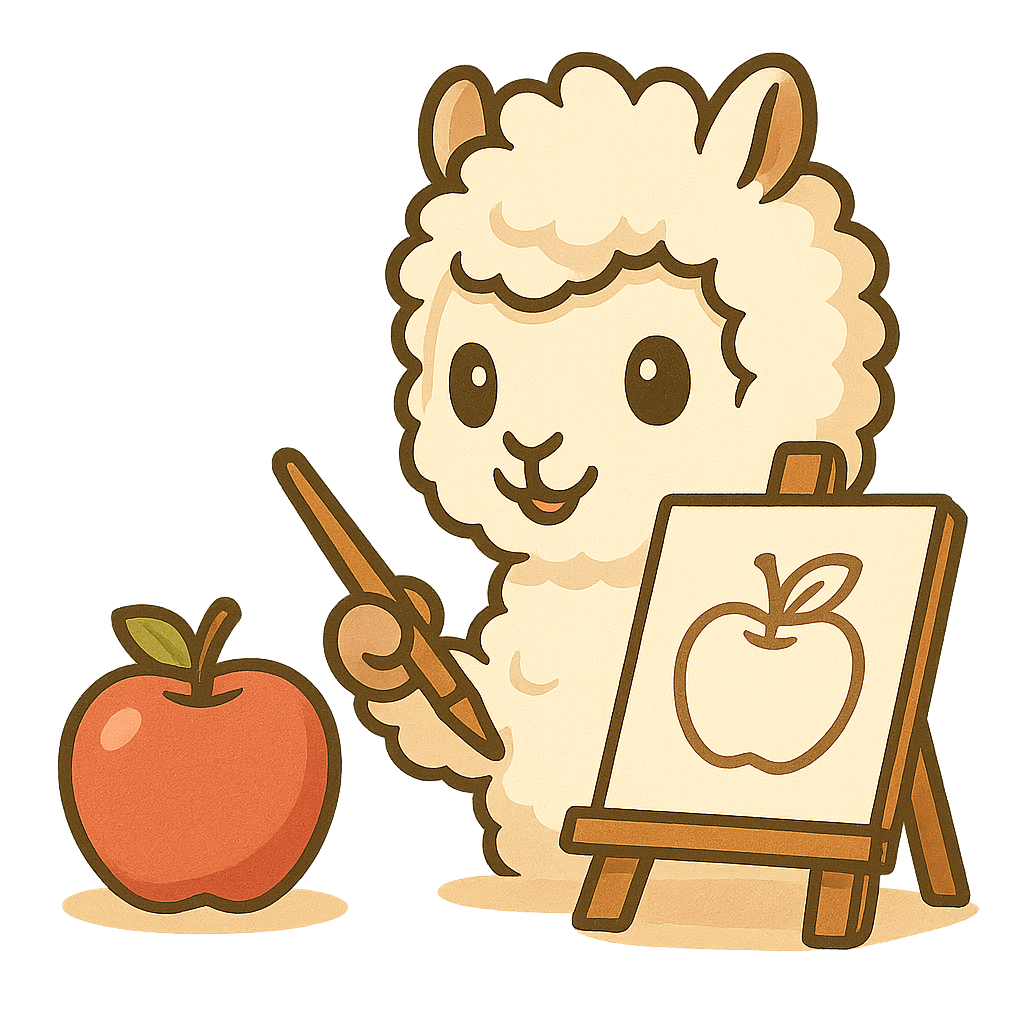
\includegraphics[width=\linewidth]{figures/logo.png}
%   \end{minipage}
%   \hfill
%   \begin{minipage}{0.95\textwidth}
%     \centering
%     \textbf{MENTOR: Efficient Multimodal-Conditioned Tuning for Autoregressive Vision Generation Models}
%   \end{minipage}
% }
\title{MENTOR: Efficient Multimodal-Conditioned Tuning for Autoregressive Vision Generation Models}

% \title{
%     \begin{minipage}{0.2\textwidth}
%         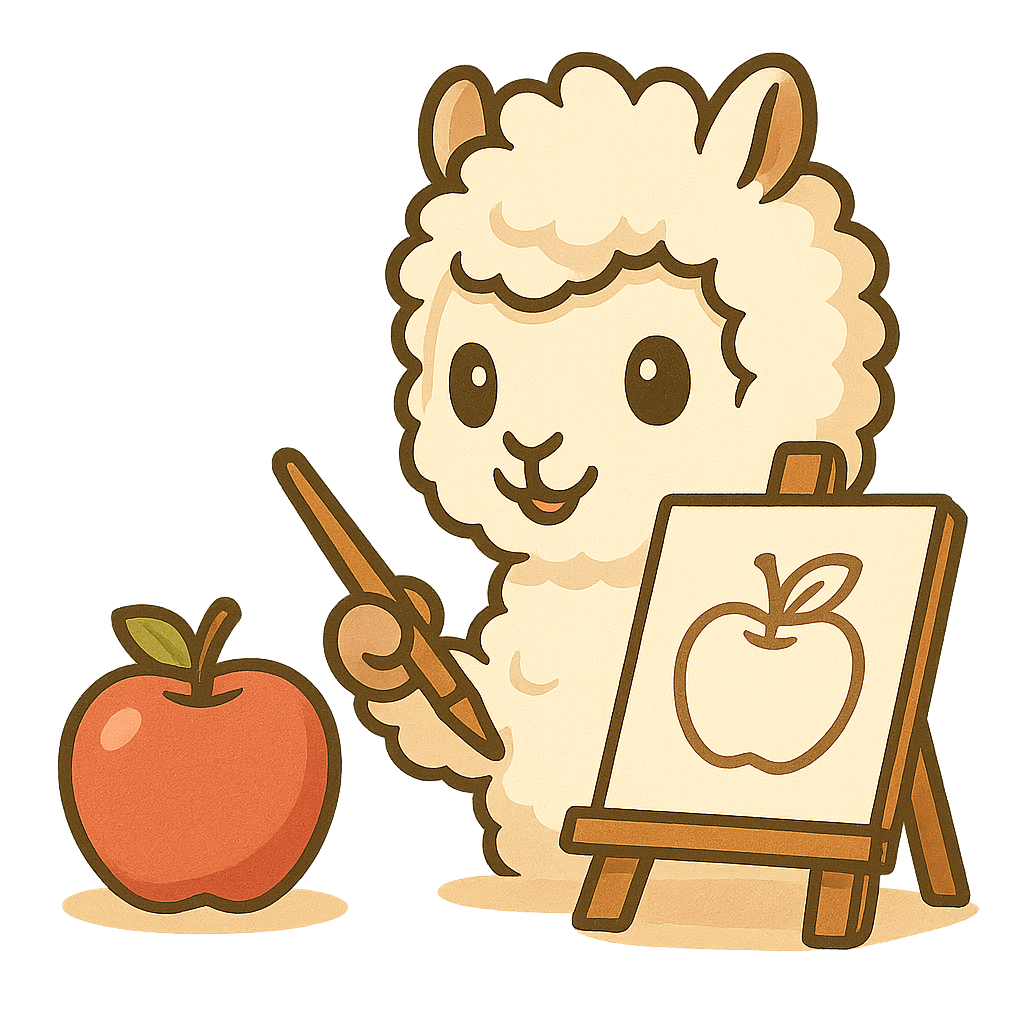
\includegraphics[height=38pt]{figures/logo.png}
%     \end{minipage}
%     \hspace{-0.5in}
%     \begin{minipage}{0.80\textwidth}
%         MENTOR: Efficient Multimodal-Conditioned Tuning for Autoregressive Vision Generation Models
%     \end{minipage}
% }


% The \author macro works with any number of authors. There are two commands
% used to separate the names and addresses of multiple authors: \And and \AND.
%
% Using \And between authors leaves it to LaTeX to determine where to break the
% lines. Using \AND forces a line break at that point. So, if LaTeX puts 3 of 4
% authors names on the first line, and the last on the second line, try using
% \AND instead of \And before the third author name.


% \author{%
%   David S.~Hippocampus\thanks{Use footnote for providing further information
%     about author (webpage, alternative address)---\emph{not} for acknowledging
%     funding agencies.} \\
%   Department of Computer Science\\
%   Cranberry-Lemon University\\
%   Pittsburgh, PA 15213 \\
%   \texttt{hippo@cs.cranberry-lemon.edu} \\
%   % examples of more authors
%   % \And
%   % Coauthor \\
%   % Affiliation \\
%   % Address \\
%   % \texttt{email} \\
%   % \AND
%   % Coauthor \\
%   % Affiliation \\
%   % Address \\
%   % \texttt{email} \\
%   % \And
%   % Coauthor \\
%   % Affiliation \\
%   % Address \\
%   % \texttt{email} \\
%   % \And
%   % Coauthor \\
%   % Affiliation \\
%   % Address \\
%   % \texttt{email} \\
% }
\author{%
    Haozhe Zhao$^{1}$$^\ast$,~~Zefan Cai$^{2}$$^\ast$,~~Shuzheng Si$^{3}$,~~Liang Chen$^{4}$,\\
    ~~\textbf{Jiuxiang Gu}$^{5}$,~~\textbf{Wen Xiao}$^{6}$,~~\textbf{Junjie Hu}$^{2}$
    % $\text{\Letter}$
    \\
    $^{1}$University of Illinois Urbana-Champaign 
$^{2}$University of
Wisconsin-Madison \\
% $^{3}$Department of Computer Science and Technology, Tsinghua University \\
% $^{4}$School of Computer Science, Peking University \\
$^{3}$Tsinghua University
$^{4}$Peking University 
$^{5}$Adobe Research ~~$^{6}$Microsoft \\
    % ~~~\Letter~Corresponding author \\
    \texttt{haozhez6@illinois.edu}\\
    \href{https://mentor.github.io}{\texttt{mentor.github.io}}
}

% \author{%
%     Haozhe Zhao$^{1}$,~~Zefan Cai$^{2}$,~~Shuzheng Si$^{3}$,~~Liang Chen$^{4}$,\\
%     ~~\textbf{Jiuxiang Gu}$^{5}$,~~\textbf{Wen Xiao}$^{6}$,~~\textbf{Junjie Hu}$^{2}$\thanks{Corresponding author: \texttt{junjie.hu@wisc.edu}} \\
%     $^{1}$University of Illinois Urbana-Champaign, 
%     $^{2}$University of Wisconsin-Madison, \\
%     $^{3}$Tsinghua University, 
%     $^{4}$Peking University, 
%     $^{5}$Adobe Research, 
%     $^{6}$Microsoft
% }


\begin{document}


\maketitle
\renewcommand{\thefootnote}{\fnsymbol{footnote}}
\footnotetext[1]{Equal contribution.}

\vspace{-5ex}
\begin{abstract}

Recent text-to-image models produce high-quality results but still struggle with precise visual control, balancing multimodal inputs, and demanding extensive training for complex multimodal image generation.
To address these limitations, we propose \textbf{\model}, a novel autoregressive (AR) framework for efficient \textbf{M}ultimodal-condition\textbf{E}d tu\textbf{N}ing for au\textbf{T}\textbf{O}reg\textbf{R}essive multimodal image generation.
% Our paradigm employs a unified AR transformer that processes interleaved visual and textual inputs to generate images autoregressively and deterministically.
% A lightweight multimodal encoder projects inputs into a shared latent sequence, which a single-stream AR decoder then uses to generate image tokens. 
\model combines an AR image generator with a two-stage training paradigm, enabling fine-grained, token-level alignment between multimodal inputs and image outputs—without relying on auxiliary adapters or cross-attention modules.
Central to our method is the two-stage training paradigm: (1) a \textit{multimodal alignment stage} that establishes robust pixel and semantic-level alignment between inputs and generated tokens, followed by (2) a \textit{multimodal instruction tuning stage} that balance model's integration of multimodal inputs and enhance generation controllability.
Extensive experiments demonstrate that, despite a modest model size, suboptimal base components, and limited training resources, \model achieves a strong balance between concept preservation and prompt following on DreamBench++ benchmark, outperforming competitive baselines. 
Additionally, our method also delivers superior image reconstruction fidelity, broad adaptability across multimodal tasks, and an efficient training budget compared to diffusion-based counterparts. 
The dataset, code, and models are available in \href{https://github.com/HaozheZhao/MENTOR}{\texttt{github.com/HaozheZhao/MENTOR}}.
% This work presents an efficient, controllable, and scalable AR pathway for complex multimodal image generation, offering a compelling alternative to prevalent resource-intensive systems.
% 

\begin{figure*}[htbp]
% \vspace{-1ex}
\centering
% 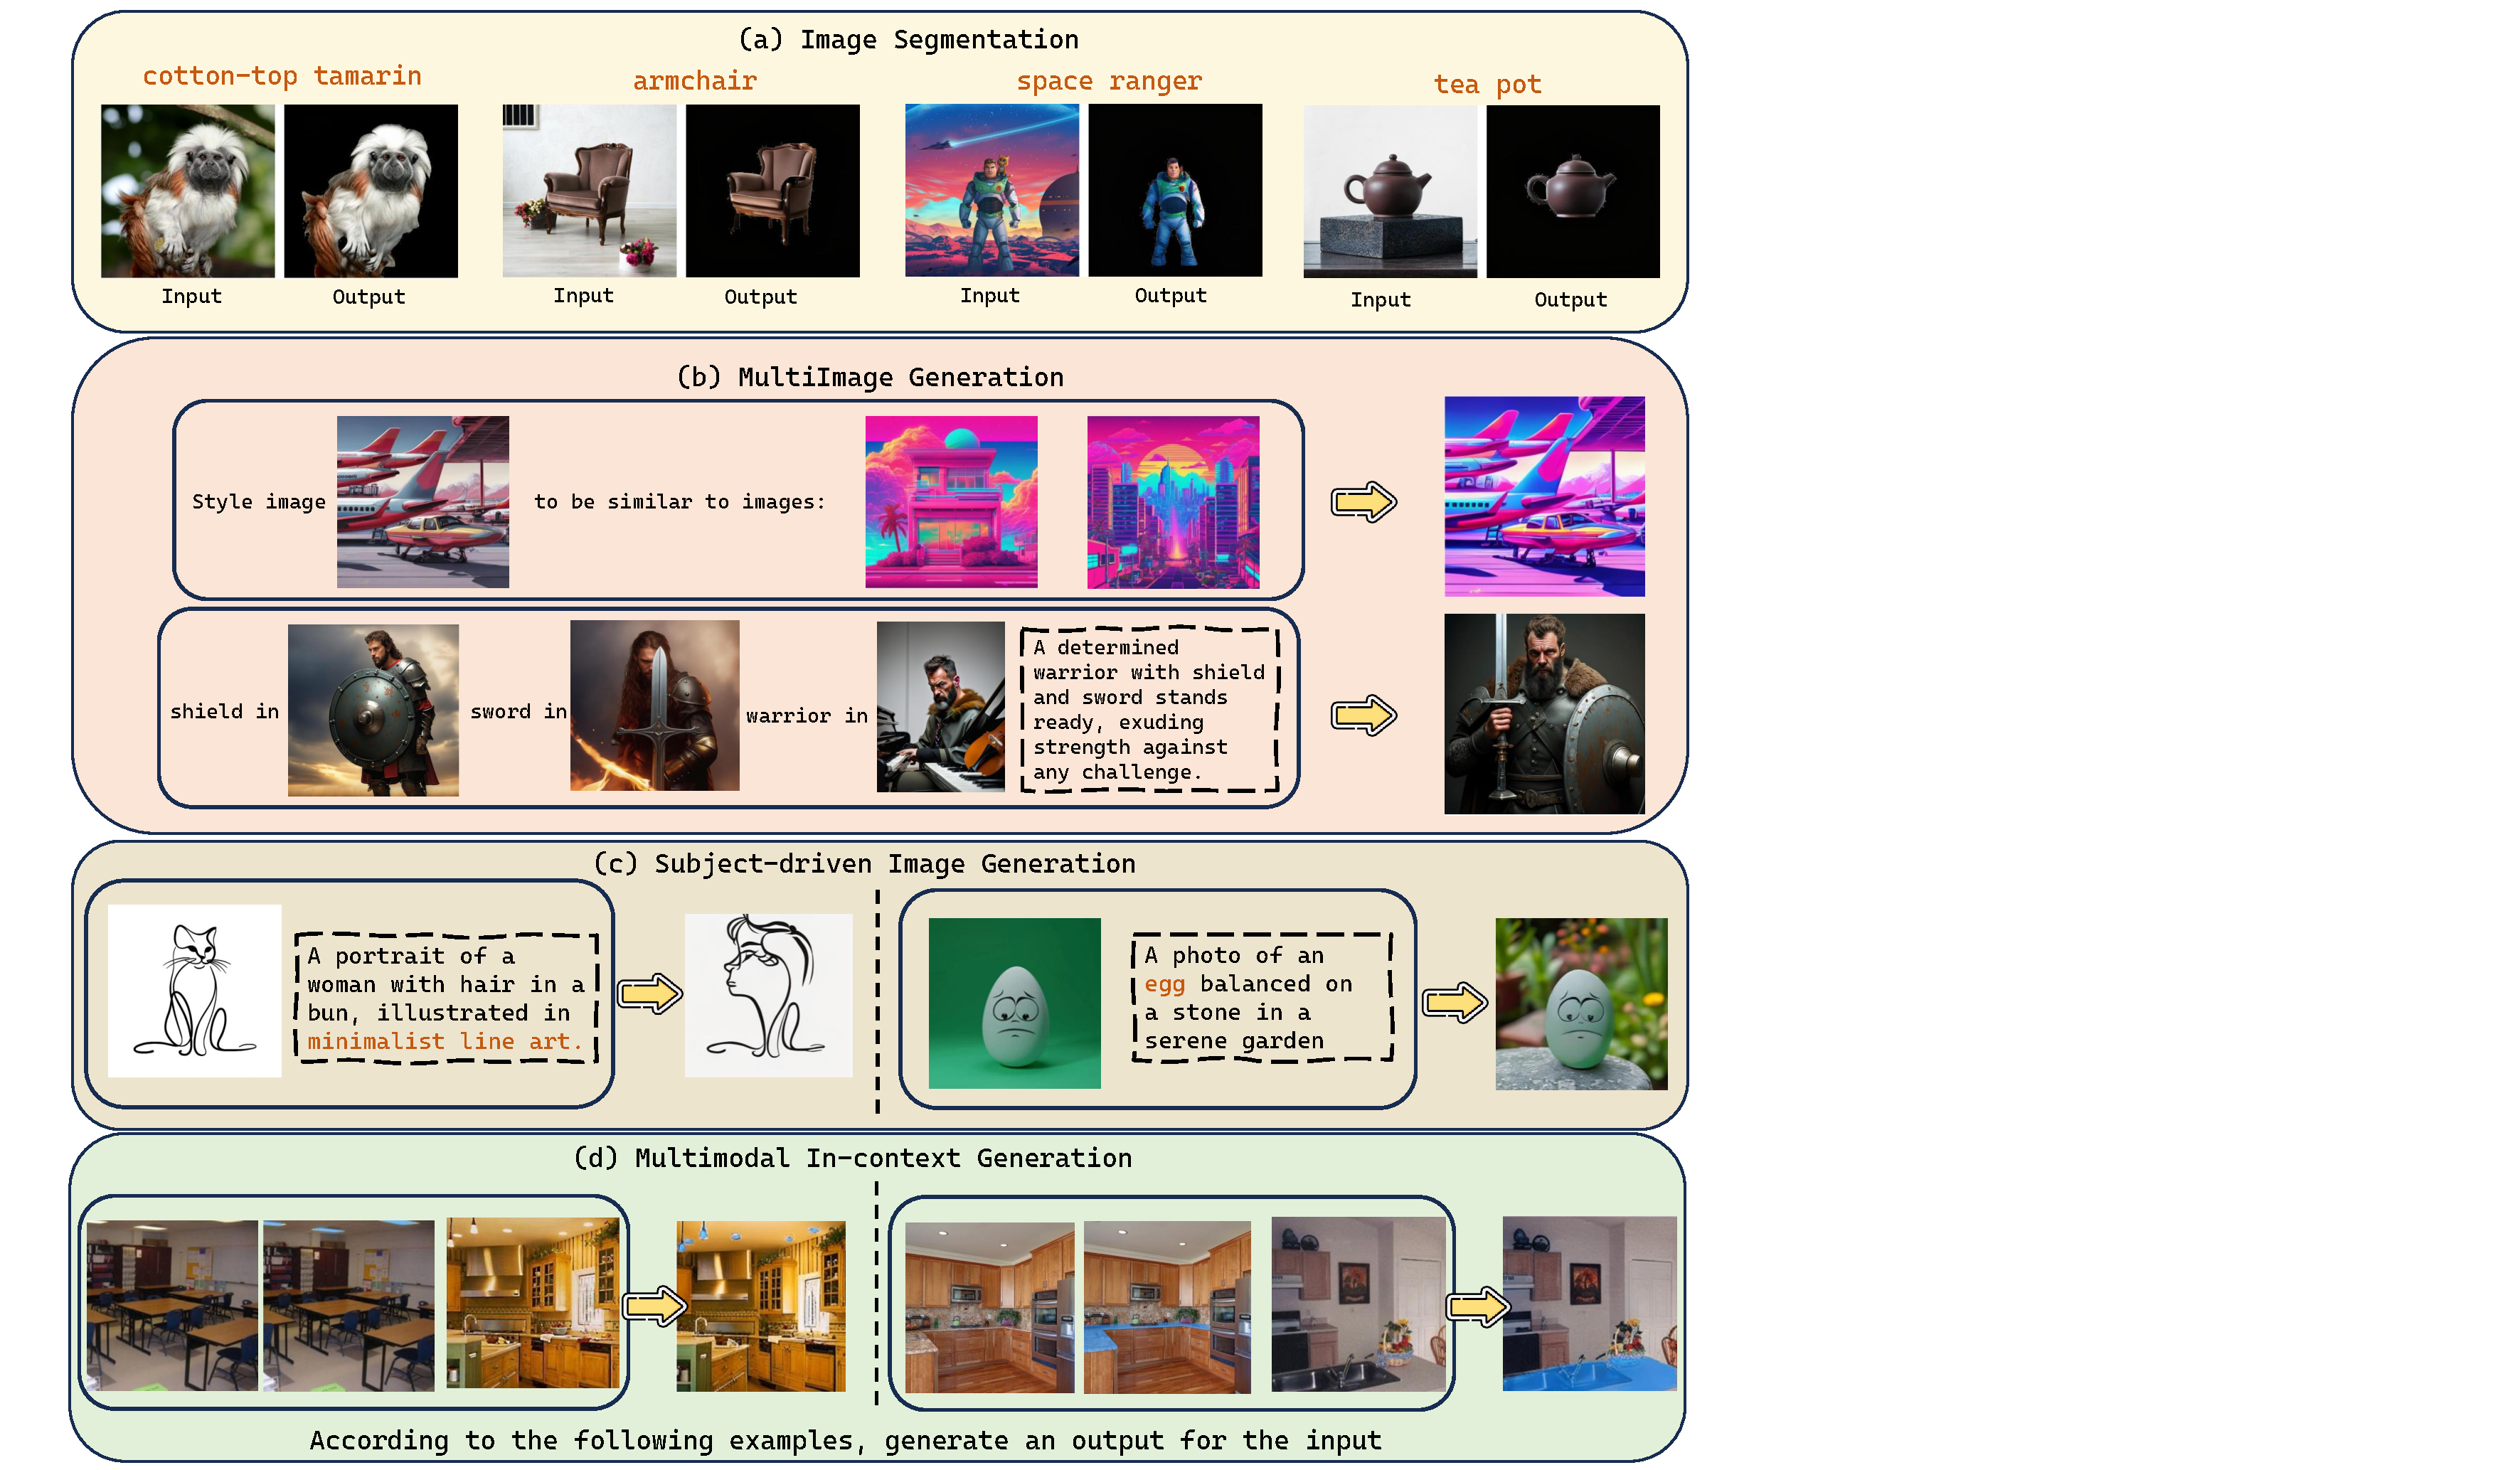
\includegraphics[width=1.0\textwidth]{figures/examples.pdf}
% 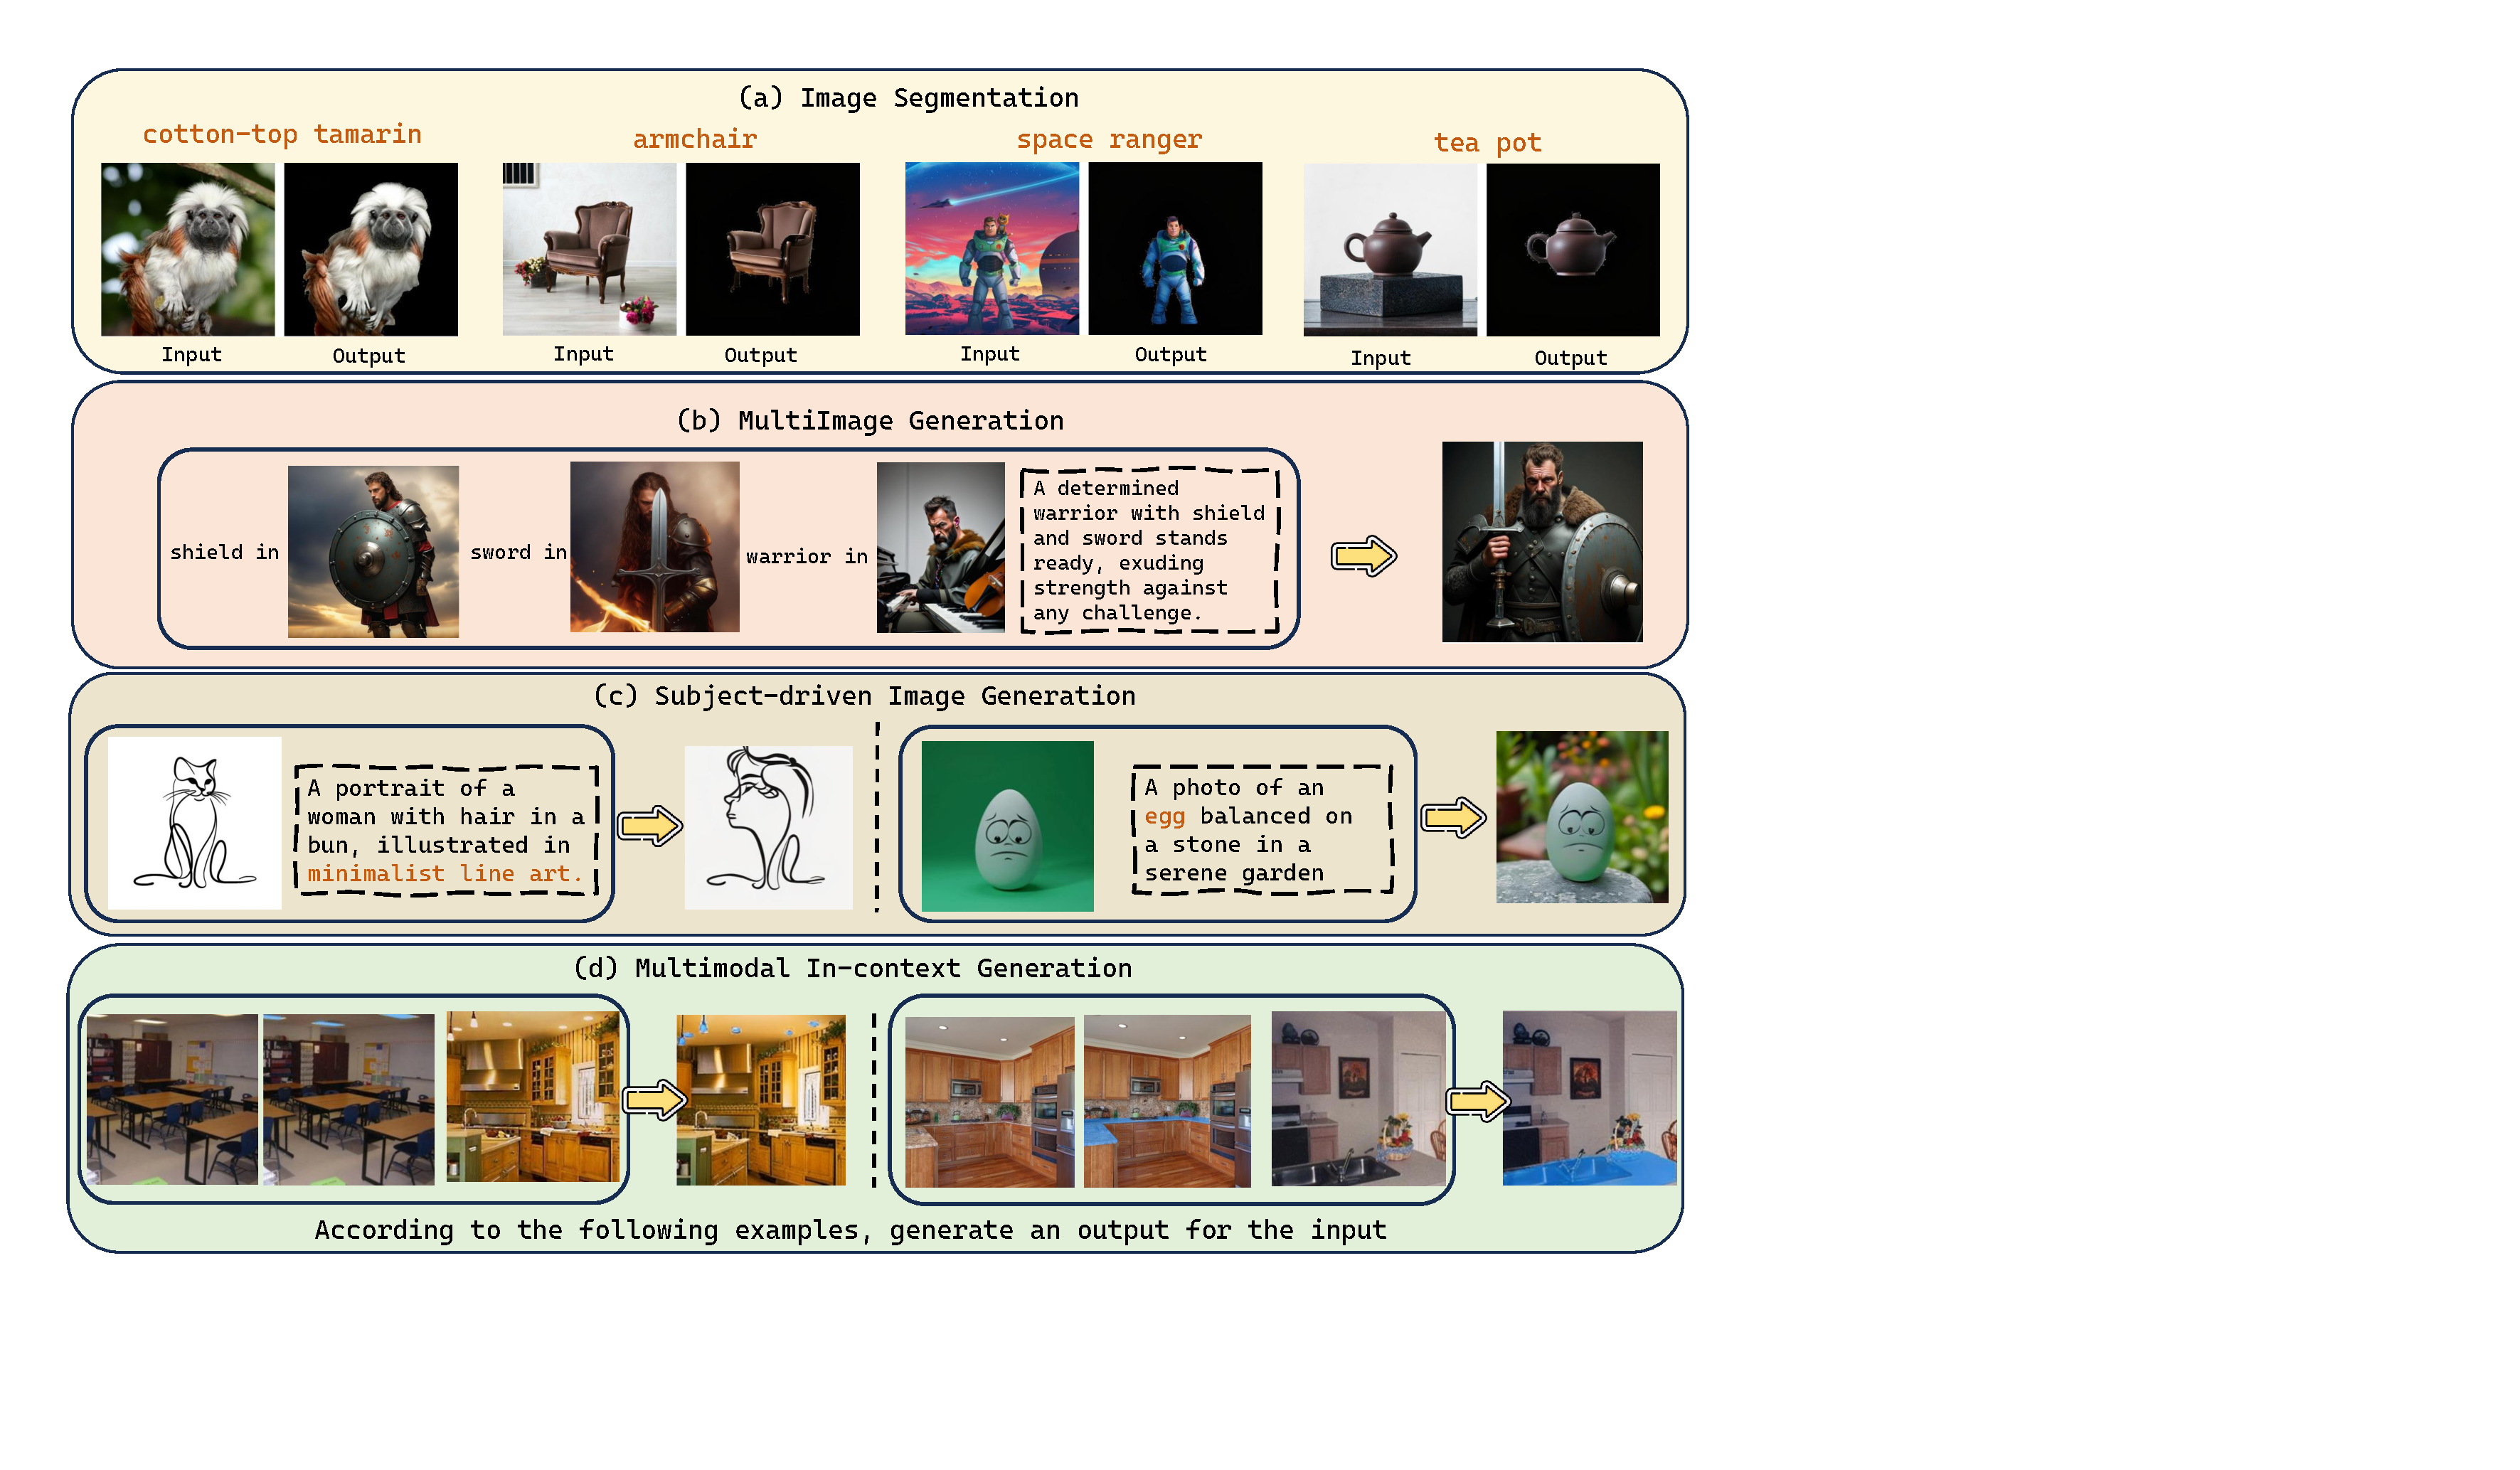
\includegraphics[width=0.7\textwidth]{figures/teasar.pdf}
% 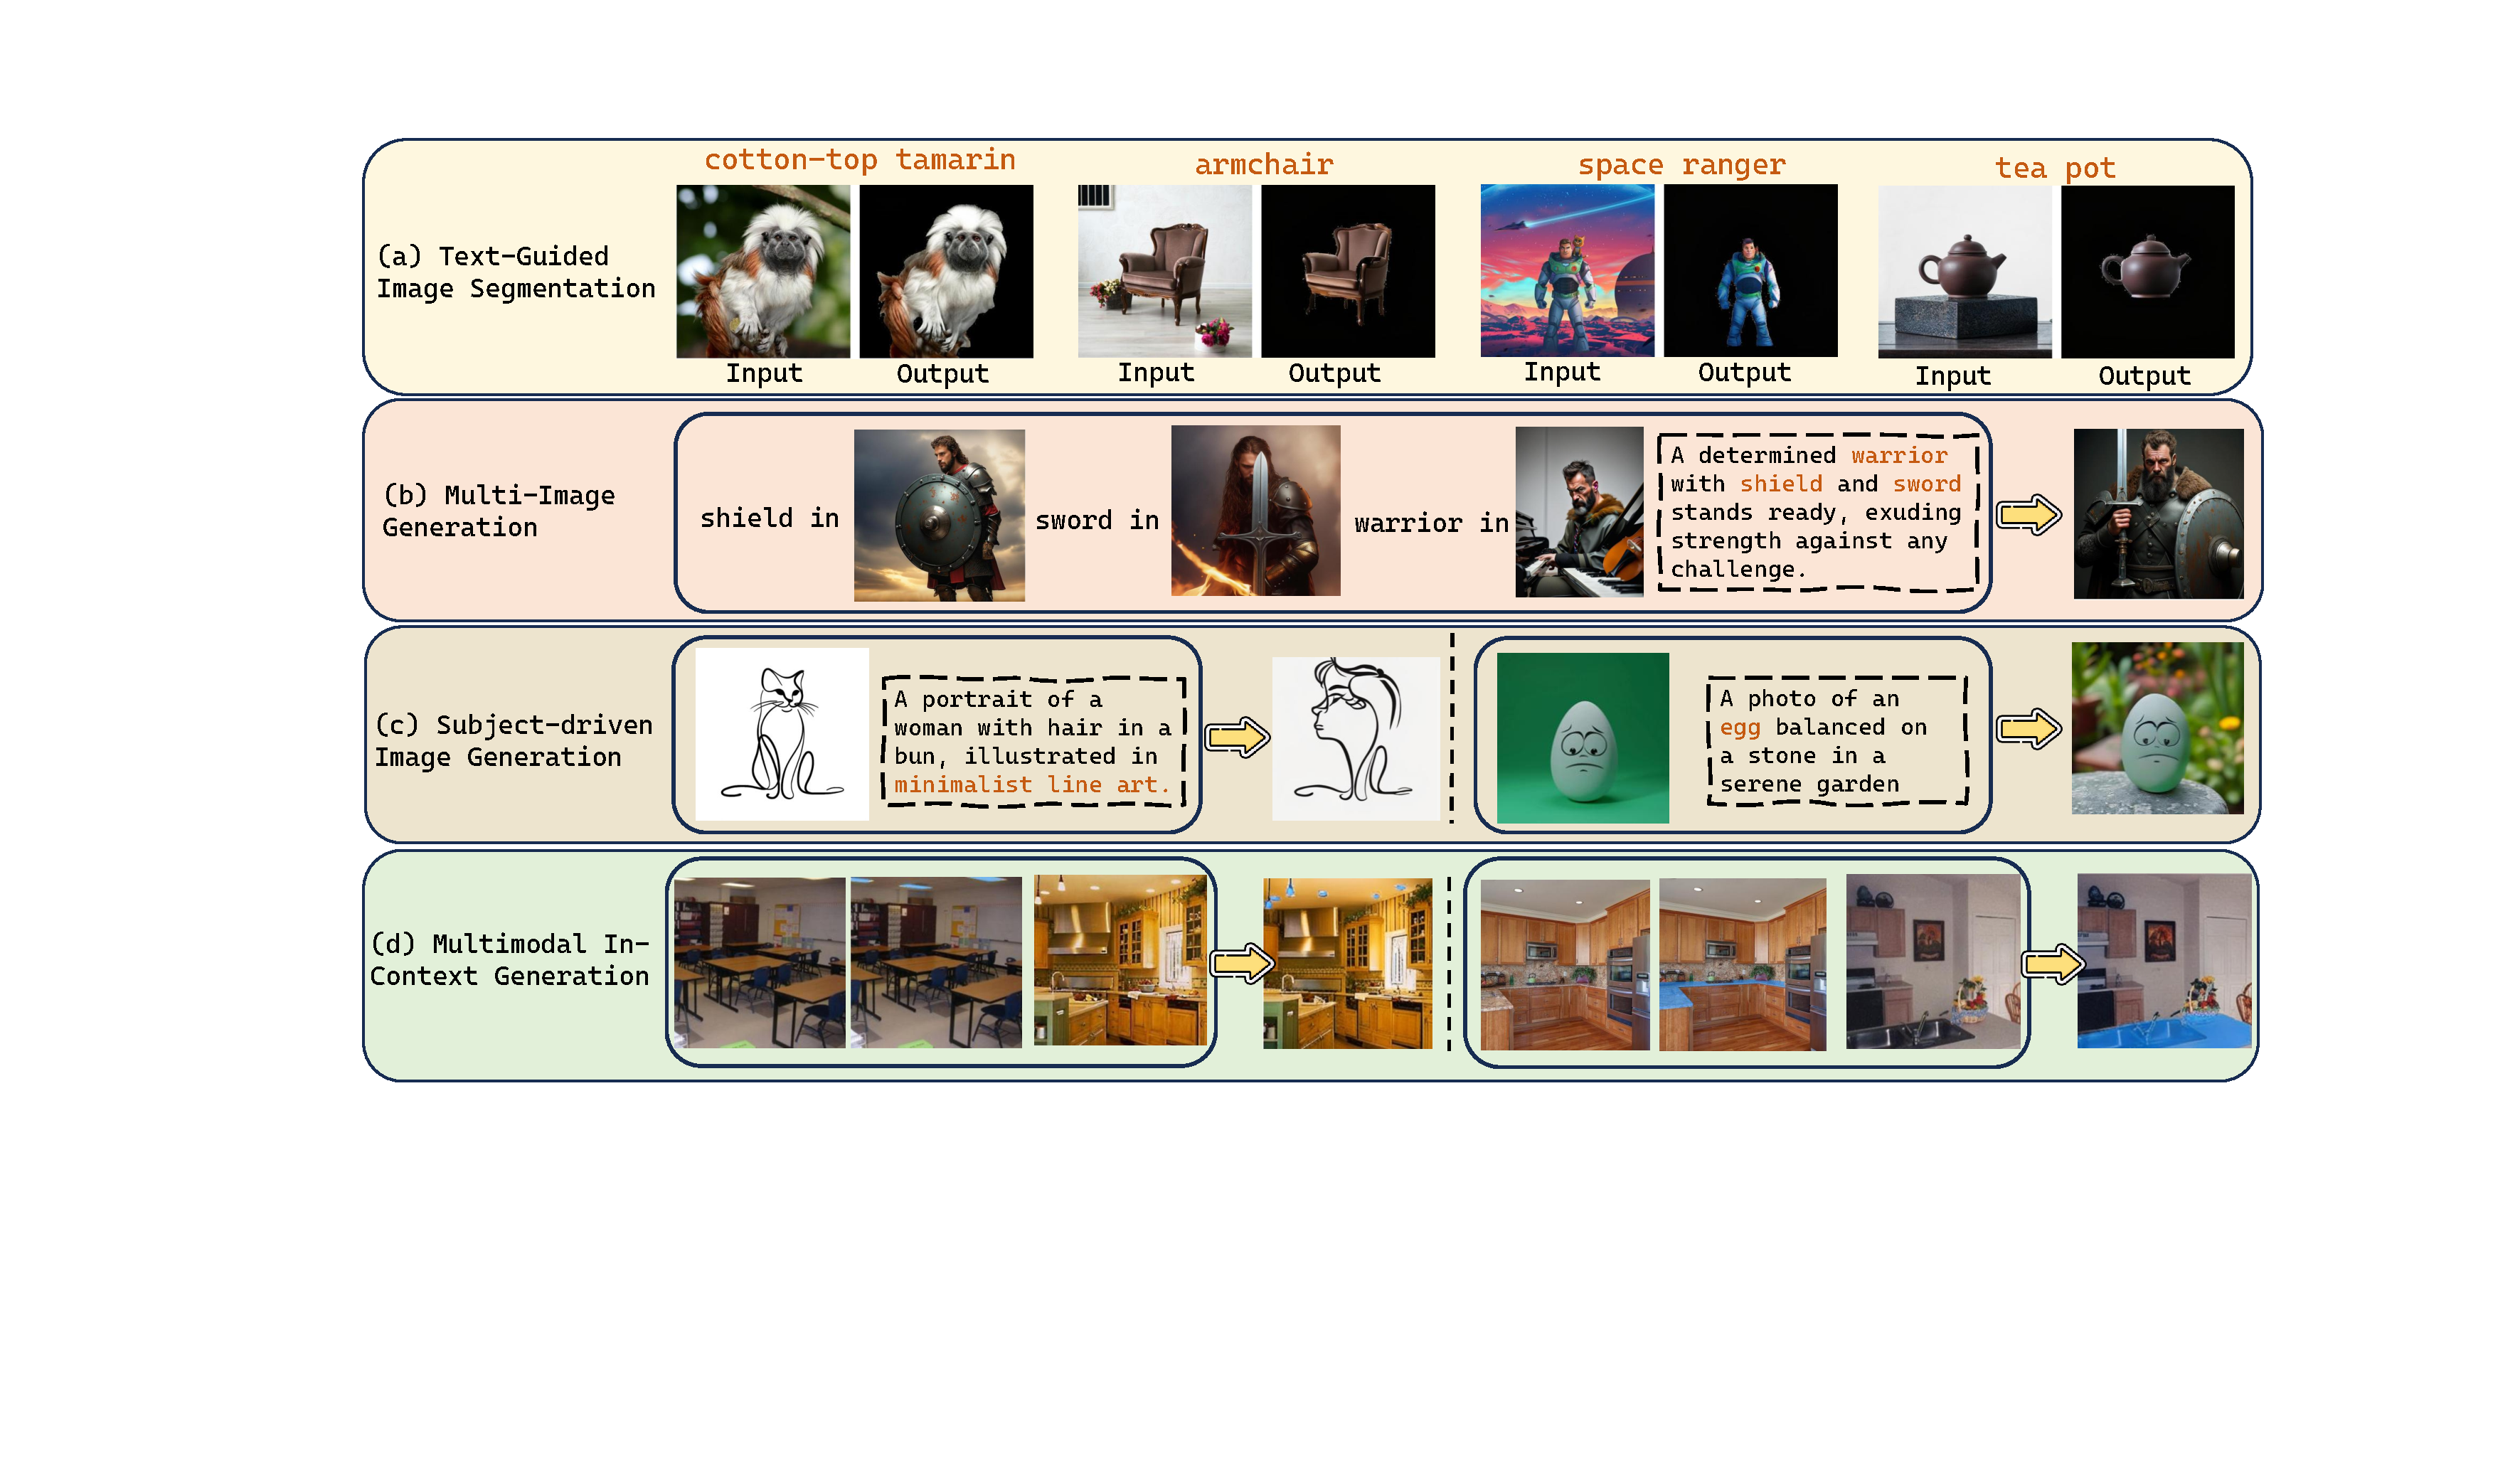
\includegraphics[width=0.9\textwidth]{figures/teasarv2.pdf}
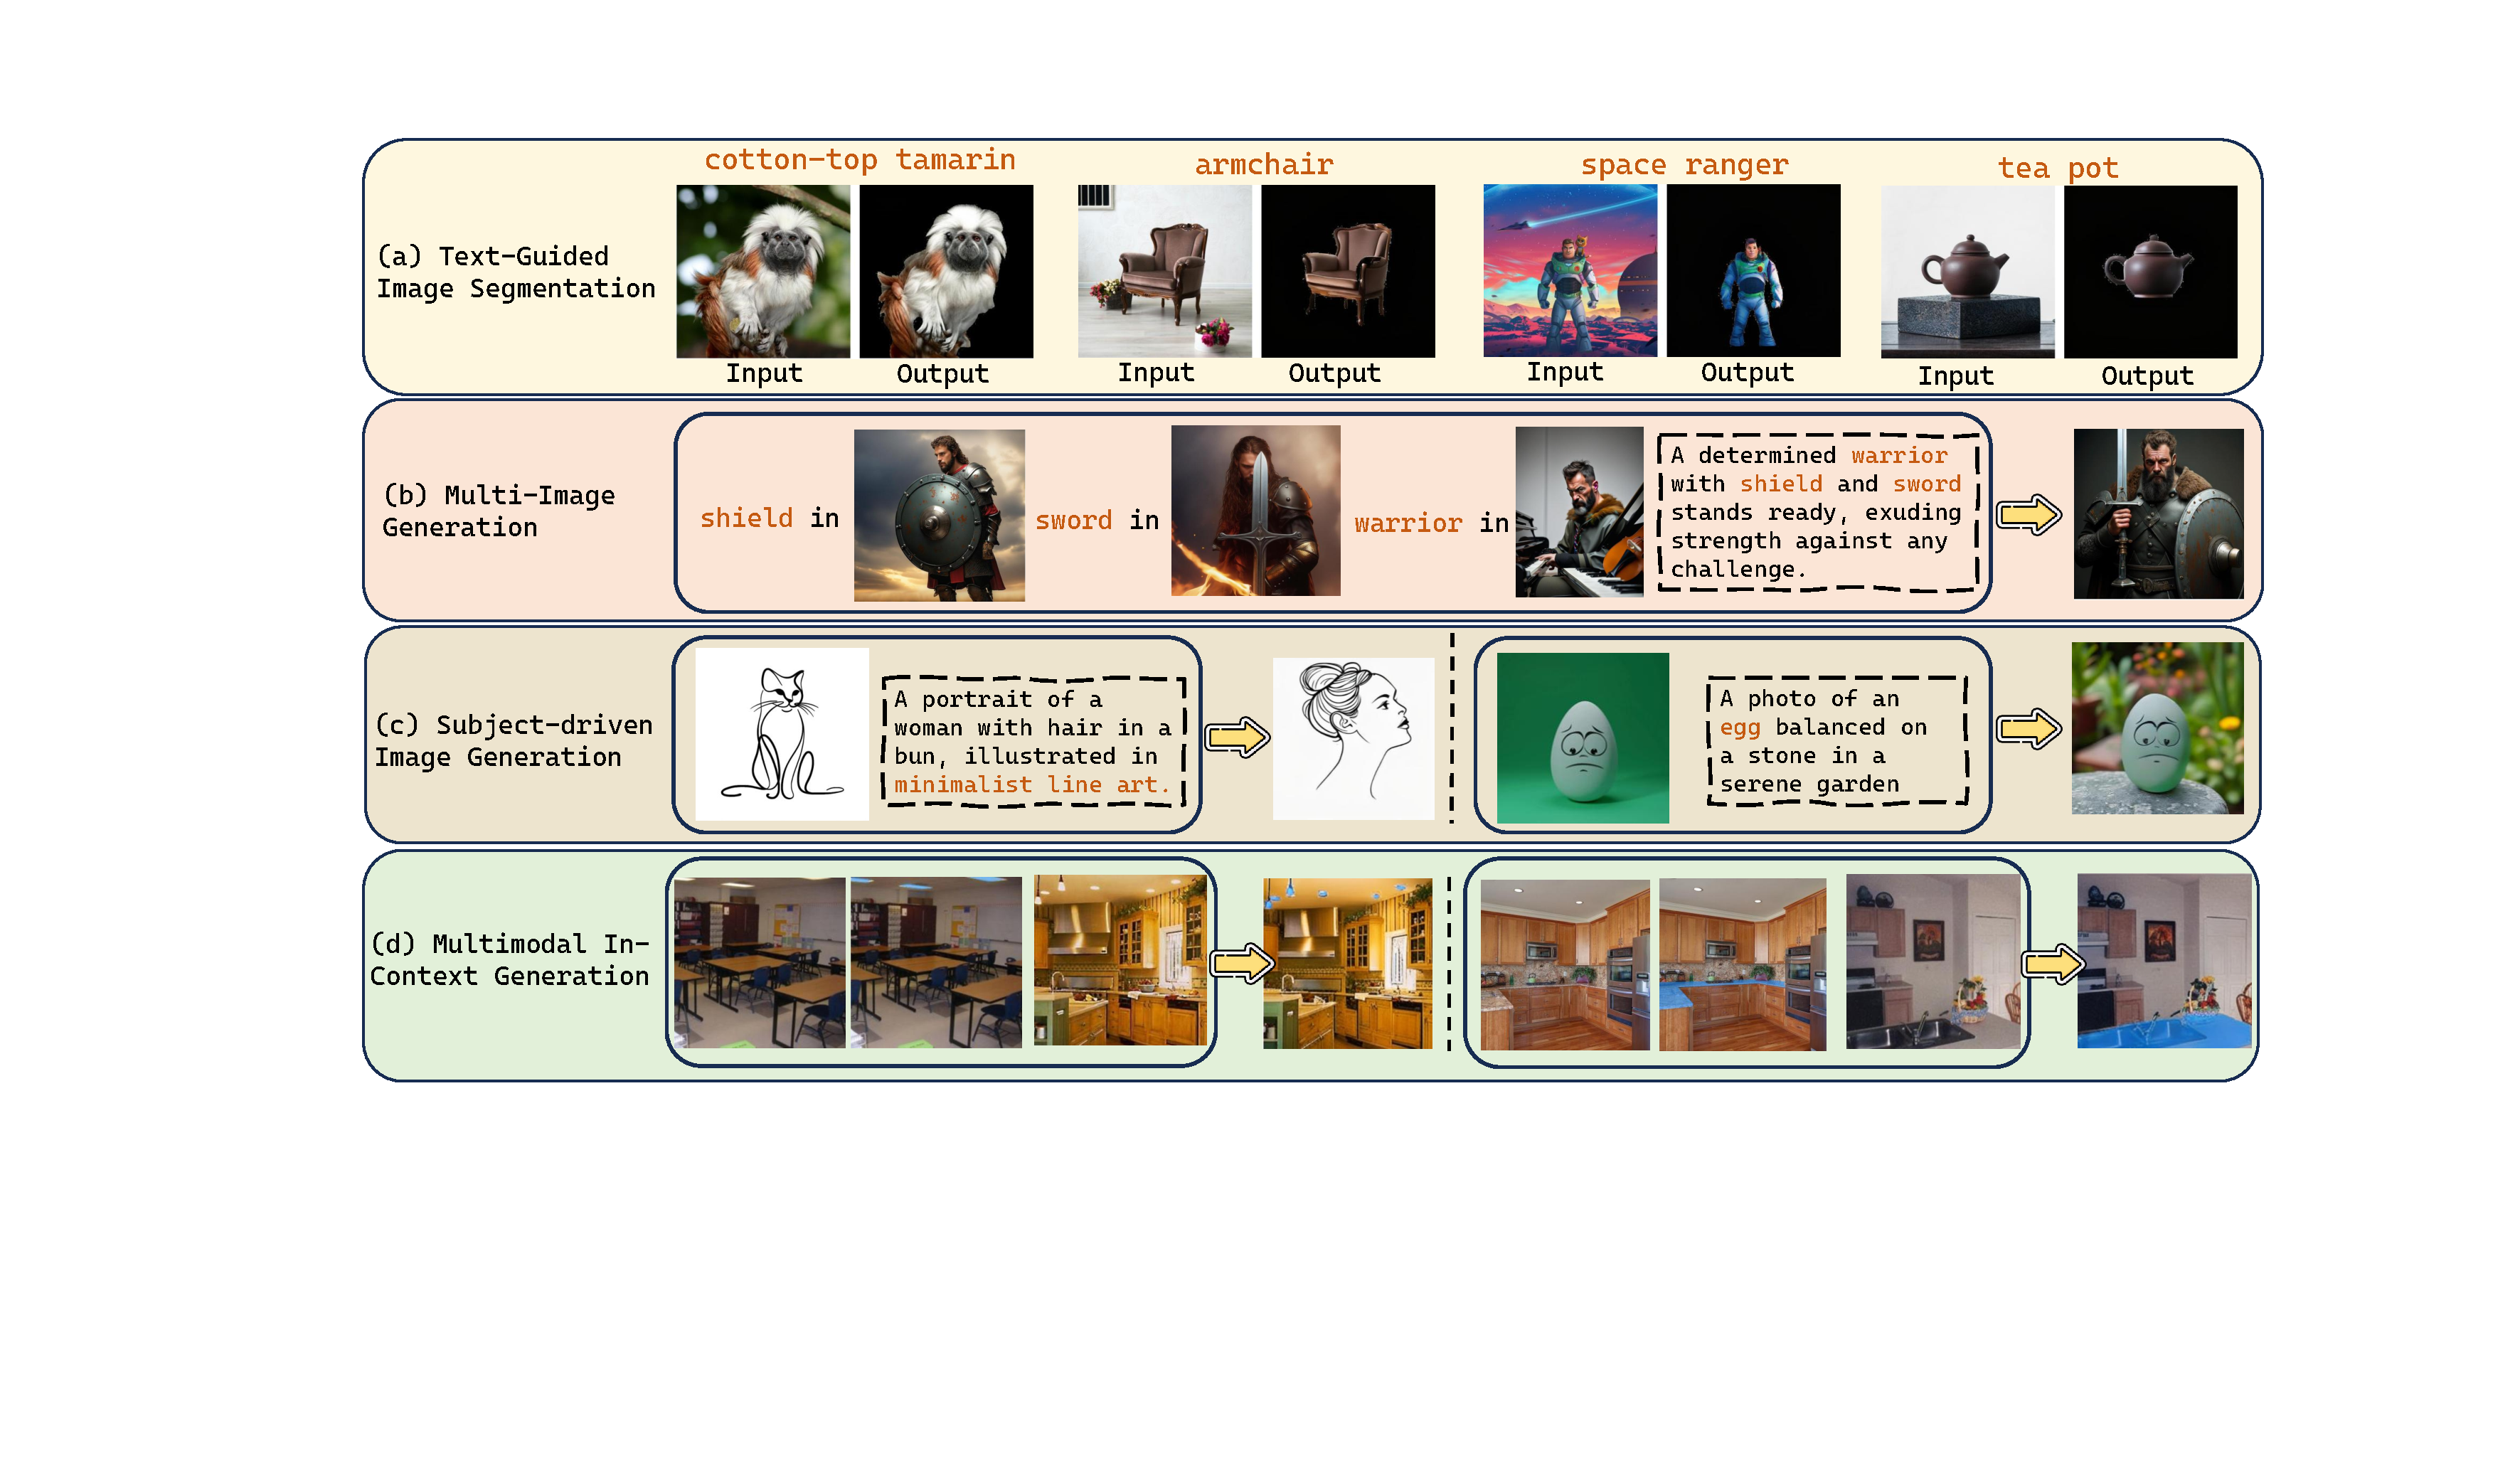
\includegraphics[width=0.9\textwidth]{figures/teasarv3.pdf}
\caption{Versatile applications built on \model after simply fine-tuning on corresponding datasets.
% , including (a) image segmentation, (b) multi-image generation, (c) subject-driven image generation, and (d) multimodal in-context learning image generation
}
\label{fig:examples}
\end{figure*}
\end{abstract}

\section{Introduction} 
\label{sec:introduction}
% \vspace{-1ex}
% \begin{figure}[t]
%     \centering
%     \begin{minipage}{0.45\textwidth}
%         \centering
%         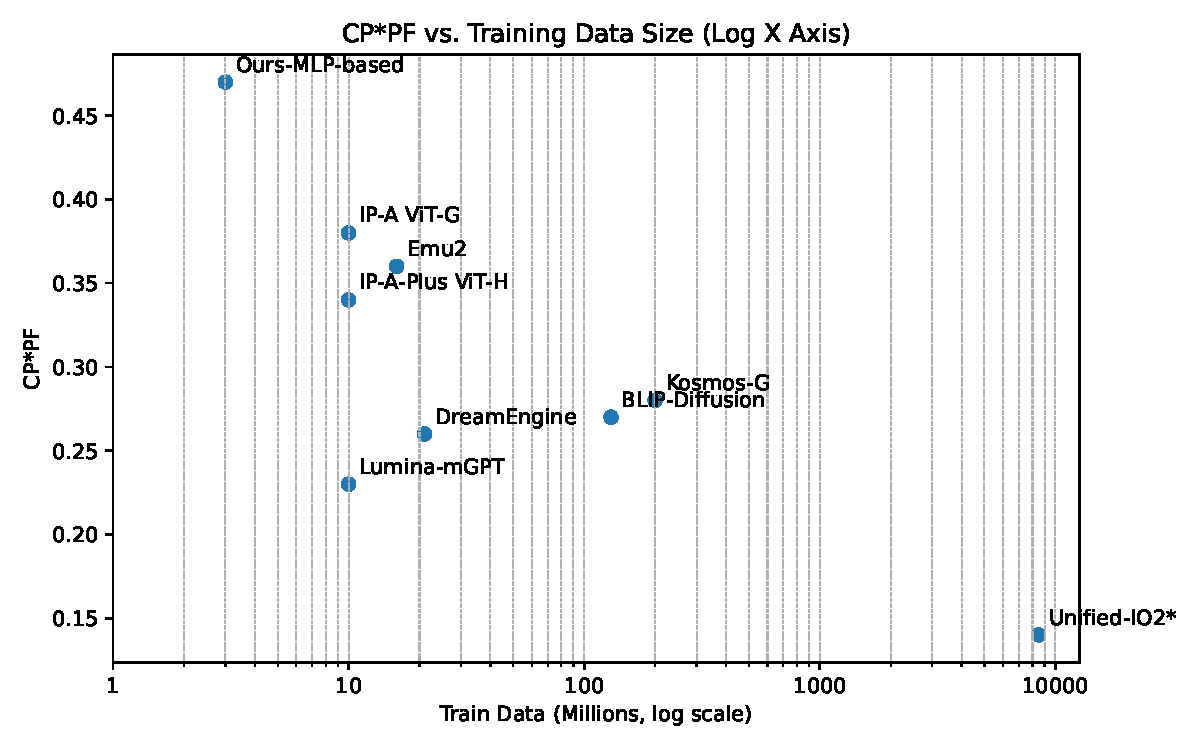
\includegraphics[width=\textwidth]{figures/data.pdf}
%         \caption{data}
%         \label{fig:data}
%     \end{minipage}
%     \hfill
%     \begin{minipage}{0.45\textwidth}
%         \centering
%         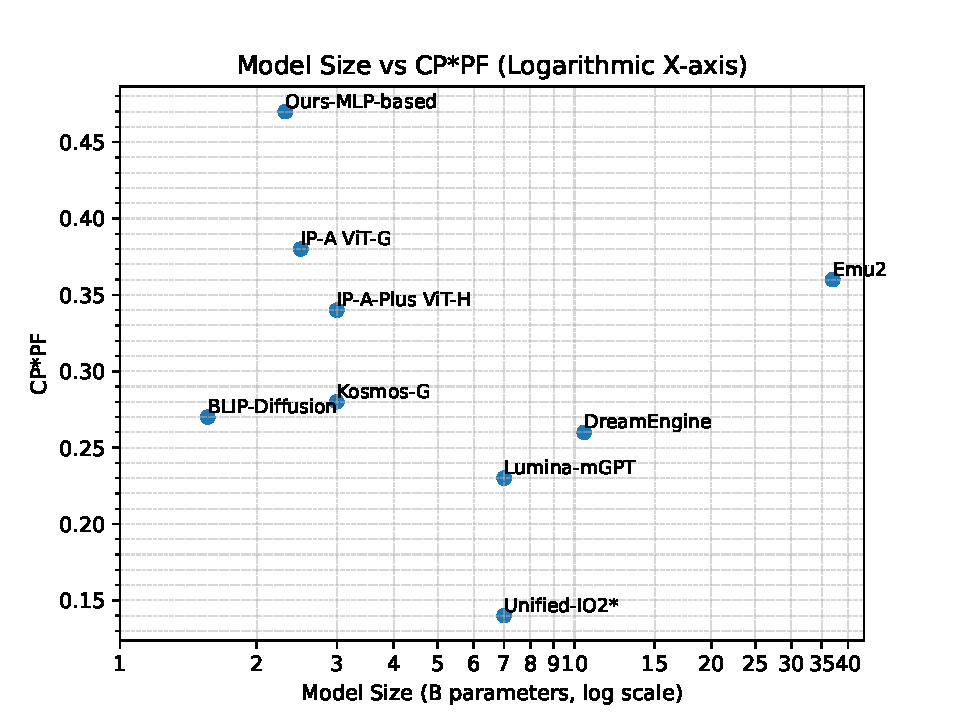
\includegraphics[width=\textwidth]{figures/size.pdf}
%         \caption{size}
%         \label{fig:size}
%     \end{minipage}
%     \caption{Caption text here}
%     \label{fig:comparison}
% \end{figure}

\begin{wrapfigure}{r}{0.50\textwidth} 
    \centering
    \vspace{-5mm}
    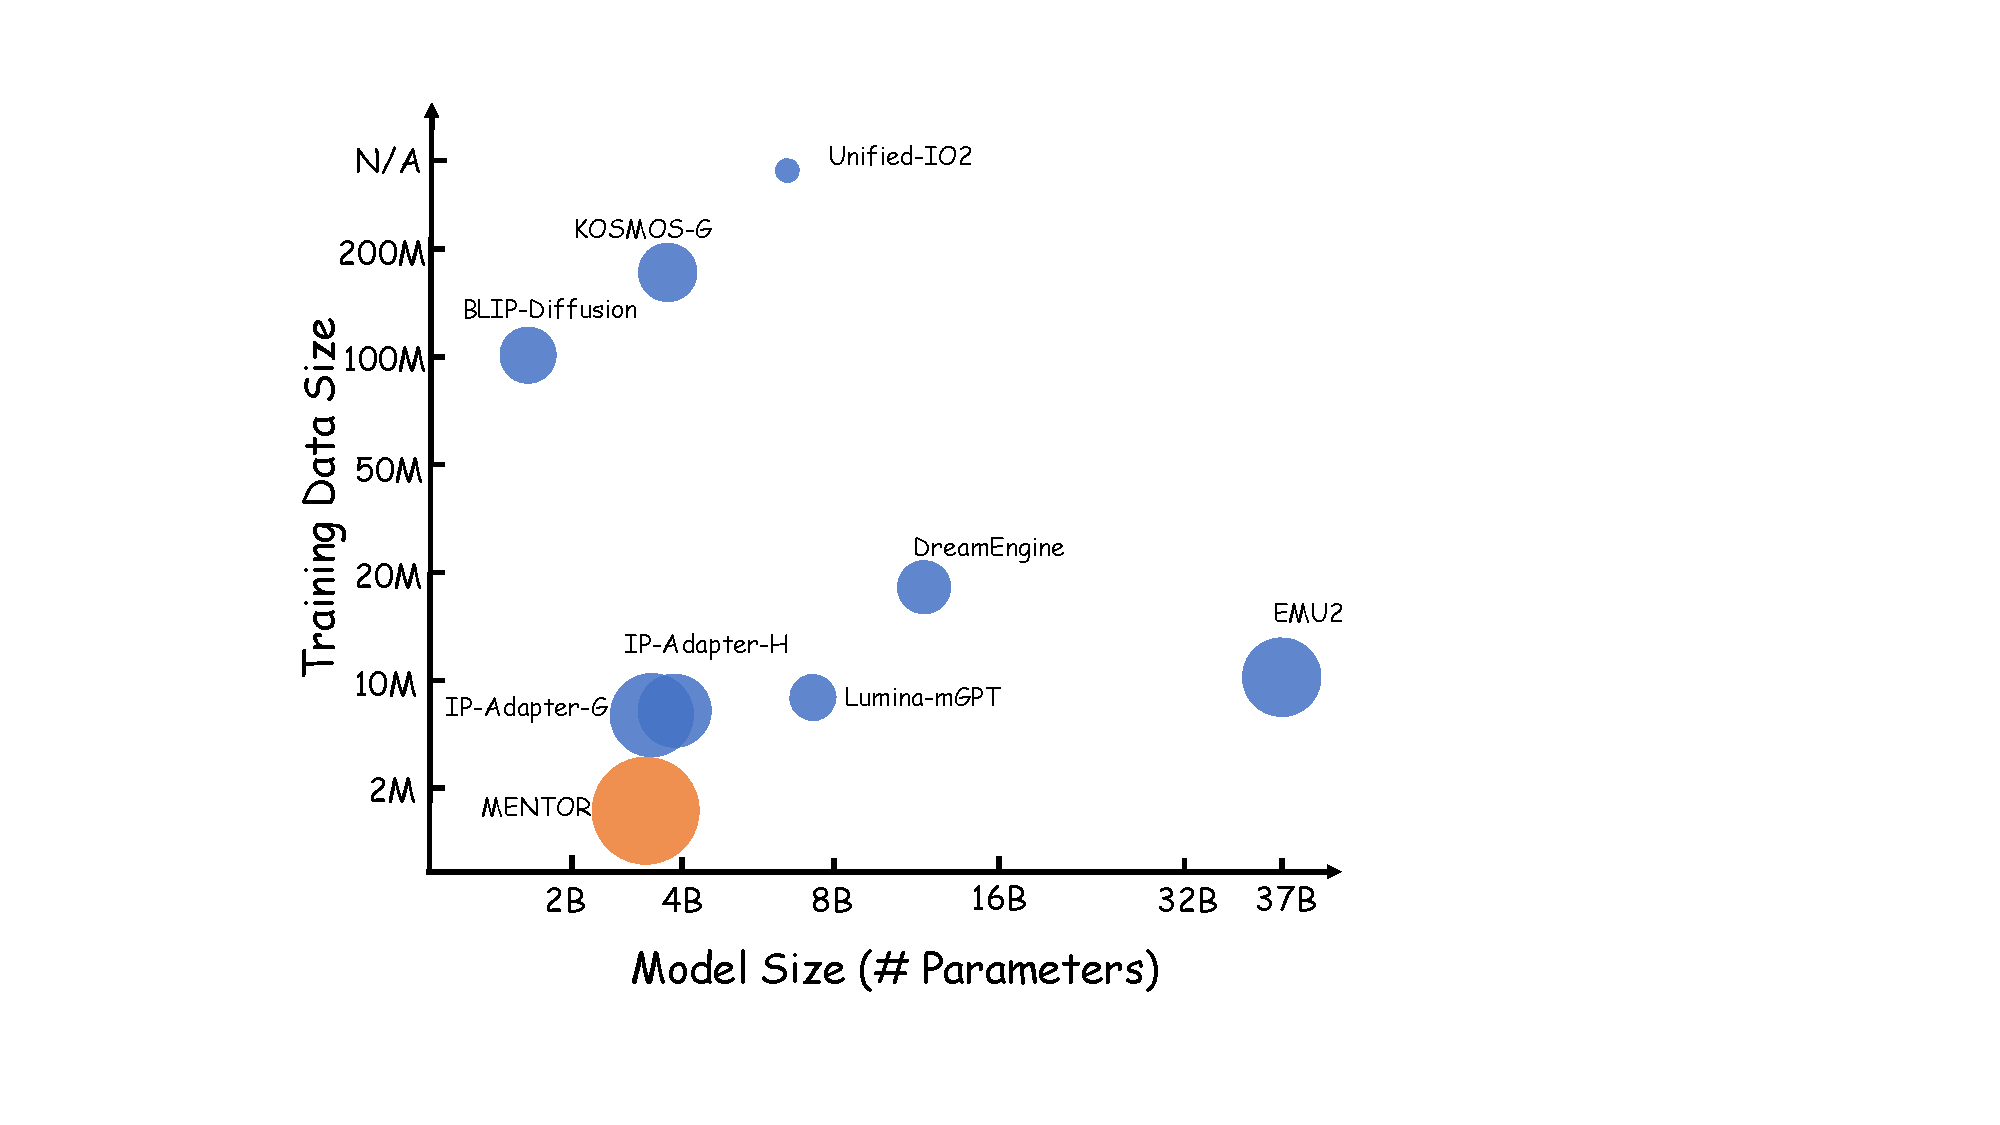
\includegraphics[width=\linewidth]{figures/Figure.pdf}
    % \caption{CP$\cdotp$PF score (circle size) of \model and other baselines on DreamBench++. Model in lower left achieves the best efficiency. }
    \caption{CP$\cdotp$PF score (circle size) of \textcolor[HTML]{ED8B50}{\textbf{\model}} and \textcolor[HTML]{5A76A9}{\textbf{other baselines}} on DreamBench++. Model in lower left achieves the best efficiency.}
    \label{fig:SnapKV}
    \vspace{-0.3cm}
\end{wrapfigure}



Recent progress in generative models has revolutionized text-to-image(T2I) generation~\citep{2020DDPM,ldm,SDXL}. However, real-world applications often require more than text-only prompts.
To achieve high-quality image generation, e.g., fine-grained control over generated images, the models need to seamlessly integrate multi-modal inputs, such as reference images with detailed instructions.
This poses significant challenges for existing diffusion models that are predominantly focused on T2I generation.
To address this, researchers have recently employed Large Multimodal Models (LMMs) to encode diverse inputs into unified embeddings compatible with diffusion models \citep{Kosmos-G, emu2}. While this approach aids in handling complex prompts for generation like interleaved image-text instructions \citep{emu2} or multimodal in-context learning \citep{Kosmos-G,2024SeedX}, several key limitations persist when scaling to complex multimodal control:

% Modern generative models have achieved remarkable success in image generation, with diffusion models leading the state-of-the-art performance in text-to-image generation~\citep{2020DDPM,ldm,SDXL}.
% Recent progress in generative models has revolutionized text-to-image generation with their remarkable capabilities\citep{2020DDPM,ldm,SDXL}.
% Along with their open-source communities, diffusion models dominate the field of visual generation up to today, particularly in text-to-image generation.
% However, real-world image generation applications often demand user interactions beyond simple text-only prompts. 
% To achieve high-quality image generation, e.g., fine-grained control over the generated images, the models need to seamlessly integrate multi-modal inputs, such as reference images, spatial layouts, stylistic exemplars, and detailed textual instructions.
% It poses significant challenges for existing diffusion models that are predominantly focused on text-to-image generation.

% Pervious methods have augmented diffusion models with auxiliary control mechanisms~\citep{controlnet, ye2023ip-adapter,ruiz2023dreamboothfinetuningtexttoimage}, enabling conditional generation guided by additional visual inputs. While effective in specific scenarios, these approaches often rely on task-specific adapters and specialized fine-tuning, which can limit their scalability and broader applicability. 
% Moreover, recent works integrate the large multimodal models (LMMs) with diffusion-based generators~\citep{Kosmos-G, emu2} to encode multimodal inputs into unified embeddings that are compatible with diffusion models, thereby supporting the multimodal conditional image generation.

% To address this challenge, early methods have augmented diffusion models with auxiliary control mechanisms.
% Approaches like ControlNet~\citep{controlnet} and DreamBooth~\citep{ye2023ip-adapter, ruiz2023dreamboothfinetuningtexttoimage} often rely on task-specific adapters and specialized fine-tuning, limiting their generalization ability.
% To address this challenge, more recently, researcher has leveraged Large Multimodal Models (LMMs) to encode diverse multimodal inputs into unified embeddings that are compatible with diffusion models~\citep{Kosmos-G, emu2}. This approach facilitates handling complex multimodal prompts, such as interleaved image-text instructions~\citep{emu2} or multimodal in-context learning~\citep{Kosmos-G,2024SeedX} for image generation.
% Nevertheless, despite their achievements, these methods still face several key limitations when scaled to complex multimodal control:





% To address this challenge, previous methods have augmented diffusion models with auxiliary control mechanisms, such as ControlNet~\citep{controlnet} and IP-Adapter~\citep{ye2023ip-adapter}~\citep{controlnet, ye2023ip-adapter,ruiz2023dreamboothfinetuningtexttoimage}, which often rely on task-specific adapters and specialized fine-tuning. 
% Moreover, others integrate Large Multimodal Models (LMMs) to encode diverse multimodal inputs into unified embeddings that are compatible with diffusion models~\citep{Kosmos-G, emu2}. These method aims to support more complex multimodal prompts, such as interleaved image-text instructions~\citep{emu2} or multimodal in-context learning~\citep{Kosmos-G,2024SeedX} for image generation.
% Despite promising in specific scenarios, these methods still face several key limitations when scaled to complex multimodal control:

% Despite these advances, existing methods still face significant challenges:
% \textbf{First}, the inherent randomness of diffusion processes complicates achieving precise and deterministic control, which is often necessary for tasks requiring high fidelity or accurate image reconstruction~\citep{wang2025imageeditingdiffusionmodels}. 
% \textbf{Second}, effectively balancing guidance of different modalities remains a persistent challenge. 
% Existing methods often struggle to integrate information harmoniously, sometimes over-emphasizing one modality while neglecting others~\citep{han2024emmatexttoimagediffusionmodel}. 
% For instance, methods like IP-Adapter~\citep{ye2023ip-adapter} and Lumina-mGPT~\citep{2024lumina}, which rely on text and image features as conditions, may predominantly be influenced by the image conditions.
% This imbalance can stem from the gap between modalities, which is further exacerbated by model architecture limitations~\citep{zhao2023mmicl,Dig2DIG,ye2023ip-adapter}, as well as suboptimal training paradigms~~\citep{Kosmos-G,han2024emmatexttoimagediffusionmodel}.
% \textbf{Third}, current diffusion-based methods~\citep{Kosmos-G,li2023blipdiffusionpretrainedsubjectrepresentation, emu2}, especially those incorporating auxiliary components for alignment(e.g., learned adapters~\citep{Kosmos-G}, regression heads~\citep{sun2023emu1,emu2}, specialized embeddings~\citep{seed-tokenizer}), typically necessitate extensive training on large-scale datasets~\citep{emu2,Kosmos-G,li2023blipdiffusionpretrainedsubjectrepresentation,2024SeedX}, incurring substantial computational costs.
% This is driven by the large parameter counts of individual components~\citep{emu2,Kosmos-G} (e.g., LLMs, diffusion backbones), auxiliary components, and the need for vast multimodal datasets.

\textbf{First,} the randomness of diffusion processes hinders precise, deterministic control, which is essential for high-fidelity tasks, like image reconstruction\citep{wang2025imageeditingdiffusionmodels}.
\textbf{Second,} balancing guidance from different modalities remains challenging. Existing methods frequently exhibit modality imbalance, often over-emphasizing one modality while neglecting others\citep{han2024emmatexttoimagediffusionmodel}. For instance, IP-Adapter \citep{ye2023ip-adapter} and Lumina-mGPT \citep{2024lumina}, conditioned on text and image features, may overly favor image inputs. This imbalance stems from modality gaps, architectural limitations \citep{zhao2023mmicl,Dig2DIG,ye2023ip-adapter}, or suboptimal training schemes \citep{Kosmos-G,han2024emmatexttoimagediffusionmodel}.
\textbf{Third,} many diffusion-based methods \citep{Kosmos-G, emu2}, particularly those with auxiliary alignment components (e.g., learned adapters \citep{Kosmos-G}, regression heads \citep{sun2023emu1,emu2}, specialized embeddings \citep{seed-tokenizer}), demand large-scale training \citep{emu2,Kosmos-G,li2023blipdiffusionpretrainedsubjectrepresentation,2024SeedX}, incurring substantial computational costs.
These challenges raise a critical question: \textit{Is there a more efficient and controllable paradigm for balancing complex multimodal conditions in image generation?}

% propose \textbf{\model}, a novel autoregressive (AR) framework for efficient \textbf{M}ultimodal g\textbf{E}neratio\textbf{N} \textbf{T}uning for aut\textbf{O}reg\textbf{R}essive multimodal image generation.
To address aforementioned limitations, we propose \textbf{\model}, a straightforward and efficient autoregressive (AR) framework for controllable multimodal image generation. Unlike diffusion models that rely on complex cross-attention layers for multimodal conditioning and demand extensive training resources \citep{2024SeedX,emu2,Kosmos-G,li2023blipdiffusionpretrainedsubjectrepresentation},  \model leverages a unified transformer architecture that directly aligns multimodal inputs with output image tokens. This design inherently simplifies architecture and training, reduces the need for auxiliary components for alignment, and significantly lowers training requirements.
Our framework employs a multimodal encoder to project multimodal inputs into a unified representation. An AR transformer decoder then generates image tokens deterministically, conditioned on this representation. To ensure effective and balanced modality integration, which is curial for multimodal image generation\citep{han2024emmatexttoimagediffusionmodel}, we adopt a two-stage training paradigm: (1) pretraining on image reconstruction and object segmentation to enable robust pixel-level and semantic alignment, followed by (2) multimodal instruction tuning with diverse tasks, such as image recovery and subject-driven generation, explicitly training the model to effectively leverage and balance varied multimodal inputs for coherent generation.

Notably, despite its simplicity and the use of suboptimal checkpoints, \model achieves state-of-the-art(SOTA) performance on the challenging DreamBench++ benchmark—using 10× less training data than leading baselines.
It outperforms resource-intensive baselines with powerful generators like SDXL \citep{SDXL} and SD3 \citep{2024SD3} by 30\% while dramatically reducing computational and data demands. 
Controlled experiments demonstrate the advantages of \model over diffusion-based methods in multimodal fidelity, training efficiency, and generation controllability.


 
% even with readily available multimodal encoders and modestly-sized autoregressive decoders, our method achieves state-of-the-art performance on the challenging DreamBench++ benchmark. It significantly surpasses resource-intensive baselines utilizing powerful generators like SDXL \citep{SDXL} and SD3 \citep{2024SD3} by 30\% while dramatically reducing computational and data demands. Extensive controlled experiments validate our AR approach's compelling advantages in multimodal fidelity, training efficiency, and generation controllability.

% In this paper, we propose a straightforward and efficient autoregressive (AR) framework explicitly designed for controllable multimodal image generation, directly addressing key limitations of prevalent diffusion-based approaches.
% including an AR generation model that suports multimodal conditions and a meticulously designed two-stage training paradigm.
% In contrast to diffusion-based methods that use cross-attention layers for multimodal conditioning and require extensive GPU resources for training, our approach directly aligns multimodal inputs with generated output tokens through unified autoregressive modeling in a simple transformer framework. It facilitates direct, token-level alignment between multimodal conditions and the generated image, providing a direct pathway for integrating diverse inputs.
% This inherent simplicity significantly reduces the reliance on task-specific adapters or extensive auxiliary components, leading to substantially lower training requirements.
% In contrast to diffusion-based methods that employ cross-attention layers for multimodal conditioning and typically necessitate extensive GPU resources for their training phases\citep{2024SeedX,emu2,Kosmos-G,li2023blipdiffusionpretrainedsubjectrepresentation}, our proposed method utilizes unified autoregressive modeling within a transformer architecture. This allows for the direct alignment of multimodal inputs with generated output tokens. 
% Such a direct pathway inherently simplifies the model architecture. 
% Consequently, it reduces the reliance on task-specific adapters or extensive auxiliary components for alignment and has significantly reduced training requirements.


% over diffusion-based counterparts.


% While pervious works like llamaGen~\citep{llamagen}, VILA-U~\citep{VILA-U}, EMU3~\citep{Emu3}, and the Janus-Series~\citep{Janus} have delved into autoregressive text-to-image generation, their capabilities for handling intricate multimodal conditions remain largely unexplored. 
% In contrast, our approach distinctively addresses multimodal conditional generation through the proposed AR framework and a carefully designed two-stage multimodal instruction tuning process. 
% By uniformly handling visual and textual inputs within a sequence-to-sequence modeling framework, our method paves the way towards more efficient, controllable, and robust multimodal generative systems.

% Through this implicit cross-modal alignment, achieved via token-level interactions, our approach substantially reduces the reliance on specialized modality adapters or extensive auxiliary components.
% This inherent simplicity translates directly into significantly reduced training requirements.
% Furthermore, to prevent the model from defaulting to a simple copy-paste function~\citep{han2024emmatexttoimagediffusionmodel} and overlooking textual conditions, our two-stage training process and diverse tasks ensure a nuanced understanding of visual input and a balanced integration of all modalities.


% Our framework utilizes a multimodal encoder to project heterogeneous inputs (visual and textual) into a unified latent space. An autoregressive transformer decoder then deterministically generates image tokens based on this unified representation. 
% To ensure robust understanding and balanced integration of diverse modalities—specifically preventing the model from defaulting to simple copy-paste function~\citep{han2024emmatexttoimagediffusionmodel} while ignoring textual instructions—we introduce a carefully designed two-stage training paradigm. In the first stage, the model is pretrained on image reconstruction and object segmentation tasks, fostering robust pixel-level and semantic-level alignment between the multimodal input and generated tokens. Subsequently, the second stage involves multimodal instruction tuning with diverse tasks, such as image recovery and subject-driven generation. This stage explicitly trains the model to leverage varied multimodal inputs effectively while balancing its focus across different modalities for coherent image generation.



% Specifically, our method employs a multimodal encoder to project heterogeneous inputs—visual and textual data—into a unified latent embedding space, creating a comprehensive multimodal representation. An autoregressive transformer-based decoder subsequently generates images based on this representation, producing deterministic outputs that accurately reflect the provided conditions.
% Building upon this architecture, we introduce a meticulously designed two-stage training paradigm. In the first stage, the model is pretrained on image reconstruction and object segmentation tasks, fostering robust pixel-level and semantic-level alignment and encouraging effective exploitation of visual information for image synthesis. 
% Subsequently, we perform the multimodal instruction tuning that incorporates additional training tasks, such as image recovery and subject-driven image generation. The second stage empowers the model to leverage varied multimodal inputs for image generation while explicitly balancing its focus across different modalities, enabling an efficient and robust fusion of multimodal information into coherent image outputs.

% Remarkably, even when employing readily available multimodal encoders and modestly-sized autoregressive decoders, our method achieves state-of-the-art performance on the challenging DreamBench++ benchmark. It surpasses the resource-intensive baselines, which utilize much more power generators like SDXL~\citep{SDXL} and SD3~\citep{2024SD3}, by xx\% while dramatically reducing computational and data resource demands. Through extensive controlled experiments, we directly compare our AR approach with diffusion-based counterparts and demonstrate compelling advantages in multimodal fidelity, training efficiency, and generation controllability.

% our method surpasses other baselines and achieves state-of-the-art performance on the challenging DreamBench++ benchmark by xx\%, while dramatically reducing computational and data resource demands. We also conduct extensive controlled experiments comparing our autoregressive approach directly with diffusion-based paradigms. 
% Our findings demonstrate that autoregressive models offer significant advantages in multimodal fidelity, generation controllability, and consistency.


% Our contributions are summarized as follows:
% \begin{itemize}[left=2pt]
% \item We propose a novel autoregressive framework for efficient multimodal image generation tuning, demonstrating state-of-the-art performance with substantially reduced training resources.
% \item We introduce a two-stage training strategy to align multimodal embeddings effectively, enabling balanced multimodal attention and precise conditional adherence.
% \item Extensive experiments validate the superior efficiency and multimodal capabilities of our AR framework, highlighting its potential as a scalable alternative to existing diffusion-based methods.
% \end{itemize}
Overall, our contributions are as follows: (1) A novel autoregressive framework for efficient multimodal generation, achieving, achieving SOTA performance; (2) A two-stage training strategy for multimodal-conditioned tuning, enabling robust alignment and balanced modality integration with significantly reduced training cost; (3) Extensive experiments demonstrating the superior efficiency, controllability, and fidelity of \model as a compelling alternative to diffusion-based methods.



% Our contributions are:
% \begin{itemize}[left=2pt]
%     % \setlength\itemsep{0.1em}
%     \item A novel autoregressive framework for efficient and controllable multimodal  generation, achieving state-of-the-art performance with substantially reduced training resources.
%     \item A two-stage training strategy to ensure robust multimodal alignment and balanced integration of diverse modalities for controllable multimodal image generation.
%     \item Extensive experiments validating the superior efficiency, controllability and multimodal fidelity of \model, highlighting its potential as a scalable alternative to the diffusion-based methods.
% \end{itemize}



% The proposed model integrates a multimodal encoder with a unified transformer decoder. The multimodal encoder is responsible for processing and fusing multimodal inputs into a coherent conditioning representation. It converts each input into combined latent token sequence for generation. This encoded sequence of tokens serves as deterministic context for the decoder. The unified transformer decoder then autoregressively generates the output image token-by-token. 

% Thanks to this design, our model can seamlessly integrate information from multimodal conditions and synthesize a new image that precisely reflects all these inputs, leading to three key advantages:

% \begin{itemize} 
% \item \textbf{Deterministic Control.} The absence of stochastic sampling enables consistent and interpretable outputs, supporting precise image reconstruction and fine-grained editing.
% \item \textbf{Multimodal Instruction Following.} Both language and vision are treated uniformly as token sequences, enabling seamless cross-modal attention and better instruction following for image generation. 
% \item \textbf{Training Efficiency.} Unified autoregressive modeling facilitates the direct alignment of multimodal inputs with output sequences. This implicit shortcut reduces reliance on modality-specific alignment modules, and also significantly lowers training costs.
% \end{itemize}



% Our AR model achieves state-of-the-art performance on the DreamBench++ benchmark, outperforming prior diffusion-based methods. Notably, our approach attains this strong performance with far fewer resources. In fact, even with sub-optimal large multimodal modules as the encoder and a relatively low-capacity image decoder, our AR framework matches surpasses other baselines. This highlights the training efficiency and effectiveness of our proposed paradigm – by treating generation as a discrete sequence prediction, we sidestep the need for large training data and lengthy training schedules, yet still capture the complex relationships between multimodal inputs and outputs.

% Furthermore, we conduct extensive controlled experiments to directly compare the AR and diffusion paradigms in multimodal conditional generation scenarios
% Our findings reveal that autoregressive models offer a promising and underexplored alternative for conditional image generation, particularly in multimodal settings requiring fine-grained control and interpretability. By unifying visual and text inputs in a sequence-to-sequence formulation, our approach paves the way toward more controllable and efficient generative systems.



% efficiency : model size training data

% \section{Preliminary}
\label{sec:preliminary}

\subsection{Model Design}


\section{Method}
\label{sec:method}


% This section details our proposed autoregressive framework for multimodal conditional image generation, its core components, two-stage training paradigm, and the data construction pipeline. 
This section details an efficient autoregressive framework for controllable multimodal image generation, achieving precise image control and balancing guidance across multiple modalities with minimal cost.
\Cref{sec:Preliminary} describes the autoregressive training objective for our framework. Next, \Cref{sec:model} presents a straightforward yet efficient model architecture, detailing how the framework accommodates multimodal inputs and supports autoregressive generation.
Crucially, \Cref{sec:traing_stages} introduces a two-stage training paradigm aimed at balancing the influences of different modalities during image generation.
Finally, \Cref{sec:data_construct} describes our automated pipeline for scalable multimodal data curation.

\subsection{Preliminary}
\label{sec:Preliminary}
\textbf{Training Objective}
Our model employs \emph{teacher forcing} to predict image tokens, conditioned on (i) previously generated tokens and (ii) multimodal context $\mathbf{h}$. 
Given the multimodal condition: $\mathbf{c}^{(0)} = \{\mathcal{I}, \mathcal{T}\}$ (visual and textual inputs),
a multimodal encoder~\(\phi\) first encodes $\mathbf{c}^{(0)}$ and subsequently uses an MLP layer to project them into space of the image decoder to form a unified representation $\mathbf{h}$:
\begin{equation}
    \mathbf{H} = \text{MLP}(\phi\bigl(\mathbf{c}^{(0)}\bigr))
    = (\mathbf{h}_1, \dots, \mathbf{h}_{M}) \in \mathbb{R}^{M\times d}, \qquad \mathbf{h}_j \in \mathbb{R}^{d}.
    \label{eq:enc}
\end{equation}
where $M$ is the number of conditioning tokens, and $d$ is the dimension of the latent embeddings.
% The autoregressive decoder $\theta$, conditioned on $\mathbf{h}$, generates an image token sequence $\mathbf{y} = (y_1, \dots, y_{L})$ of length $L$. Its conditional distribution factorizes as:
Then, the AR decoder $\theta$, conditioned on $\mathbf{h}$, generates image sequence $\mathbf{y} = (y_1, \dots, y_L)$ as follows:
\begin{equation}
    \small
    \theta(\mathbf{y} \mid \mathbf{H}) = \prod_{i=1}^{L} \theta\bigl(y_i \mid y_{<i}, \mathbf{H}\bigr).
    \label{eq:factor}
\end{equation}
% where $y_{<i} = (y_1, \dots, y_{i-1})$ are the preceding tokens.
The training objective is to minimize the token-level cross-entropy loss by \emph{teacher forcing} on data $\mathcal{D}$:
\begin{equation}
\small
    \mathcal{L}_{\text{CE}}(\theta, \phi)
    = -\mathbb{E}_{(\mathbf{y}, \mathbf{c}^{(0)}) \sim \mathcal{D}}
    \left[
        \sum_{i=1}^{L}
        \log \theta\bigl(y_i \mid y_{<i}, \mathbf{H} \bigr)
    \right].
    \label{eq:ce}
\end{equation}
% Our model is trained using \emph{teacher forcing} to predict image tokens, conditioned on (i) previously generated tokens and (ii) multimodal context provided by multimodal encoder.

% Formally, given the initial multimodal condition: $\mathbf{c}^{(0)} = \{\mathcal{I}, \mathcal{T}\}$, where $\mathcal{I}$ and $\mathcal{T}$ represent visual and textual inputs, respectively. To transform the multimodal inputs $\mathbf{c}^{(0)}$ into a unified representation $\mathbf{h}$, the multimodal encoder~\(\phi\) first encodes the input into conditioning hidden states and subsequently projects them into the latent embedding space of the decoder via a MLP projection layer:

% \begin{equation}
%    \mathbf{h} = \text{MLP}(\phi\bigl(\mathbf{c}^{(0)}\bigr))
%    = (h_1, \dots, h_{M}), \qquad h_j \in \mathbb{R}^{d},
%    \label{eq:enc}
% \end{equation}
% where $M$ is the number of conditioning tokens, and $d$ is the dimensionality of the latent embeddings. 

% The autoregressive decoder $\theta$ receives the sequence $\mathbf{h}$ as a prefix and generates an output sequence of image tokens $\mathbf{y} = (y_1, \dots, y_{L})$, where $L$ is the length of the target image-token sequence. The conditional distribution modeled by the decoder factorizes autoregressively as:
% \begin{equation}
%    \theta(\mathbf{y} \mid \mathbf{h})
%    = \prod_{i=1}^{L}
%    \theta\bigl(y_i \mid y_{<i}, \mathbf{h}\bigr),
%    \label{eq:factor}
% \end{equation}
% where $y_{<i} = (y_1, \dots, y_{i-1})$ denotes the previously generated tokens.

% Training is performed using \emph{teacher forcing}, where ground-truth prefix tokens are provided at each step. The objective is to minimize the token-level cross-entropy loss over the data distribution $\mathcal{D}$:
% \begin{equation}
%    \mathcal{L}_{\text{CE}}(\theta, \phi)
%    = -\mathbb{E}_{(\mathbf{y}, \mathbf{c}^{(0)}) \sim \mathcal{D}}
%    \left[
%       \sum_{i=1}^{L}
%       \log \theta\bigl(y_i \mid y_{<i}, \phi(\mathbf{c}^{(0)})\bigr)
%    \right].
%    \label{eq:ce}
% \end{equation}
\textbf{Classifier-free Guidance} 
To enhance multimodal generation controllability, we apply Classifier-Free Guidance (CFG)~\citep{llamagen}. During training, multimodal conditioning \(\mathbf{H}\) is replaced by a learned unconditional embedding \(\mathbf{H}_u\) with probability \(p\). At inference time, token logits \(\ell_g\) are recalculated by interpolating between the conditional logits \(\ell_c\) (from \(\mathbf{H}\)) and unconditional logits \(\ell_u\) (from \(\mathbf{H}_u\)), controlled by a scaling parameter \(\lambda\):
\(\ell_g = \ell_u + (\ell_c - \ell_u) \times \lambda\).





% To enhance the multimodal conditional generation capabilities of the model, following pervious methods~\citep{llamagen}, we integrate \emph{classifier-free guidance} (CFG) during both training and inference phases. 
% Specifically, during training, we randomly replace the original multimodal inputs $c$ with learnable conditional embeddings $u$ with the possibility $p$. 
% % to encourage the model to generalize beyond strict reliance on provided conditions. 
% At inference time, the logits for each predicted token are recalculated by interpolating between the conditional logits $\ell_{c}$ obtained from original multimodal conditions $c$ and unconditional logits $\ell_{u}$ derived from the learned conditional embeddings $u$, controlled by a scaling parameter $\lambda$:
% \begin{equation}  
% \ell_{g} = \ell_{u} + (\ell_{c} - \ell_{u}) \times \lambda.
% \end{equation}  

% To enhance the controllability and guidance strength of multimodal generation, we integrate Classifier-Free Guidance (CFG) for multimodal conditional generation following pervious methods~\citep{llamagen}.
% During training, we randomly drop the multimodal conditions (e.g., replacing $\mathbf{h}$ with a learned unconditional embedding $\mathbf{h}_u$) with a certain probability $p$. 
% At inference time, the logits for the next token prediction are computed by interpolating between the conditional logits $\ell_c$ and unconditional logits $\ell_u$ using a guidance scale parameter $\lambda$:
% \begin{equation}
% \ell_{g} = \ell_{u} + (\ell_{c} - \ell_{u}) \times \lambda,
% \label{eq:cfg}
% \end{equation}
% where $\ell_c$ are derived from the model conditioned on the full multimodal input $\mathbf{h}$, $\ell_u$ are derived from the model conditioned on the learned unconditional embedding $\mathbf{h}_u$.


% Through this formulation, CFG provides flexible control over conditional strength, enabling the model to achieve a balance between coherence and diversity in the generated outputs.


\subsection{Model Design}
\label{sec:model}
As illustrated in \Cref{fig:structure}, \model architecture comprises two core components: a multimodal encoder and an autoregressive generation decoder. These components are designed to unify multimodal inputs into a shared embedding and generate image tokens sequentially conditioned on the unified embedding, respectively. 
A lightweight projection layer bridges the encoder's output to the decoder's input embedding space, enabling seamless integration between the two components.
% The multimodal encoder is responsible for unifying heterogeneous modalities (e.g., text and vision) into a shared latent space, providing conditional signals to guide the autoregressive image generator. These components are bridged via a lightweight multi-layer perceptron (MLP) projection layer, enabling seamless integration between the encoder’s output and the decoder’s input embedding space.


\textbf{Multimodal Encoder}
The multimodal encoder integrates multimodal inputs from frozen pretrained vision ($\phi_V$) and language ($\phi_L$) encoders into a shared latent space. This module projects visual features from $\phi_V$ into $\phi_L$'s embedding space using a lightweight connector module ($\psi$), yielding a unified multimodal representation $\mathbf{H} = (\mathbf{h}_1, \dots, \mathbf{h}_{M})$, where $\mathbf{h}_j \in \mathbb{R}^{d}$. 
% To address the computational demands of extensive visual tokens from $\phi_V$ while preserving detail, two architectures for $\psi$ are investigated:
Meanwhile, a critical challenge arises from the visual tokenization, where a vision encoder produces hundreds of tokens per image. It inflates the context length and leads to substantial computational costs, especially in multi-image scenarios. Compressing visual tokens can mitigate costs,  but may risk losing fine-grained visual information. To navigate this trade-off, two architectures for $\psi$ are investigated:

\begin{itemize}[left=2pt, itemsep=0.5pt,topsep=0.5pt]
    \item \textbf{MLP-based Projection}: Inspired by~\cite{liu2023llava}, we adopt a multi-layer perceptron that directly projects visual tokens to maintain detailed visual semantics with minimal information loss.
\item \textbf{Query-based Token Distillation}: We use a Query-Former~\cite{li2023blip2} to compress lengthy visual token sequences into a fixed-size representation. To guide the distillation, we condition the Query-Former on textual queries\citep{li2023blipdiffusionpretrainedsubjectrepresentation,2023instructblip} that highlight important concepts in images. It aims to guide the model to selectively extract semantically relevant visual features based on textual queries.
\end{itemize}

% The resulting multimodal encoder serves as the foundation for subsequent image generation.

% The multimodal encoder is designed to integrate vision and language inputs into a shared latent space that serves as the conditional input for the decoder. It is constructed by combining a frozen vision encoder($\phi_V$) and a frozen language model encoder ($\phi_L$), connected via a lightweight connector module ($\psi$). This connector is trained to project the features from the vision encoder into the language model's embedding space, yielding a unified multimodal representation $\mathbf{h}$.

% The multimodal encoder integrates vision ($\phi_V$) and language ($\phi_L$) inputs—both processed by frozen pretrained encoders—into a shared latent space. A lightweight connector module ($\psi$) projects visual features from $\phi_V$ into the embedding space of $\phi_L$, yielding a unified multimodal representation $\mathbf{h}$.

% To manage the computational burden of extensive visual tokens from $\phi_V$ (especially with multiple images) while retaining detail, we investigate two architectures for $\psi$:


% A critical challenge arises from the tokenization of visual inputs, where a standard vision encoder can produce hundreds of tokens per image. This inflates the context length for the decoder, especially in multi-image scenarios, leading to substantial computational costs. While visual token compression can mitigate the cost, it risks losing fine-grained visual information crucial for high-fidelity image generation. To navigate this trade-off between efficiency and information preservation, we explore two architectural designs for the connector module $\psi$:


% Through this design, the model acquires the capacity to effectively encode multimodal inputs and produce semantically coherent outputs for downstream generative decoder. Since both the decoder and the multimodal encoder operate within a shared embedding space, the model is naturally capable of producing meaningful images conditioned on the encoder's outputs. 
% As a result, this preliminary alignment phase successfully extends a text-only autoregressive image generator into one capable of handling multimodal inputs with minium cost.

% A critical challenge in this design arises from the tokenization of visual inputs. The vision encoder typically maps an image into hundreds of tokens, which significantly inflates the context length for the decoder—particularly in multi-image settings—leading to prohibitive computational overhead.
% While compressing visual tokens can alleviate this cost, it often comes at the expense of losing fine-grained visual information, which is critical for image generation.
% To navigate the trade-off between efficiency and information preservation, we explore two architectural designs for the connector module:


% \textbf{MLP-based Projection}: Following~\cite{liu2023llava}, a multi-layer perceptron directly projects visual tokens, aiming to preserve detailed visual semantics with minimal information loss.

% \textbf{Query-based Token Distillation}: Adapted from~\cite{li2023blip2}, a Query-Former compresses lengthy visual token sequences into a fixed-size representation. Textual queries guide this distillation to focus on semantically relevant visual features.

% The multimodal encoder outputs a sequence of conditioning tokens $\mathbf{h} = (h_1, \dots, h_{M})$, where $h_j \in \mathbb{R}^{d}$.


% \textbf{MLP-based Projection~\cite{liu2023llava}}. A simple multi-layer perceptron directly projects the visual tokens into the language encoder’s embedding space. This design minimizes information loss and preserves detailed visual semantics, ensuring fidelity in downstream tasks.

% \textbf{Query-based Token Distillation~\citep{li2023blip2}}. We also explore a Query-Former architecture, which compresses lengthy visual tokens sequences into a fixed-size representation. To guide this distillation process, we condition the Query-Former on textual queries that highlight semantically important concepts in input images.  It aims to guide the connector to selectively extract semantically relevant visual features by promoting interaction between visual and textual modalities.

% The resulting multimodal encoder serves as the foundation for subsequent alignment and instruction tuning stages.

% The output of the multimodal encoder, after the MLP projection layer, is a sequence of conditioning tokens $\mathbf{h} = (h_1, \dots, h_{M})$, where $h_j \in \mathbb{R}^{d}$ and $M$ is the number of conditioning tokens.
% \paragraph{Autoregressive Generation Decoder}
% The decoder is a transformer-based autoregressive generator that has the same vocabulary as the VQGAN. It is trained to synthesize images by generating image tokens autoregressively, conditioned on the multimodal encoder's outputs, and uses the VQGAN decoder to decode the generated token sequences into images. 
% Operating in a shared embedding space with the encoder's output, the decoder can naturally leverages the unified representations produced by the encoder to generate images and support the unified training via next-token prediction.

% The decoder is a transformer-based autoregressive model operating in a shared embedding space with the multimodal encoder's output. It is trained to generate images by generating a sequence of image tokens $\mathbf{y} = (y_1, \dots, y_{L})$ autoregressively, conditioned on the prefix $\mathbf{h}$ and previously generated tokens $y_{<i}$. The decoder shares the same vocabulary as the VQGAN used to encode target images into discrete tokens. The generated token sequences are subsequently decoded into images using the VQGAN decoder. This shared embedding space and autoregressive structure naturally leverage the unified multimodal representations for image generation and support unified training via next-token prediction.
\begin{figure*}[t]
\centering
\vspace{-8ex}
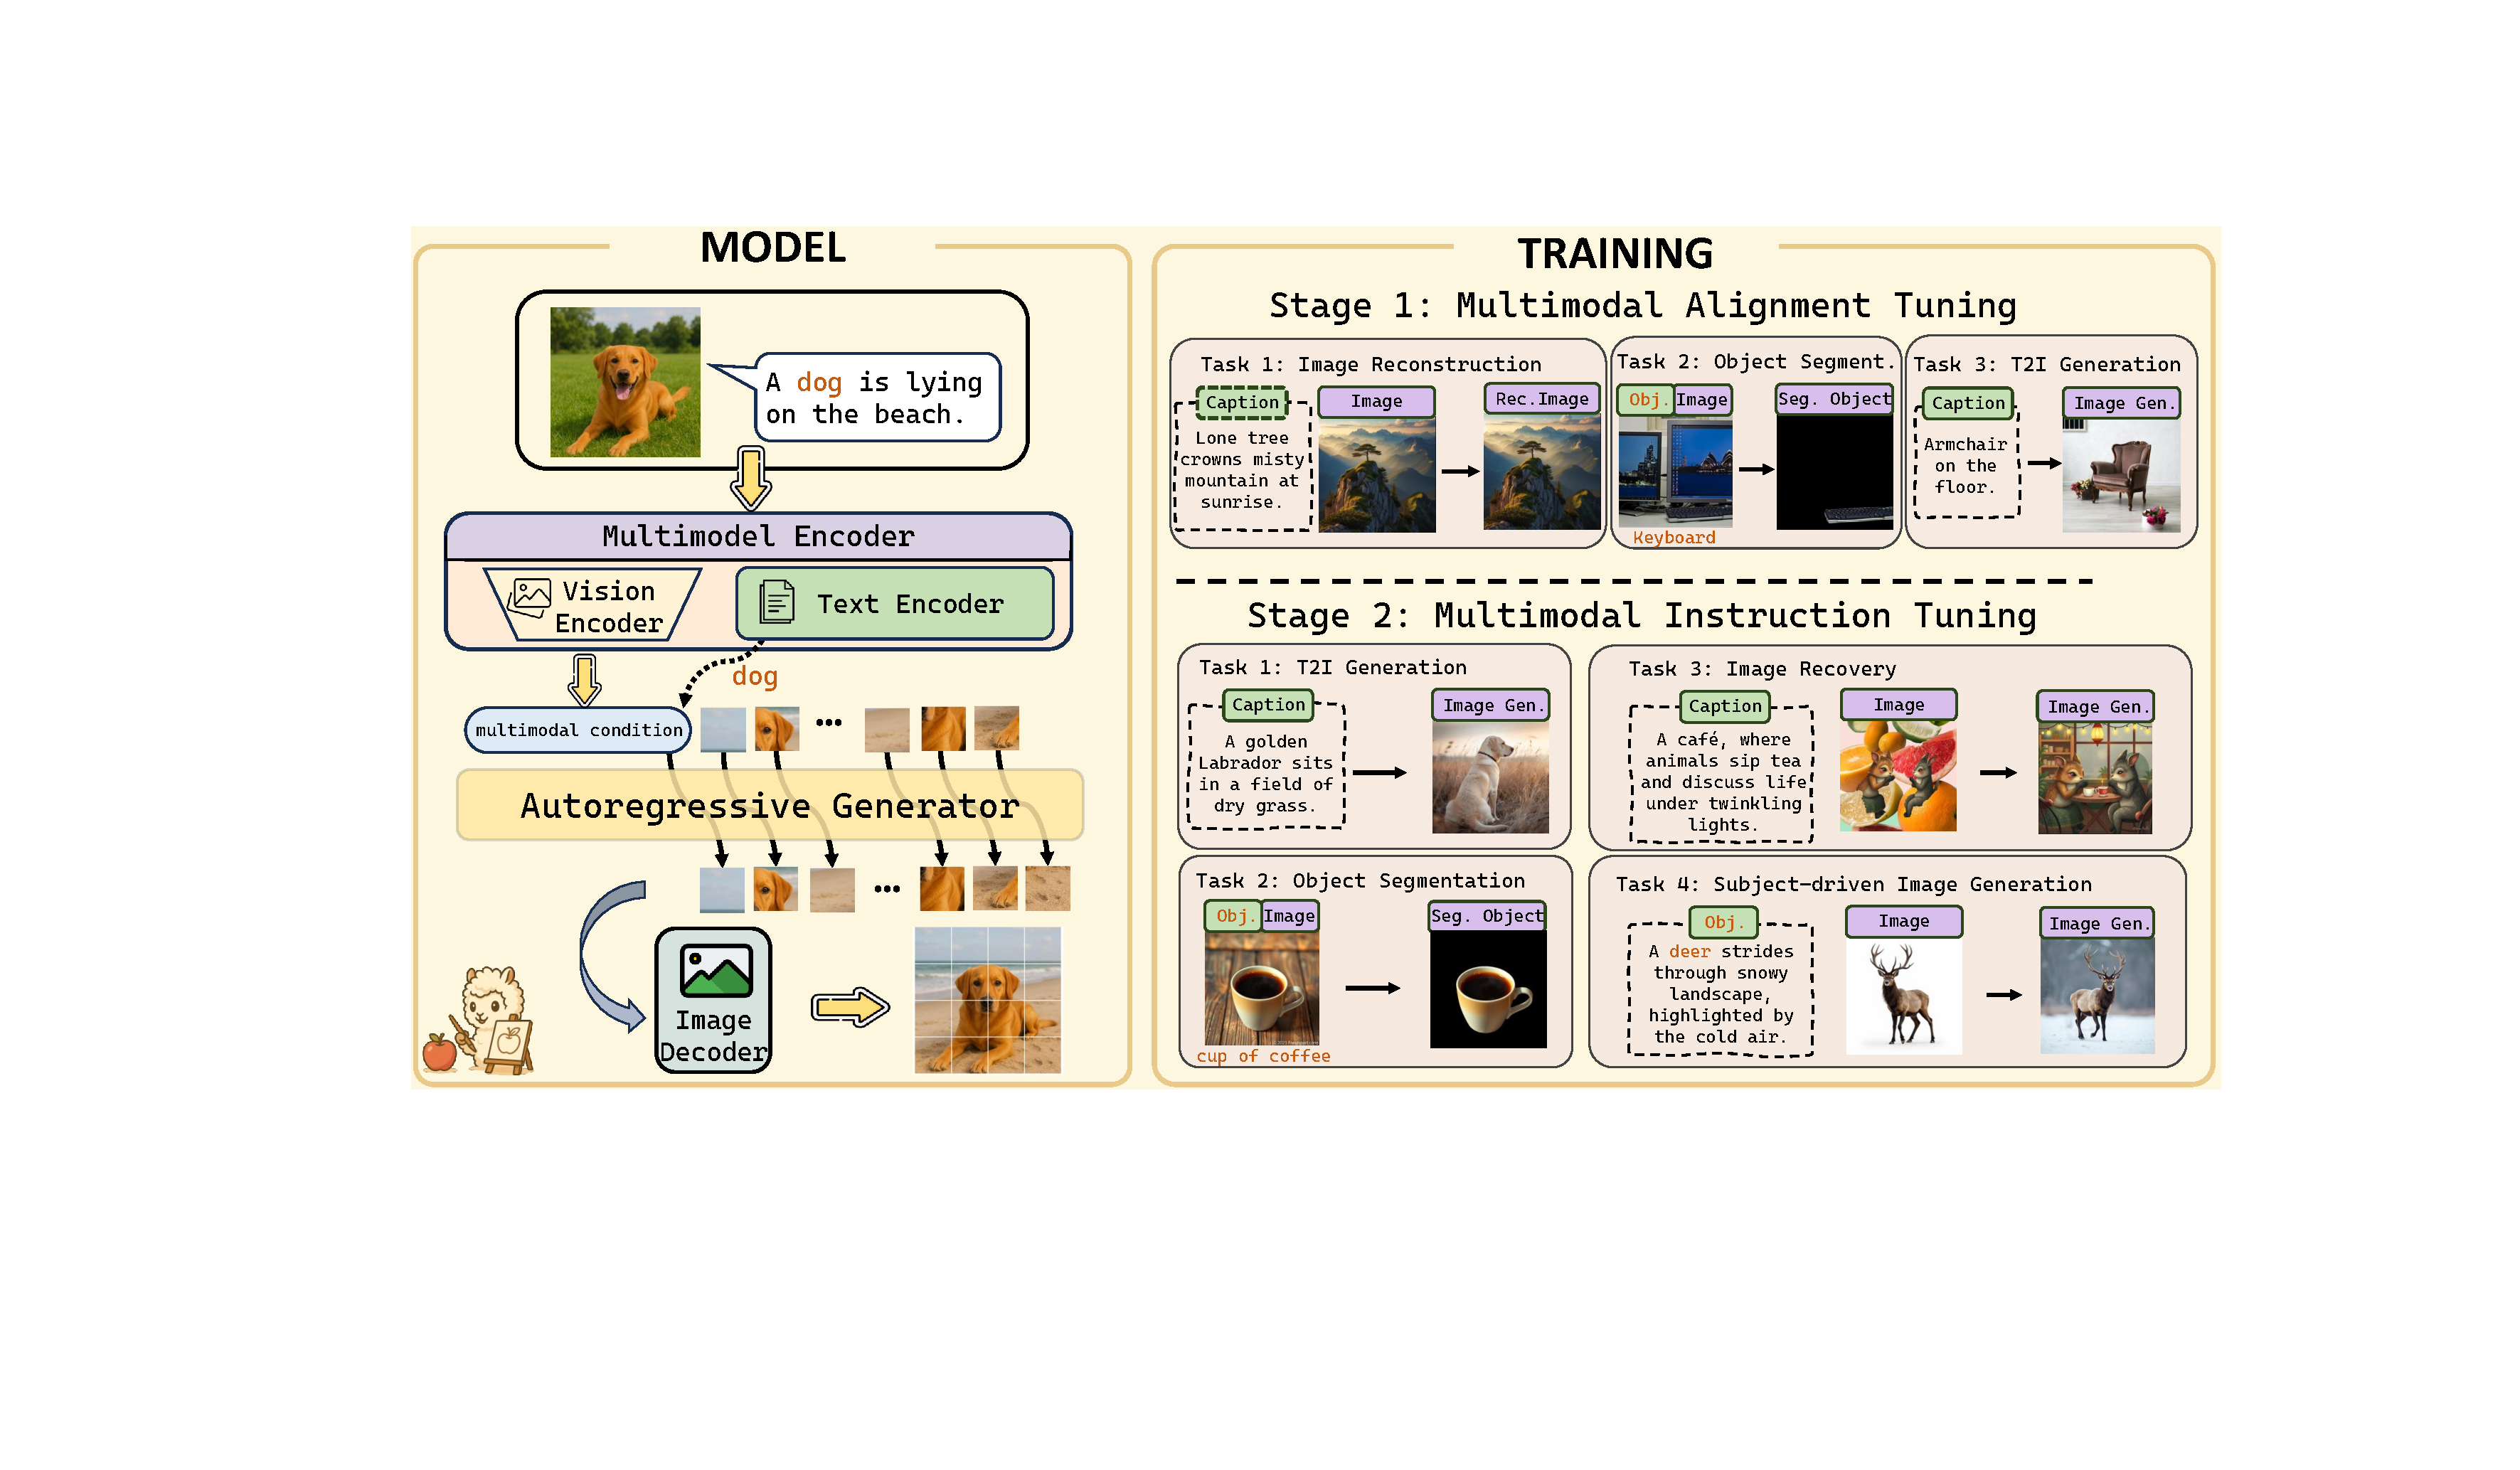
\includegraphics[width=1.0\textwidth]{figures/model_stagev2.pdf}
\caption{Overview of \model. \textbf{Left} panel illustrates the model structure, where visual and textual inputs are encoded into a unified latent to guide autoregressive image generation. \textbf{Right} panel highlights the two-stage training paradigm: (1) \textbf{Multimodal Alignment Tuning}, enabling pixel and semantic-level alignment between inputs and output tokens; and (2) \textbf{Multimodal Instruction Tuning}, compels model to effectively balance influence of different modalities.}
\label{fig:structure}
\vspace{-3ex}
\end{figure*}
\textbf{Autoregressive Generation Decoder}
A transformer-based autoregressive decoder generates a image token sequence $\mathbf{y} = (y_1, \dots, y_{L})$ conditioned on the prefix $\mathbf{H}$ generated by the multimodal encoder and previously generated tokens $y_{<i}$. It operates in a shared embedding space with the encoder's output and shares the same vocabulary as the VQGAN~\citep{Esser2020TamingTF} that is used for image tokenization.
The generated token sequences are subsequently decoded into images using the VQGAN decoder. This unified autoregressive structure facilitates unified training via next-token prediction.

% The decoder, a transformer-based autoregressive model, generates a sequence of image tokens $\mathbf{y} = (y_1, \dots, y_{L})$ conditioned on the prefix $\mathbf{h}$ and previously generated tokens $y_{<i}$. It operates in a shared embedding space with the encoder's output and uses the same discrete token vocabulary as the VQGAN employed for target image tokenization and final image synthesis from $\mathbf{y}$. This structure supports unified training via next-token prediction.

\subsection{Two-Stage Training Paradigm}
\label{sec:traing_stages}
As highlighted in the introduction, effectively aligning disparate modalities and balancing their influence are crucial challenges for multimodal conditional generation. Our carefully designed two-stage training paradigm directly addresses these issues, moving beyond initial coarse alignment to foster robust understanding and balanced integration of diverse inputs, as illustrated in \Cref{fig:structure}. 

\textbf{Stage 1: Multimodal Alignment Tuning}
While the initial connector training provides preliminary semantic alignment, we observed that the model primarily interprets visual inputs semantically like text captions, neglecting crucial visual and spatial details necessary for precise image generation. This stage is dedicated to explicitly enhancing both pixel and semantic-level modality alignment and promoting the utilization of visual information.
In Stage 1, we employ three complementary tasks:
\begin{itemize}[left=2pt, itemsep=0.5pt,topsep=0.5pt]
    \item \emph{\textbf{Image reconstruction}}, where models must faithfully reconstruct an input image conditioned on itself, with the corresponding caption randomly provided or omitted, reinforcing pixel-level fidelity.
    \item \emph{\textbf{Object segmentation}}, where models are given an input image and a target object label and must generate an end‐to‐end segmented figure for that object. This task compels the model to explicitly capture fine-grained visual details and spatial structures associated with specific semantic concepts.
    \item \emph{\textbf{T2I generation}}, using image-caption pairs to preserve and reinforce foundational generative capabilities learned during pretraining of the decoder.
\end{itemize}
Importantly, incorporating the segmentation task alongside image reconstruction mitigates the risk of the model degenerating into a trivial copy-paste behavior, such as simply replicating the input. The segmentation objective compels the model to produce semantically meaningful and spatially precise visual outputs. This complementary effect has been further analyzed and validated in \Cref{abl:stage1}.

% In Stage 1, we employ two complementary pretraining tasks:  

% \begin{itemize}[left=2pt]
% \item \emph{\textbf{image reconstruction}}, where the model must faithfully reconstruct the input image conditioned on itself, reinforcing pixel-level fidelity.
% \item \emph{\textbf{Object segmentation}}: Given an image and a target label, the model outputs an end‑to‑end segmentation of that target, cultivating fine spatial understanding and visual attention essential for visual grounding and controllable image generation.
% \item \emph{\textbf{Text-to-image generation}}: Training with image–caption pairs preserves and refines the model’s capacity to turn textual descriptions into coherent images, ensuring outputs remain firmly grounded in the input text.
% \end{itemize}

% Importantly, employing the segmentation task alongside reconstruction helps prevent from solutions—such as merely copying inputs—by requiring the model to generate semantically meaningful and spatially precise visual outputs based on multimodal conditions.

% While the preliminary alignment phase achieves coarse semantic alignment for the model, we observe that the decoder tends to treat visual inputs as text‐like captions, which predominantly captures semantic-level information, neglecting crucial pixel-level visual details necessary for precise image generation. To address this, we introduce a dedicated first stage of training designed explicitly to enhance both semantic-level and pixel-level modality alignment.

% 需要的宏包
% \usepackage{booktabs}
% \usepackage{siunitx}      % 千位分隔可选
% \sisetup{group-separator = {,}}

% %-------------------------------------------
% \begin{table}[t]
% \small
%   \begin{flushright}              % 靠右
%   \begin{minipage}{0.48\textwidth}% 右半页(≈0.5\textwidth)
%     \centering
%     \caption{Pipeline statistics}
%     \resizebox{\textwidth}{!}{%
%     \begin{tabular}{@{}l S@{}}
%       \toprule
%       \textbf{Category}       & \textbf{Value} \\
%       \midrule
%       Total                   & 3\,058\,356 \\[2pt]

%       \textbf{Stage 1}        & \textbf{2\,494\,674} \\
%       \quad t2i               & 7\,000\,000 \\
%       \quad segment           & 1\,614\,674 \\
%       \quad recover           &   180\,000 \\[2pt]

%       \textbf{Stage 2}        & \textbf{1\,313\,682} \\
%       \quad t2i               &   600\,000 \\
%       \quad segment           &   150\,000 \\
%       \quad recover           &   150\,000 \\
%       \quad subject-driven    &   413\,682 \\
%       \bottomrule
%     \end{tabular}}
%   \end{minipage}
%   \end{flushright}
% \end{table}
%-------------------------------------------


% \begin{figure*}[htbp]
%     \centering
%     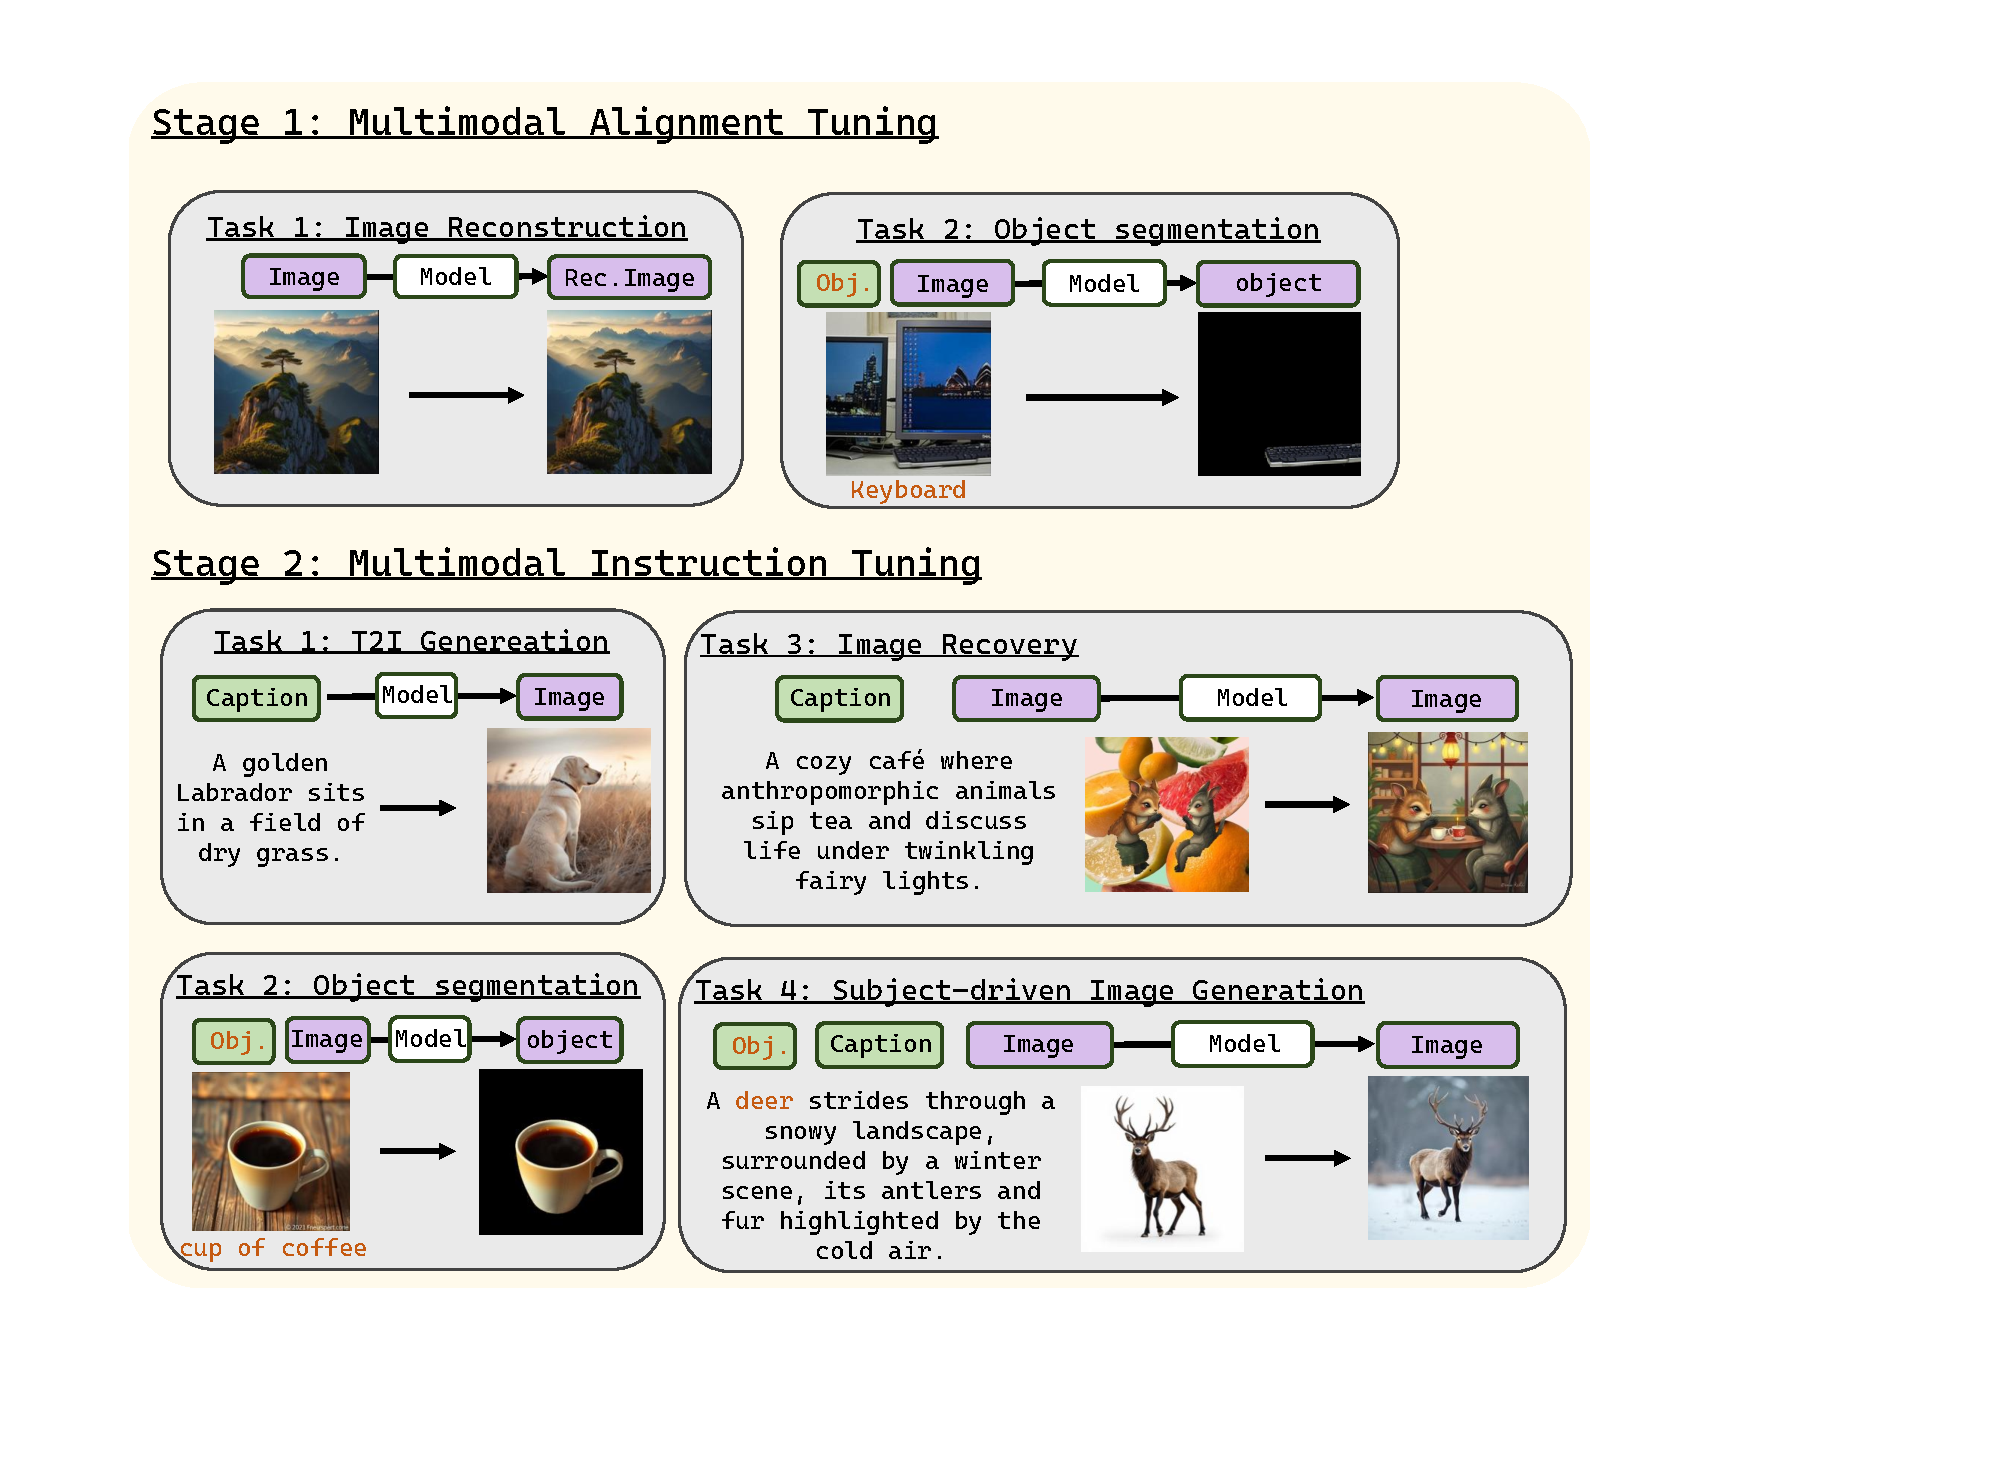
\includegraphics[width=1.0\textwidth]{figures/stages.pdf} 
%     \caption{Training Stage Placeholder
%     }
%     \label{fig:structure}
% \end{figure*}





% \begin{itemize}[left=2pt]
%     \item \emph{\textbf{Image reconstruction}}, where the model must faithfully reconstruct the input image conditioned on itself, reinforcing pixel-level fidelity.
%     \item \emph{\textbf{Object segmentation}}, where the model is given an input image and a target object label and must generate an end‐to‐end segmented figure for that object. This task compels the model to explicitly capture fine-grained visual details and spatial structures associated with specific semantic concepts.
%     \item \emph{\textbf{Text-to-image generation}}, using image-caption pairs to preserve and reinforce foundational generative capabilities learned during pretraining of the decoder.
% \end{itemize}
% Importantly, employing the segmentation task alongside reconstruction helps prevent trivial solutions—such as merely copying inputs—by requiring the model to generate semantically meaningful and spatially precise visual outputs based on the provided conditions.
% e visual outputs based on the provided conditions.


% \item \emph{\textbf{text-to-image generation}} training using image-caption pairs to preserve and reinforce foundational generative capabilities learned during pretraining of the decoder.
% \item \emph{\textbf{object segmentation}}, where the model is given an input image and a target object label and must generate an end‐to‐end segmented figure for that object. It further compels the model to explicitly capture fine-grained visual details and spatial structures associated with specific semantic concepts.
% (i)  \emph{image reconstruction}, where the model must faithfully reconstruct the input image conditioned on itself, reinforcing pixel-level fidelity; and (ii) \emph{object segmentation}, where the model is given an input image and a target object label and must generate an end‐to‐end segmented figure for that object. It further compels the model to explicitly capture fine-grained visual details and spatial structures associated with specific semantic concepts.
% Additionally, we integrate standard text-to-image generation training using image-caption pairs to preserve and reinforce foundational generative capabilities learned during pretraining of the decoder.
% Importantly, employing the segmentation task alongside reconstruction helps prevent from solutions—such as merely copying inputs—by requiring the model to generate semantically meaningful and spatially precise visual outputs based on multimodal conditions.

% Importantly, employing the segmentation task alongside reconstruction helps prevents shortcut solutions—such as directly copying inputs—by compelling the model to focus on semantically meaningful yet spatially precise visual information. Additionally, we integrate standard text-to-image generation training using image-caption pairs to preserve and reinforce foundational generative capabilities.







% The second stage of training is designed to address a central challenge in multimodal generation: ensuring the model can jointly attend to and integrate diverse input modalities in a balanced and controllable manner. 
% While the first stage focuses on aligning modalities and reinforcing the visual fidelity, Stage 2 aims to endow the model with the instruction-following ability and cross-modal reasoning capacity necessary for robust and nuanced image generation.
% Beside object segmentation and text-to-image generation, we use two additional tasks.
% To this end we adopt the multimodal instruction tuning with carefully–chosen training task. Training samples are drawn from a mixture of four complementary tasks, each targeting a distinct aspect of multimodal image generation:
% This is achieved through instruction tuning with diverse tasks designed to encourage comprehensive multimodal proficiency:

% The second stage targets enhancing the model’s capacity to jointly leverage multimodal conditions effectively during image generation, emphasizing balanced integration across modalities. 
% Specifically, we design this stage around four core training tasks to ensure comprehensive multimodal proficiency:
% \begin{itemize}[left=2pt]
% \item \emph{\textbf{Image recovery}}: Synthetically augmenting data by rotating, resizing, and compositing segmented object masks onto random backgrounds paired with original captions. This process requires the model to reconstruct the full original image, compelling it to effectively extract and integrate essential visual details from distorted contexts while relying on textual instructions to infer and restore missing components. It compels the model to fuse noisy or incomplete visual cues with textual guidance, promoting robust multimodal inference and error correction.
% \item \emph{\textbf{Subject-driven image generation}}: Conditioning on both reference images and textual instructions to serve as a final end-to-end task, fully exercising cross-modal fusion.
% \end{itemize}

% This balanced, multi-task instruction tuning ensures that the model learns to implicitly attend to and integrate both visual and textual signals harmoniously, preventing over-reliance on any single modality and yielding precise, controllable multimodal conditional generation.

\textbf{Stage 2: Multimodal Instruction Tuning}
Stage 2 aims to endow the model with robust instruction-following and cross-modal reasoning capabilities for nuanced and controllable multimodal generation, building upon the alignment and visual fidelity established in Stage 1. The model is expected to jointly attend to and integrate diverse input modalities in a balanced and controllable manner.
To achieve this, we employ a multimodal instruction tuning strategy based on a carefully curated mixture of training tasks. Specifically, we reuse the \emph{\textbf{T2I generation}} and \emph{\textbf{object segmentation}} tasks from Stage 1, maintaining identical data and formulations. These tasks respectively reinforce the model’s ability to adhere to and utilize textual and visual modalities, helping preserve foundational skills and stabilize the training process.
In addition, we introduce two novel tasks specifically designed to enhance instruction adherence and foster a balanced integration of multimodal inputs, preventing the model from over-emphasizing a single modality while neglecting others:
\begin{itemize}[left=2pt, itemsep=0.5pt,topsep=0.5pt]
    \item \emph{\textbf{Image recovery}}, where we synthetically distort images by rotating, resizing, and compositing segmented objects onto random backgrounds, then pair synthetic images with their original captions to create inputs. The model is then required to reconstruct the original image from the distorted input and corresponding caption. 
    It compels the model to extract and integrate essential visual details from noisy or incomplete visual inputs while leveraging textual cues to infer and restore missing components, promoting robust multimodal reasoning and error-correction performance.
    \item \emph{\textbf{Subject-driven image generation}}, where the model is conditioned on reference image, subject label and textual instruction to generate images. 
    It require the model to actively preserve the subject’s visual identity from the reference image while strictly adhering to the textual instructions for image generation. This task serves as a comprehensive end-to-end objective, fully exercising model’s cross-modal fusion and instruction-following abilities.
\end{itemize}
Overall, this training strategy—combining continued refinement of core capabilities with targeted instruction-based tasks—ensures the model to learn to integrate visual and textual information in a harmonious and controllable way. It mitigates over-reliance on certain modality and enables precise, controllable multimodal conditional generation, which are further discussed in \Cref{abl:stage2}. 

% \begin{figure*}[htbp]
%     \centering
%     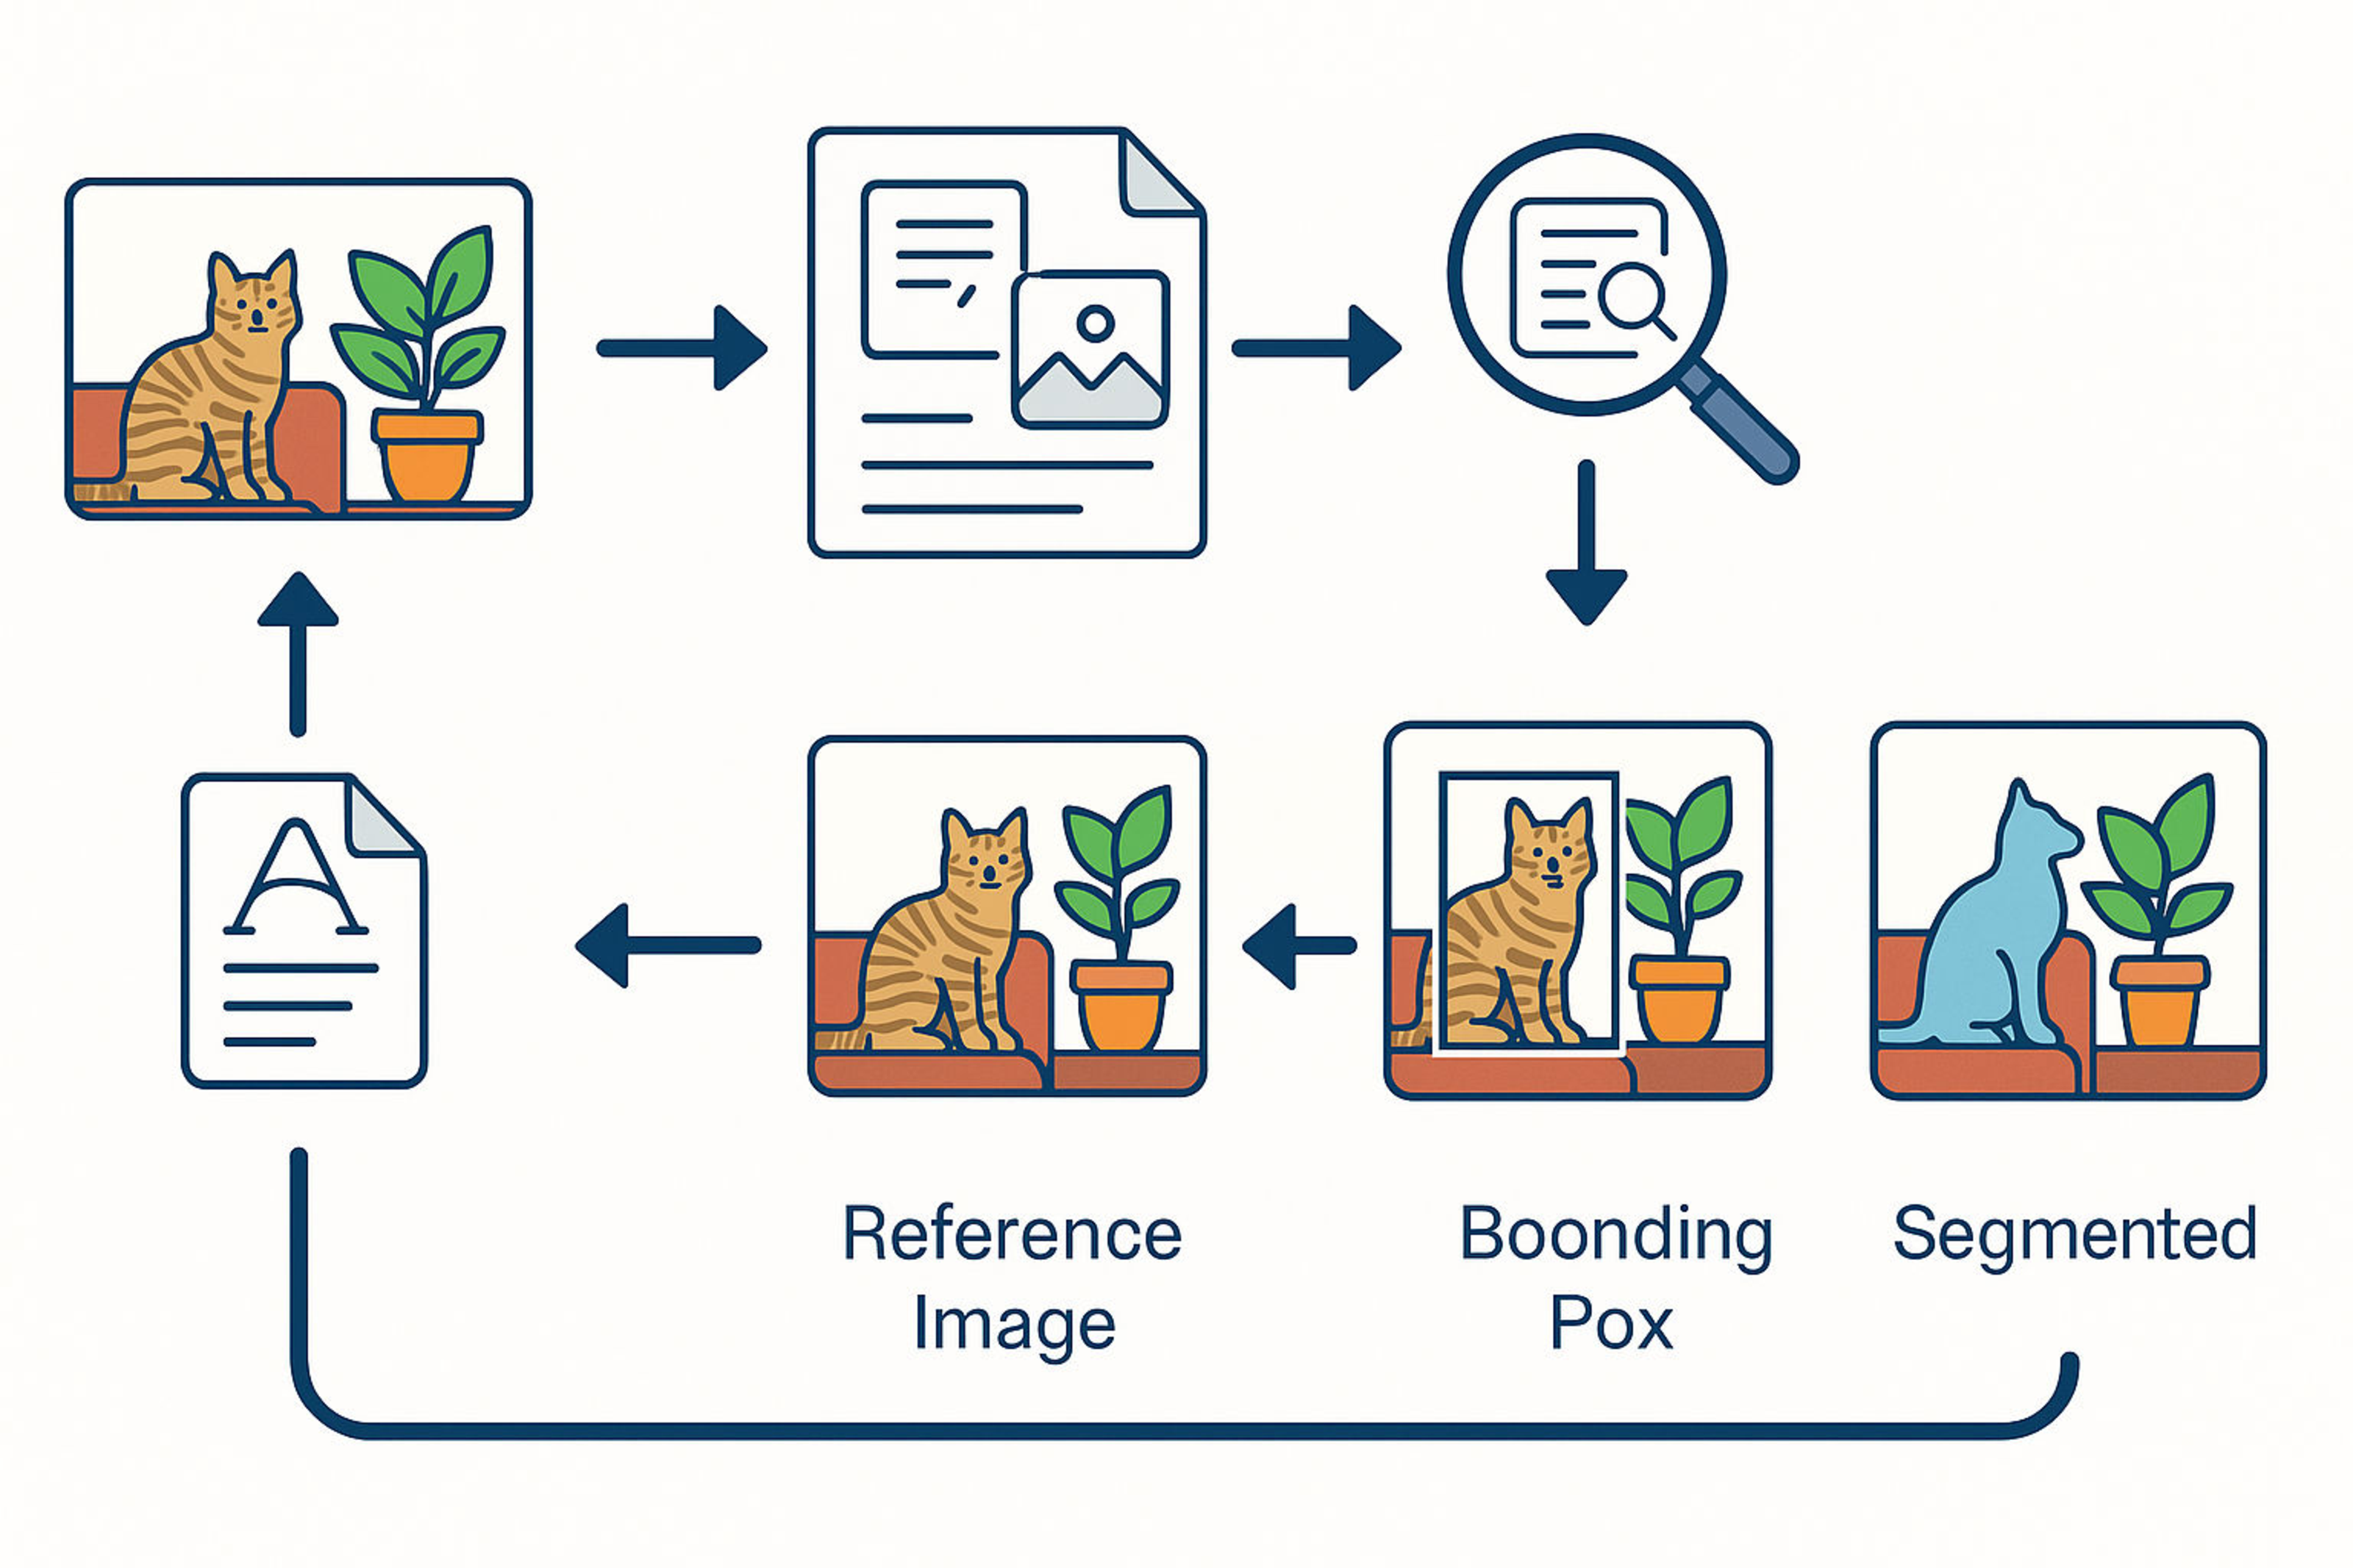
\includegraphics[width=0.8\textwidth]{figures/segment.pdf} 
%     \caption{Data construction pipeline Placeholder
%     }
%     \label{fig:structure}
% \end{figure*}


\subsection{Data Construction}
\label{sec:data_construct}

To support our two-stage training paradigm, we construct a large-scale multimodal dataset comprising approximately \textbf{3 million samples} across all training tasks. It integrates open-source resources, synthetic data, and automated annotations to ensure scalability, diversity, and strong task alignment.
For \textbf{image reconstruction} and \textbf{T2I generation}, we collect image-text pairs from datasets like CC12M~\citep{changpinyo2021cc12m} and Midjourney-Niji~\citep{midjourney-niji-1m-llavanext}.  To broaden domain coverage (e.g., human subjects, artistic scenes), we generate additional samples using T2I models like Flux.1~\citep{flux} and Stable Diffusion v3.5~\citep{2024SD3}, with prompts generated by advanced LLMs~\citep{gpt4o} to enhance semantic and visual diversity.
For \textbf{segmentation} and \textbf{image recovery}, which require fine-grained object-level annotations, we design an automated pipeline that combines state-of-the-art LMMs~\citep{Qwen2vl} with segmentation models\citep{sam}. Given an image, LMMs are queried to produce a comprehensive caption and extract a list of concrete, segmentable objects. For each object, LMMs predicts its spatial location, providing a bounding box and a set of 2D keypoints, which guide the segmentation model in producing high-quality, semantically consistent masks.
For \textbf{subject-driven image generation}, we leverage the OminiControl dataset~\citep{OminiControl}, re-captioned using LMMs to accurately extract subject-relevant descriptions. Additionally, we reverse image pairs to effectively double the usable data.
% The resulting dataset supports a wide range of multimodal tasks, including image reconstruction, T2I generation, object segmentation, and image recovery.
Data construction and formation are detailed in \Cref{sec:data_const}.




% To enable large-scale training, we design an automated pipeline that generates high-quality multimodal training data by combining open-source image datasets with the state-of-the-art vision–language models (VLMs) and segmentation models. This pipeline allows us to construct richly annotated image–text pairs containing multiple segmented foreground objects, without requiring manual labeling.

% The pipeline begins by querying a VLM to generate detailed captions and extract concrete object categories based on the image and generated caption. For each input image, we prompt the model to (1) generate a comprehensive caption that describes all visible, prominent, and foreground elements, and (2) extract a list of distinct, segmentable object names that are tangible and visually present in the image. This step ensures that only concrete and semantically meaningful visual elements are retained for downstream segmentation.

% Given the extracted object list, we then prompt the VLM again—once per object—to identify its spatial location within the image. Specifically, the model is asked to return both a tight bounding box and several representative 2D keypoints for each object. These spatial cues serve two critical roles: they constrain the region of interest for segmentation, and they reduce the likelihood of including irrelevant or overlapping background content. 

% Finally, we employ a high-performance segmentation model to extract object masks from the image, using the generated bounding boxes and keypoints. It eventually produces high-quality masks that are both semantically aligned and spatially accurate.

% By applying this pipeline to a large corpus of open-source images, we construct a multimodal dataset comprising captioned images annotated with multiple precisely segmented objects, which forms a key component of our training setup.



\section{Experiments}
\label{sec:experiments}

\subsection{Experimental Setup}
\label{sec:details}

% \textbf{Dataset Formation} 
% Approximately 3 million samples are used: Stage 1 comprises around 2.5 million, and Stage 2 has 1.3 million, with 800K overlapping. Data comes from a mix of open-source datasets like Midjourney~\citep{midjourney-niji-1m-llavanext} and CC12M~\citep{changpinyo2021cc12m}, and synthetic data created with publicly available T2I models, including Flux.1 dev~\citep{flux} and Stable Diffusion v3.5 Large~\citep{2024SD3}. More details are in \Cref{app:data_form} and \Cref{tab:dataset}.


\textbf{Implementation Details} 
The multimodal encoder is initialized using CLIP-Large-Patch14~\citep{Radford2021LearningTV} and Flant5-XL~\citep{flant5}, with a 224×224 image receptive field. 
The generator is initialized from LlamaGen-XL~\citep{llamagen}(775M). A two-layer MLP serves as the projector.
We freeze the encoder, training only the projector and generator for one epoch in Stage 1, then fine-tune the full model (except the vision encoder) for two more epochs in Stage 2.
Training on 8 A100 GPUs (80 GB each) takes about 1.5 days. More details are in \Cref{sec:Exp_Details}.
% To implement the MLP-based Projection, we train the MLP Projector on LLaVA-CC3M-Pretrain-595K data~\citep{liu2023llava}, keeping the vision and text encode frozen following the setting of LLAVA alignment training. For the Query-based Token Distillation, the model is initialized with BLIP2-Flant5-XL~\citep{li2023blip2}.

% \paragraph{Training Details}
% \label{sec:setup}


% To further investigate the effect of multi-image conditioning in multimodal generation, we continue training the model using a mixture of Stage 2 data and additional multi-subject samples generated via our data construction pipeline. In this setting, the model is tasked with reconstructing the original image based on segmented object crops and the corresponding image caption. Training is conducted for one additional epoch with a learning rate of 5e-5. Due to context length constraints, we limit each example to a maximum of three sub-images, resulting in a total sequence length of 888 tokens.

% \subsection{Evaluation Setup}


\textbf{Benchmark \& Metric.} We evaluate \model on \textbf{DreamBench}~\citep{ruiz2023dreamboothfinetuningtexttoimage} and \textbf{DreamBench\texttt{++}}~\citep{peng2025dreambenchpp} benchmarks.
\textbf{DreamBench} employs CLIP and DINO scores to measure the fidelity to images and prompts.
\textbf{DreamBench\texttt{++}} offers a scaled and diverse evaluation dataset and introduces a human-aligned automatic evaluation protocol using GPT-4o, addressing limitations of DreamBench evaluation.
GPT-4o evaluator scores generations on two axes: \textbf{Concept Preservation (CP)}, measuring the retention of the subject's visual identity, and \textbf{Prompt Following (PF)}, evaluating how accurately the image reflects the text prompt.
% Performance on DreamBench\texttt{++} is summarized by the combined CP$\cdotp$PF score, reflecting a balanced overall generation capability.
Details can be found in the \Cref{app:DreamBench_Plus}.

% \textbf{DreamBench} includes 30 subjects and 25 prompts, evaluating subject-driven generation via image–image and image–text similarity. It uses CLIP and DINO embeddings to compute subject fidelity (between the generated and reference image) and prompt fidelity (between the generated image and the prompt).

% \textbf{DreamBench\texttt{++}} significantly scales up the evaluation with 150 subjects and 1,350 prompts spanning photorealistic, stylistic, and imaginative settings. It uses GPT-4o as an automatic evaluator, scoring each image on two axes:

% \begin{itemize}
%     \item \textbf{Concept Preservation (CP):} Measures how well the generated image retains the visual identity of the reference subject (e.g., shape, color, texture, and facial details).
%     \item \textbf{Prompt Following (PF):} Evaluates how accurately the image reflects the semantics and context of the text prompt, including relevance, accuracy, and completeness.
% \end{itemize}


\textbf{Baselines.}
We compare our method against various baselines, categorized as follows:
\begin{itemize}[left=2pt, itemsep=0.5pt,topsep=0.5pt]
    \item \textbf{Fine-tuning-based methods:} Textual Inversion~\citep{gal2022imageworthwordpersonalizing}, and DreamBooth~\citep{peng2025dreambenchpp}, which fine-tune models with auxiliary control mechanisms on a subset of benchmark data.
    \item \textbf{Test Time Tuning-Free Methods:} Models pretrained on large-scale data and evaluated in a zero-shot. Diffusion-based models like BLIP-Diffusion~\citep{li2023blipdiffusionpretrainedsubjectrepresentation}, Emu2~\citep{emu2}, variants of IP-Adapter~\citep{ye2023ip-adapter}, and DreamEngine~\citep{dreamengine}, as well as autoregressive models like Unified-IO 2~\citep{lu2023unifiedio2} and Lumina-mGPT~\citep{2024lumina}. 
\end{itemize}

% \textbf{Baselines.} We compare our method against a range of baselines, categorized as follows:

% \noindent\makebox[2pt][l]{•}~\textbf{Fine-tuning-based methods.} Textual Inversion~\citep{gal2022imageworthwordpersonalizing} and DreamBooth~\citep{peng2025dreambenchpp}, which fine-tune models with auxiliary control mechanisms on subsets of benchmark data.

% \noindent\makebox[2pt][l]{•}~\textbf{Test-time tuning-free methods.} These models are pretrained on large-scale multimodal data and evaluated in a zero-shot setting without subject-specific fine-tuning. This category includes diffusion-based models such as BLIP-Diffusion~\citep{li2023blipdiffusionpretrainedsubjectrepresentation}, Emu2~\citep{emu2}, variants of IP-Adapter~\citep{ye2023ip-adapter}, and DreamEngine~\citep{dreamengine}, as well as autoregressive models like Unified-IO 2~\citep{lu2023unifiedio2} and Lumina-mGPT~\citep{2024lumina}.



\subsection{Main results}
\label{sec:main}
\Cref{tab:comparison} comprehensively evaluates our proposed autoregressive (AR) framework on the DreamBench++ benchmark, comparing it with diffusion-based and autoregressive-based baselines.
\model demonstrates highly competitive performance, particularly in achieving a strong balance between the guidance of both input modalities. Notably, this is achieved despite utilizing significantly fewer training resources and suboptimal model components compared to the state-of-the-art baselines.
% We assess performance along two key axes: Concept Preservation (CP)—measuring fidelity to the reference subject—and Prompt Following (PF)—evaluating semantic alignment with the textual prompt.

\textbf{Overall Performance.}
\model achieves a strong balance between concept fidelity and prompt alignment, resulting in the high \textbf{CP$\cdotp$PF} score. 
% Notably, even without task-specific fine-tuning and using a modest model size and training data, 
\model rivals fine-tuned methods like DreamBooth-LoRA, while significantly outperforming test-time tuning-free baselines such as Emu2 and DreamEngine. For instance, \model surpasses Emu2 in CP$\cdotp$PF score by approximately 30\%. 
% While fine-tuning methods like DreamBooth LoRA (0.52) achieve a higher CP$\cdotp$PF score, they benefit from training directly on the test set subjects, whereas our method operates in a test-time tuning-free manner.
A key strength of \model is its ability to harmoniously integrate multimodal inputs. Several strong baselines, including some AR methods like Lumina-mGPT and Unified-IO2, exhibit very high Concept Preservation (CP) but suffer from extremely low Prompt Following (PF), resulting in high \textbf{CP/PF} scores. This indicates a tendency to over-rely on the reference image while neglecting textual instructions. In contrast, \model delivers lowest CP/PF scores compared to all test-time tuning-free baselines, demonstrating effective and controlled integration of both visual and textual guidance.


\begin{table}[t]
\vspace{-8ex}
\centering
\small
\caption{
Comparison on DreamBench++. Models are ranked by \textbf{CP$\cdotp$PF}, indicating balanced overall multimodal image generation performance. \textbf{CP/PF} ratio reflects overfitting issue toward certain modality. ``*'' denotes model trained \textbf{from scratch}; others are adapted from pre-trained T2I models.
}

\label{tab:comparison}
\resizebox{\textwidth}{!}{%
\begin{tabular}{@{}l@{\hspace{1ex}}c@{\hspace{1ex}}c@{\hspace{1ex}}c@{\hspace{1ex}}c@{\hspace{1ex}}c@{\hspace{1ex}}c@{\hspace{1ex}}c@{\hspace{1ex}}c@{\hspace{1ex}}c@{\hspace{1ex}}c@{\hspace{1ex}}c@{\hspace{1ex}}c@{\hspace{1ex}}c@{\hspace{1ex}}c@{}}
\toprule
\textbf{Method} & \textbf{T2I Model} & \textbf{Train Data} & \textbf{Model Size} 
& \multicolumn{5}{c}{\textbf{Concept Preservation (CP)}} 
& \multicolumn{4}{c}{\textbf{Prompt Following (PF)}} 
& \textbf{CP$\cdotp$PF} & \textbf{CP/PF} \\
\cmidrule(lr){5-9} \cmidrule(lr){10-13}
& & & & \textbf{Animal} & \textbf{Human} & \textbf{Object} & \textbf{Style} & \textbf{Overall} 
& \textbf{Photo.} & \textbf{Style.} & \textbf{Imag.} & \textbf{Overall} & & \\
\midrule
\multicolumn{15}{c}{\textbf{Finetuned on Test Set}} \\
\midrule
Textual Inv.         & SD v1.5      & -     & 860M    & 0.50 & 0.36 & 0.31 & 0.36 & 0.38 & 0.67 & 0.69 & 0.44 & 0.62 & 0.24 & 0.61 \\
DreamBooth           & SD v1.5      & -     & 860M    & 0.64 & 0.20 & 0.49 & 0.48 & 0.49 & 0.79 & 0.78 & 0.50 & 0.72 & 0.36 & 0.68 \\
DreamBooth-L         & SDXL v1.0    & -     & 2.60B   & 0.75 & 0.31 & 0.54 & 0.72 & 0.60 & 0.90 & 0.90 & 0.75 & 0.87 & 0.52 & 0.69 \\

\midrule
\multicolumn{15}{c}{\textbf{Test-Time Tuning-Free Methods}} \\
\midrule
Unified-IO2*         & Unified-IO2  & 8.5B    & 7.00B   & 0.77 & 0.80 & 0.64 & 0.82 & 0.72 & 0.24 & 0.18 & 0.11 & 0.19 & 0.14 & 3.79 \\
Lumina-mGPT          & Chameleon    & 10M     & 7.00B   & 0.95 & 0.97 & 0.89 & 0.85 & 0.91 & 0.31 & 0.25 & 0.15 & 0.25 & 0.23 & 3.64 \\

DreamEngine          & SD3.5        & 21M     & 10.50B  & 0.76 & 0.72 & 0.61 & 0.73 & 0.68 & 0.44 & 0.37 & 0.25 & 0.37 & 0.26 & 1.84 \\

BLIP-Diffusion       & SD v1.5      & 130M    & 1.56B   & 0.67 & 0.56 & 0.47 & 0.51 & 0.55 & 0.58 & 0.51 & 0.30 & 0.50 & 0.27 & 1.10 \\

Kosmos-G             & SD v1.5      & 200M    & 3.00B   & 0.62 & 0.63 & 0.46 & 0.57 & 0.54 & 0.48 & 0.62 & 0.41 & 0.51 & 0.28 & 1.06 \\

IP-A-Plus ViT-H      & SDXL v1.0    & 10M     & 3.00B   & 0.90 & 0.85 & 0.76 & 0.91 & 0.83 & 0.50 & 0.38 & 0.28 & 0.41 & 0.34 & 2.02 \\

Emu2                 & SDXL v1.0    & 16M     & 37.00B  & 0.67 & 0.55 & 0.45 & 0.45 & 0.53 & 0.73 & 0.72 & 0.56 & 0.69 & 0.36 & 0.77 \\

IP-A ViT-G           & SDXL v1.0    & 10M     & 2.50B   & 0.67 & 0.56 & 0.50 & 0.75 & 0.59 & 0.74 & 0.63 & 0.45 & 0.64 & 0.38 & 0.92 \\
\rowcolor{gray!20} \model & LlamaGen & 3M      & 2.31B   & 0.65 & 0.36 & 0.57 & 0.47 & 0.55 & 0.86 & 0.85 & 0.80 & 0.84 & \textbf{0.47} & \textbf{0.65} \\
\bottomrule
\end{tabular}%
}
\end{table}



% Importantly, despite relying on a relatively low-quality image generator and sub-optimal encoders, our method excels in multimodal conditioning tasks. This suggests that the improved alignment and interaction between modalities enabled by our autoregressive design outweigh the limitations in token-level reconstruction quality inherent to discrete AR generation. As further shown in \Cref{tab:fid_comparison}, our model underperforms in traditional text-to-image metrics due to reconstruction loss and limited training data and model size; however, it excels in multimodal guidance, highlighting the core strength of our framework.
\textbf{Training Efficiency.}
A notable advantage of \model lies in its training efficiency. It is trained on only 3 million image-text pairs across two stages, substantially less than leading baselines, such as Emu2 (16M), Kosmos-G (200M), and DreamEngine (21M).
Beyond the reduced data requirements, the training process is highly resource-efficient: the entire training process completes in 1.5 days with 8 GPUs. This contrasts sharply with other baselines, such as Kosmos-G, which necessitates 256 GPUs over three days.
Despite this dramatically reduced computational and data budgets, \model achieves SOTA performance with balanced performance, highlighting its efficiency and effectiveness.
Furthermore, \model remains highly competitive in size compared to larger counterparts like Emu2 (37B parameters) and DreamEngine (10.5B parameters), highlighting our framework's effectiveness.


% These findings demonstrate that exposure to diverse object views during training improves the model’s ability to generalize visual identity under limited test conditions. Moreover, unlike many diffusion models that exhibit modality dominance (e.g., overemphasizing style or text), our AR framework integrates multiple inputs without sacrificing textual adherence—highlighting its scalability in complex multimodal scenarios.

% 

\textbf{Discussion and Connection to Methodology.}
The strong performance of \model — particularly its balanced multimodal generation and training efficiency — stems from its \textbf{autoregressive nature} and \textbf{two-stage training paradigm}.
The \textbf{autoregressive design}, which generates image tokens sequentially conditioned on a unified multimodal prefix, enables fine-grained, token-level alignment between inputs and outputs. This direct alignment significantly enhances prompt following, ensuring generated images accurately reflect both text and visual guidance.
The \textbf{two-stage training paradigm} is also critical for balanced multimodal control. It mitigates the common issue of over-reliance on one modality while ignoring others, resulting in significantly improved CP$\cdotp$PF scores compared to baselines.
Notably, \model achieves strong results despite using \textbf{relatively suboptimal components}.
While other baselines rely on advanced models such as Qwen-2.5 and SD3, we use Flan-T5 as the encoder and LlamaGen as the generator — both of which greatly underperform stronger counterparts, as shown in \Cref{tab:fid_comparison} and \Cref{tab:exp-geneval}. 
This highlights that our performance gains are driven by methodological strength, not from scaling up model capacity.
While performance on out-of-distribution or fine-grained categories remains limited due to the suboptimal components, \model maintains strong overall results by effectively integrate multimodal inputs for generation.




% The strong performance of our AR framework, especially its balanced CP and PF scores and high training efficiency, can be attributed to several key aspects of our methodology.
% The autoregressive nature of our method, which generates image tokens sequentially conditioned on a unified multimodal prefix, facilitates precise, token-level integration between the conditions and generated images. This direct alignment likely contributes to the high Prompt Following scores.
% Furthermore, our proposed two-stage training paradigm is crucial for achieving balanced multimodal control. 
% The first stage aims to enhances both pixel-level and semantic-level alignment, fostering better Concept Preservation. Stage 2 explicitly trains the model to effectively leverage and balance varied multimodal inputs
% It prevents the model from overemphasizing one modality (e.g., the reference image) at the expense of others (e.g., the text prompt), a common pitfall observed in other methods, and outperforms other baselines in CP$\cdotp$PF score.

% It is particularly noteworthy that our framework achieves impressive results despite using suboptimal components compared to others. For instance, we use a Flan-T5-XL as encoder, while others use more advanced models like Vicuna and Qwen-2.5. Additionally, our autoregressive generator (LlamaGen-XL) underperforms against advanced large scale diffusion models such as SDXL or SD3.5, and even earlier models like SD1.5. 
% This highlights the strength of our proposed framework. The direct multimodal alignment from the AR framework, and the significant impact of our two-stage training strategy in optimizing multimodal conditional image generation.

% Nevertheless, we acknowledge current limitations: due to the sub-optimal quality of our multimodal encoder and AR generator, performance on out-of-distribution or fine-grained human categories remains less robust. As shown in \Cref{tab:fid_comparison}, the text-to-image quality of our generation model lags behind SOTA diffusion models. However, the ability of our model to leverage multimodal inputs more effectively enables it to compensate for these weaknesses and maintain strong overall performance.

% Our results clearly demonstrate that the proposed autoregressive framework, even with modest data and compute resources, achieves state-of-the-art multimodal generation performance. Through architectural simplicity, efficient training, and balanced attention across modalities, our method offers a scalable and controllable alternative to diffusion-based approaches, setting a new standard for autoregressive multimodal image generation.








\subsection{Ablation Study}
\label{sec:ablation}

We conduct a ablation study on DreamBench++ and DreamBench focusing on two central questions: (1) How critical is Stage 1 for robust multimodal alignment? and (2) What role does each Stage 2 training task play in shaping model’s multimodal generation behavior?
Following prior work~\citep{peng2025dreambenchpp}, we report \textbf{CP$\cdot$PF} as a primary measure of multimodal image generation ability.
% We conduct the ablation study on both DreamBench++ and DreamBench benchmarks. Following prior work, we report the harmonic mean of Concept Preservation (CP) and Prompt Following (PF)—denoted as \textbf{CP$\cdotp$PF}—as a primary measure of multimodal generation quality. For all settings, we train for two epochs with consistent hyperparameters and average results over three random seeds. The results are presented in \Cref{tab:ablation_combined}.

\textbf{Importance of Stage 1: Foundational Multimodal Alignment.} \label{abl:stage1}
As shown in \Cref{tab:ablation_combined}, removing Stage 1 leads to the most severe performance drop, underscoring its foundational role. On DreamBench++, the CP score drops from 0.555 to 0.179, indicating a major loss in visual identity preservation, with PF also significantly reduced. Similar trends appear on DreamBench.
Ablating only \textbf{object segmentation task} in Stage 1 (\textit{w/o Obj. Seg. in Stage 1}) also hampers model performance.
While the remaining image reconstruction task supports pixel-level alignment, allowing for reconstruction of input images, it inadvertently leads the model to exhibit a copy-paste behavior, failing to capture semantic and visual information of input images. It confirms that reconstruction alone is insufficient for robust multimodal alignment.
Overall, these results highlight Stage 1 as critical for aligning multimodal inputs with output images.
Without such alignment, the model struggles to ground visual concepts from images, severely impairing its visual preservation ability.


\textbf{Contributions of Different Training tasks in Stage 2.} \label{abl:stage2} 
The distinct contributions of different Stage 2 tasks are also evident in \Cref{tab:ablation_combined}.
Excluding the \textit{Image Recovery} task leads to a sharp imbalance: while visual preservation metrics (CP, DINOv1, CLIP-I) show a notable increase, instruction following ability (PF and CLIP-T score) critically drops, showing an overfitting to visual features. This underscores that image recovery acts as a critical regularizer, encouraging the model to reconstruct incomplete visual contexts guided by text prompt, thereby fostering a balanced use of different modalities.
Conversely, ablating either the \textit{Object Segmentation} or the \textit{Subject-Driven Image generation} significantly degrades visual preservation ability, as these tasks prompt the model to utilize the visual features of the input image effectively to generate images.
Without these tasks, the model tends to over-rely on textual prompts, resulting in a regression towards a standard T2I model that neglects the reference image. 
These results highlight the importance of all Stage 2 tasks: image recovery ensures cross-modal balance, while object segmentation and subject-driven generation enhance the model’s ability to extract and utilize detailed visual information for image generation.
% It highlights the importance of object segmentation and subject-driven image generation in refining the model's ability to capture fine-grained visual details
% Although the instruction following ability seems slightly enhanced, it comes at the expense of neglecting visual features, resulting in generated images that often misaligned with the intended visual appearance from the input image. 
% Thus, object segmentation and subject-driven image generation are essential for enforcing spatial awareness and enhancing pixel-level subject integrity.

% \paragraph{Summary.}
% In essence, the ablation results confirm that all examined components of our two-stage training are vital. Stage 1 provides essential multimodal grounding, while each task in Stage 2 uniquely contributes to enhancing concept fidelity, ensuring textual adherence, or promoting a harmonious balance between them. Our model's superior performance is a direct outcome of this carefully orchestrated training strategy.



\begin{table}[t]
\vspace{-8ex}
\centering
\small
\caption{Ablation results on DreamBench++ and DreamBench.
% CP$\cdotp$PF denotes the harmonic mean between Concept Preservation (CP) and Prompt Following (PF). Our full model achieves the best trade-off across both benchmarks.
}
\label{tab:ablation_combined}
\resizebox{\linewidth}{!}{%
\begin{tabular}{lcccccc}
\toprule
\multirow{2}{*}{\textbf{Method}} &
\multicolumn{3}{c}{\textbf{DreamBench++}} &
\multicolumn{3}{c}{\textbf{DreamBench}} \\
\cmidrule(lr){2-4} \cmidrule(lr){5-7}
 & \textbf{CP} & \textbf{PF} & \textbf{CP$\cdotp$PF} 
 & \textbf{DINOv1} & \textbf{CLIP-I} & \textbf{CLIP-T} \\
\midrule
\textit{w/o Obj. Seg. in Stage 1}   
& $0.252 \pm 0.004$ & $0.479 \pm 0.005$ & $0.121$ 
& $56.113 \pm 0.082$  & $74.384 \pm 0.071$  & $23.965 \pm 0.038$ \\

\textit{w/o Stage 1 Alignment}     
& $0.179 \pm 0.002$ & $0.673 \pm 0.012$ & $0.120$ 
& $33.523 \pm 0.111$  & $67.705 \pm 0.101$  & $28.263 \pm 0.155$ \\

\textit{w/o Image Recovery}        
& $0.661 \pm 0.007$ & $0.284 \pm 0.004$ & $0.188$ 
& $74.471 \pm 0.321$ & $81.280 \pm 0.094$ & $24.210 \pm 0.022$ \\

\textit{w/o Object Segmentation}   
& $0.412 \pm 0.002$ & $0.918 \pm 0.003$ & $0.378$ 
& $57.221 \pm 0.119$  & $76.269 \pm 0.084$  & $31.078 \pm 0.050$ \\

\textit{w/o Multimodal T2I Task}   
& $0.407 \pm 0.004$ & $0.910 \pm 0.004$ & $0.370$ 
& $58.880 \pm 0.143$  & $76.529 \pm 0.102$  & $30.483 \pm 0.002$ \\

\rowcolor{gray!10}
\textbf{\model}         
& $0.555 \pm 0.006$ & $0.839 \pm 0.002$ & $\mathbf{0.466}$ 
& $70.853 \pm 0.327$  & $80.911 \pm 0.053$  & $29.071 \pm 0.080$ \\
\bottomrule
\end{tabular}%
}
\end{table}

\subsection{Analysis}
\label{sec:Analysis}

\textbf{Efficiency and Effectiveness: AR vs. Diffusion.}
To evaluate the efficiency of our AR framework against diffusion-based approaches, we conducted a controlled comparison with \textbf{Kosmos-G}~\citep{Kosmos-G}, a representative LMM-augmented diffusion model.Both models were trained from similar initializations on the same training data to ensure a fair comparison. Despite Kosmos-G employing a superior SD1.5 generator and Kosmos-1 as encoder, \model, which utilizes a underperformed LlamaGen generator and a FlanT5 based encoder, demonstrated significantly better performance on DreamBench++ as shown in \Cref{tab:comparison}.
It highlights the effectiveness of \model in fostering efficient multimodal learning and strong multimodal conditional generation.




\textbf{Comparison of Proposed Architecture Variants. }
As shown in \Cref{tab:ablation_combined}, we compare two architectural variants of \model: the MLP-based connector (\model) and a Query-based connector for the multimodal encoder. It reveals that an MLP-based connector significantly outperforms the query-based variant in CP scores, especially for humans and objects. It suggests that after visual token compression, the query-based approach struggles to retain fine-grained visual details, which are crucial for generative fidelity, even when guided by textual queries.
Nevertheless, due to effective token distillation, the Query-based variant facilitates training with multiple contextual images with minimal computational resources.
Despite these differences, both variants exhibit competitive performance compared to other baselines in \Cref{tab:comparison}. This demonstrates that our simple and coherent architecture can effectively propagate visual features, whether or not perform aggressive visual token compression, highlighting the flexibility and robustness of our framework.




% The MLP-based variant demonstrates superior performance, particularly in Concept Preservation. The Query-based variant suffers from a significant drop in CP, particularly for humans and objects. It suggests that after visual token compression, even when guided by textual queries, the model still loses fine-grained visual details crucial for generation fidelity.
% However, the Query-based variant, through token distillation, efficiently supports multi-image generation, enabling the training of a dozen of images for generation with the same computational resources. 
% \Cref{} illustrates examples of this multi-image generation using the Query-based variant.
% The MLP-based variant, designed to minimize information loss, effectively preserves visual details of reference images within our AR generation process.
% Despite these differences, both variants perform competitively compared to other baselines in \Cref{tab:comparison}. This confirms that our simple and coherent architecture allows for effective propagation of visual features throughout the generation process, with or without aggressive compression, enabling robust adaptation to various input formats.


% \begin{figure*}[tbhp]
% \centering
% \begin{minipage}[c]{0.42\textwidth}  % 改为 [c],垂直居中对齐
%     \centering
%     \captionof{table}{Image reconstruction performance (L2 distance) on COCO and JourneyDB datasets.}
%     \label{tab:reconstruct_l2}
%     \vspace{1ex}  % 可调整,增加表格与标题间距
%     \resizebox{\textwidth}{!}{
%     \begin{tabular}{@{}lcc@{}}
%     \toprule
%     \textbf{Method} & \textbf{COCO ($\downarrow$)} & \textbf{JourneyDB ($\downarrow$)} \\
%     \midrule
%     SeedTokenizer   & 0.5102 & 0.5291 \\
%     SEED-X          & 0.4317 & 0.4352 \\
%     EMU2-Gen        & 0.3828 & 0.2869 \\
%     DreamEngine     & \underline{0.2065} & \underline{0.2052} \\
%     \midrule
%     \textbf{Ours}   & \textbf{0.1008} & \textbf{0.0867} \\
%     \bottomrule
%     \end{tabular}
%     }
% \end{minipage}%
% \hfill
% \begin{minipage}[c]{0.56\textwidth}  % 同样改为 [c]
%     \centering
%     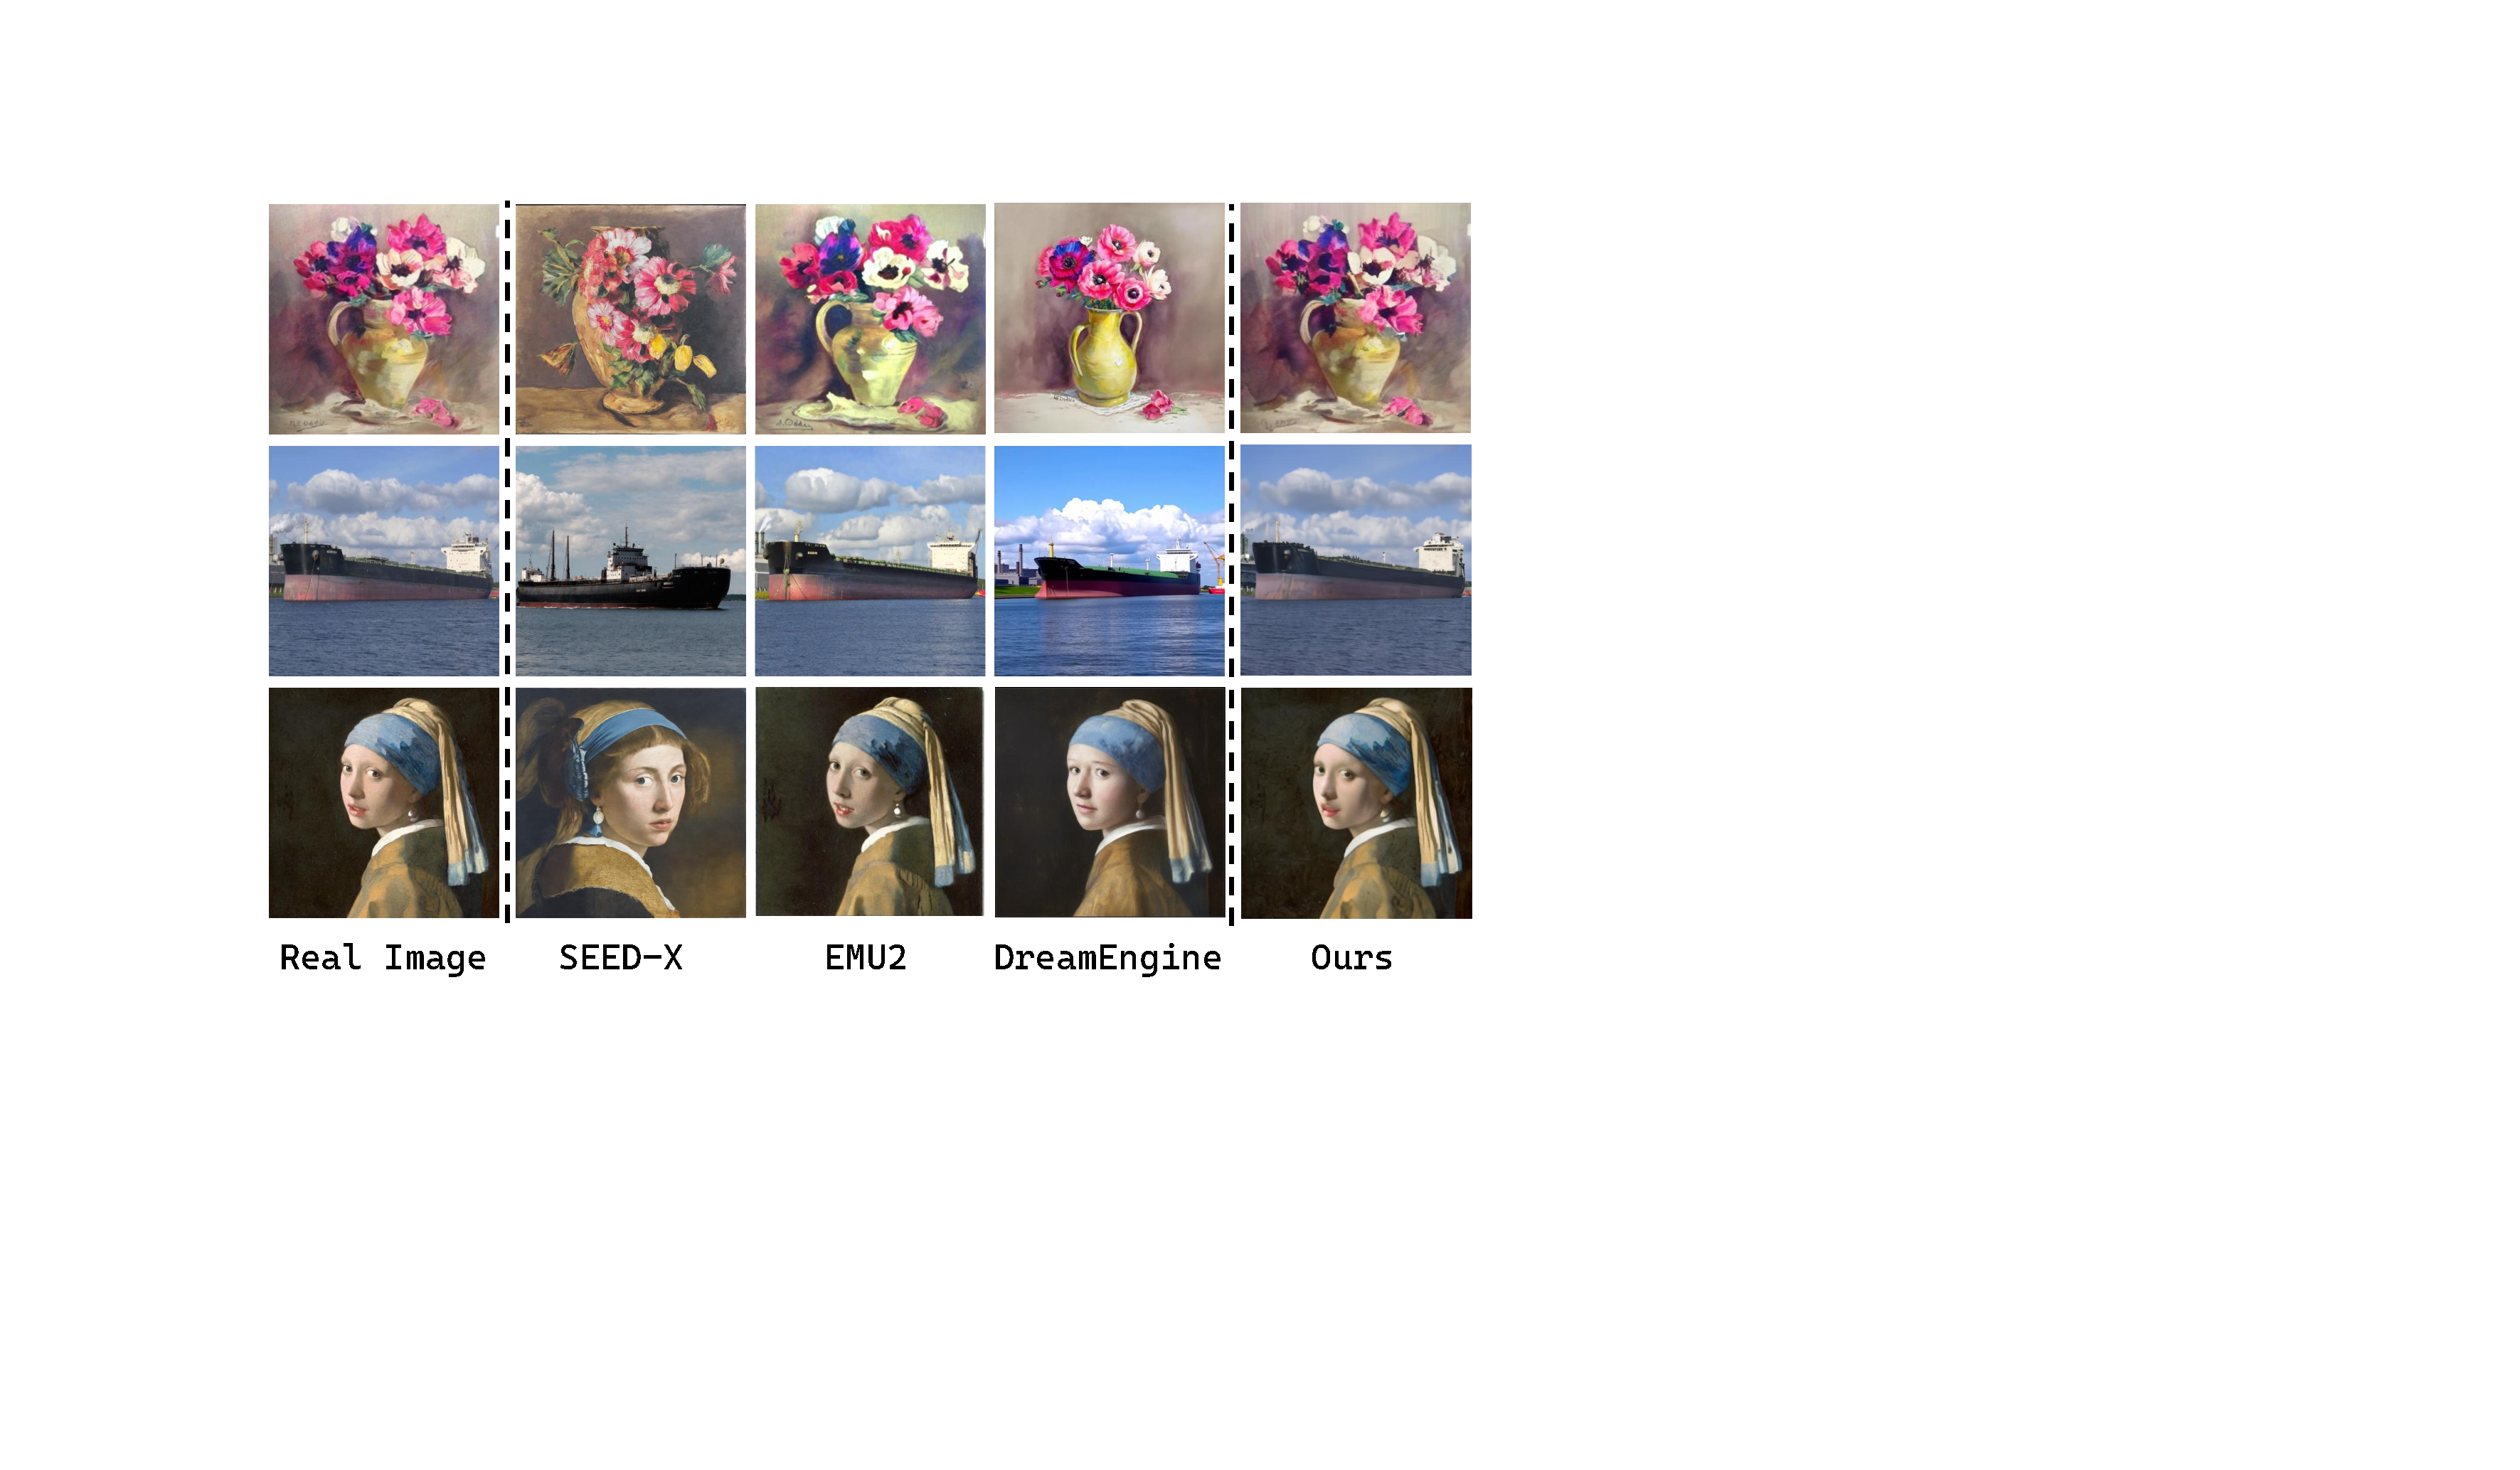
\includegraphics[width=\textwidth]{figures/reconstruction_exp.pdf}
%     \captionof{figure}{Image reconstruction results of various methods~\citep{dreamengine,2024SeedX,emu2}.}
%     \label{fig:reconstruction}
% \end{minipage}
% \end{figure*}



\begin{table}[t]
\vspace{-8ex}
\centering
\caption{Controllable experiments between \model and Kosmos-G in DreamBench++ benchmark.}
\label{tab:comparison}
\resizebox{\textwidth}{!}{%
\begin{tabular}{@{}lcccccccccc@{}}
\toprule
\textbf{Method} & \multicolumn{5}{c}{\textbf{Concept Preservation (CP)}} & \multicolumn{4}{c}{\textbf{Prompt Following (PF)}} & \textbf{CP$\cdotp$PF} \\ 
\cmidrule(lr){2-6} \cmidrule(lr){7-10}
 & \textbf{Animal} & \textbf{Human} & \textbf{Object} & \textbf{Style} & \textbf{Overall} & \textbf{Photorealistic} & \textbf{Style Transfer} & \textbf{Imaginative} & \textbf{Overall} & \\ 
\midrule
Kosmos-G  & 0.17 & 0.08 & 0.14 & 0.18 & 0.15 & 0.72 & 0.71 & 0.68 & 0.71 & 0.11 \\
\model     & 0.65 & 0.36 & 0.57 & 0.47 & \textbf{0.55} & 0.86 & 0.85 & 0.80 &\textbf{0.84} & \textbf{0.47} \\ 
\bottomrule
\end{tabular}%
}
\vspace{-2ex}
\end{table}


\begin{table}[t]
\centering
\vspace{-2ex}
\small
\caption{Ablation studies on architecture design and multi-image training}
\label{tab:ablation_combined}
\resizebox{\linewidth}{!}{%
\begin{tabular}{lcccccc}
\toprule
\multirow{2}{*}{\textbf{Method}} &
\multicolumn{3}{c}{\textbf{DreamBench++}} &
\multicolumn{3}{c}{\textbf{DreamBench}} \\
\cmidrule(lr){2-4} \cmidrule(lr){5-7}
 & \textbf{CP} & \textbf{PF} & \textbf{CP$\cdotp$PF} 
 & \textbf{DINOv1} & \textbf{CLIP-I} & \textbf{CLIP-T} \\
\midrule

\rowcolor{gray!10}
\textbf{\model}   
& $0.555 \pm 0.006$ & $0.839 \pm 0.002$ & $0.466$ 
& $70.853 \pm 0.327$  & $80.911 \pm 0.053$  & $29.071 \pm 0.080$ \\

\textit{w. Query-Variants}        
& $0.421 \pm 0.002$ & $0.882 \pm 0.000$ & $0.371$ 
& $54.518 \pm 0.317$  & $76.306 \pm 0.114$  & $30.792 \pm 0.040$ \\


\textit{w. Multi-image}         
& $0.586 \pm 0.006$ & $0.829 \pm 0.005$ & $\mathbf{0.486}$ 
& $72.487 \pm 0.147$ & $81.857 \pm 0.152$ & $28.545 \pm 0.043$ \\
\bottomrule
\end{tabular}%
}
\vspace{-2ex}
\end{table}


\textbf{Effect of Multi-Image Training.}
To assess the benefits of richer visual context, we further trained the model using a mix of Stage 2 data and additional multi-subject task(reconstructing images based on segmented objects and image caption) generated via our data construction pipeline. As shown in \Cref{tab:ablation_combined}, \textit{w. MultiImage Training} achieves a higher CP$\cdotp$PF score (0.49), improving CP to 0.60 while maintaining a strong PF score.
This emphasizes the advantage of enhanced visual context in training, prompting the model to efficiently handle and integrate information from multiple visual inputs, thereby improving its ability to preserve visual details in complex multimodal scenarios.

% To further investigate the effect of multi-image conditioning in multimodal generation, we continue training the model using a mixture of Stage 2 data and additional multi-subject samples generated via our data construction pipeline. In this setting, the model is tasked with reconstructing the original image based on segmented object crops and the corresponding image caption. Training is conducted for one additional epoch with a learning rate of 5e-5. Due to context length constraints, we limit each example to a maximum of three sub-images, resulting in a total sequence length of 888 tokens.



% \begin{table}[t]
% \centering
% \small
% \caption{Comparison of proposed variants across the DreamBench++ benchmark.}
% \label{tab:comparison}
% \resizebox{\textwidth}{!}{%
% \begin{tabular}{@{}lcccccccccc@{}}
% \toprule
% \textbf{Method} 
% & \multicolumn{5}{c}{\textbf{Concept Preservation (CP)}} 
% & \multicolumn{4}{c}{\textbf{Prompt Following (PF)}} 
% & \textbf{CP$\cdotp$PF} \\
% \cmidrule(lr){2-6} \cmidrule(lr){7-10}
% & \textbf{Animal} & \textbf{Human} & \textbf{Object} & \textbf{Style} & \textbf{Overall} 
% & \textbf{Photorealistic} & \textbf{Style Transfer} & \textbf{Imaginative} & \textbf{Overall} 
% & \\
% \midrule
% \rowcolor{gray!10} \textbf{Ours-MLP-based}       & 0.65 & 0.36 & 0.57 & 0.47 & 0.55 & 0.86 & 0.85 & 0.80 & 0.84 & \textbf{0.47} \\
% \rowcolor{gray!10} \textbf{Ours-Query-based}     & 0.54 & 0.32 & 0.38 & 0.38 & 0.42 & 0.91 & 0.91 & 0.78 & 0.88 & 0.37 \\
% \rowcolor{gray!10} \textbf{Ours-MultiImage}      & 0.71 & 0.40 & 0.60 & 0.52 & 0.60 & 0.86 & 0.85 & 0.80 & 0.83 & 0.49 \\
% \bottomrule
% \end{tabular}%
% }
% \end{table}


\begin{wrapfigure}{r}{0.52\textwidth}  % r 表示靠右,宽度根据内容调整
    \centering
    \vspace{-3ex}
    \begin{minipage}{0.9\linewidth}
        \centering
        \footnotesize
        \captionof{table}{Image reconstruction performance.}
        \vspace{-1ex}
        \label{tab:reconstruct_l2}
        \resizebox{\linewidth}{!}{
        \begin{tabular}{@{}lcc@{}}
        \toprule
        \textbf{Method} & \textbf{COCO ($\downarrow$)} & \textbf{JourneyDB ($\downarrow$)} \\
        \midrule
        SeedTokenizer   & 0.5102 & 0.5291 \\
        SEED-X          & 0.4317 & 0.4352 \\
        EMU2-Gen        & 0.3828 & 0.2869 \\
        DreamEngine     & \underline{0.2065} & \underline{0.2052} \\
        \midrule
        \textbf{\model}   & \textbf{0.1008} & \textbf{0.0867} \\
        \bottomrule
        \end{tabular}
        }
    \end{minipage}
    \vspace{1ex}
    
    \begin{minipage}{\linewidth}
        \centering
        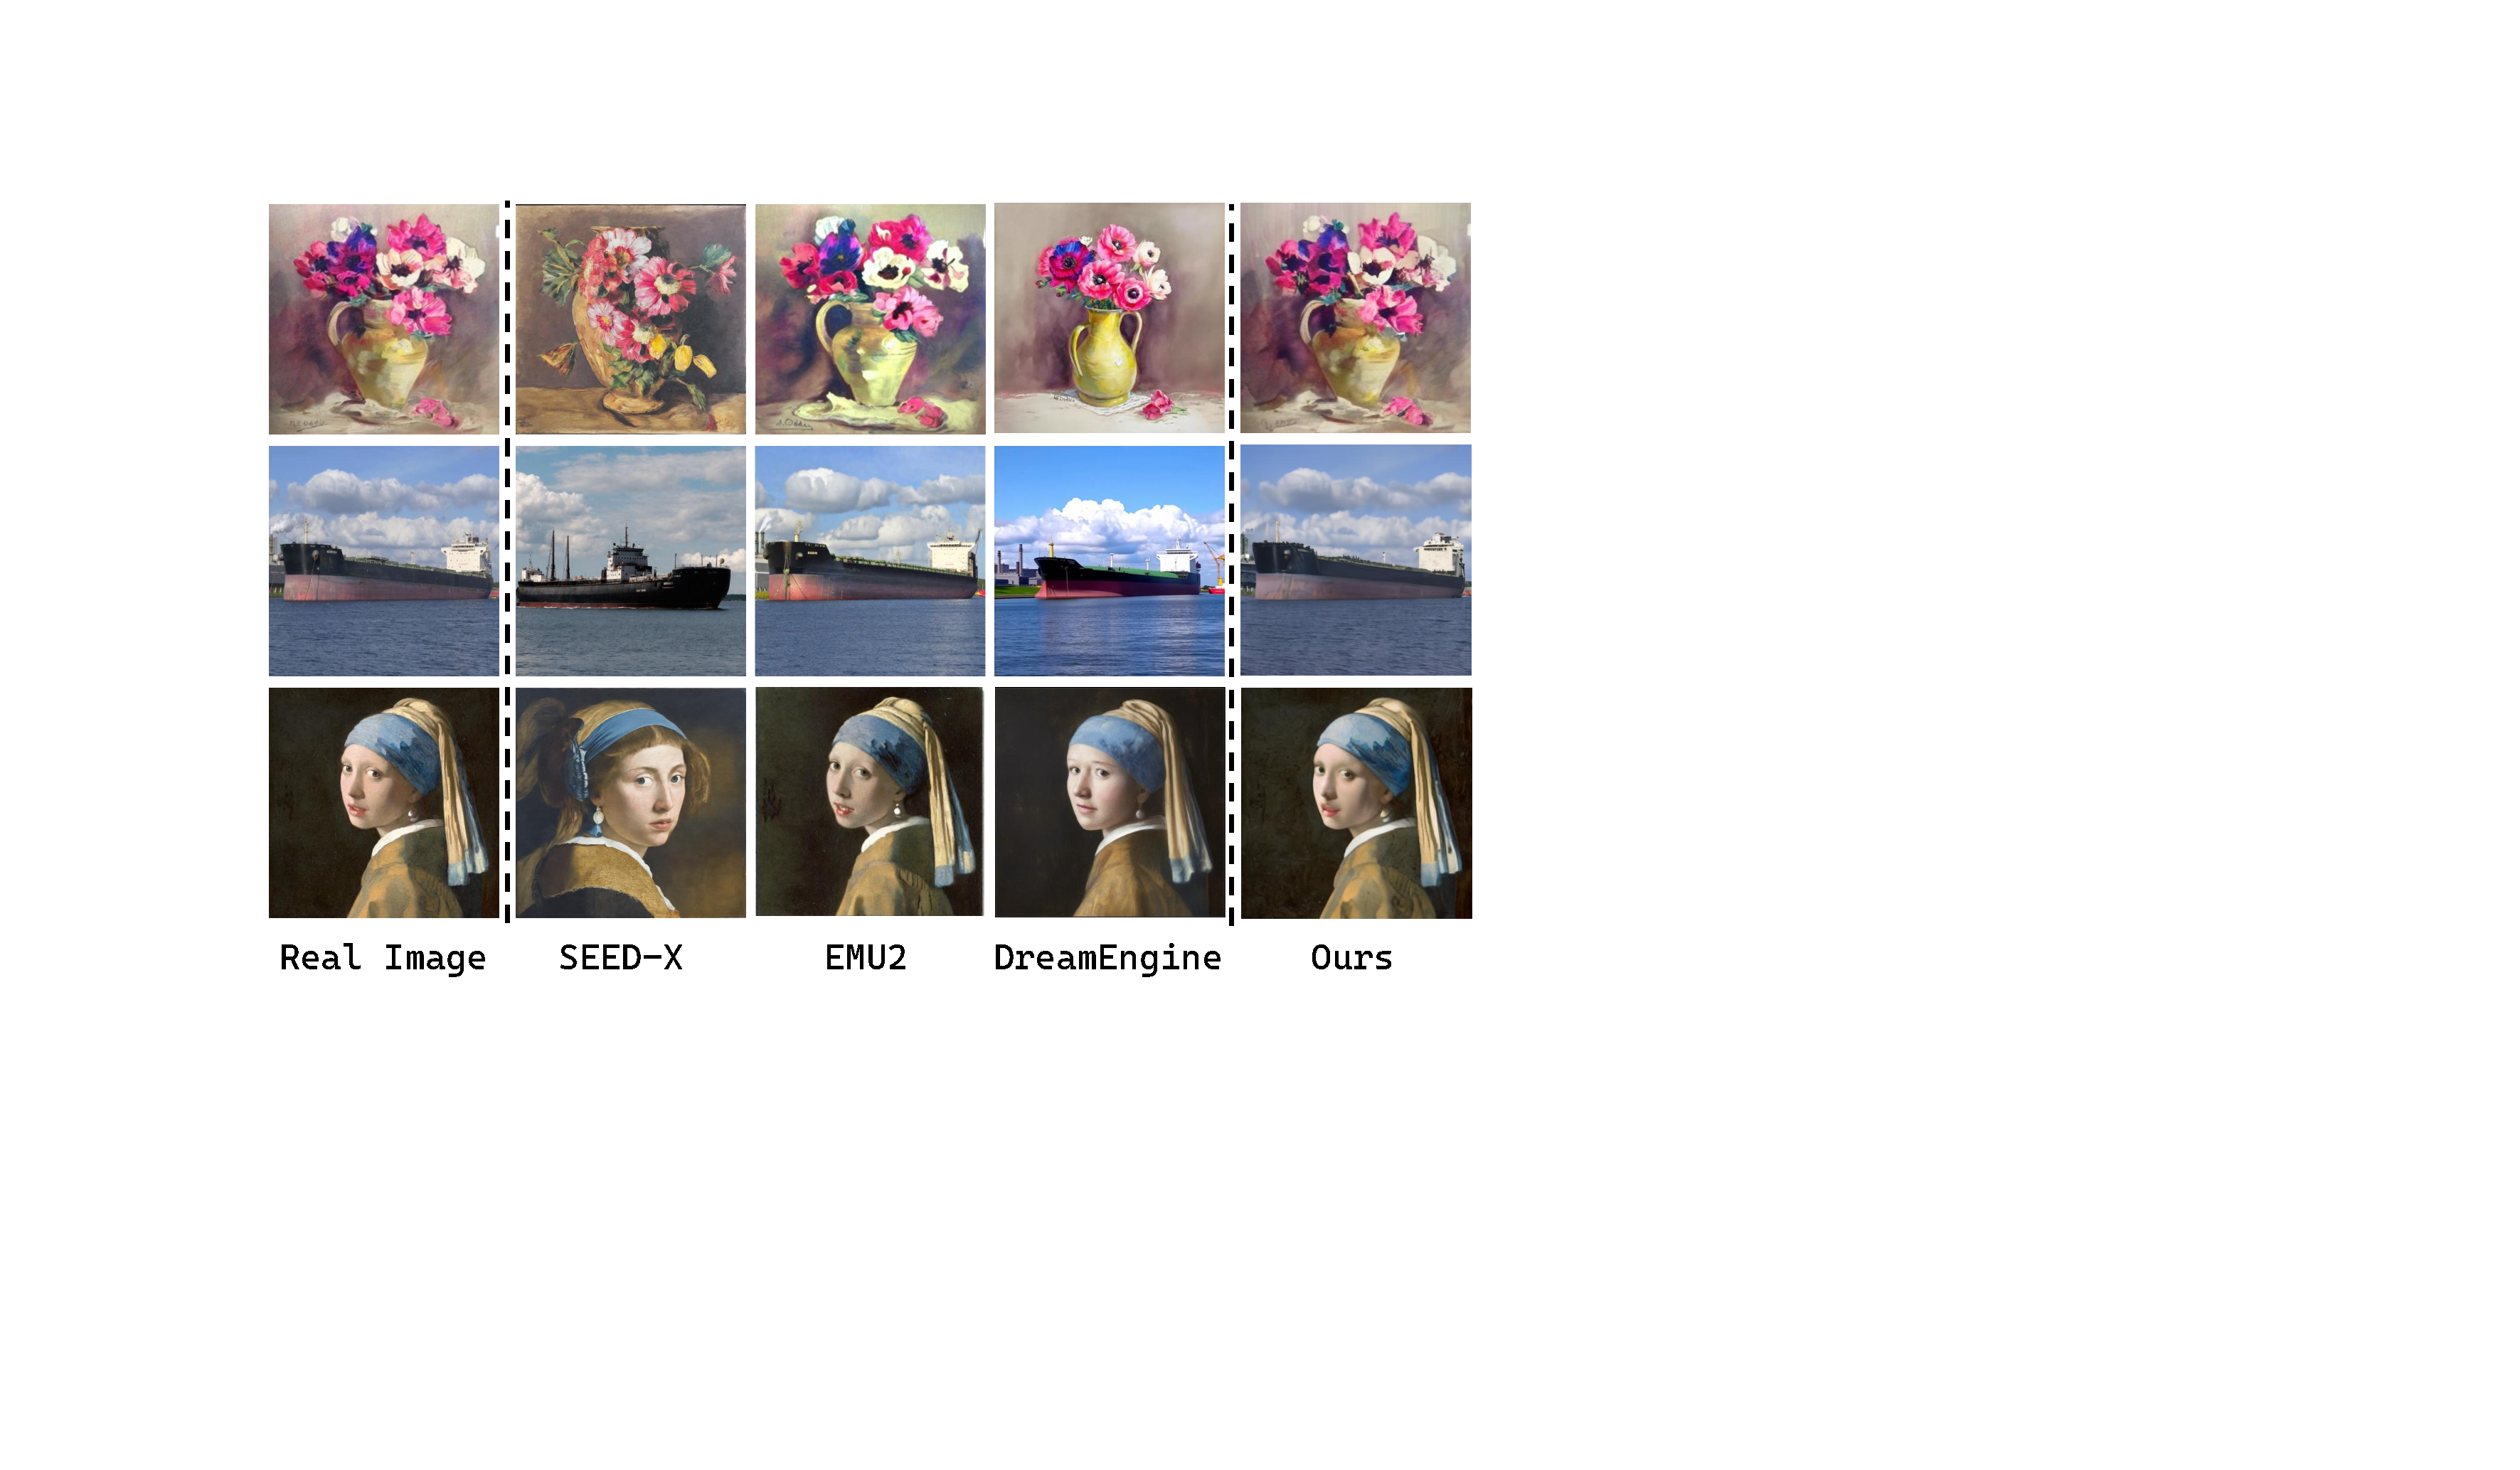
\includegraphics[width=\linewidth]{figures/reconstruction_exp.pdf}
        \vspace{-3ex}
        \captionof{figure}{Qualitative study on Image Reconstruction.}
        \label{fig:reconstruction}
    \end{minipage}
    \vspace{-5ex}

\end{wrapfigure}

\textbf{Image Reconstruction Fidelity.}
To quantify visual detail preservation in our framework, we evaluate \model on the Image Reconstruction Benchmark~\citep{dreamengine}, which measures similarity between input and reconstructed images. After fine‑tuning on reconstruction task for 1{,}000 steps, we compare the generated outputs with their originals using pixel‑space $\ell_2$ distance, following pervious work~\citep{dreamengine}. As shown in \Cref{tab:reconstruct_l2}, \model outperforms strong baselines with comparable architectures—SeedTokenizer~\citep{seed-tokenizer}, EMU2~\citep{emu2}, SeedX~\citep{2024SeedX}, and DreamEngine~\citep{dreamengine}—all of which couple LMMs with diffusion backbones.
\model achieves the best reconstruction quality, exceeding the second-best by 50\%, even with a $224{\times}224$ receptive field, while others varied from 384x384 to 512x512.
% In particular, it improves upon the second‑best approach by 51.2\% (COCO) and 57.7\%(JourneyDB) in $\ell_2$ distance, demonstrating superior pixel-level fidelity even with a $224{\times}224$ receptive field, while others range from 384x384 to 512x512. 
These gains confirm our model’s effectiveness at conditioning on—and faithfully reproducing—visual inputs.




% We introduce an  to evaluate the preservation of visual features in our Image-to-Image alignment task. This capability is essential for generating images conditioned on input images. 
% Afte finetuning on image reconstrction task for 1000 steps, we assess the similarity between the original and reconstructed images generatd by our model using the CLIP~\citep{radford2021clip} score and L2-Distance from the images in JourneyDB and COCO dataset. As shown in \Cref{tab:reconstruct}, we compare the performance of our model against several baselines with similar architectures, including SeedTokenizer~\citep{seed-tokenizer}, EMU-2~\citep{emu2}, SeedX~\citep{2024SeedX}, and DreamEngine~\citep{dreamengine}, which also integrate LMMs and diffusion models for generation. The results demonstrate that our model achieves the best average image reconstruction performance across both subsets of the benchmark. It notably surpasses the second-best by xx on the COCO and xx on the JourneyDB subsets in terms of L2 distance, highlighting its pixel-level consistency, albeit at an image receptive field of 224×224, while others varied from 384x384 to 512x512.


\textbf{Versatility Across Different Multimodal Tasks.}
To explore broader applicabilities of our framework, we evaluate its adaptability across diverse generation tasks, including image segmentation,  multi-image generation and multimodal in-context image generation. This was achieved with brief fine-tuning on relevant datasets, as detailed in~\Cref{app:applications}. Qualitative results in \Cref{fig:examples} show that the \model produces coherent, high-quality outputs that adhere to the provided constraints without requiring any architectural modifications. While achieving  performance in each specific domain would necessitate more specialized training and potentially more powerful multimodal encoder and generator components, these initial results underscore our framework's versatility and its potential as an effective foundation for a variety of multimodal conditional image generation applications.
 

% \paragraph{\mbox{Text-to-Image Generation}}

% We evaluate the text-to-image generation capability of our model on the COCO-40K benchmark. The results are presented in Table \ref{tab:fid_comparison}. Built upon the LlamaGen model~\citep{llamagen}, limited by the performance of the generator, our model shows much lower text-image generation ability than other baselines. However, thanks to the effective understanding of multimodal input, our model can balance these two different modalities, and with high-quality instruction following ability, ultimately further exceed other baselines in multimodal conditional image generation.
%  image segmentation set where? show cases additional task, editing; 



% \begin{table}[t]
% \centering
% \caption{Image reconstruction performance (L2 distance) on COCO and JourneyDB datasets.}
% \label{tab:reconstruct_l2}
% \resizebox{0.5\textwidth}{!}{
% \begin{tabular}{@{}lcc@{}}
% \toprule
% \textbf{Method} & \textbf{COCO ($\downarrow$)} & \textbf{JourneyDB ($\downarrow$)} \\
% \midrule
% SeedTokenizer              & 0.5102          & 0.5291          \\
% EMU2-Gen                  & 0.3828 & 0.2869 \\
% SEED-X                    & 0.4317          & 0.4352          \\
% DreamEngine               & \underline{0.2065}          & \underline{0.2052}          \\
% \midrule
% \textbf{Ours}             & \textbf{0.1008} & \textbf{0.0867} \\
% \bottomrule
% \end{tabular}
% }
% \end{table}



% \begin{figure*}[htbp]
% \centering
% 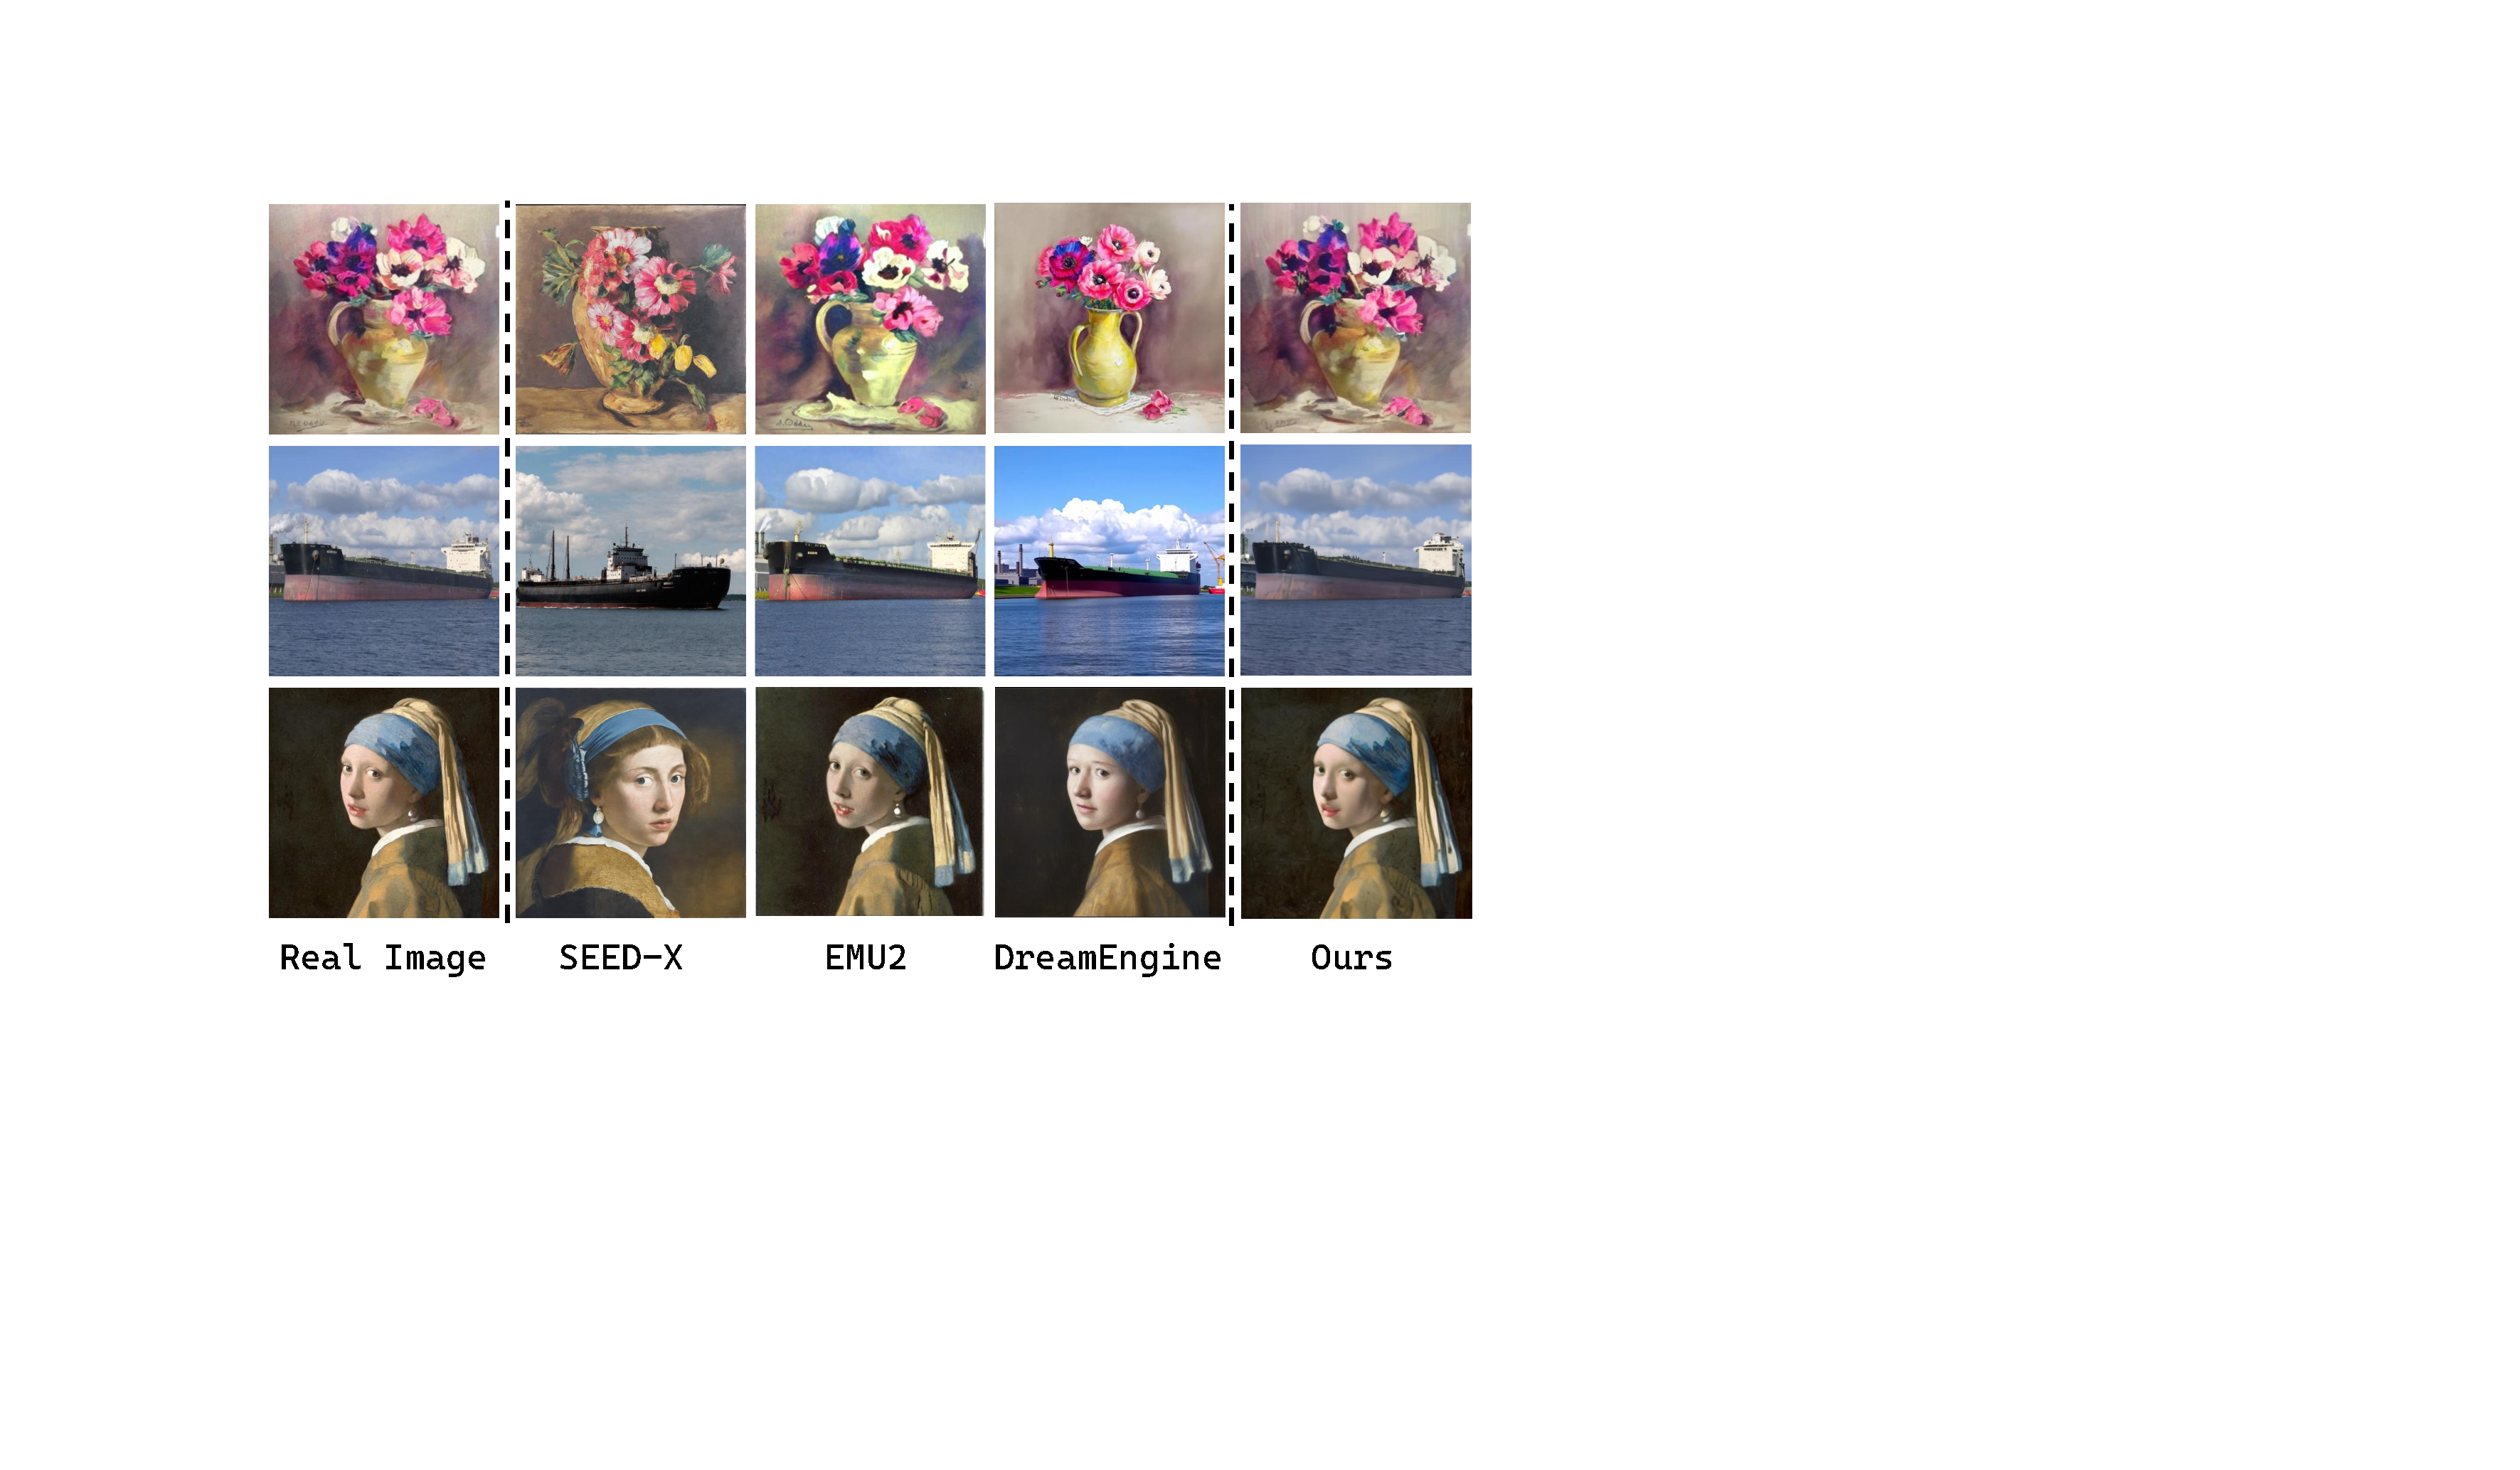
\includegraphics[width=1.0\textwidth]{figures/reconstruction_exp.pdf}
% \caption{Comparison of image reconstruction results among different methods~\citep{dreamengine,2024SeedX,emu2}.}
% \label{fig:reconstruction}
% \end{figure*}


% \begin{table}[t]
% \centering
% \caption{Image reconstruction performance comparison on COCO and JourneyDB datasets.}
% \label{tab:reconstruct}
% \resizebox{0.47\textwidth}{!}{
% \begin{tabular}{@{}lcccc@{}}
% \toprule
% \multirow{2}{*}{\textbf{Method}} & \multicolumn{2}{c}{\textbf{COCO}} & \multicolumn{2}{c}{\textbf{JourneyDB}} \\
% \cmidrule(lr){2-3} \cmidrule(lr){4-5}
%  & CLIP~($\uparrow$) & L2~($\downarrow$) & CLIP~($\uparrow$) & L2~($\downarrow$) \\
% \midrule
% SeedTokenizer              & 0.7760          & 0.5102          & 0.7921          & 0.5291 \\
% EMU2-Gen                  & 0.8537          & \underline{0.3828} & \textbf{0.9299} & \underline{0.2869} \\
% SEED-X                    & \underline{0.8595} & 0.4317          & 0.9017          & 0.4352 \\
% DreamEngine               & \textbf{0.8714} & 0.2065          & 0.9221          & 0.2052 \\

% \midrule
% Ours & 0.8335          & \textbf{0.1008}    & \underline{0.9062}   & \textbf{0.0867} \\
% \bottomrule
% \end{tabular}
% }
% \end{table}







% \paragraph{Image Segmentation}


% BLIP

% Llava

% Diffusion (Kosmos-G with our 1 stage training)


% \paragraph{Generation with Text-Image Interleaved Control}

% Upon completing Stage 2 training, our model gains the ability to integrate multimodal control within the image generation process. To assess our proposed paradigm of image generation capability under text-image interleaved control, we further train the model using a mixture of multi-image data. 

% In this paper, we demonstrate several applications of the model and evaluate its performance against Emu-2~\citep{emu2}, the most pertinent baseline which also facilitates text-image interleaved control.



\section{Related Work}
\label{sec:relatedwork}



% \begin{table}[htbp]
%   \centering
%   \setlength{\tabcolsep}{5pt}
%   \renewcommand{\arraystretch}{1.25}
%   \begin{tabular}{lccccccc}
%     \toprule
%     \textbf{Model} &
%     T$\Rightarrow$I &
%     I+T$\Rightarrow$T &
%     T+I$\Rightarrow$T+I &
%     Open-source &
%     Available &
%     \makecell[c]{Actual\\Support\\T+I$\Rightarrow$I} &
%     \makecell[c]{Within\\3 Month} \\
%     \midrule
%     EMU3              & \cmark & \cmark &        & \cmark & \cmark &        &        \\
%     LWM               & \cmark & \cmark &        & \cmark & \cmark & no train   &        \\
%     Unified-IO2       & \cmark & \cmark & ?      & \cmark & \cmark & \cmark &        \\
%     Lumina-mGPT       & \cmark & \cmark & \cmark & \cmark & \cmark & \cmark &        \\
%     Lumina-mGPT 2.0   & \cmark & \cmark & \cmark & \cmark &        &  no train   & \cmark \\
%     Liquid            & \cmark & \cmark &        & \cmark & \cmark & \cmark &        \\
%     vargpt            & \cmark & \cmark & ?      & \cmark & \cmark & ?      &        \\
%     vargpt-1.1        & \cmark & \cmark & \cmark & \cmark & \cmark & \cmark & \cmark \\
%     VILA-U            & \cmark &        & no train   & \cmark & \cmark & no train   &        \\
%     Janus             & \cmark & \cmark &        & \cmark & \cmark &        &        \\
%     MUSE-VL           & \cmark & \cmark &        &        &        &        &        \\
%     X-Prompt          & \cmark & \cmark & \cmark &        &        & \cmark &        \\
%     \bottomrule
%   \end{tabular}
%   \caption{Multimodal model capability and availability overview.}
%   \label{tab:model_overview}
% \end{table}



% \subsection{Image Generation with Complex Control}
% % blipdiffusion, kosmos-g, emu2, subject-diffusion, suti, control net
% Recent progress in controlled image generation using diffusion models has been significant. Researchers have explored various conditioning strategies—ranging from low-level cues like canny edges and depth maps~\citep{ye2023ip-adapter, controlnet} to higher-level guidance provided by reference images~\citep{SDEdit}—to steer the generative process. For instance, methods such as IP-Adapter~\citep{ye2023ip-adapter} and ControlNet~\citep{controlnet} incorporate additional control signals into standard text-to-image frameworks, thereby allowing more precise manipulation of generated content.
% In parallel, several works have leveraged visual elements from input images to further guide the generation process. DreamBooth~\citep{ruiz2023dreamboothfinetuningtexttoimage} and Textual Inversion~\citep{gal2022imageworthwordpersonalizing}, for example, adopt optimization-based approaches to adapt models to specific reference images. Although effective, these methods typically require extensive fine-tuning for each new input, limiting their practicality. To address these limitations, approaches like SuTI~\citep{suti} and Subject-diffusion~\citep{ma2024subjectdiffusionopendomainpersonalizedtexttoimage} have aimed to scale the fine-tuning process so that models can generalize across diverse reference images. However, these strategies still tend to be both time- and resource-intensive, highlighting the ongoing need for more efficient mechanisms for image generation with complex controls.

\subsection{Image Generation with Complex Multimodal Control}
Researchers have developed image generation via diffusion models conditioned on multimodal inputs like canny edges~\citep{controlnet} and reference images~\citep{ultraEdit,SDEdit}. ControlNet~\citep{controlnet} uses auxiliary parameters, while Mix-of-Show~\citep{Mix-of-Show} and FLUXSynID~\citep{FLUXSynID} use LoRA modules for multi-concept control and identity preservation.
DreamBooth~\citep{ruiz2023dreamboothfinetuningtexttoimage} enable subject-specific fine-tuning but limit generalization. SuTI~\citep{suti} address it with scalable data and training.
To enhance flexibility, recent work integrates LMMs with diffusion models by mapping LMM embedding into diffusion spaces~\citep{koh2023GILL,sun2023emu1,dreamllm,unimo}. Approaches like Kosmos-G~\citep{Kosmos-G}, Emu-2~\citep{emu2}, Seed-X~\citep{2024SeedX}, and DreamEngine~\citep{dreamengine} explore more complex multimodal prompt and fine-grained multimodal control. Yet, balancing guidance from diverse modalities remains a core challenge~\citep{han2024emmatexttoimagediffusionmodel,ye2023ip-adapter,RealCustom++}. 
EMMA~\citep{han2024emmatexttoimagediffusionmodel} employs a gated perceiver resampler for dynamic signal integration, while RealCustom++\citep{RealCustom++} disentangles subject identity and textual fidelity via cross-layer projectors. OmniControl~\citep{OminiControl} introduces a bias term into multimodal attention. 
Nonetheless, these method often require substantial computational resources, and achieving efficient, robust, and scalable multimodal integration remains an open problem.



\subsection{Autoregressive Multimodal Image Generation}
Autoregressive models have driven progress in T2I generation, from DALL·E~\cite{DALLE} and Parti~\citep{parti} to LlamaGen~\citep{llamagen} and GPT4O~\citep{gpt4o}.
Recent work extends it to multimodal settings: Models like Chameleon~\citep{chameleonteam2024chameleon}, LWM~\cite{LWM}, AnyGPT~\citep{Zhan2024AnyGPT}, and EMU3~\citep{Emu3} treat text and images as unified token sequences via early-fusion transformers, yet still emphasize text-to-image generation with limited support for multimodal conditioning.
Janus~\citep{Janus} decouples visual understanding and generation via distinct pathways, lacks support for multimodal image generation. MUSE-VL~\cite{musevl} and VILA-U~\citep{VILA-U}  align discrete visual tokens with text to improve perception, but remain oriented toward understanding tasks rather than image generation.
Unified-IO2~\citep{lu2023unifiedio2} is trained autoregressively from scratch for both understanding and generation across modalities, while Lumina-mGPT~\cite{2024lumina} enhances Chameleon with omnipotent supervised fine-tuning for broader multimodal tasks. Nonetheless, these models often over-rely on visual inputs while ignoring textual prompts.
Overall, while models like VILA-U~\cite{VILA-U}, EMU3~\cite{Emu3}, and Janus~\cite{Janus} have advanced text-to-image generation, robust multimodal conditional image generation remains an open and underexplored challenge.


\section{Conclusion}
\label{sec:conclusion}

In this work, we introduced a controllable and efficient autoregressive framework for complex multimodal image generation, offering a compelling alternative to diffusion-based methods.
By unifying multimodal inputs within an AR model and leveraging a two-stage training paradigm, our method achieves state-of-the-art performance on challenging benchmarks—despite a modest model size, suboptimal base component, and limited training resources.
These results underscore efficiency, scalability, and controllability of our method, establishing it as a efficient foundation for building versatile, fine-grained visual generation systems capable of handling complex multimodal prompts.

% By unifying multimodal inputs within AR framework and employing a two-stage training paradigm, our framework achieves state-of-the-art performance on complex benchmarks, demonstrating its efficiency, scalability, and controllability, even with a modest model size and significantly reduced training resources. This work establishes autoregressive models as a practical and scalable solution for multimodal image generation, laying a solid foundation for building versatile and controllable systems capable of nuanced visual generation from complex prompts.




% In this work, we have introduced an efficient and controllable autoregressive framework for complex multimodal image generation, effectively addressing the limitations inherent to diffusion-based methods. Our approach leverages a unified autoregressive transformer architecture that integrates visual and textual inputs into a shared latent representation, enabling precise token-level control and alignment without auxiliary adapters or cross-attention blocks. Crucially, our novel two-stage training paradigm—comprising a multimodal alignment stage and a multimodal instruction tuning stage—ensures robust multimodal alignment and balanced modality conditioning, achieving substantial improvements in generation fidelity and instruction adherence.
% Extensive experiments demonstrate our framework's superior performance, surpassing state-of-the-art diffusion models despite employing significantly smaller architectures and reduced training resources. Our results highlight the effectiveness and scalability of autoregressive models in multimodal image generation tasks, establishing them as viable alternatives to diffusion-based counterparts. 
% Moving forward, our methodology offers a promising foundation for developing efficient, versatile, and controllable multimodal generative systems, paving the way for broader applications requiring precise and nuanced visual generation from complex multimodal prompts.



\bibliography{ref}
\bibliographystyle{plainnat}

% \appendix

\section{DreamBench\texttt{++}: Benchmark Overview}
\label{app:DreamBench_Plus}

\paragraph{Data Organization.}  
DreamBench\texttt{++} comprises 150 high-quality reference images, sourced from Unsplash, Rawpixel, and Google Images, encompassing a balanced mix of subjects. These are evenly divided into three broad categories: \textit{objects}, \textit{living subjects} (humans and animals), and \textit{styles} (illustrative, painterly, etc.), ensuring visual and conceptual diversity.
In total, DreamBench\texttt{++} offers \textbf{1,350 prompts} ($150 \times 9$), representing a substantial scale-up over the original DreamBench (30 subjects $\times$ 25 prompts). Relative to DreamBench, the dataset is \textbf{5$\times$ larger in subjects} and \textbf{54$\times$ larger in prompts}, enabling broader evaluation of generative performance.

\paragraph{Evaluation Metric.}  
DreamBench\texttt{++} adopts an automatic, GPT-4o-based evaluation protocol designed to closely mirror human judgment. Each generated image is assessed against both its reference image and its corresponding prompt, using two complementary axes:

\begin{itemize}[left=2pt, itemsep=0.5pt,topsep=0.5pt]
  \item \textbf{Concept Preservation (CP):} Measures fidelity between the generated image and the reference. Key attributes include shape, color, texture, and facial details.
  \item \textbf{Prompt Following (PF):} Evaluates how well the generation aligns with the prompt in terms of relevance, accuracy, completeness, and contextual appropriateness.
\end{itemize}

Each axis is scored on a \textbf{five-level ordinal scale} from 0 (Very Poor) to 4 (Excellent), avoiding the complexity and bias of pairwise comparisons.



\section{Text-to-Image Generation Evaluation}

We evaluate text-to-image (T2I) generation performance on the MS-COCO~\citep{lin2014mscoco} and Geneval~\citep{2024Geneval} benchmarks to assess the generative capability of our model. Results are presented in \Cref{tab:fid_comparison} and \Cref{tab:exp-geneval}.
Since \model is built upon LLaMaGen, a relatively suboptimal generator, its standalone T2I performance is even weaker than ealy T2I models such as LDM and SD1.5. Unsurprisingly, models built on stronger generators—such as SDXL, SD3 like KOSMOS-G and Dream Engine demonstrate superior performance than ours.

However, despite its relatively limited T2I capacity, \model excels in multimodal image generation. Thanks to our proposed autoregressive architecture and two-stage multimodal-conditioned tuning strategy, \model effectively integrates both visual and textual signals during generation. This multimodal synergy simplifies the generation process and compensates for its weaker base generation capability, enabling \model to outperform stronger T2I models in multimodal settings, as demonstrated in \Cref{tab:comparison}. We expect that incorporating more powerful generators into \model would further enhance its performance. Nonetheless, our results indicate that \model is a promising and efficient alternative to diffusion-based approaches for multimodal image generation.


\begin{table*}[t]
    \centering
    \caption{GenEval benchmark results for text-to-image generation, classifying methods as either autoregressive or diffusion-based models. Due to our method's model size and suboptimal generators, we experience poor performance in text-to-image generation.}
    \resizebox{\textwidth}{!}{
    \begin{tabular}{@{}cl
        >{\centering\arraybackslash}m{1.4cm}
        >{\centering\arraybackslash}m{1.4cm}
        >{\centering\arraybackslash}m{1.4cm}
        >{\centering\arraybackslash}m{1.4cm}
        >{\centering\arraybackslash}m{1.4cm}
        >{\centering\arraybackslash}m{1.4cm}
        >{\centering\arraybackslash}m{1.4cm}
        @{}}
        \toprule
         & \textbf{Method} & \textbf{Single Object} & \textbf{Two Object} & \textbf{Counting} & \textbf{Colors} & \textbf{Position} & \textbf{Attribute Binding} & \textbf{Overall} \\
        \midrule

        \multirow{7}{*}{\rotatebox{90}{\textit{Autoregressive}}}
        & Chameleon~\cite{2024Chameleon}  & - & - & - & - & - & - & $0.39$ \\
        & LWM~\cite{2024LWM}  & $0.93$ & $0.41$ & $0.46$ & $0.79$ & $0.09$ & $0.15$ & $0.47$ \\
        & LlamaGen~\cite{2024llamagen} & $0.71$ & $0.34$ & $0.21$ & $0.58$ & $0.07$ & $0.04$ & $0.32$ \\
        & Show-o~\cite{2024Showo}  & $0.95$ & $0.52$ & $0.49$ & $0.82$ & $0.11$ & $0.28$ & $0.53$ \\
        & Emu$3$-Gen~\cite{2024emu3} & $0.98$ & $0.71$ & $0.34$ & $0.81$ & $0.17$ & $0.21$ & $0.54$ \\
        & Janus~\cite{2024Janus} & $0.97$ & $0.68$ & $0.30$ & $0.84$ & $0.46$ & $0.42$ & $0.61$ \\ 
        & \model & $0.87$ & $0.38$ & $0.18$ & $0.67$ & $0.08$ & $0.13$ & $0.38$ \\
        
        \midrule
        
        \multirow{12}{*}{\rotatebox{90}{\textit{Diffusion}}} 
        & LDM~\cite{2022LDM}  & $0.92$ & $0.29$ & $0.23$ & $0.70$ & $0.02$ & $0.05$ & $0.37$ \\
        & SDv$1.5$~\cite{2022LDM}  & $0.97$ & $0.38$ & $0.35$ & $0.76$ & $0.04$ & $0.06$ & $0.43$ \\
        & PixArt-$\alpha$~\cite{2023Pixelartalpha} & $0.98$ & $0.50$ & $0.44$ & $0.80$ & $0.08$ & $0.07$ & $0.48$ \\
        & SDv$2.1$~\cite{2022LDM} & $0.98$ & $0.51$ & $0.44$ & $0.85$ & $0.07$ & $0.17$ & $0.50$ \\
        & DALL-E~2~\cite{2022DALLE2} & $0.94$ & $0.66$ & $0.49$ & $0.77$ & $0.10$ & $0.19$ & $0.52$ \\
        & SDXL~\cite{2023SDXL} & $0.98$ & $0.74$ & $0.39$ & $0.85$ & $0.15$ & $0.23$ & $0.55$ \\
        & DALL-E~3~\cite{2023dalle3} & $0.96$ & $0.87$ & $0.47$ & $0.83$ & $0.43$ & $0.45$ & $0.67$ \\
        & SDv3 Medium~\cite{2024SD3} & $0.98$ & $0.74$ & $0.63$ & $0.67$ & $0.34$ & $0.36$ & $0.62$ \\
        & Flux.1 Dev~\citep{flux} & $0.98$ & $0.81$ & $0.74$ & $0.79$ & $0.22$ & $0.45$ & $0.66$ \\
        & Dream Engine~\citep{dreamengine} & $1.00$ & $0.94$ & $0.64$ & $0.81$ & $0.27$ & $0.49$ & $0.69$ \\
        & SDv3.5 Large~\cite{2024SD3} & $0.98$ & $0.89$ & $0.73$ & $0.83$ & $0.34$ & $0.47$ & $0.71$ \\

        \bottomrule
    \end{tabular}}
    \label{tab:exp-geneval}
\end{table*}

\begin{table}[t]
\centering
\begin{minipage}{0.30\textwidth}
\centering
\caption{Zero-shot FID comparisons on COCO.}
\label{tab:fid_comparison}
\resizebox{\textwidth}{!}{%
\begin{tabular}{@{}lc@{}}
\toprule
\textbf{Methods} & \textbf{FID} $\downarrow$ \\ \midrule
\multicolumn{2}{l}{\textit{T2I Models}} \\ 
GLIDE~\citep{GLIDE}        & 12.24 \\
Make-A-Scene~\citep{Make-a-Scene}    & 11.84 \\
DALL-E 2~\cite{2022DALLE2}      & 10.39 \\
SD v1.5 ~\cite{sd}       & 9.34  \\
Imagen~\citep{2022Imagen}    & 7.27  \\ \midrule
\multicolumn{2}{l}{\textit{CLIP-Aligned VL2I Models}} \\ 
GILL~\citep{koh2023GILL}         & 12.20 \\
Emu~\citep{sun2023emu1}     & 11.66 \\
KOSMOS-G~\citep{Kosmos-G}                 & 10.99 \\ \midrule
\model        & 19.92 \\ 
\bottomrule
\end{tabular}%
}
\end{minipage}%
\hfill
\begin{minipage}{0.68\textwidth}
\centering
\caption{Details on dataset used in the two-stage training.}
\label{tab:dataset}
\resizebox{\textwidth}{!}{
\begin{tabular}{@{}cllc@{}}
\toprule
\textbf{Stage} & \textbf{Data Source} & \textbf{Task} & \textbf{Number} \\
\midrule
\multirow{3}{*}{1} & Midjourney~\citep{midjourney-niji-1m-llavanext} & T2I & 700k \\
 & Midjourney~\citep{midjourney-niji-1m-llavanext} & Img Rec. & 180k \\
 & Synthetic Data & Obj. Sec.& 1.6M \\
\midrule
\multirow{4}{*}{2}  & Midjourney~\citep{midjourney-niji-1m-llavanext} \& Synthetic Data & T2I & 600k \\
 & Synthetic Data & Obj. Sec.  & 150k \\
 & Synthetic Data \& CC12M~\citep{changpinyo2021cc12m} & Img. Recov.  & 150k \\
 & Subject200k~\citep{OminiControl} & Sub. Gen.  & 400k \\
\bottomrule
\end{tabular}}
\end{minipage}
\end{table}


\section{Experimental Setup}
\label{app:exp_detail}


\subsection{Dataset Construction and Formation}
\label{app:data_form}

Table~\ref{tab:dataset} summarizes the datasets used in our two-stage training framework. Each stage is designed to progressively enhance distinct capabilities of the model using a diverse collection of multimodal data sources. In total, approximately 3 million samples are employed, with Stage 1 comprising around 2.5 million samples and Stage 2 involving 1.3 million samples, including an overlap of roughly 800k examples.
The dataset is constructed from a combination of open-source resources, such as Midjourney~\citep{midjourney-niji-1m-llavanext} and CC12M~\citep{changpinyo2021cc12m}, along with synthetic data generated via publicly available text-to-image (T2I) models, including Flux.1~\citep{flux} and Stable Diffusion v3.5~\citep{2024SD3}.

\textbf{Stage 1} focuses on establishing foundational multimodal alignment capabilities. Specifically, it includes 700k T2I samples from Midjourney~\citep{midjourney-niji-1m-llavanext}, 180k image reconstruction samples also from Midjourney, and 1.6M object segmentation samples generated through our pipeline.

\textbf{Stage 2} fine-tunes the model with 1.3 million samples. This includes 600k T2I samples—200k from Midjourney and 400k synthesized using open-source T2I models such as Flux.1~\citep{flux} and Stable Diffusion v3.5~\citep{2024SD3}. Additionally, we include 150k object segmentation samples and 150k image recovery samples, all derived from synthetic data using segmentation masks. Background images for the image recovery task are randomly selected from CC12M~\citep{changpinyo2021cc12m}.
We further incorporate 400k subject-driven image generation samples from Subject200k~\citep{OminiControl}. These samples are re-captioned using large multimodal models (LMMs) to extract subject-relevant text and generate comprehensive image descriptions. To enrich the training set, we reverse the input-output image pairs, effectively doubling the usable data to 400k samples.




\subsection{Implementation Details}
\label{app:imp_detail}

The multimodal encoder is initialized using vision encoder from CLIP-Large-Patch14~\citep{Radford2021LearningTV} and Flant5-XL-Encoder~\citep{flant5}, with an image receptive field of 224×224.
To implement the MLP-based Projection, we train the MLP Projector on LLaVA-CC3M-Pretrain-595K data~\citep{liu2023llava}, keeping the vision and text encode frozen following the setting of LLAVA alignment training. For the Query-based Token Distillation, the model is initialized with BLIP2-Flant5-XL~\citep{li2023blip2}.
The autoregressive generator is initialized from LlamaGen-XL~\citep{llamagen} with the size of 775M. The projector is a two-layer MLP featuring a middle projection dimension of 4,096 and employs SiLU as the activation function. 
The model is trained in two stages on 8 A100 GPUs, each with 80 GB of memory, taking approximately 1.5 days in total.

\subsection{Training Details}
\label{app:training_details}

In \textbf{Stage 1}, we freeze the multimodal encoder and train only the projector and generator modules for one epoch using a global batch size of 128. We adopt the Adam optimizer with an initial learning rate of 5e-4, apply linear warm-up over the first 5\% of total steps, and use a cosine decay schedule thereafter.

In \textbf{Stage 2}, we fine-tune the entire model except the vision encoder for two epochs. The learning rate is reduced to 1e-4, while all other optimization settings remain consistent with Stage 1. This stage focuses on enhancing cross-modal integration and improving the model’s ability to condition image generation on both visual and textual inputs.

For the ablation studies, we follow the same training schedule: one epoch on Stage 1 data, followed by two epochs on Stage 2 data.

In the \textbf{multi-image training} setting, we extend the context length of \model to 1280 tokens, allowing up to 4 images per context. We utilize 1.5 million multi-image samples, each containing multiple segmented sub-images and a corresponding caption. The model is tasked with reconstructing the original image from these segmented inputs and textual descriptions. To train this capability, we mix Stage 2 data with the multi-image data and train for an additional epoch.

Detailed training configurations and representative data examples are provided in the supplementary materials.


\section{Data Construction}
\label{app:data_construct}

To support the large-scale training required for our two-stage paradigm, we developed an automated pipeline for generating high-quality multimodal training data. This pipeline combines open-source image datasets with state-of-the-art vision-language models (VLMs) and segmentation models, enabling the construction of richly annotated image-text pairs with multiple segmented foreground objects without manual labeling:
% As depicted in \Cref{fig:data_pipeline}, the pipeline operates as follows:
\begin{itemize}[left=2pt]
    \item \textbf{Captioning and Object Extraction:} Query a VLM to generate a comprehensive caption describing prominent elements in the image and then extract a list of concrete, distinct, and segmentable objects. It ensures generated data focus on concrete visual objects.
    % This ensures downstream tasks focus on tangible visual entities.
    \item \textbf{Spatial Grounding:} For each extracted object, the VLM is queried again to identify its spatial location within the image, returning both a tight bounding box and several representative 2D keypoints. These spatial cues constrain the region of interest for subsequent segmentation, improving accuracy and reducing background noise.
    \item \textbf{Segmentation:} A segmentation model is employed to extract object masks from the image, guided by the generated bounding boxes and keypoints. This step produces high-quality masks that are both semantically aligned with the object labels and spatially accurate.
\end{itemize}
By applying this automated process to a large corpus of open-source images, we construct a diverse multimodal dataset comprising captioned images annotated with multiple precisely segmented objects. This dataset forms a critical component of our training setup, particularly enabling the object segmentation and image recovery tasks in our training paradigm.



% \section{KOSMOS-G Post-Training and Inference Details}
% \label{apx:video_model_details}

% For post-training during alignment tuning, we used the t2v-turbo-v1 codebase \cite{li2024t2v}, available at \url{https://github.com/Ji4chenLi/t2v-turbo}. A reward model loss scale of 1 was applied. The video model was jointly trained with both the reward model loss and the diffusion loss over 200 steps, using data sampled from the WebVideo dataset.

% For inference, we also utilized the same t2v-turbo-v1 codebase. Each inference setting was run 10 times with different random seed to ensure consistency and robustness of the results.



\section{Versatility Across Different Multimodal Tasks}
\label{app:applications}
To evaluate the broader applicability of our framework, we test its adaptability across diverse multimodal generation tasks, including image segmentation, subject-driven image generation, multi-image generation, and multimodal in-context image generation.
For each task, we perform supervised fine-tuning as needed. Specifically, for \textbf{image segmentation}, we evaluate the model directly after Stage 1 training. For \textbf{subject-driven image generation}, we use the model trained up to Stage 2 without additional fine-tuning.
For \textbf{multi-image generation}, we use the X2I dataset~\citep{OmniGen}, fine-tuning the Stage 2 model for two additional epochs. We manually split the dataset into training and test sets, ensuring no overlap between them. Quantitative results are reported on the test set.
For \textbf{multimodal in-context image generation}, we use the X2I-ICL dataset~\citep{OmniGen}, which focuses on in-context image segmentation tasks. We fine-tune the model for 10 epochs, again ensuring a strict train-test split with no overlap.
Qualitative results in \Cref{fig:examples} demonstrate that \model produces coherent, high-quality outputs that follow the provided constraints—without requiring any architectural modifications. Additional qualitative analyses and examples are included in the supplementary materials.



\section{Limitations}
\label{app:limitation}

Our work presents a promising alternative to diffusion-based methods for multimodal-conditioned image generation. As such, our focus is on evaluating performance under comparable conditions—i.e., with similar model capacities and training paradigms.
However, the effectiveness of our approach is currently constrained by the limitations of available autoregressive (AR) backbone models. Due to the lack of high-performance AR generators, \model exhibits shortcomings in several aspects of image generation, including spatial reasoning, object counting, fine-grained human rendering, and stylization. These limitations reflect the current gap between current SOTA diffusion and autoregressive architectures in terms of generation fidelity and domain generalization.
Additionally, while our training data is sourced from publicly available datasets and our synthetic data pipeline includes NSFW safeguards, a comprehensive evaluation of safety, fairness, and potential misuse remains lacking. Future work should incorporate thorough assessments of model biases and unintended behaviors.
Finally, while our framework demonstrates strong versatility across diverse multimodal tasks, achieving competitive performance in specific domains may require more specialized training and the integration of more powerful multimodal encoders and generators. These initial findings nonetheless highlight the framework's potential as a unified and efficient foundation for conditional multimodal image generation.


\clearpage
\appendix
\section{Technical Appendices and Supplementary Material}
\noindent This Supplementary Material is organized as follows.  

\begin{itemize}[left=0pt]
    \item In \Cref{sec:Exp_Details}, we provide the training details of \model, including initialization (\Cref{sec:init_Details}), training procedures (\Cref{sec:tra_Details}), and multi-image training strategy(\Cref{sub:multi_init_Details}).
    \item In \Cref{sup:t2i}, we show quantitative evaluations of our method on text-to-image generation benchmarks.
    \item In \Cref{sec:data_const}, we detail our data construction pipeline and the dataset details used across the two-stage training.
    \item In \Cref{sec:Experiment_Details}, we elaborate on the experimental setup, including datasets and metrics (\Cref{sec:Benchmark_Details}), as well as detailed descriptions of baseline methods(\Cref{sec:Baselines_Details}).
    \item In \Cref{sec:Qualitative_Study}, we present qualitative results that demonstrate the capabilities of \model in various settings, such as image reconstruction(\Cref{sec:Reconstruction}), segmentation(\Cref{sec:Segmentation}), multi-image generation(\Cref{sec:Multi-Image}), and in-context image generation(\Cref{sec:mmicl}).
    \item In \Cref{app:applications}, we demonstrate the versatility of \model across diverse multimodal generation tasks, including segmentation, subject-driven generation, and multimodal in-context learning.
    \item In \Cref{app:limitation}, we discuss the current limitations of our method, such as its dependence on autoregressive generators, generation fidelity, and safety considerations.
\end{itemize}


\section{Training Details}
\label{sec:Exp_Details}

\subsection{Initialization Details}
\label{sec:init_Details}

The multimodal encoder is initialized using the vision encoder from CLIP-Large-Patch14~\citep{Radford2021LearningTV}, with an image receptive field of $224 \times 224$, and the FlanT5-XL encoder~\citep{flant5}, with a context length of 512 tokens. This encoder converts each image into 256 tokens for use as context in the generator.

To implement the MLP-based projection, we train the MLP projector on the LLaVA-CC3M-Pretrain-595K dataset~\citep{liu2023llava}, following the alignment training setup used by LLaVA. Specifically, we freeze both the vision and text encoders (CLIP-Large-Patch14 and FlanT5-XL, respectively) and train only the MLP layers. The resulting pretrained MLP layers are then directly incorporated into the multimodal encoder of \model.


\begin{figure*}[htbp]
\centering
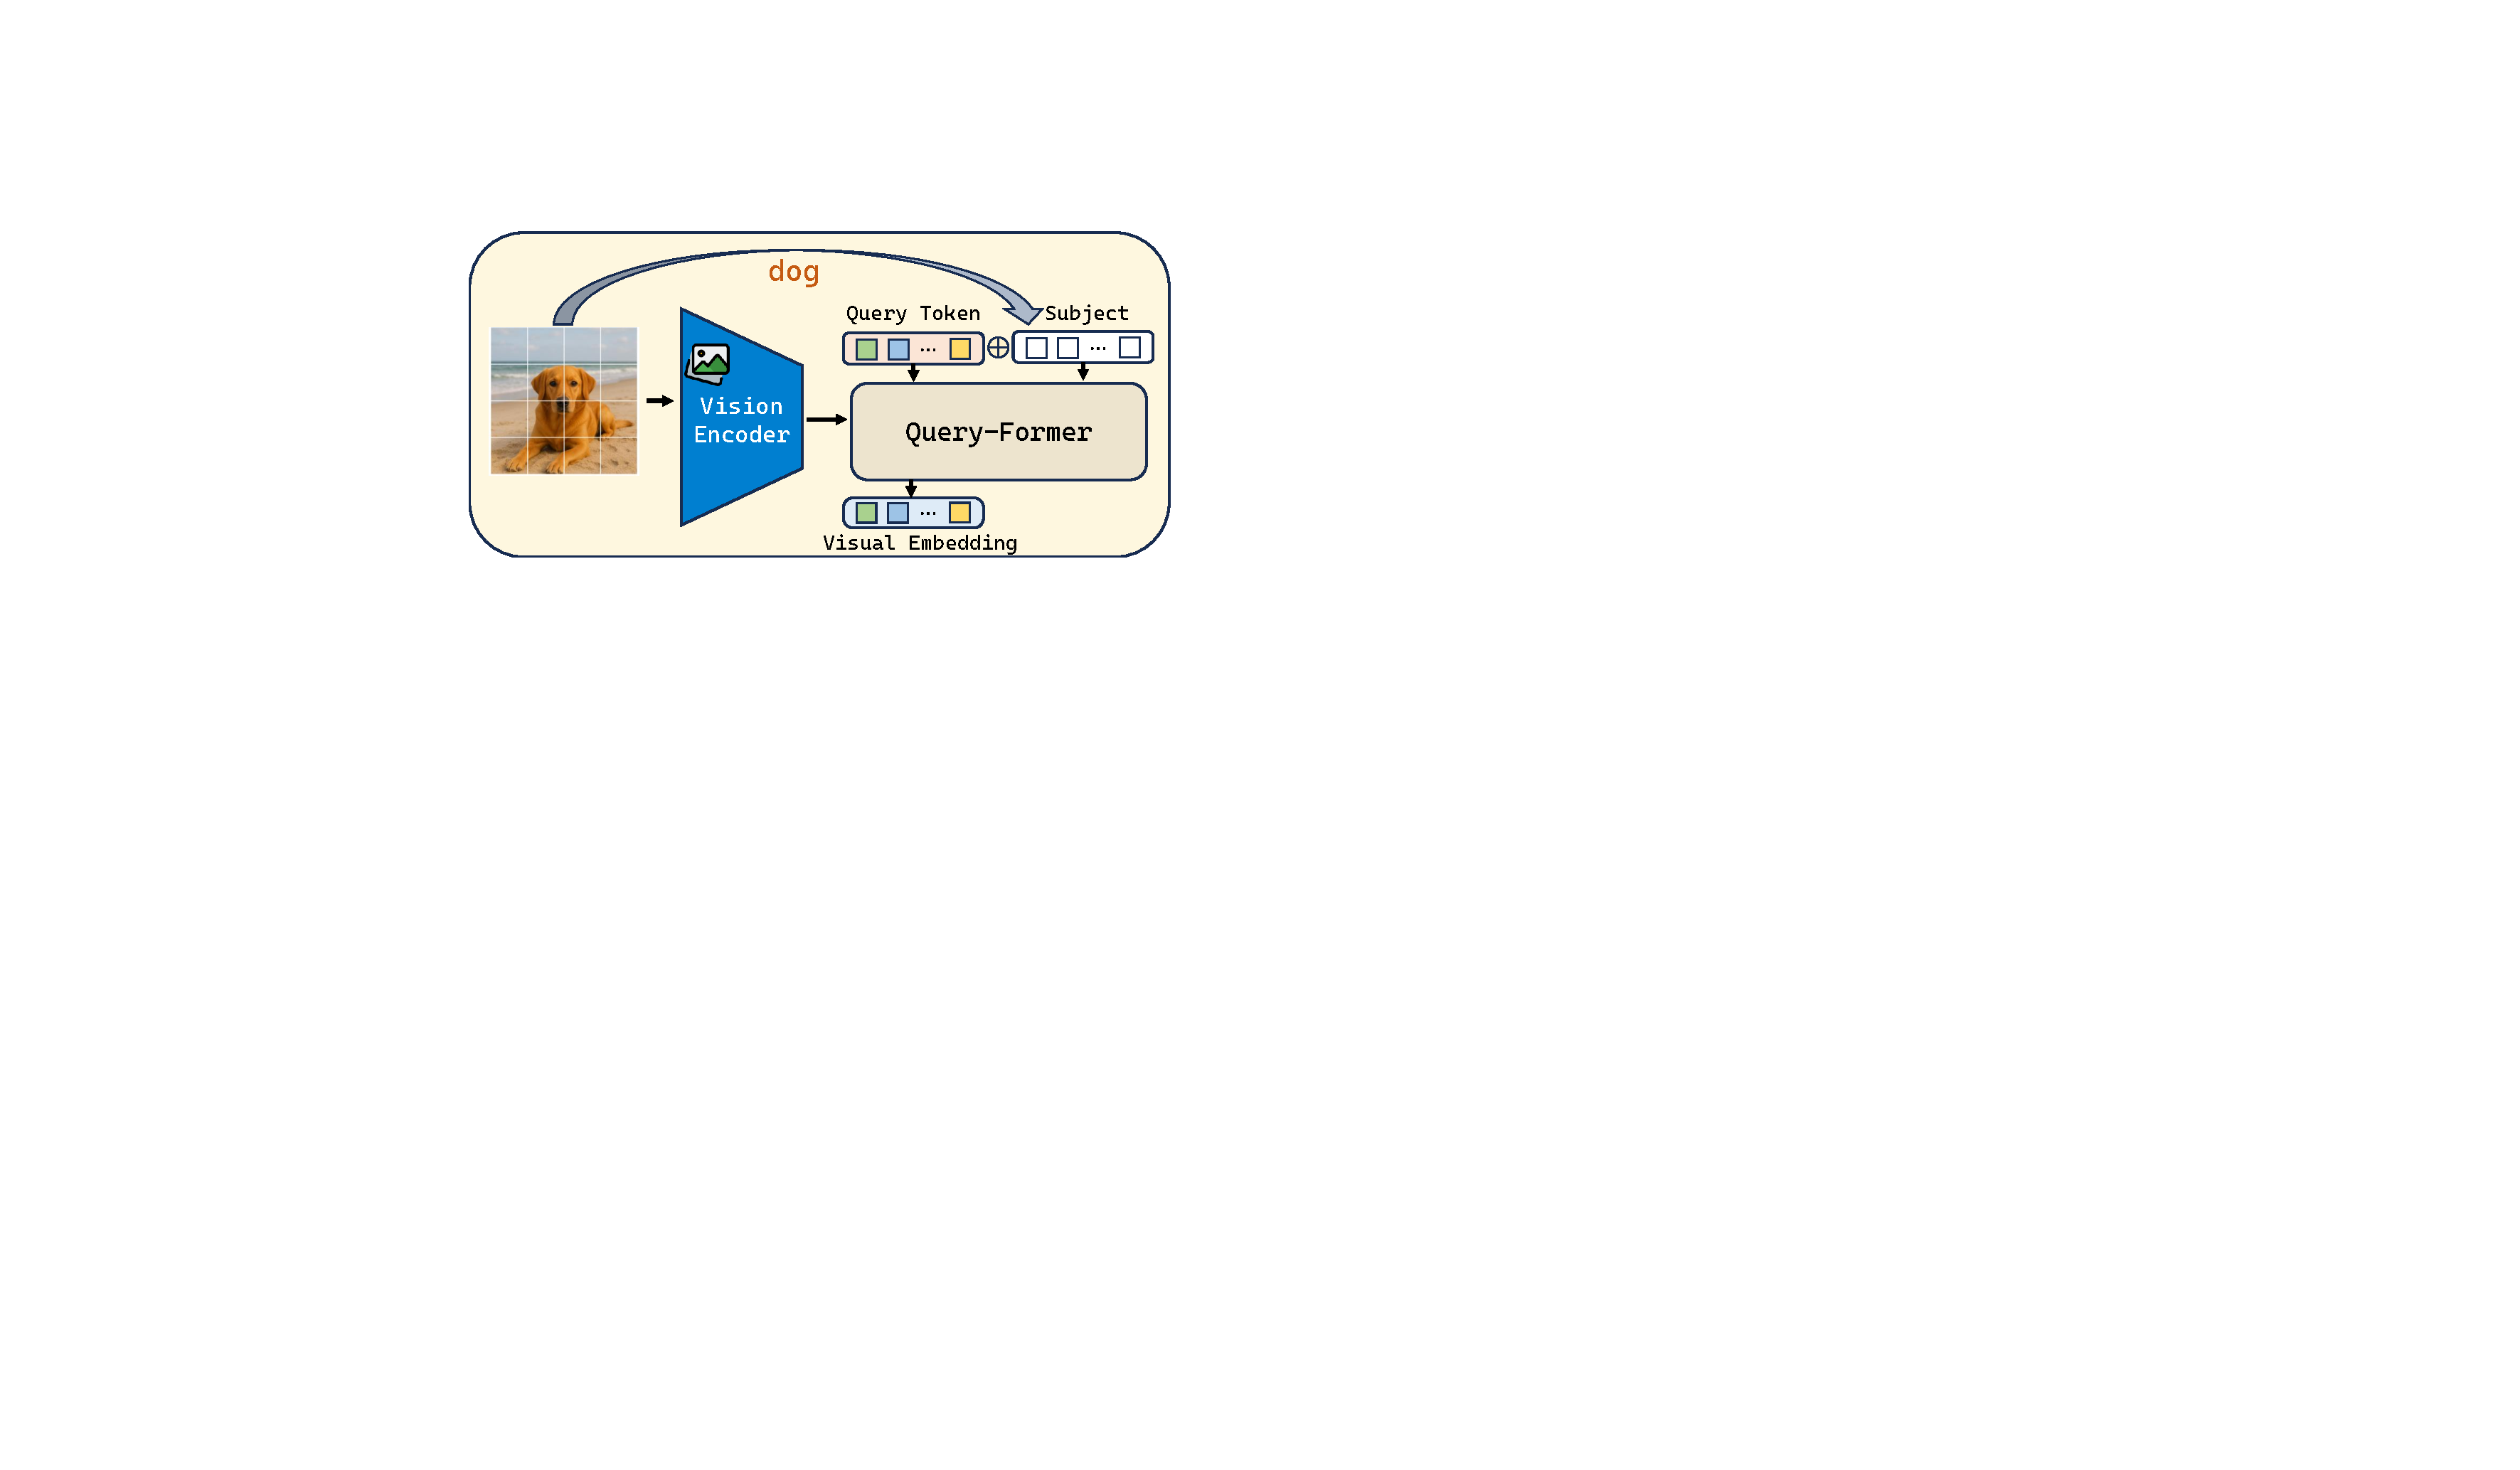
\includegraphics[width=0.8\textwidth]{figures/qformer.pdf}
\caption{Overview of text-guided visual distillation using the Query-based variant of \model.}
\label{fig:qformer}
\end{figure*}

The projector consists of a two-layer MLP with an intermediate dimension of 4,096, employing SiLU activation functions.
The autoregressive generator is initialized from LlamaGen-XL~\citep{llamagen} with 775 million parameters. 
However, the original LlamaGen implementation contains a fundamental error in its 2D Rotary Positional Embedding\citep{lu2023unifiedio2,EVA-02} (ROPE) mechanism\footnote{\url{https://github.com/FoundationVision/LlamaGen/issues/54}}, which leads to a loss of information in the query and key vectors during attention computation. To address this, we correct the ROPE implementation in our code and continue training the revised model on both the Midjourney dataset~\citep{midjourney-niji-1m-llavanext} and the LAION-COCO dataset used in LlamaGen pretraining, effectively replicating the original pretraining conditions. This continued training enables the model to adapt to the corrected ROPE mechanism. The resulting model is then used to initialize our autoregressive generator.

\subsection{Training Procedure}
\label{sec:tra_Details}

The model training comprises two distinct stages:

\textbf{Stage 1}: We freeze the multimodal encoder and train only the projector and generator modules for one epoch, using a global batch size of 128. Optimization employs the Adam optimizer with an initial learning rate of $5 \times 10^{-4}$, a linear warm-up over the initial 5% of steps, and a subsequent cosine decay schedule.

\textbf{Stage 2}: We fine-tune the entire model, excluding the vision encoder, for two epochs. The learning rate is reduced to $1 \times 10^{-4}$, with all other optimization settings remaining consistent with Stage 1. This phase primarily enhances cross-modal interactions and improves conditional image generation capabilities from combined visual and textual inputs.

Training is conducted across 8 NVIDIA A100 GPUs, each equipped with 80 GB memory, taking approximately 1.5 days. Specifically, Stage 1 training involves 2.48 million data points over a single epoch, completed in roughly 14 hours. Stage 2 training utilizes 1.3 million data points over two epochs, taking approximately 20 hours in total.

Ablation studies follow the same training schedule, with one epoch of training on Stage 1 data, followed by two epochs on Stage 2 data.

\subsection{Multi-Image Training}
\label{sub:multi_init_Details}
In \textbf{multi-image training} scenario, the context length of \model is expanded to 1,280 tokens to accommodate up to 4 images per context. For the Query-based variant of \model, token compression techniques enable processing up to 14 images per context with 512 context length.

We utilize 1.5 million multi-image samples, each comprising segmented sub-images accompanied by textual descriptions. The model is trained to reconstruct original images based on these segmented inputs and their corresponding captions. Training incorporates a mixture of Stage 2 data and multi-image samples for an additional epoch.

Qualitative assessments, presented in \Cref{fig:multi}, demonstrate that multi-image training significantly enhances the model's capability to preserve detailed visual information in complex multimodal contexts.

\begin{figure*}[t]
\centering
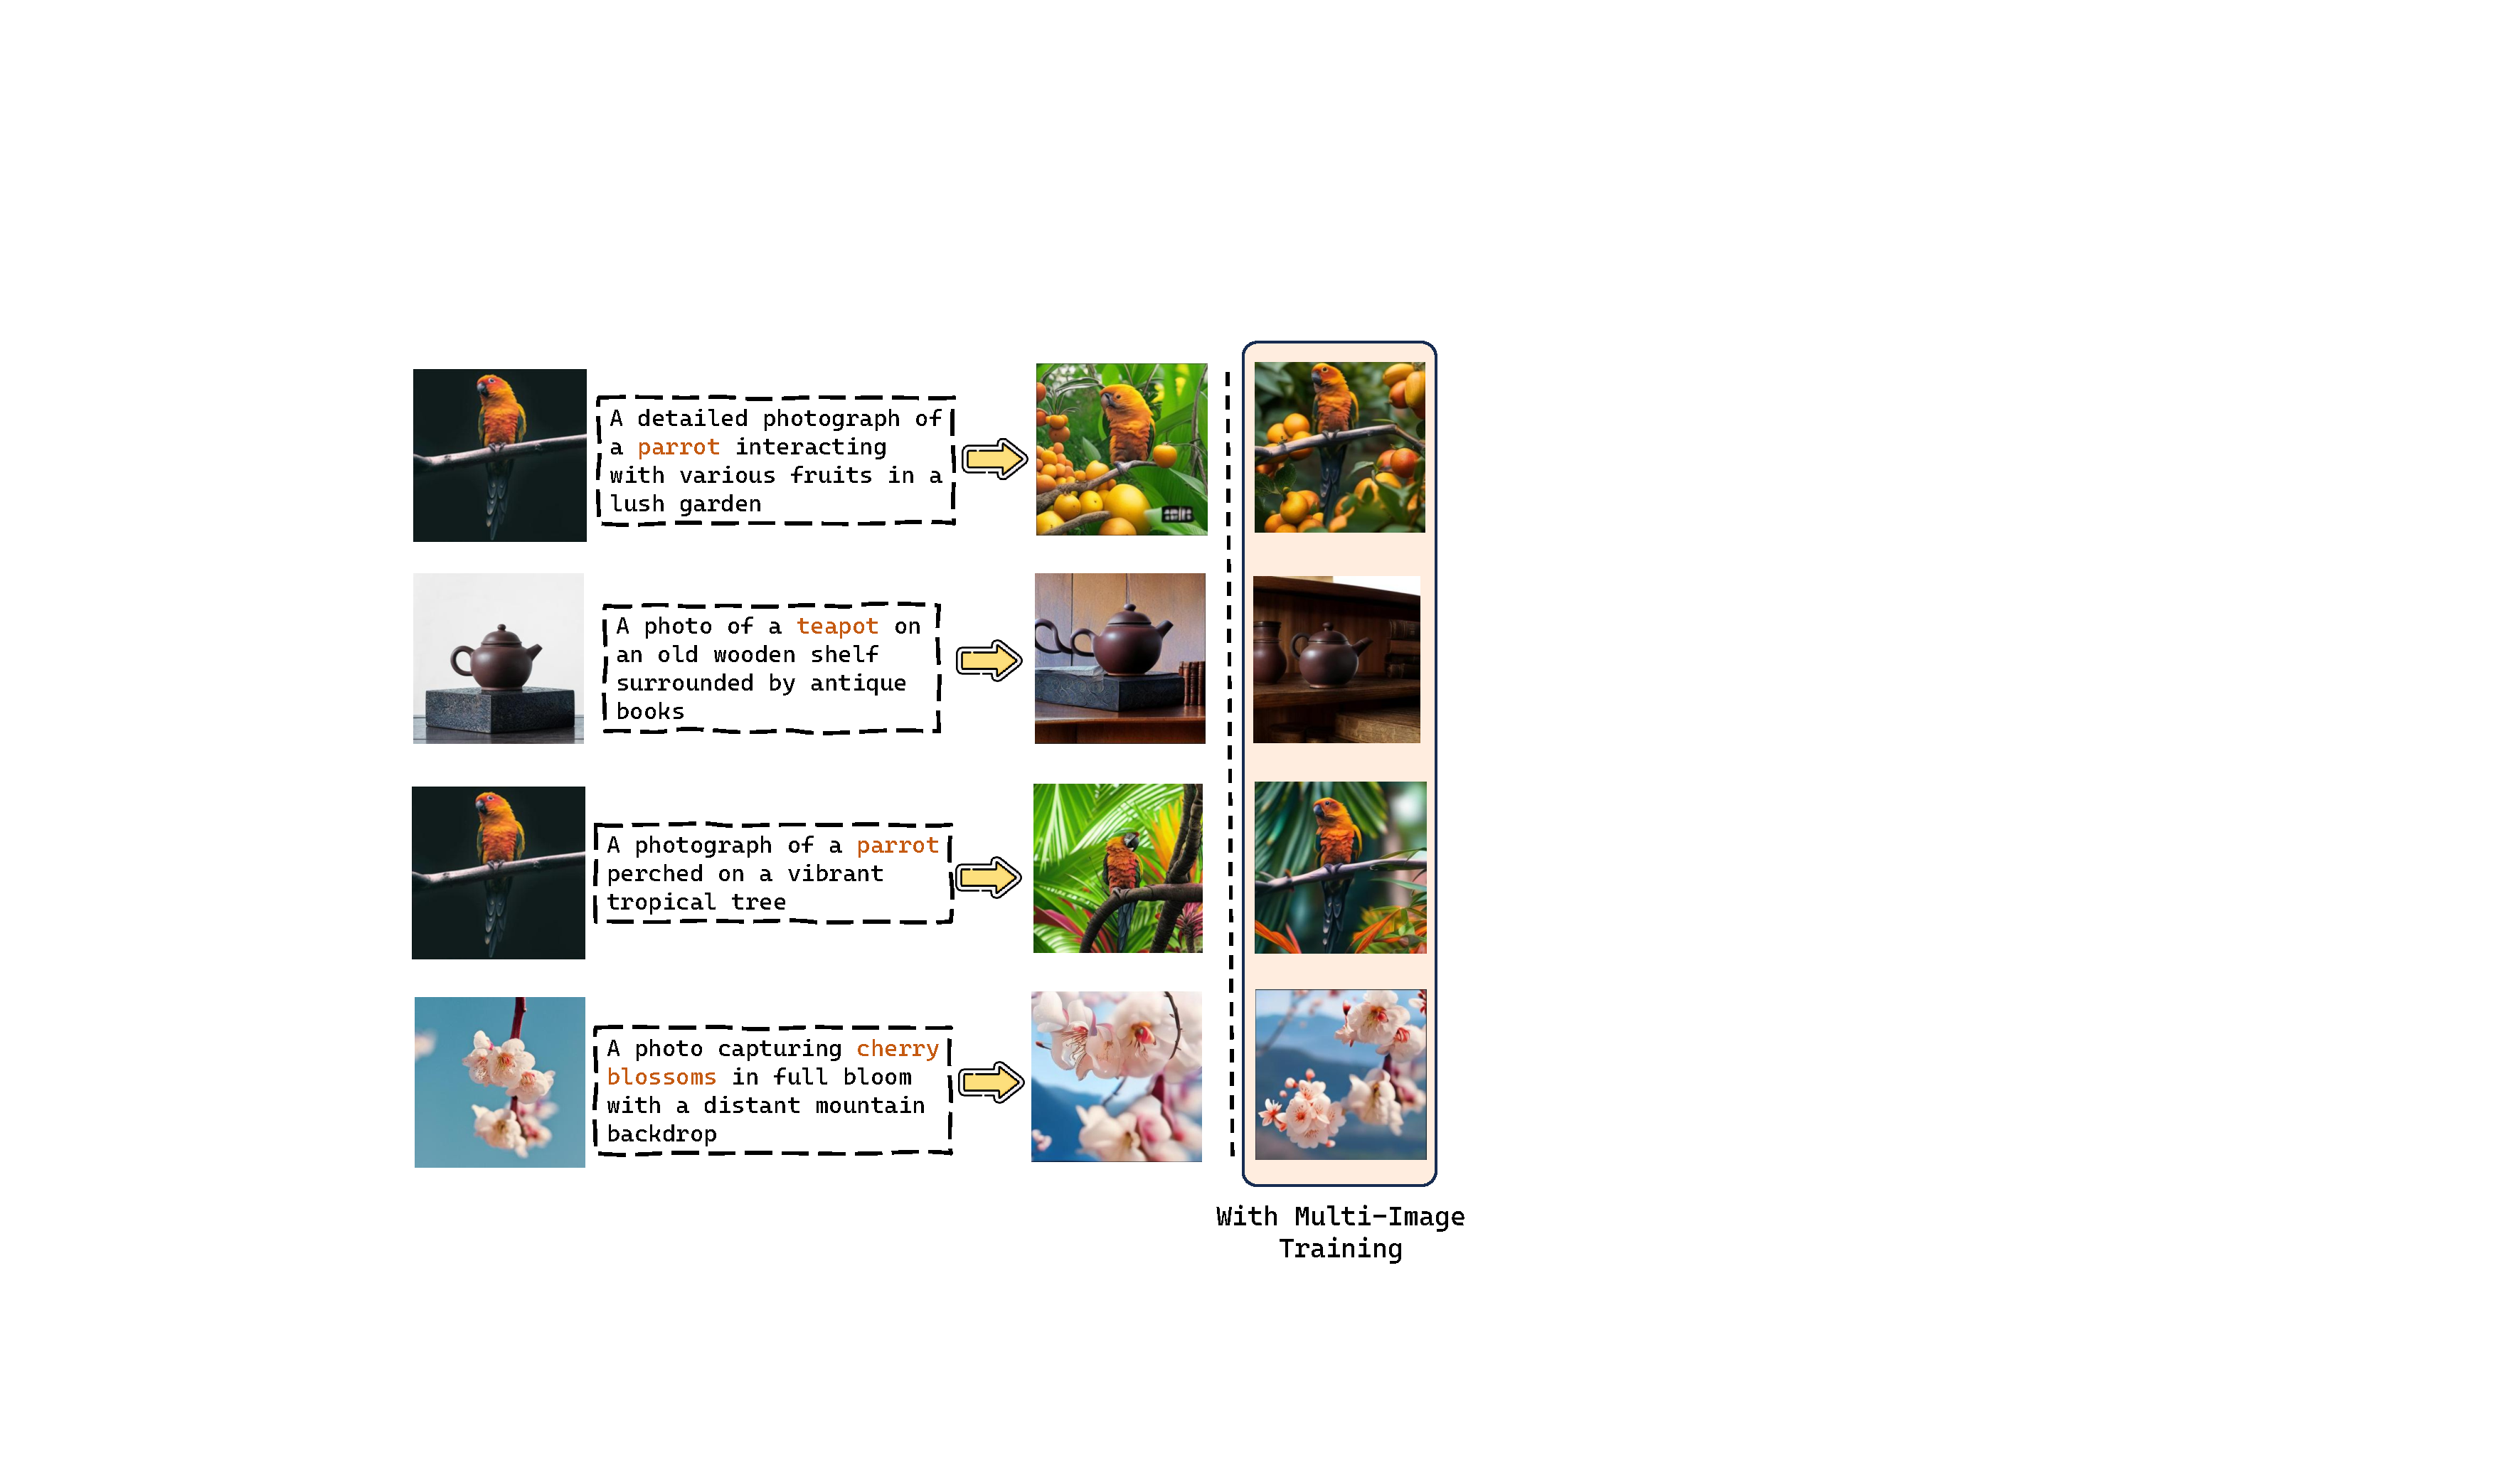
\includegraphics[width=1.0\textwidth]{figures/multi_exp.pdf}
\caption{Qualitative assessment demonstrating improved preservation of visual details by \model following multi-image training.}
\label{fig:multi}
\end{figure*}

\section{Text-to-Image Generation Evaluation}
\label{sup:t2i}
\begin{table*}[t]
    \centering
    \caption{GenEval benchmark results for text-to-image generation, classifying methods as either autoregressive or diffusion-based models. Due to our method's model size and suboptimal generators, we experience poor performance in text-to-image generation.}
    \resizebox{\textwidth}{!}{
    \begin{tabular}{@{}cl
        >{\centering\arraybackslash}m{1.4cm}
        >{\centering\arraybackslash}m{1.4cm}
        >{\centering\arraybackslash}m{1.4cm}
        >{\centering\arraybackslash}m{1.4cm}
        >{\centering\arraybackslash}m{1.4cm}
        >{\centering\arraybackslash}m{1.4cm}
        >{\centering\arraybackslash}m{1.4cm}
        @{}}
        \toprule
         & \textbf{Method} & \textbf{Single Object} & \textbf{Two Object} & \textbf{Counting} & \textbf{Colors} & \textbf{Position} & \textbf{Attribute Binding} & \textbf{Overall} \\
        \midrule

        \multirow{7}{*}{\rotatebox{90}{\textit{Autoregressive}}}
        & Chameleon~\cite{2024Chameleon}  & - & - & - & - & - & - & $0.39$ \\
        & LWM~\cite{2024LWM}  & $0.93$ & $0.41$ & $0.46$ & $0.79$ & $0.09$ & $0.15$ & $0.47$ \\
        & LlamaGen~\cite{2024llamagen} & $0.71$ & $0.34$ & $0.21$ & $0.58$ & $0.07$ & $0.04$ & $0.32$ \\
        & Show-o~\cite{2024Showo}  & $0.95$ & $0.52$ & $0.49$ & $0.82$ & $0.11$ & $0.28$ & $0.53$ \\
        & Emu$3$-Gen~\cite{2024emu3} & $0.98$ & $0.71$ & $0.34$ & $0.81$ & $0.17$ & $0.21$ & $0.54$ \\
        & Janus~\cite{2024Janus} & $0.97$ & $0.68$ & $0.30$ & $0.84$ & $0.46$ & $0.42$ & $0.61$ \\ 
        & \model & $0.87$ & $0.38$ & $0.18$ & $0.67$ & $0.08$ & $0.13$ & $0.38$ \\
        
        \midrule
        
        \multirow{12}{*}{\rotatebox{90}{\textit{Diffusion}}} 
        & LDM~\cite{2022LDM}  & $0.92$ & $0.29$ & $0.23$ & $0.70$ & $0.02$ & $0.05$ & $0.37$ \\
        & SDv$1.5$~\cite{2022LDM}  & $0.97$ & $0.38$ & $0.35$ & $0.76$ & $0.04$ & $0.06$ & $0.43$ \\
        & PixArt-$\alpha$~\cite{2023Pixelartalpha} & $0.98$ & $0.50$ & $0.44$ & $0.80$ & $0.08$ & $0.07$ & $0.48$ \\
        & SDv$2.1$~\cite{2022LDM} & $0.98$ & $0.51$ & $0.44$ & $0.85$ & $0.07$ & $0.17$ & $0.50$ \\
        & DALL-E~2~\cite{2022DALLE2} & $0.94$ & $0.66$ & $0.49$ & $0.77$ & $0.10$ & $0.19$ & $0.52$ \\
        & SDXL~\cite{2023SDXL} & $0.98$ & $0.74$ & $0.39$ & $0.85$ & $0.15$ & $0.23$ & $0.55$ \\
        & DALL-E~3~\cite{2023dalle3} & $0.96$ & $0.87$ & $0.47$ & $0.83$ & $0.43$ & $0.45$ & $0.67$ \\
        & SDv3 Medium~\cite{2024SD3} & $0.98$ & $0.74$ & $0.63$ & $0.67$ & $0.34$ & $0.36$ & $0.62$ \\
        & Flux.1 Dev~\citep{flux} & $0.98$ & $0.81$ & $0.74$ & $0.79$ & $0.22$ & $0.45$ & $0.66$ \\
        & Dream Engine~\citep{dreamengine} & $1.00$ & $0.94$ & $0.64$ & $0.81$ & $0.27$ & $0.49$ & $0.69$ \\
        & SDv3.5 Large~\cite{2024SD3} & $0.98$ & $0.89$ & $0.73$ & $0.83$ & $0.34$ & $0.47$ & $0.71$ \\

        \bottomrule
    \end{tabular}}
    \label{tab:exp-geneval}
\end{table*}

We evaluate the performance of our model on text-to-image (T2I) generation using the MS-COCO~\citep{lin2014mscoco} and GenEval~\citep{2024Geneval} benchmarks. Results are reported in \Cref{tab:fid_comparison} and \Cref{tab:exp-geneval}.

Since \model is built upon LLaMaGen—a relatively weaker autoregressive generator—its standalone T2I performance is inferior to earlier diffusion-based models such as LDM and SDv1.5. This is expected, as models based on more advanced generators (e.g., SDXL, SD3) such as KOSMOS-G and Dream Engine consistently outperform ours in conventional T2I metrics.

Nevertheless, \model demonstrates strong performance in multimodal image generation tasks. Thanks to our proposed autoregressive architecture and a two-stage multimodal-conditioned tuning strategy, \model effectively integrates both visual and textual modalities during generation. This synergistic design compensates for its weaker generation core, enabling \model to surpass more powerful T2I models in multimodal settings, as shown in \Cref{tab:comparison}. We anticipate that incorporating stronger base generators will further improve performance. Despite its current limitations, our results suggest that \model presents a promising and efficient alternative to diffusion-based methods in multimodal scenarios.

\begin{table}[t]
    \centering
    \caption{Zero-shot FID scores on the MS-COCO benchmark. Lower is better.}
    \label{tab:fid_comparison}
    \resizebox{0.35\textwidth}{!}{%
    \begin{tabular}{@{}lc@{}}
        \toprule
        \textbf{Model} & \textbf{FID} $\downarrow$ \\
        \midrule
        \multicolumn{2}{l}{\textit{T2I Models}} \\
        GLIDE~\citep{GLIDE}            & 12.24 \\
        Make-A-Scene~\citep{Make-a-Scene}     & 11.84 \\
        DALL-E 2~\citep{2022DALLE2}         & 10.39 \\
        SD v1.5~\citep{sd}             & 9.34  \\
        Imagen~\citep{2022Imagen}        & 7.27  \\
        \midrule
        \multicolumn{2}{l}{\textit{CLIP-Aligned VL2I Models}} \\
        GILL~\citep{koh2023GILL}           & 12.20 \\
        Emu~\citep{sun2023emu1}           & 11.66 \\
        KOSMOS-G~\citep{Kosmos-G}         & 10.99 \\
        \midrule
        \model                             & 19.92 \\
        \bottomrule
    \end{tabular}%
    }
\end{table}


\section{Data Construction and Formation}
\label{sec:data_const}

\begin{table}[!htbp]
\centering
\caption{Details on dataset used in the two-stage training.}
\label{tab:dataset1}
\small % Reduce font size
\begin{tabular}{@{}cllc@{}}
\toprule
\textbf{Stage} & \textbf{Data Source} & \textbf{Task} & \textbf{Number of Samples} \\ 
\midrule
\multirow{3}{*}{1} 
    & Midjourney\citep{midjourney-niji-1m-llavanext} & Text to Image Generation & 700k \\ 
    & Midjourney\citep{midjourney-niji-1m-llavanext} & Image Reconstruction & 180k \\ 
    & Synthetic Data & Object Segmentation & 1.6M \\ 
\midrule
\multirow{4}{*}{2} 
    & Midjourney\citep{midjourney-niji-1m-llavanext}, Synthetic Data & Text to Image Generation & 600k \\ 
    & Synthetic Data & Object Segmentation & 150k \\ 
    & Synthetic Data, CC12M\citep{changpinyo2021cc12m} & Image Recovery & 150k \\ 
    & Subject200k\citep{OminiControl} & Subject-driven Generation & 400k \\ 
\bottomrule
\end{tabular}
\end{table}


\paragraph{Data Formation}
Table~\ref{tab:dataset1} summarizes the datasets utilized in our two-stage training framework. Each stage is designed to progressively enhance distinct capabilities of the model using a diverse collection of multimodal data sources. In total, approximately 3 million samples are employed, with Stage 1 comprising around 2.5 million samples and Stage 2 involving 1.3 million samples, including an overlap of roughly 800k examples.

The dataset is constructed from a combination of open-source resources, such as Midjourney~\citep{midjourney-niji-1m-llavanext} and CC12M~\citep{changpinyo2021cc12m}, along with synthetic data generated via publicly available text-to-image (T2I) models, including Flux.1~\citep{flux} and Stable Diffusion v3.5~\citep{2024SD3}.

\textbf{Stage 1} focuses on establishing foundational multimodal alignment capabilities. Specifically, it includes 700k T2I samples from Midjourney~\citep{midjourney-niji-1m-llavanext}, 180k image reconstruction samples also from Midjourney, and 1.6M object segmentation samples generated through our pipeline.

\textbf{Stage 2} fine-tunes the model with 1.3 million samples. This includes 600k T2I samples—200k from Midjourney and 400k synthesized using open-source T2I models such as Flux.1~\citep{flux} and Stable Diffusion v3.5~\citep{2024SD3}. Additionally, we include 150k object segmentation samples and 150k image recovery samples, all derived from synthetic data using segmentation masks. Background images for the image recovery task are randomly selected from CC12M~\citep{changpinyo2021cc12m}.

We further incorporate 400k subject-driven image generation samples from Subject200k~\citep{OminiControl}. These samples are re-captioned using Qwen2-VL~\citep{Qwen2vl} to extract subject-relevant text and generate comprehensive image descriptions. To enrich the training set, we reverse the input-output image pairs, effectively doubling the usable data to 400k samples.


\begin{figure*}[t]
\centering
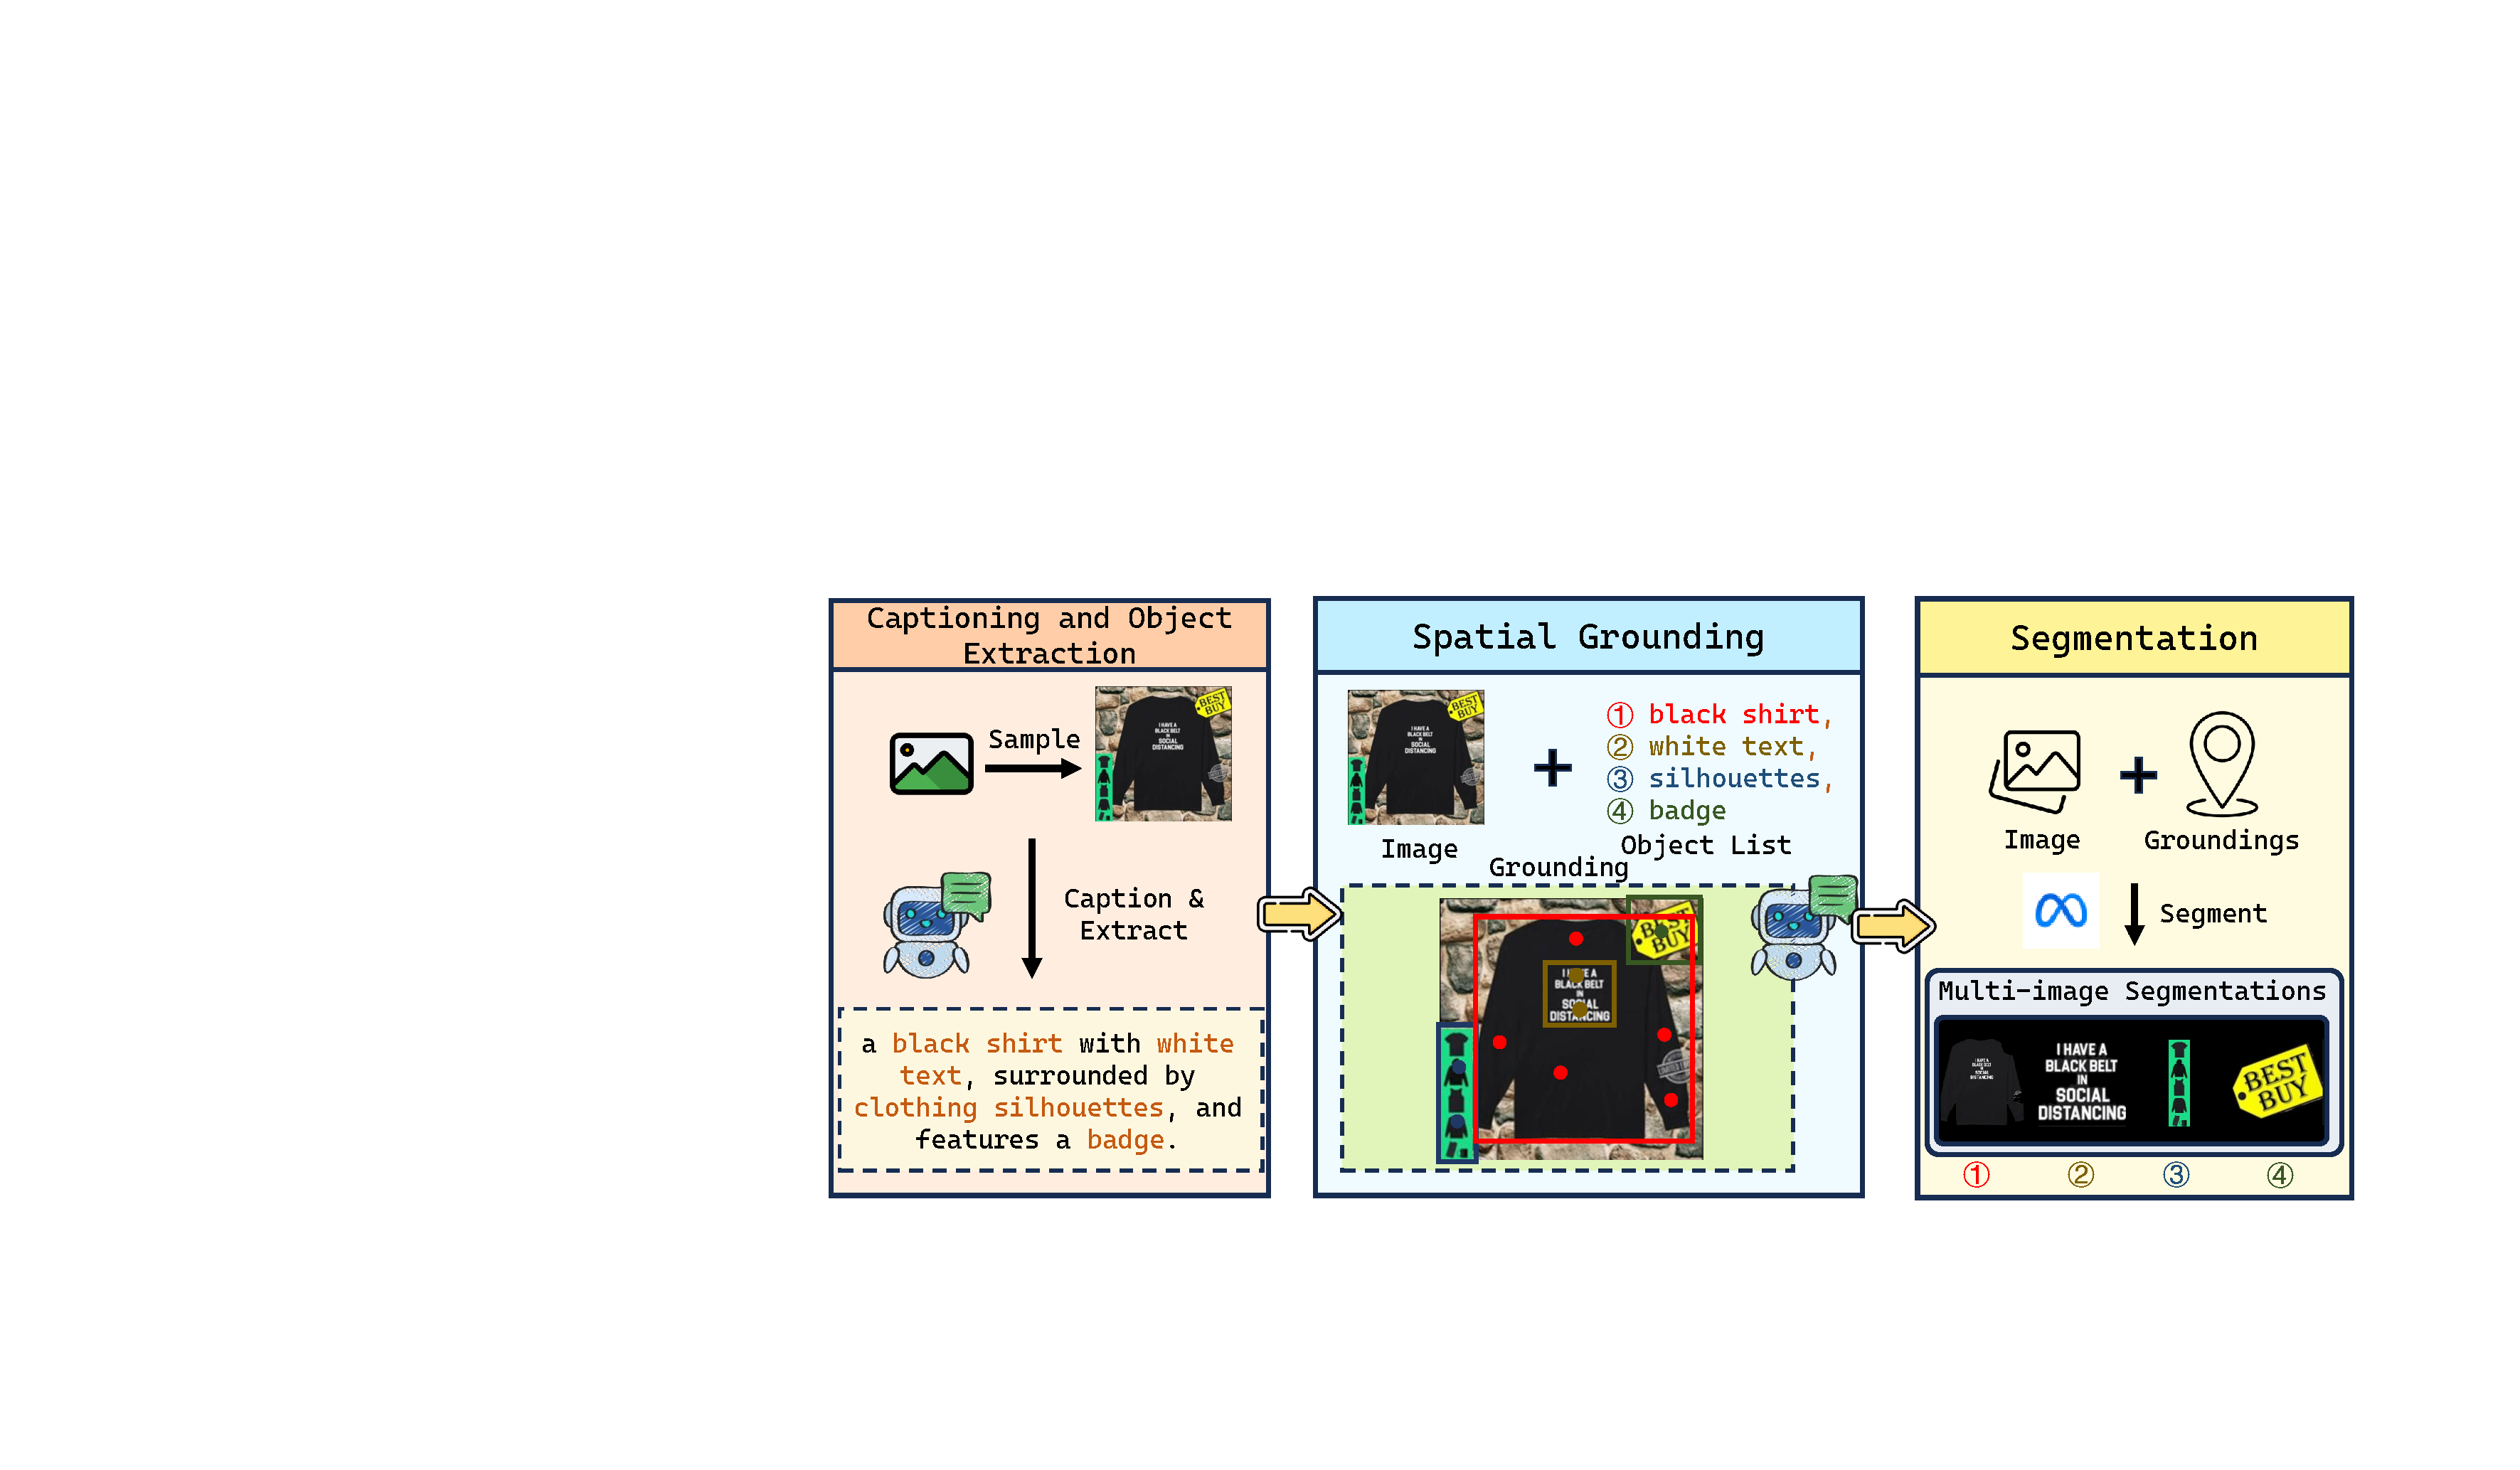
\includegraphics[width=1.0\textwidth]{figures/data_construct.pdf}
\caption{Illustration of the automatic data generation pipeline.}
\label{fig:construction}
\end{figure*}

\paragraph{Data Construction}
To support the large-scale training required for our two-stage paradigm, we developed an automated pipeline for generating high-quality multimodal training data, as shown in Figure~\ref{fig:construction}. This pipeline combines open-source image datasets with state-of-the-art vision-language models (VLMs) and segmentation models, enabling the construction of richly annotated image-text pairs with multiple segmented foreground objects without manual labeling:

\begin{itemize}[left=2pt]
\item \textbf{Captioning and Object Extraction:} A VLM is queried to generate a comprehensive caption describing prominent elements in the image, followed by extracting a list of concrete, distinct, and segmentable objects. This ensures that the generated data focus on tangible visual entities.
\item \textbf{Spatial Grounding:} For each extracted object, the VLM is queried again to identify its spatial location within the image, returning both a tight bounding box and several representative 2D keypoints. These spatial cues constrain the region of interest for subsequent segmentation, improving accuracy and reducing background noise.
\item \textbf{Segmentation:} A segmentation model is employed to extract object masks from the image, guided by the generated bounding boxes and keypoints. This step produces high-quality masks that are both semantically aligned with the object labels and spatially accurate.
\end{itemize}

By applying this automated process to a large corpus of open-source images, we construct a diverse multimodal dataset comprising captioned images annotated with multiple precisely segmented objects. This dataset forms a critical component of our training setup, particularly enabling the object segmentation and image recovery tasks in our training paradigm.


\section{Experiment Details}
\label{sec:Experiment_Details}

\subsection{Benchmark Details}
\label{sec:Benchmark_Details}

\paragraph{DreamBench++}
\label{app:DreamBench_Plus}

\textbf{Data Organization.}
DreamBench++~\citep{peng2025dreambenchpp} comprises 150 high-quality reference images, sourced from Unsplash, Rawpixel, and Google Images, encompassing a balanced mix of subjects. These are evenly divided into three broad categories: \textit{objects}, \textit{living subjects} (humans and animals), and \textit{styles} (illustrative, painterly, etc.), ensuring visual and conceptual diversity.

In total, DreamBench++ offers \textbf{1,350 prompts} ($150 \times 9$), representing a substantial scale-up over the original DreamBench (30 subjects $\times$ 25 prompts). Relative to DreamBench, the dataset is \textbf{5$\times$ larger in subjects} and \textbf{54$\times$ larger in prompts}, enabling broader evaluation of generative performance.

\textbf{Evaluation Metric.}
DreamBench++ adopts an automatic, GPT-4o-based evaluation protocol designed to closely mirror human judgment. Each generated image is assessed against both its reference image and its corresponding prompt, using two complementary axes:

\begin{itemize}[left=2pt, itemsep=0.5pt,topsep=0.5pt]
\item \textbf{Concept Preservation (CP):} Measures fidelity between the generated image and the reference. Key attributes include shape, color, texture, and facial details.
\item \textbf{Prompt Following (PF):} Evaluates how well the generation aligns with the prompt in terms of relevance, accuracy, completeness, and contextual appropriateness.
\end{itemize}

Each axis is scored on a \textbf{five-level ordinal scale} from 0 (Very Poor) to 4 (Excellent), avoiding the complexity and bias of pairwise comparisons.

\paragraph{DreamBench}
The original DreamBench~\citep{ruiz2023dreamboothfinetuningtexttoimage} dataset consists of 30 subjects, each paired with 25 prompts, totaling 750 prompt-image pairs. It serves as a foundational benchmark for evaluating personalized image generation models, focusing on the model's ability to maintain subject identity across diverse prompts.


\subsection{Baselines}
\label{sec:Baselines_Details}

We compare our method against various baselines, categorized as follows:

\begin{itemize}[left=2pt, itemsep=0.5pt,topsep=0.5pt]
\item \textbf{Textual Inversion}~\citep{gal2022imageworthwordpersonalizing} learns a new word embedding to represent a specific concept, enabling personalized image generation by incorporating the new token into prompts. It requires a few images of the subject and fine-tunes the embedding without altering the base model weights.
\item \textbf{DreamBooth}~\citep{ruiz2023dreamboothfinetuningtexttoimage}: DreamBooth fine-tunes a pre-trained text-to-image model to bind a unique identifier with the subject's visual concept, allowing for personalized generation. It requires several images of subject and modifies model weights to capture subject-specific details.

\item \textbf{BLIP-Diffusion}~\citep{li2023blipdiffusionpretrainedsubjectrepresentation}: This approach introduces a pre-trained multimodal encoder to provide subject representations for the diffusion generator, enabling controllable multimodal image generation. 

\item \textbf{KOSMOS-G}~\citep{Kosmos-G}: KOSMOS-G is a multimodal large language model designed for zero-shot image generation from interleaved vision-language inputs, including multiple images and text. It aligns the output space of a transformer-based causal language model with a diffusion-based image decoder using a lightweight AlignerNet and compositional instruction tuning. This architecture enables KOSMOS-G to perceive complex multimodal prompts and generate coherent, subject-driven images without modifying the base image decoder.

\item \textbf{Emu2}~\citep{emu2}: Emu2 is a 37-billion-parameter generative multimodal model trained on large-scale multimodal sequences with a unified autoregressive objective. It exhibits strong in-context learning abilities for various multimodal tasks, including visual prompting and object-grounded generation.

\item \textbf{IP-Adapter}~\citep{ye2023ip-adapter}: IP-Adapter is a lightweight adapter that enables image prompt capability for pre-trained text-to-image diffusion models. It integrates image features into the generation process without modifying the base model, supporting flexible and efficient image-to-image generation.

\item \textbf{DreamEngine}~\citep{dreamengine}: DreamEngine is a unified framework that integrates multimodal encoders with diffusion models through a two-stage training approach, enabling advanced text-image interleaved control and achieving state-of-the-art performance in generating images with complex, concept-merged inputs.

\item \textbf{Unified-IO 2}~\citep{lu2023unifiedio2}: Unified-IO 2 is an autoregressive multimodal model capable of understanding and generating images, text, audio, and actions. It tokenizes various modalities into a shared semantic space and processes them with a single encoder-decoder transformer. Trained from scratch on a large multimodal pre-training corpus and fine-tuned on an ensemble of 120 datasets, Unified-IO 2 achieves state-of-the-art performance on the GRIT benchmark and strong results across more than 35 benchmarks. 

\item \textbf{Lumina-mGPT}~\citep{2024lumina}: Lumina-mGPT is a multimodal autoregressive models designed for flexible photorealistic text-to-image generation. It employs a pretrained decoder-only transformer as a unified framework for modeling multimodal token sequences. Through multimodal Generative PreTraining (mGPT) and subsequent Flexible Progressive Supervised Finetuning (FP-SFT) and Omnipotent Supervised Finetuning (Omni-SFT), Lumina-mGPT demonstrates versatile multimodal capabilities, including visual generation tasks, controllable generation tasks and vision-language tasks. 

\end{itemize}



\section{Qualitative Study}
\label{sec:Qualitative_Study}

\subsection{Image Reconstruction}
\label{sec:Reconstruction}

\begin{figure*}[t]
\centering
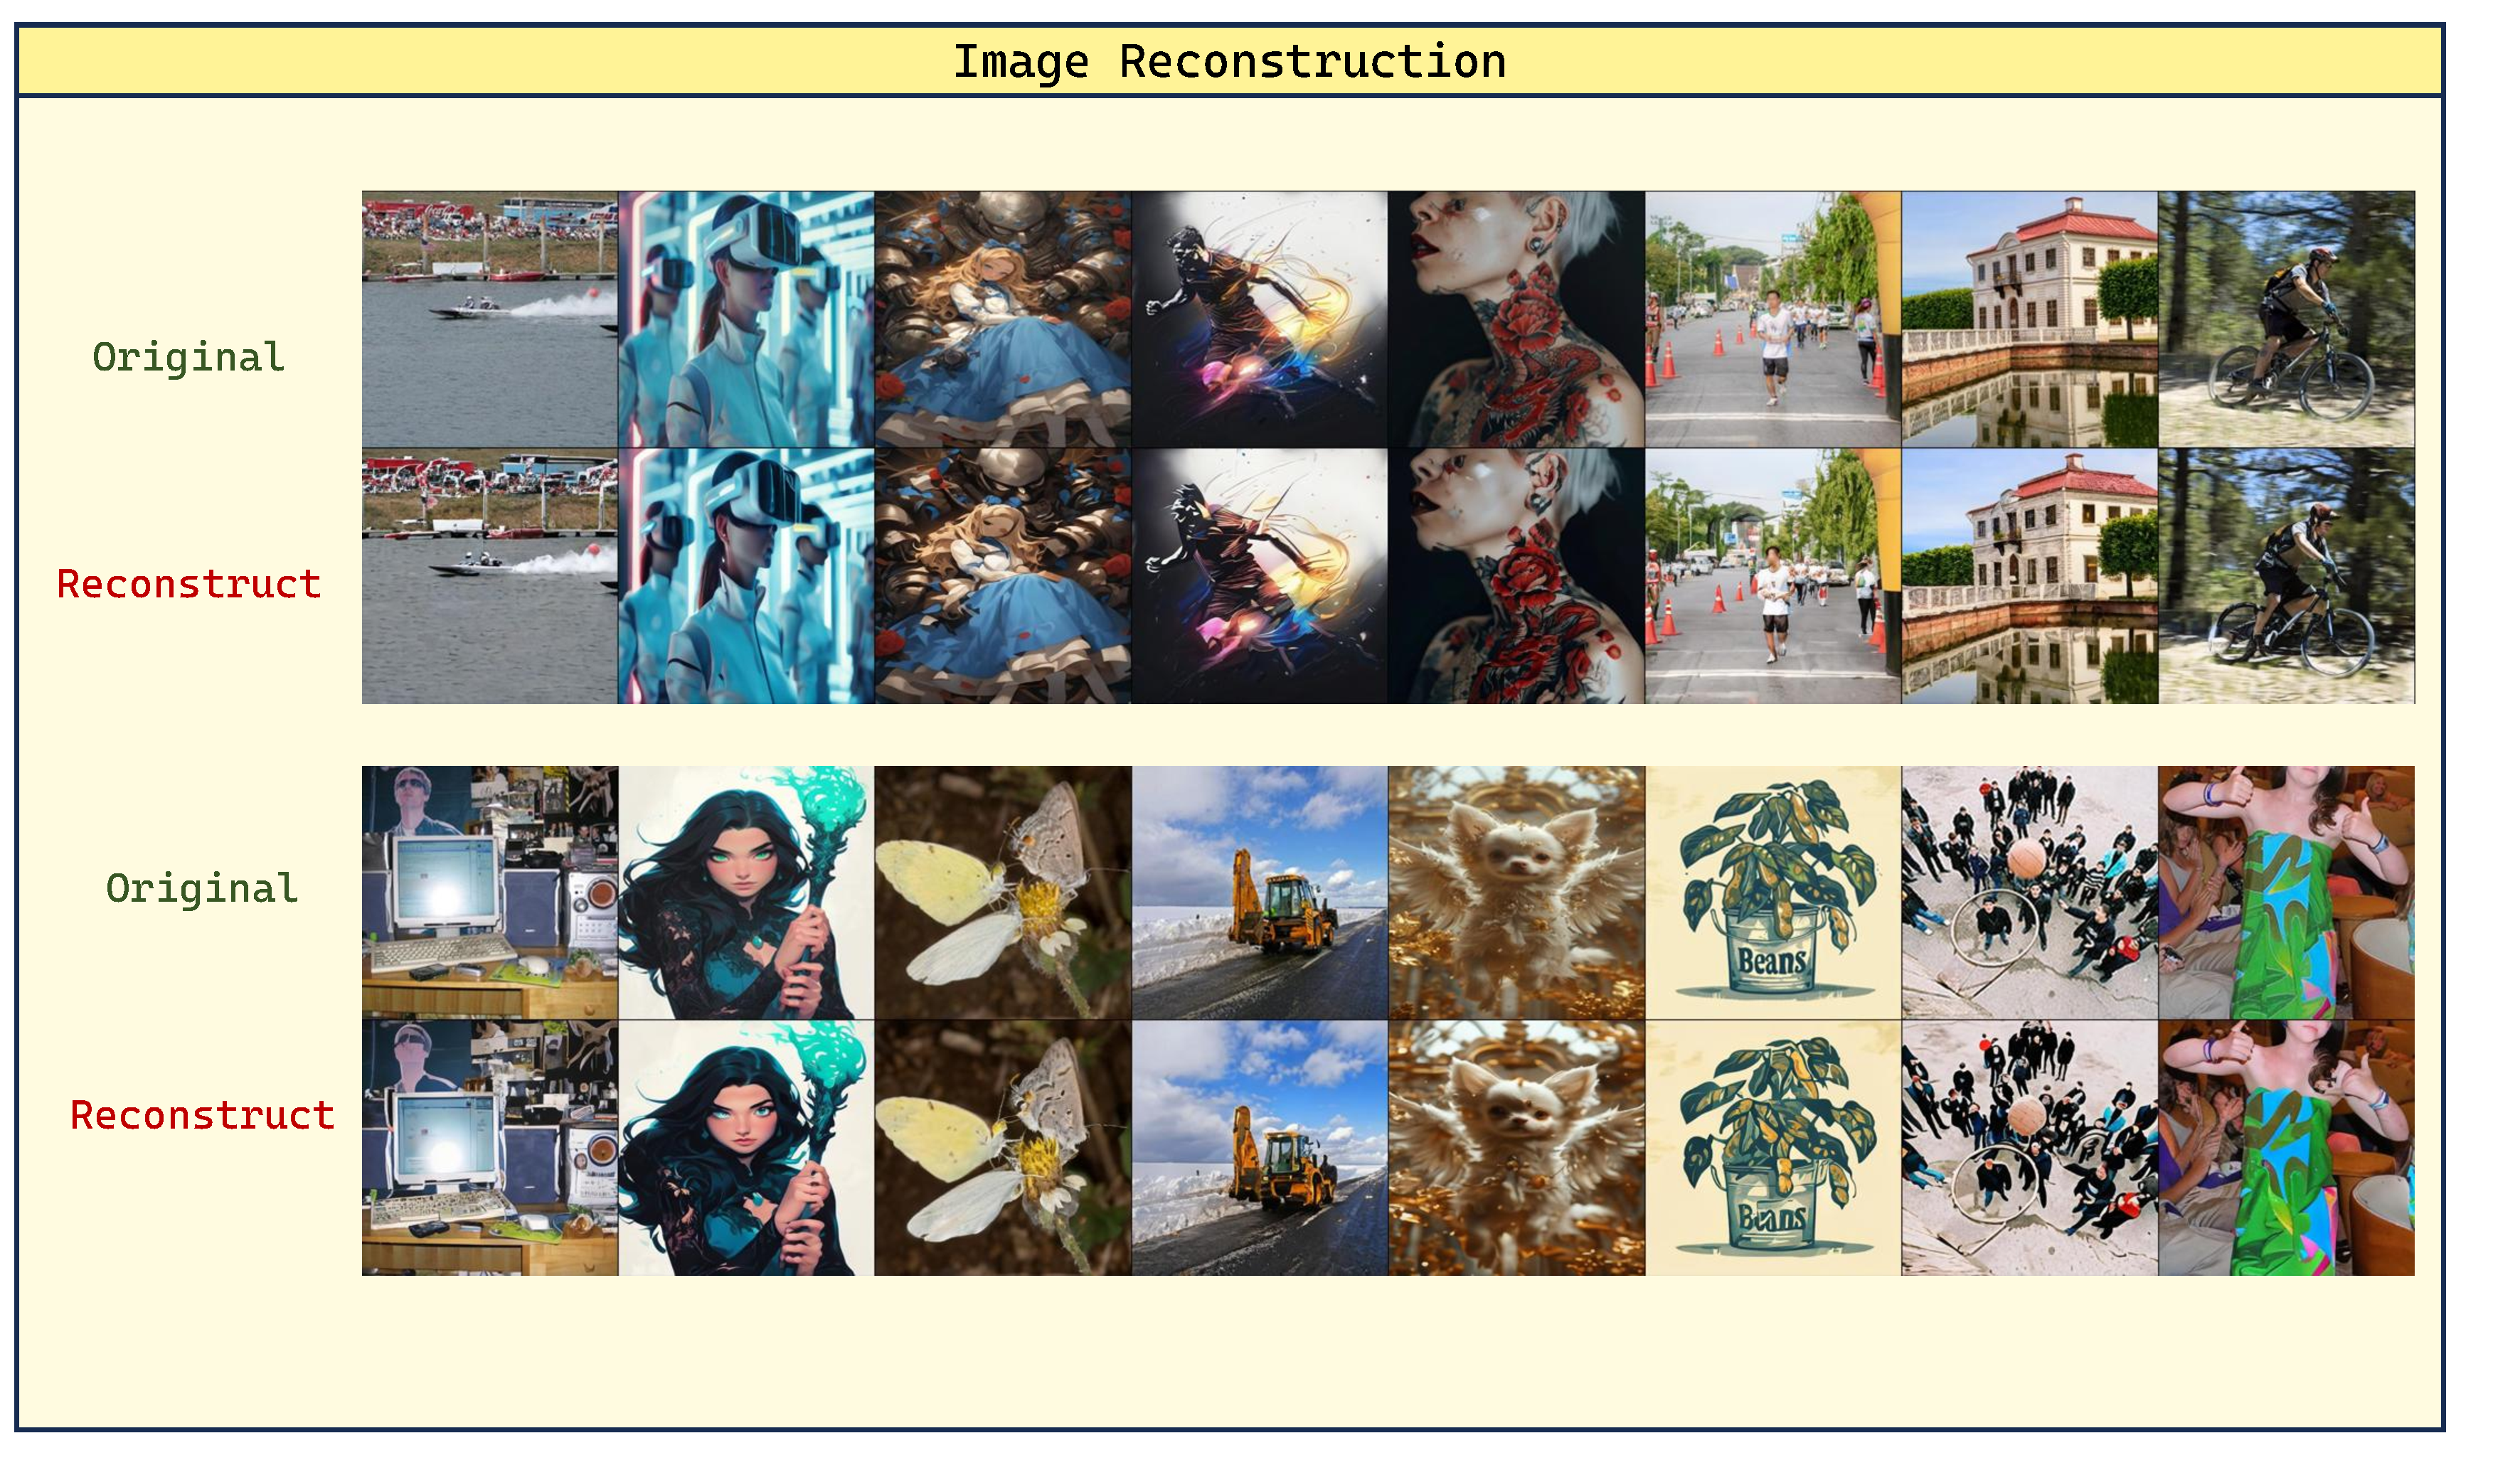
\includegraphics[width=0.85\textwidth]{figures/reconstrucion.pdf}
\caption{Qualitative comparison of image reconstruction results using \model.}
\label{fig:reconstruction}
\end{figure*}

\begin{figure*}[t]
\centering
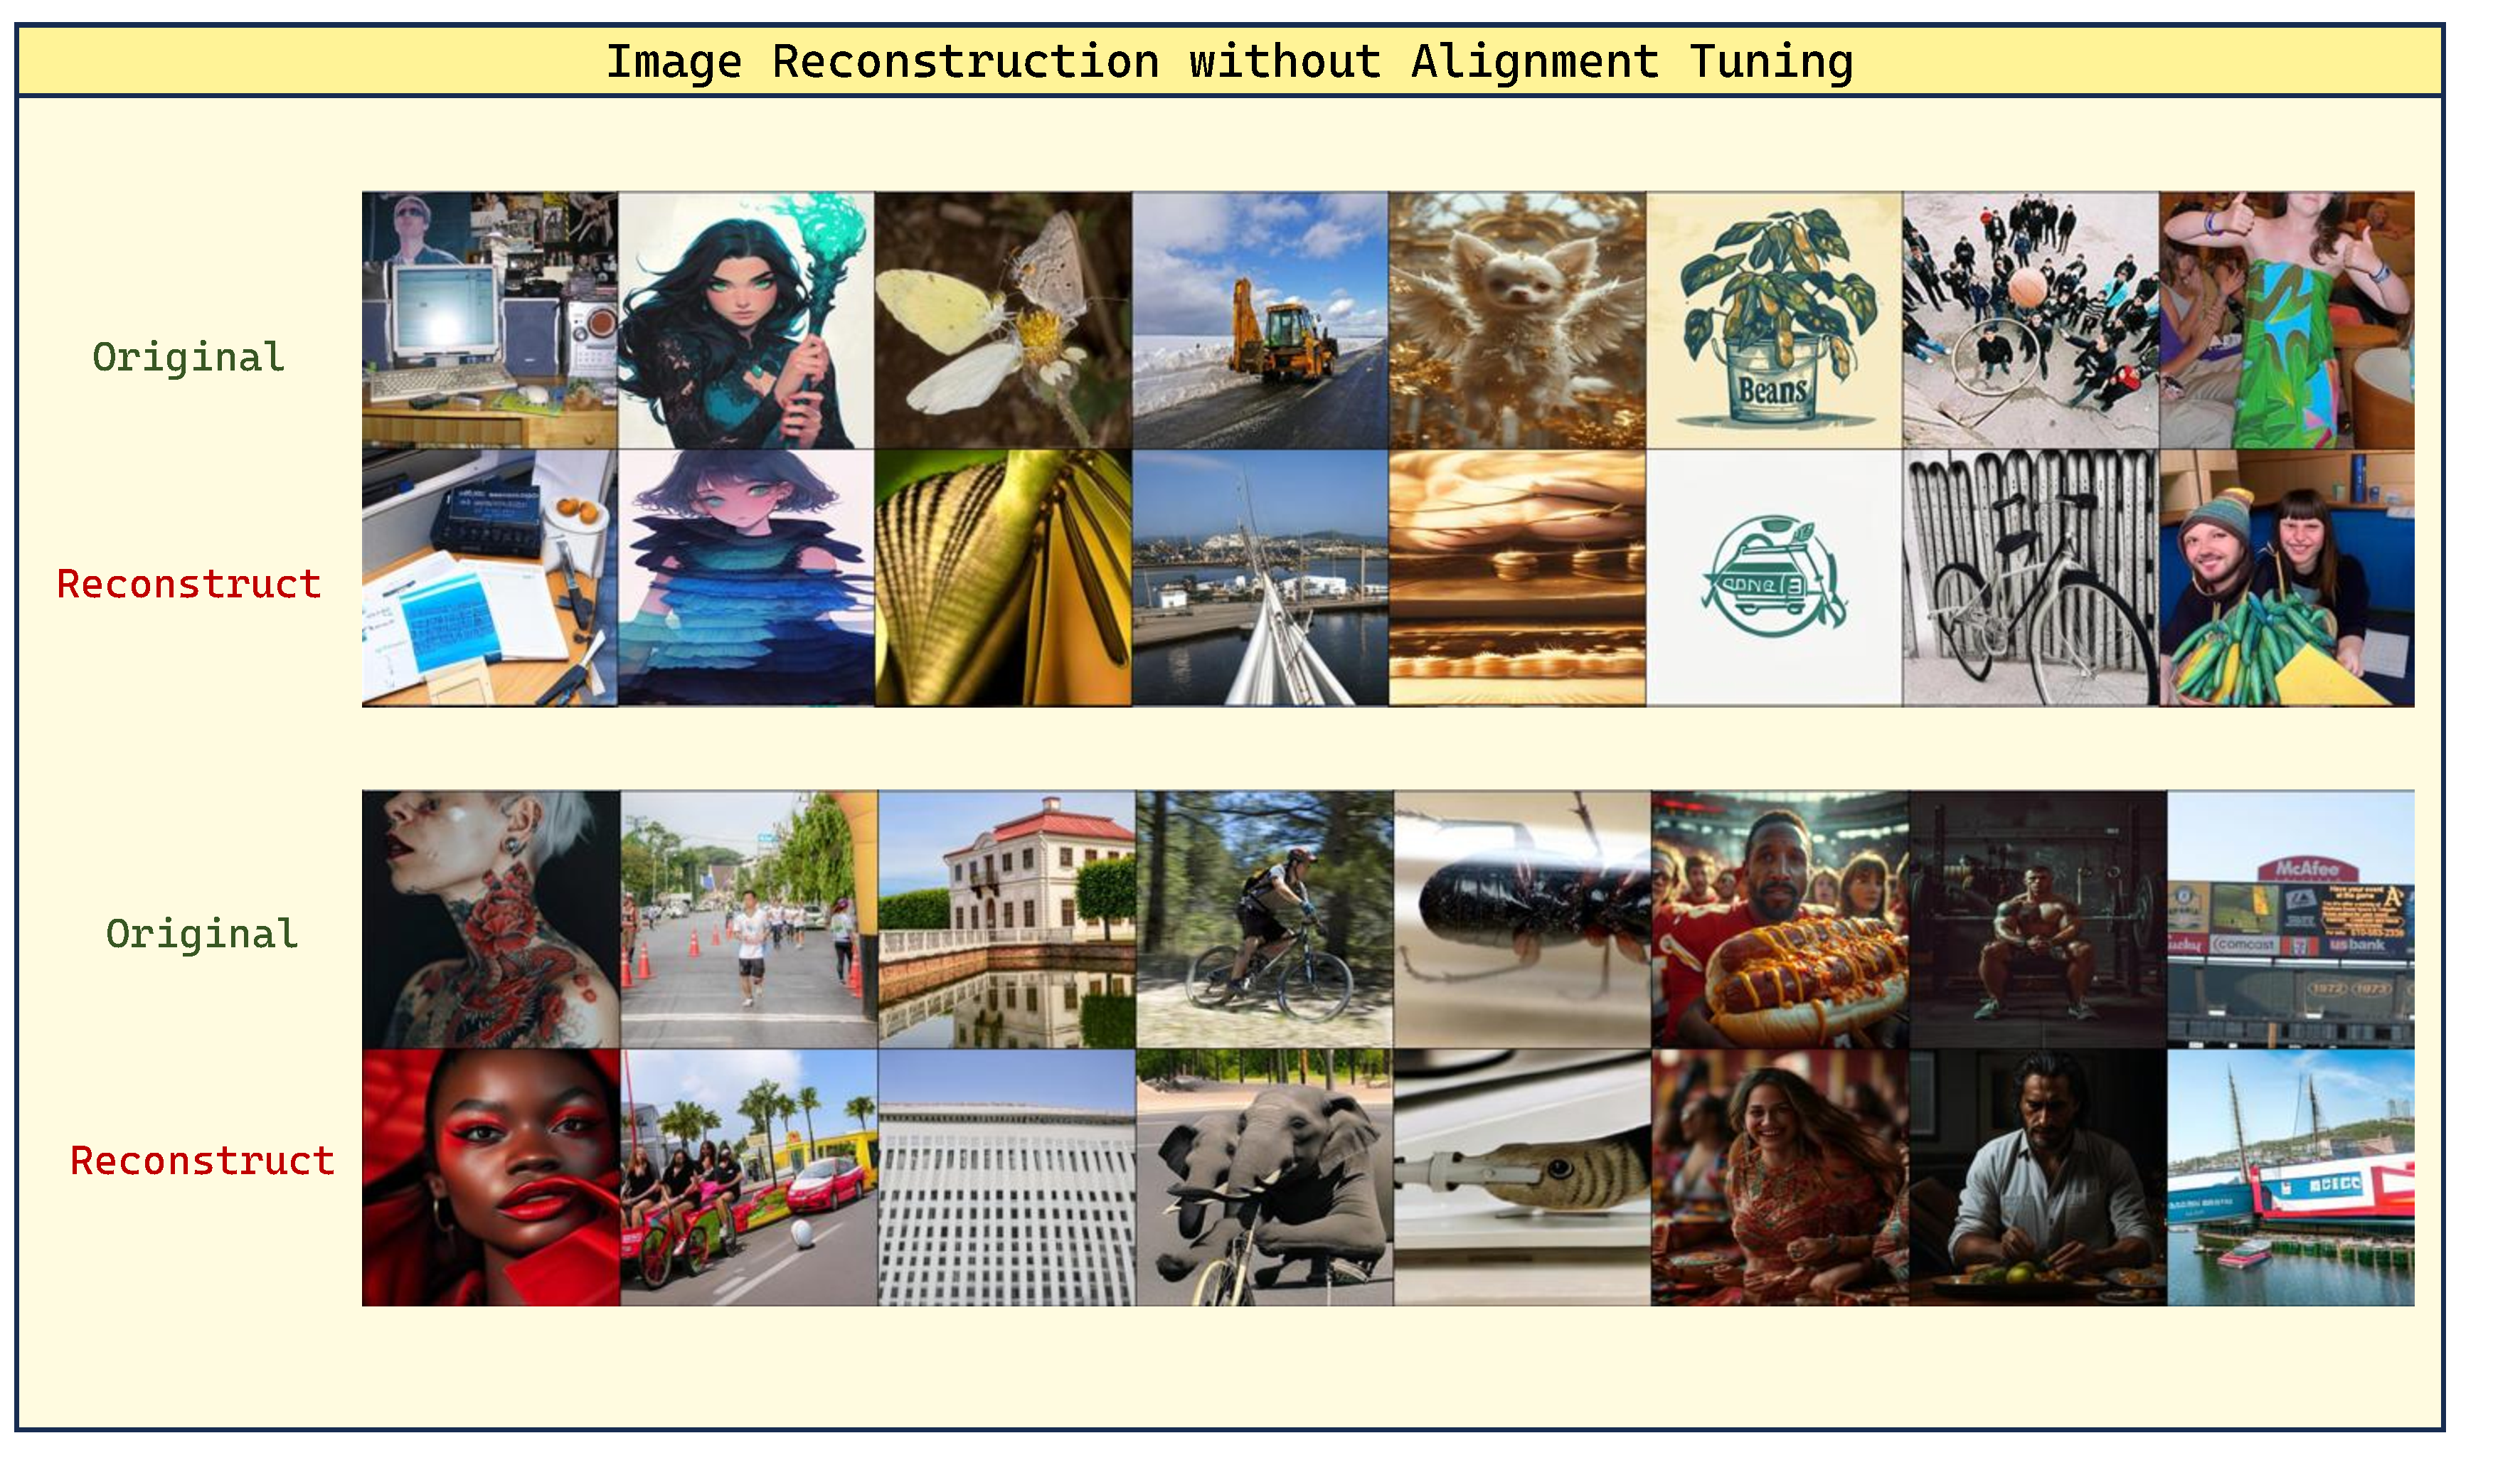
\includegraphics[width=0.85\textwidth]{figures/reconstrucion_wo_alignment.pdf}
\caption{Image reconstruction results of \model \textit{without} alignment tuning.}
\label{fig:reconstruction_wo_align}
\end{figure*}

As illustrated in Figures~\ref{fig:reconstruction} and \ref{fig:reconstruction_wo_align}, \model demonstrates strong image reconstruction capabilities following two-stage training. Notably, it is able to effectively reconstruct input images and preserve fine-grained visual details, even when input images are of low resolution (224×224) and outputs are generated at 512×512 resolution.

In contrast, when alignment tuning is omitted, although the model benefits from the pretrained multimodal encoder and the proposed architecture, it tends to treat the input image as a visual prompt akin to a caption. As shown in Figure~\ref{fig:reconstruction_wo_align}, this leads to outputs that resemble descriptive interpretations of the input rather than faithful reconstructions. Consequently, visual fidelity and spatial consistency degrade significantly without alignment tuning.

\subsection{Text-guided Image Segmentation}
\label{sec:Segmentation}


\begin{figure*}[t]
\centering
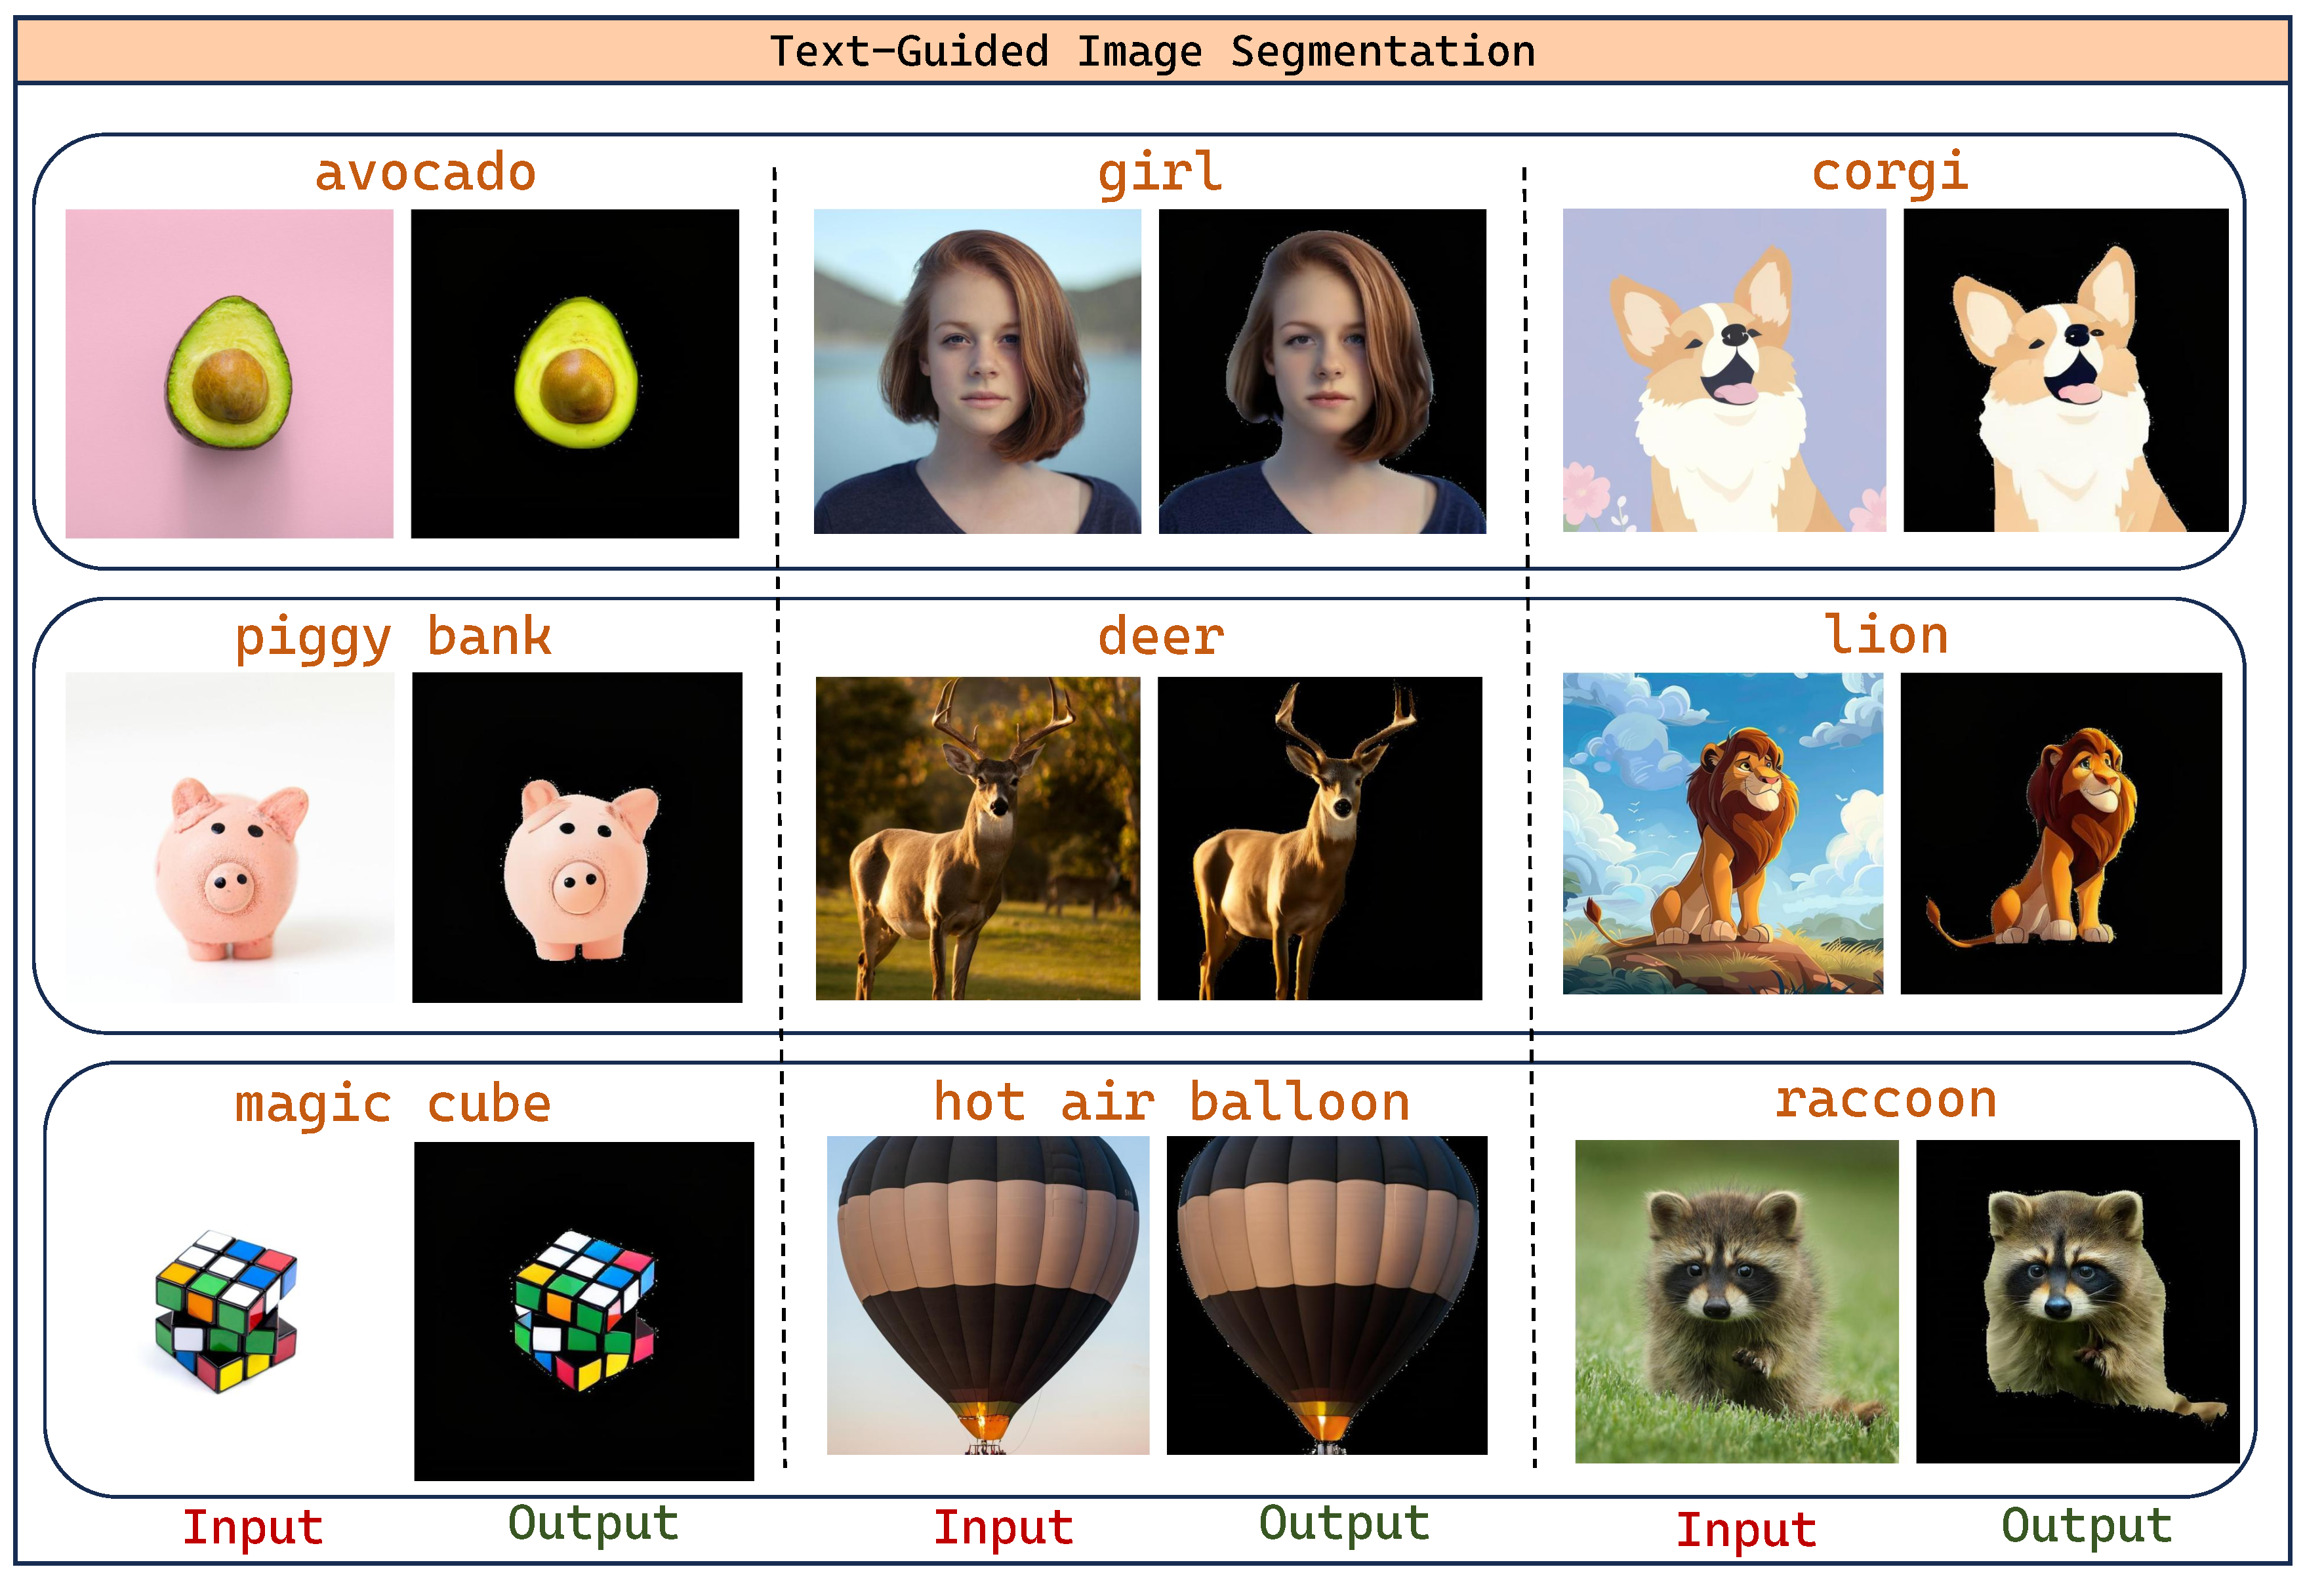
\includegraphics[width=1.0\textwidth]{figures/segmentation_example.pdf}
\caption{Qualitative results of text-guided image segmentation using \model.}
\label{fig:segmentation_example}
\end{figure*}

We evaluate \model on the DreamBench\texttt{++} benchmark to assess its performance in text-guided image segmentation. As demonstrated in Figure~\ref{fig:segmentation_example}, \model successfully identifies and segments visual concepts corresponding to the given textual prompts. These results highlight the model's ability to generalize across tasks and showcase its robust multimodal understanding and generation.

\subsection{Multi-Image Generation}
\label{sec:Multi-Image}

\begin{figure*}[t]
\centering
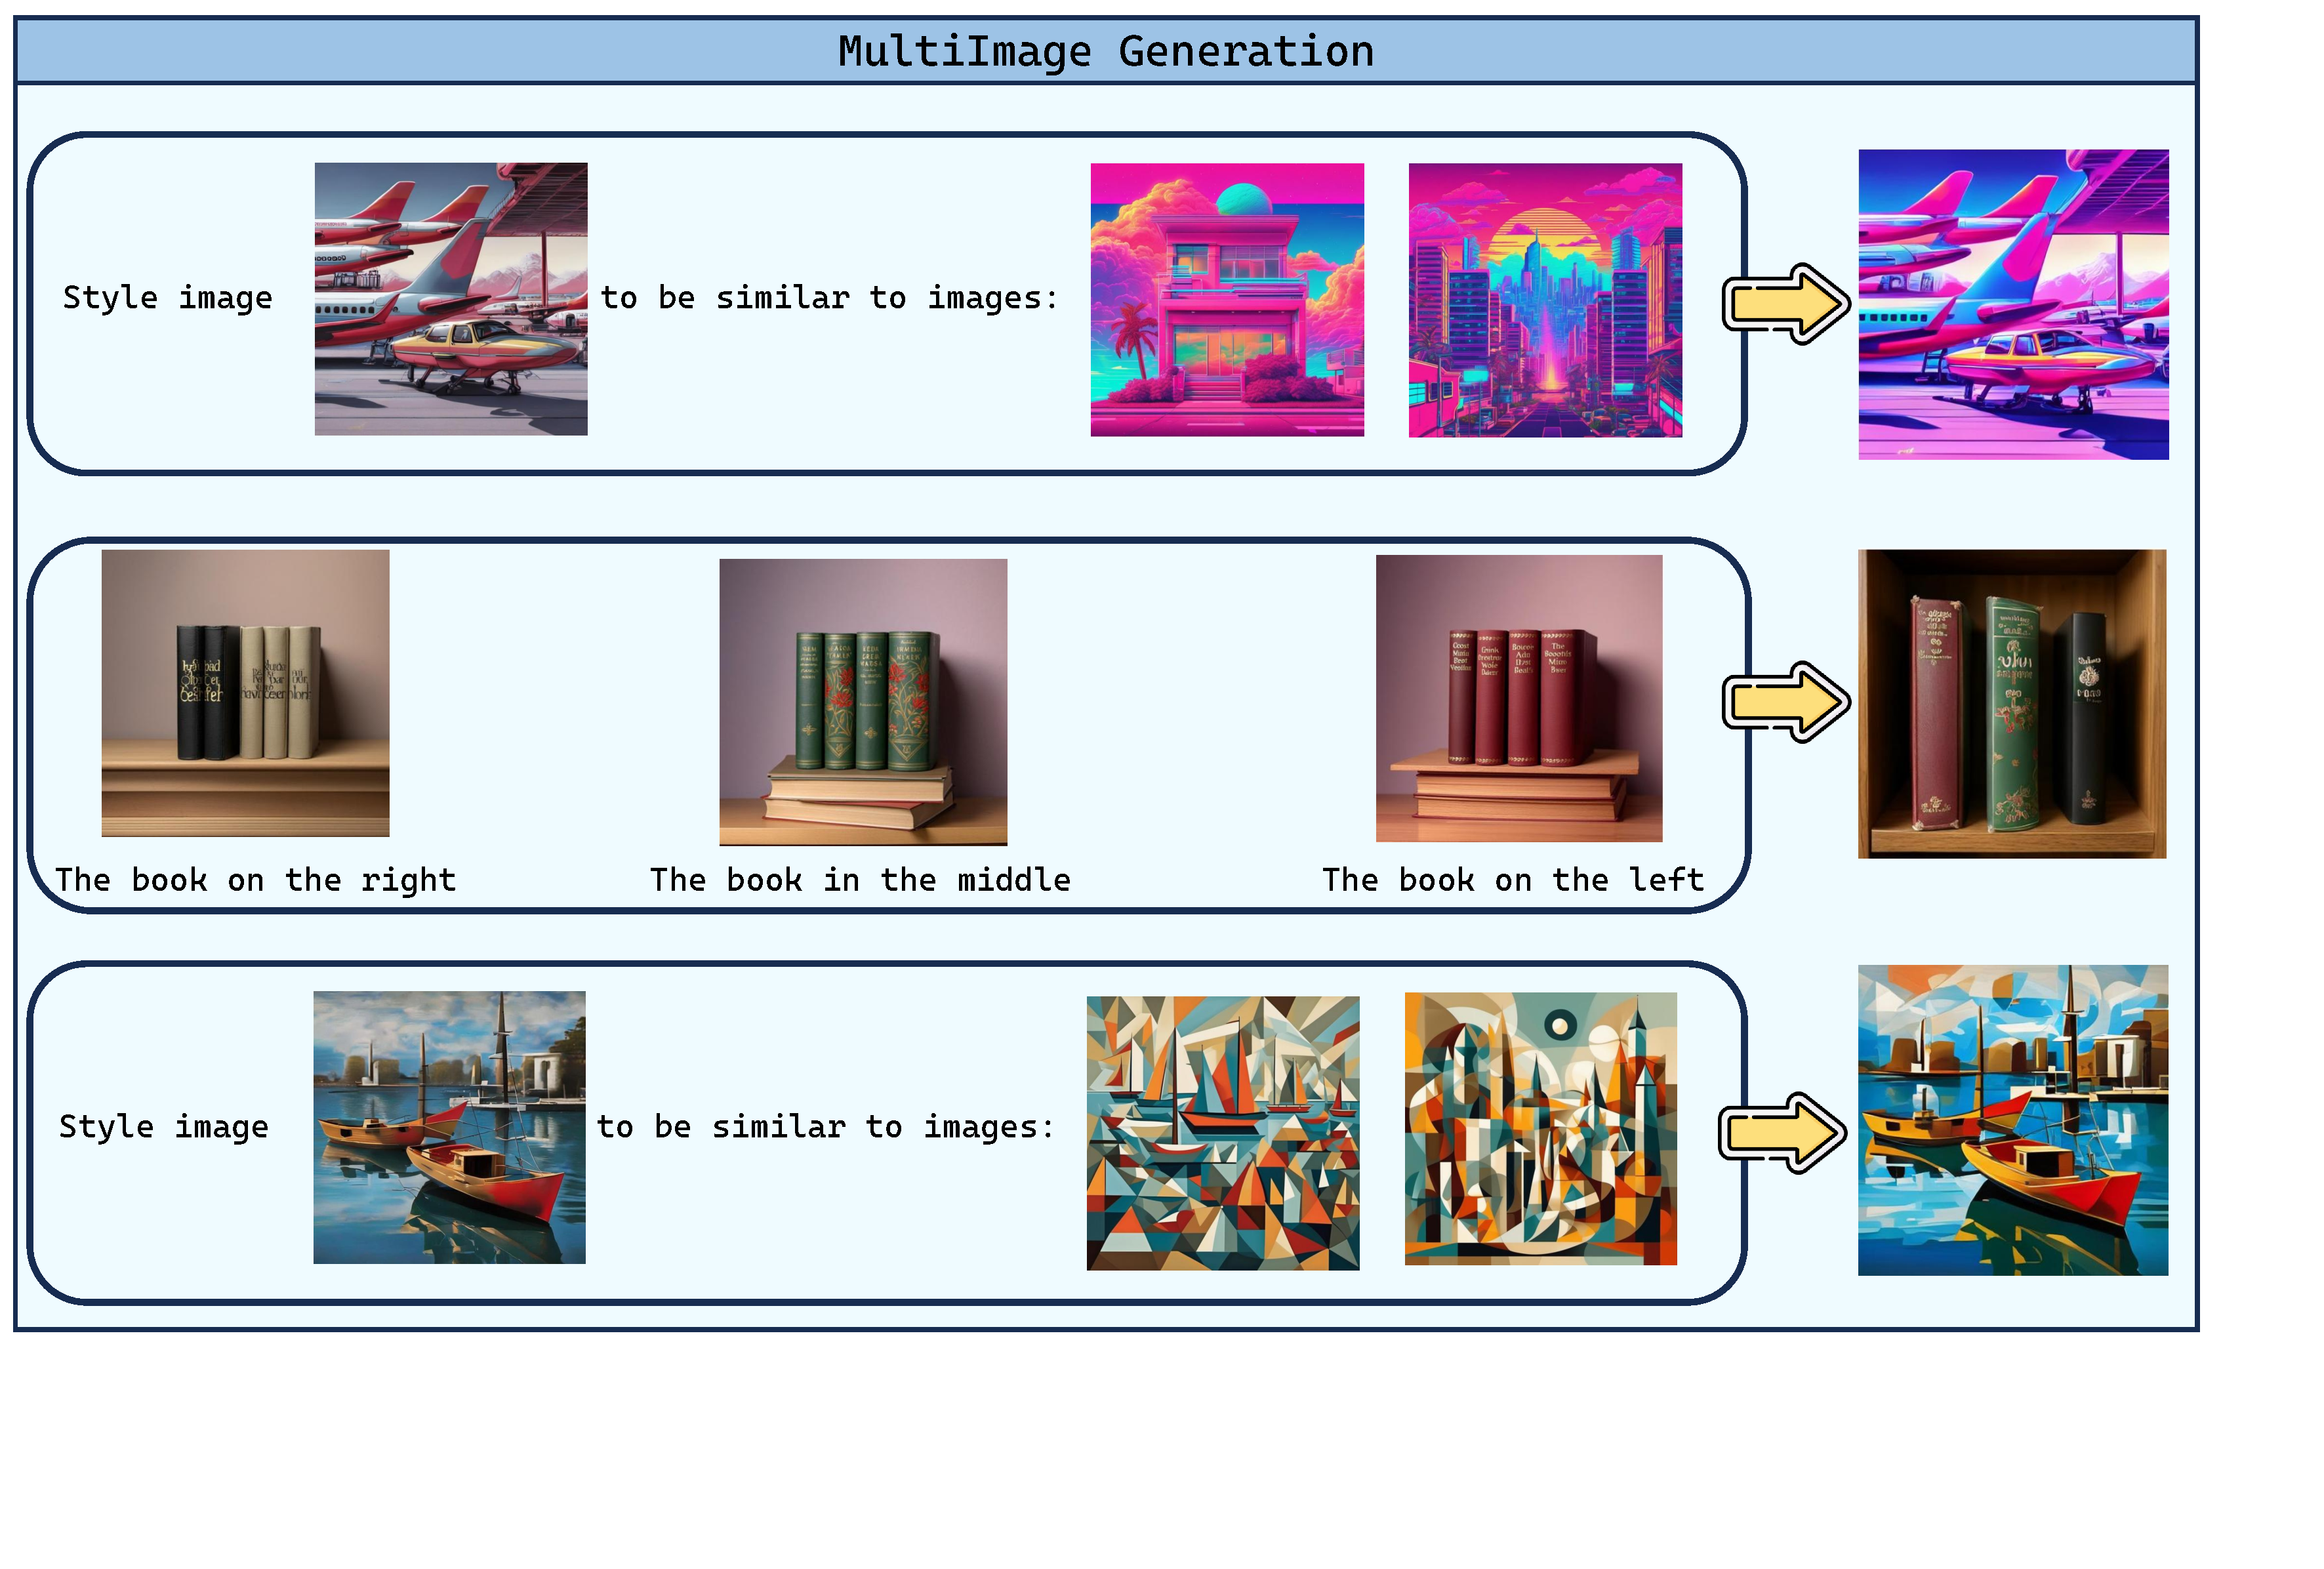
\includegraphics[width=0.85\textwidth]{figures/multi_img.pdf}
\caption{Qualitative results for multi-image generation.}
\label{fig:multi_image}
\end{figure*}

We evaluate \model on multi-image generation tasks using the X2I dataset~\citep{OmniGen}. As shown in Figure~\ref{fig:multi_image}, the model is capable of generating visually consistent outputs conditioned the multi-image inputs. The generated images reflect coherent semantics, style, and layout across the samples.

\subsection{Multimodal In-Context Image Generation}
\label{sec:mmicl}

\begin{figure*}[t]
\centering
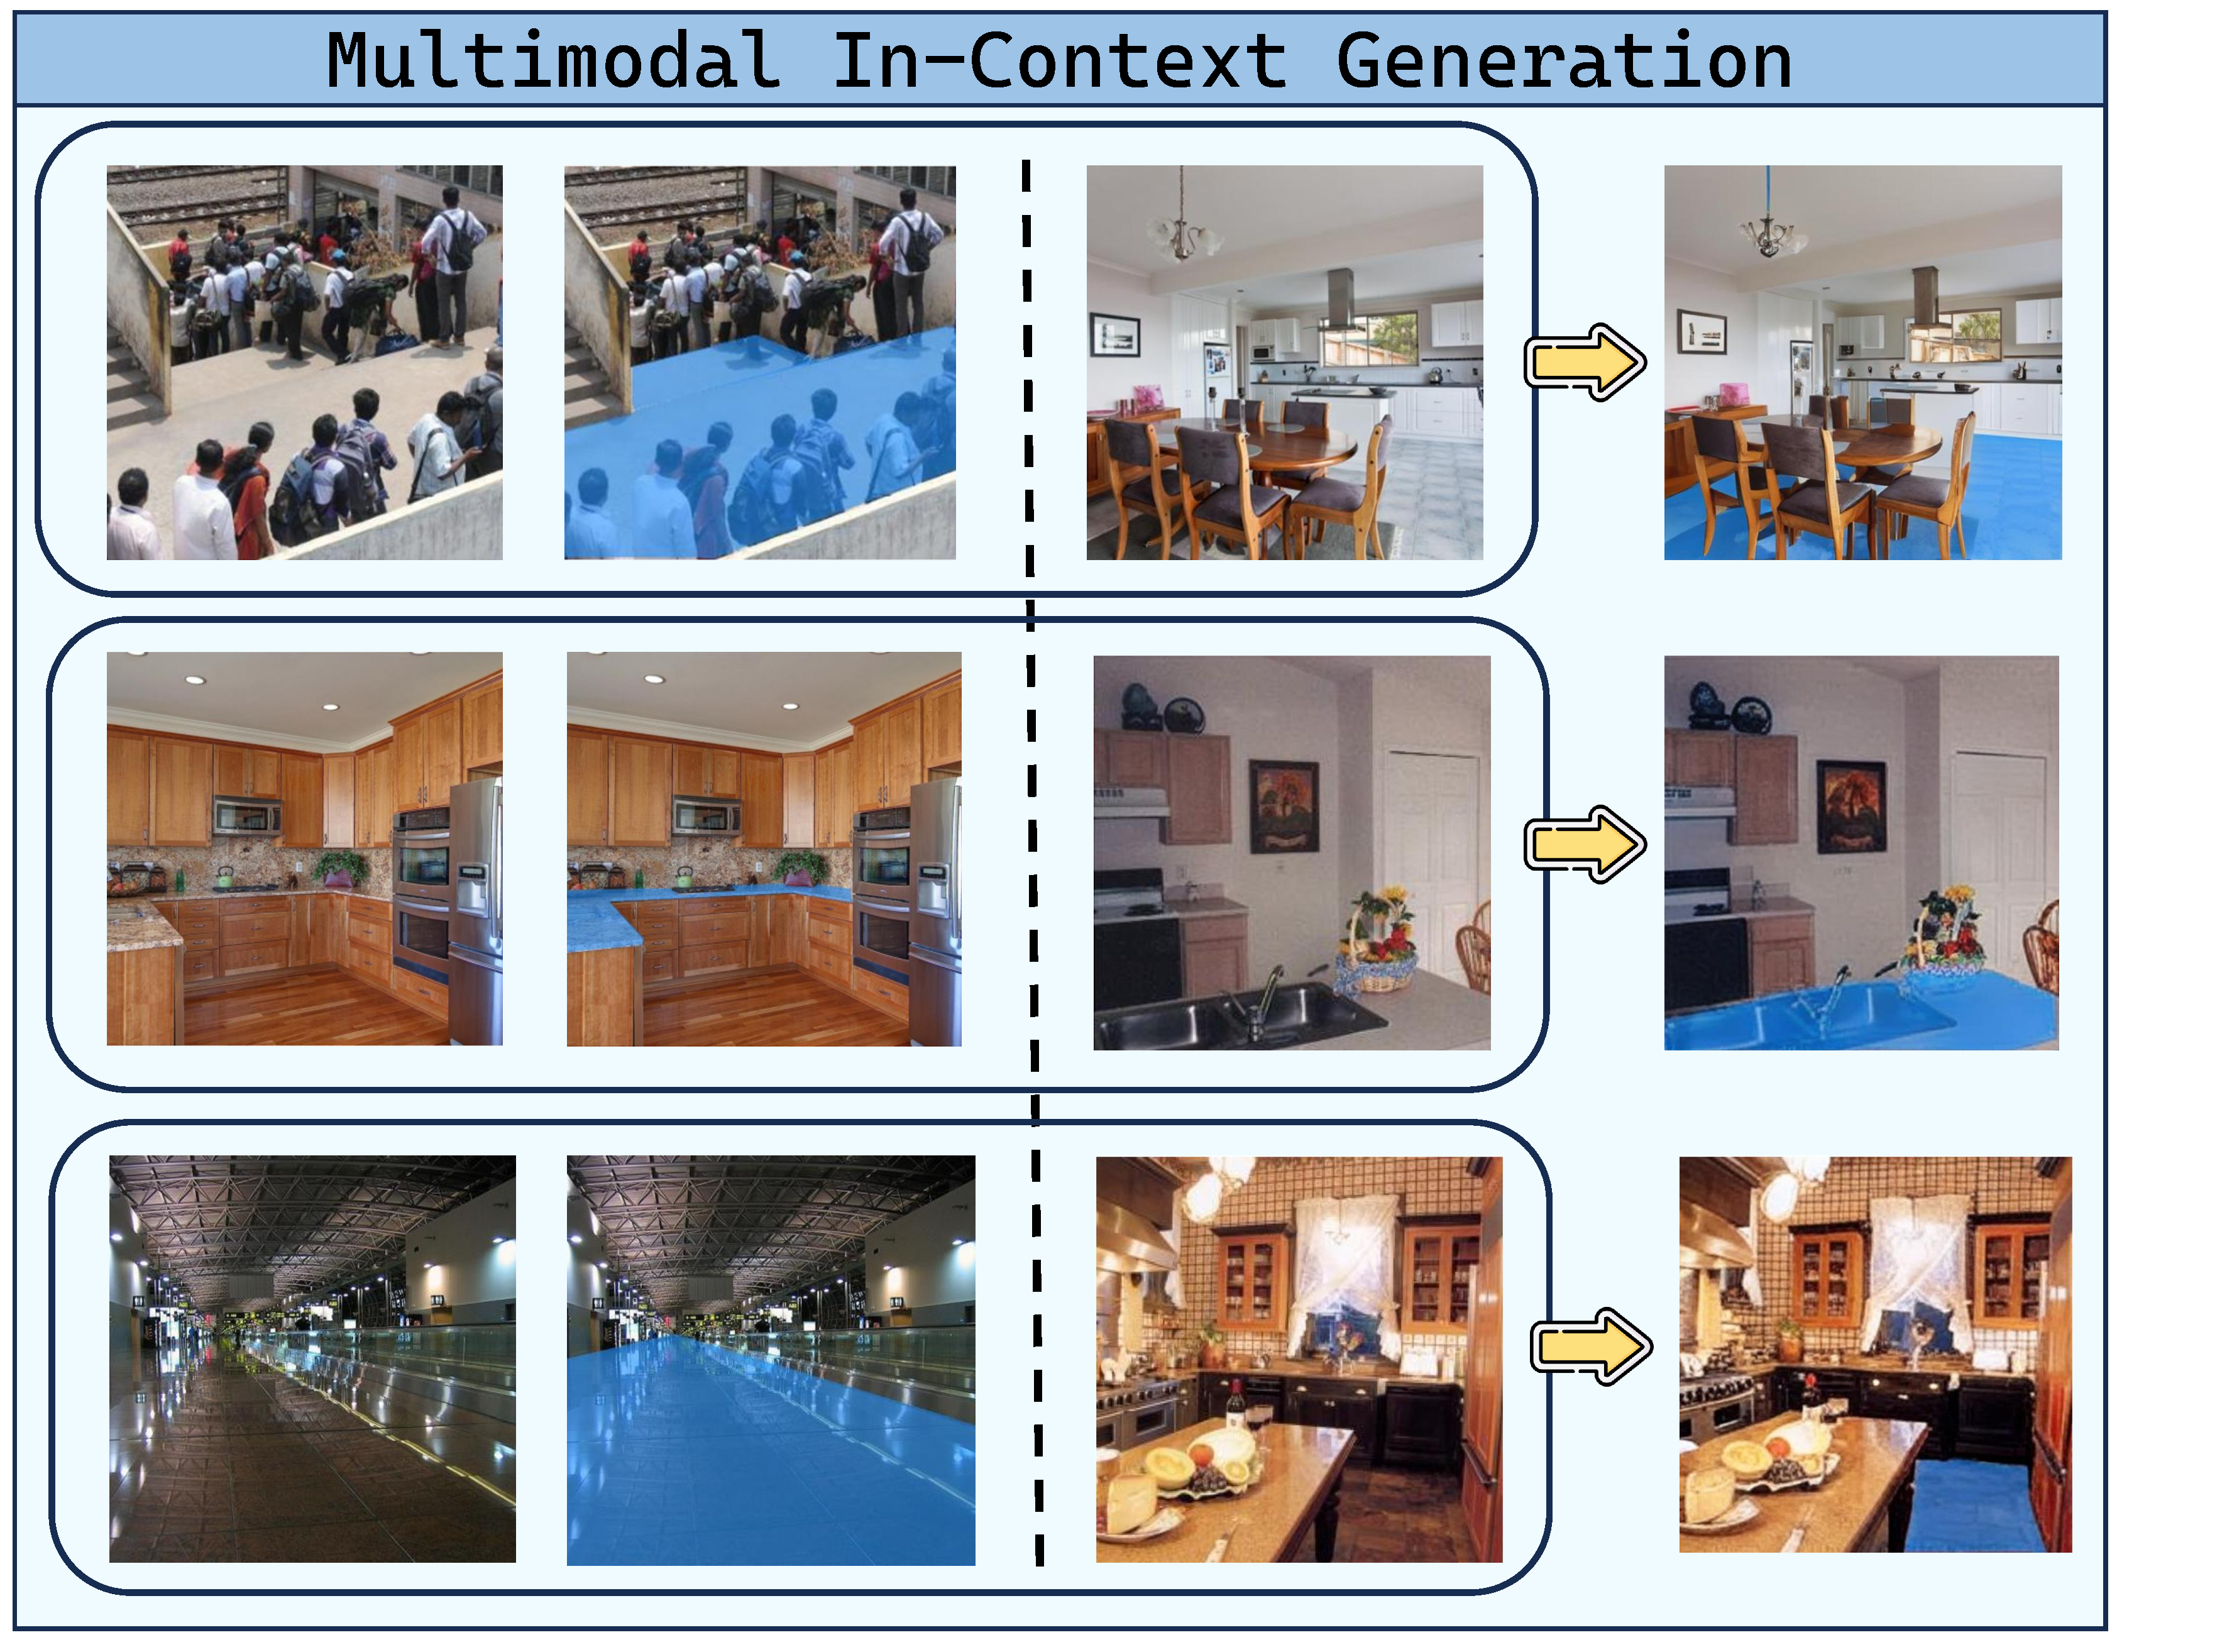
\includegraphics[width=0.75\textwidth]{figures/icl_exp.pdf}
\caption{Qualitative examples from multimodal in-context image generation. The model adapts to patterns in the visual context.}
\label{fig:icl_example}
\end{figure*}

To assess \model's few-shot generalization capabilities, we evaluate it on the multimodal in-context image generation task using the X2I-ICL dataset~\citep{OmniGen}. As illustrated in Figure~\ref{fig:icl_example}, \model learns to synthesize images that follow the stylistic patterns demonstrated in the in-context examples. This indicates its capability to infer complex visual trends and align generation with image context.

\section{Versatility Across Different Multimodal Tasks}
\label{app:applications}

To assess the broad applicability of our proposed framework, we evaluate \model across a diverse set of multimodal generation tasks, including text-guided image segmentation, subject-driven image generation, multi-image generation, and multimodal in-context learning. For each task, we apply supervised fine-tuning where necessary, ensuring robust generalization while maintaining architectural consistency.

\paragraph{Image Segmentation.}
We evaluate this task directly after Stage 1 training, without additional fine-tuning. The model demonstrates strong object localization and mask precision from prompt-aligned inputs, confirming the effectiveness of the proposed training pipeline and segmentation-aware data construction process.

\paragraph{Subject-driven Image Generation.}
This task is evaluated using the model at the end of Stage 2. No additional task-specific tuning is applied. The model successfully generates high-fidelity, identity-preserving images consistent with subject descriptors.

\paragraph{Multi-Image Generation.}
We fine-tune the Stage 2 model on a subset of X2I-subject-driven~\citep{OmniGen} dataset for two additional epochs using a reduced learning rate of $5 \times 10^{-5}$. All other optimization settings remain consistent with Stage 2. The dataset is split into disjoint training and test sets, and quantitative results are reported on the test split. The model learns to generate visually diverse yet semantically aligned images for the same input.

\paragraph{Multimodal In-Context Learning.}
We fine-tune the model for 10 epochs on the X2I-ICL dataset~\citep{OmniGen}, which features sequences of input-output pairs for in-context generalization. We use a learning rate of $5 \times 10^{-5}$ and ensure a strict train-test separation. The model adapts to context examples and generates new samples following the observed patterns, showing strong in-context learning performance without explicit prompting engineering.

\paragraph{Conclusion.}
The qualitative results presented in Section~\ref{sec:Qualitative_Study} confirm the versatility of \model across a wide range of tasks. Notably, the model adapts to each task without architectural modifications, requiring only lightweight fine-tuning.

\section{Limitations}
\label{app:limitation}

Our work presents a promising alternative to diffusion-based methods for multimodal-conditioned image generation. As such, our focus is on evaluating performance under comparable conditions—i.e., with similar model capacities and training paradigms.
However, the effectiveness of our approach is currently constrained by the limitations of available autoregressive (AR) backbone models. Due to the lack of high-performance AR generators, \model exhibits shortcomings in several aspects of image generation, including spatial reasoning, object counting, fine-grained human rendering, and stylization. These limitations reflect the current gap between current SOTA diffusion and autoregressive architectures in terms of generation fidelity and domain generalization.
Additionally, while our training data is sourced from publicly available datasets and our synthetic data pipeline includes NSFW safeguards, a comprehensive evaluation of safety, fairness, and potential misuse remains lacking. Future work should incorporate thorough assessments of model biases and unintended behaviors.
Finally, while our framework demonstrates strong versatility across diverse multimodal tasks, achieving competitive performance in specific domains may require more specialized training and the integration of more powerful multimodal encoders and generators. These initial findings nonetheless highlight the framework's potential as a unified and efficient foundation for conditional multimodal image generation.


% 
\newpage
\section*{NeurIPS Paper Checklist}

%%% BEGIN INSTRUCTIONS %%%
The checklist is designed to encourage best practices for responsible machine learning research, addressing issues of reproducibility, transparency, research ethics, and societal impact. Do not remove the checklist: {\bf The papers not including the checklist will be desk rejected.} The checklist should follow the references and follow the (optional) supplemental material.  The checklist does NOT count towards the page
limit. 

Please read the checklist guidelines carefully for information on how to answer these questions. For each question in the checklist:
\begin{itemize}
    \item You should answer \answerYes{}, \answerNo{}, or \answerNA{}.
    \item \answerNA{} means either that the question is Not Applicable for that particular paper or the relevant information is Not Available.
    \item Please provide a short (1–2 sentence) justification right after your answer (even for NA). 
   % \item {\bf The papers not including the checklist will be desk rejected.}
\end{itemize}

{\bf The checklist answers are an integral part of your paper submission.} They are visible to the reviewers, area chairs, senior area chairs, and ethics reviewers. You will be asked to also include it (after eventual revisions) with the final version of your paper, and its final version will be published with the paper.

The reviewers of your paper will be asked to use the checklist as one of the factors in their evaluation. While "\answerYes{}" is generally preferable to "\answerNo{}", it is perfectly acceptable to answer "\answerNo{}" provided a proper justification is given (e.g., "error bars are not reported because it would be too computationally expensive" or "we were unable to find the license for the dataset we used"). In general, answering "\answerNo{}" or "\answerNA{}" is not grounds for rejection. While the questions are phrased in a binary way, we acknowledge that the true answer is often more nuanced, so please just use your best judgment and write a justification to elaborate. All supporting evidence can appear either in the main paper or the supplemental material, provided in appendix. If you answer \answerYes{} to a question, in the justification please point to the section(s) where related material for the question can be found.

IMPORTANT, please:
\begin{itemize}
    \item {\bf Delete this instruction block, but keep the section heading ``NeurIPS Paper Checklist"},
    \item  {\bf Keep the checklist subsection headings, questions/answers and guidelines below.}
    \item {\bf Do not modify the questions and only use the provided macros for your answers}.
\end{itemize} 
 

%%% END INSTRUCTIONS %%%


\begin{enumerate}

\item {\bf Claims}
    \item[] Question: Do the main claims made in the abstract and introduction accurately reflect the paper's contributions and scope?
    \item[] Answer: \answerYes{} % Replace by \answerYes{}, \answerNo{}, or \answerNA{}.
    \item[] Justification: The claims in the abstract and introduction accurately reflect the contributions and scope of the paper. They are consistent with both the theoretical and empirical results.
    \item[] Guidelines:
    \begin{itemize}
        \item The answer NA means that the abstract and introduction do not include the claims made in the paper.
        \item The abstract and/or introduction should clearly state the claims made, including the contributions made in the paper and important assumptions and limitations. A No or NA answer to this question will not be perceived well by the reviewers. 
        \item The claims made should match theoretical and experimental results, and reflect how much the results can be expected to generalize to other settings. 
        \item It is fine to include aspirational goals as motivation as long as it is clear that these goals are not attained by the paper. 
    \end{itemize}

\item {\bf Limitations}
    \item[] Question: Does the paper discuss the limitations of the work performed by the authors?
    \item[] Answer: \answerYes{} % Replace by \answerYes{}, \answerNo{}, or \answerNA{}.
    \item[] Justification: The limitations of the work are explicitly discussed in \Cref{app:limitation}.
    \item[] Guidelines:
    \begin{itemize}
        \item The answer NA means that the paper has no limitation while the answer No means that the paper has limitations, but those are not discussed in the paper. 
        \item The authors are encouraged to create a separate "Limitations" section in their paper.
        \item The paper should point out any strong assumptions and how robust the results are to violations of these assumptions (e.g., independence assumptions, noiseless settings, model well-specification, asymptotic approximations only holding locally). The authors should reflect on how these assumptions might be violated in practice and what the implications would be.
        \item The authors should reflect on the scope of the claims made, e.g., if the approach was only tested on a few datasets or with a few runs. In general, empirical results often depend on implicit assumptions, which should be articulated.
        \item The authors should reflect on the factors that influence the performance of the approach. For example, a facial recognition algorithm may perform poorly when image resolution is low or images are taken in low lighting. Or a speech-to-text system might not be used reliably to provide closed captions for online lectures because it fails to handle technical jargon.
        \item The authors should discuss the computational efficiency of the proposed algorithms and how they scale with dataset size.
        \item If applicable, the authors should discuss possible limitations of their approach to address problems of privacy and fairness.
        \item While the authors might fear that complete honesty about limitations might be used by reviewers as grounds for rejection, a worse outcome might be that reviewers discover limitations that aren't acknowledged in the paper. The authors should use their best judgment and recognize that individual actions in favor of transparency play an important role in developing norms that preserve the integrity of the community. Reviewers will be specifically instructed to not penalize honesty concerning limitations.
    \end{itemize}

\item {\bf Theory assumptions and proofs}
    \item[] Question: For each theoretical result, does the paper provide the full set of assumptions and a complete (and correct) proof?
    \item[] Answer: \answerYes{} % Replace by \answerYes{}, \answerNo{}, or \answerNA{}.
    \item[] Justification: All theoretical assumptions are discussed in \Cref{sec:introduction} and \Cref{sec:method}, with full proofs provided in \Cref{sec:ablation} and \Cref{sec:Analysis}.
    \item[] Guidelines:
    \begin{itemize}
        \item The answer NA means that the paper does not include theoretical results. 
        \item All the theorems, formulas, and proofs in the paper should be numbered and cross-referenced.
        \item All assumptions should be clearly stated or referenced in the statement of any theorems.
        \item The proofs can either appear in the main paper or the supplemental material, but if they appear in the supplemental material, the authors are encouraged to provide a short proof sketch to provide intuition. 
        \item Inversely, any informal proof provided in the core of the paper should be complemented by formal proofs provided in appendix or supplemental material.
        \item Theorems and Lemmas that the proof relies upon should be properly referenced. 
    \end{itemize}

    \item {\bf Experimental result reproducibility}
    \item[] Question: Does the paper fully disclose all the information needed to reproduce the main experimental results of the paper to the extent that it affects the main claims and/or conclusions of the paper (regardless of whether the code and data are provided or not)?
    \item[] Answer: \answerYes{} % Replace by \answerYes{}, \answerNo{}, or \answerNA{}.
    \item[] Justification: All necessary experimental details to reproduce the results are provided in \Cref{sec:details}, \Cref{app:exp_detail} and Supplemental Material.
    \item[] Guidelines:
    \begin{itemize}
        \item The answer NA means that the paper does not include experiments.
        \item If the paper includes experiments, a No answer to this question will not be perceived well by the reviewers: Making the paper reproducible is important, regardless of whether the code and data are provided or not.
        \item If the contribution is a dataset and/or model, the authors should describe the steps taken to make their results reproducible or verifiable. 
        \item Depending on the contribution, reproducibility can be accomplished in various ways. For example, if the contribution is a novel architecture, describing the architecture fully might suffice, or if the contribution is a specific model and empirical evaluation, it may be necessary to either make it possible for others to replicate the model with the same dataset, or provide access to the model. In general. releasing code and data is often one good way to accomplish this, but reproducibility can also be provided via detailed instructions for how to replicate the results, access to a hosted model (e.g., in the case of a large language model), releasing of a model checkpoint, or other means that are appropriate to the research performed.
        \item While NeurIPS does not require releasing code, the conference does require all submissions to provide some reasonable avenue for reproducibility, which may depend on the nature of the contribution. For example
        \begin{enumerate}
            \item If the contribution is primarily a new algorithm, the paper should make it clear how to reproduce that algorithm.
            \item If the contribution is primarily a new model architecture, the paper should describe the architecture clearly and fully.
            \item If the contribution is a new model (e.g., a large language model), then there should either be a way to access this model for reproducing the results or a way to reproduce the model (e.g., with an open-source dataset or instructions for how to construct the dataset).
            \item We recognize that reproducibility may be tricky in some cases, in which case authors are welcome to describe the particular way they provide for reproducibility. In the case of closed-source models, it may be that access to the model is limited in some way (e.g., to registered users), but it should be possible for other researchers to have some path to reproducing or verifying the results.
        \end{enumerate}
    \end{itemize}


\item {\bf Open access to data and code}
    \item[] Question: Does the paper provide open access to the data and code, with sufficient instructions to faithfully reproduce the main experimental results, as described in supplemental material?
    \item[] Answer: \answerYes{} % Replace by \answerYes{}, \answerNo{}, or \answerNA{}.
    \item[] Justification: The code and data are fully open-sourced, with instructions to reproduce all key experiments provided in the supplemental materials.
    \item[] Guidelines:
    \begin{itemize}
        \item The answer NA means that paper does not include experiments requiring code.
        \item Please see the NeurIPS code and data submission guidelines (\url{https://nips.cc/public/guides/CodeSubmissionPolicy}) for more details.
        \item While we encourage the release of code and data, we understand that this might not be possible, so “No” is an acceptable answer. Papers cannot be rejected simply for not including code, unless this is central to the contribution (e.g., for a new open-source benchmark).
        \item The instructions should contain the exact command and environment needed to run to reproduce the results. See the NeurIPS code and data submission guidelines (\url{https://nips.cc/public/guides/CodeSubmissionPolicy}) for more details.
        \item The authors should provide instructions on data access and preparation, including how to access the raw data, preprocessed data, intermediate data, and generated data, etc.
        \item The authors should provide scripts to reproduce all experimental results for the new proposed method and baselines. If only a subset of experiments are reproducible, they should state which ones are omitted from the script and why.
        \item At submission time, to preserve anonymity, the authors should release anonymized versions (if applicable).
        \item Providing as much information as possible in supplemental material (appended to the paper) is recommended, but including URLs to data and code is permitted.
    \end{itemize}


\item {\bf Experimental setting/details}
    \item[] Question: Does the paper specify all the training and test details (e.g., data splits, hyperparameters, how they were chosen, type of optimizer, etc.) necessary to understand the results?
    \item[] Answer: \answerYes{} % Replace by \answerYes{}, \answerNo{}, or \answerNA{}.
    \item[] Justification: The paper provides full training and evaluation settings in \Cref{sec:details}, \Cref{app:exp_detail} and Supplemental Material.
    \item[] Guidelines:
    \begin{itemize}
        \item The answer NA means that the paper does not include experiments.
        \item The experimental setting should be presented in the core of the paper to a level of detail that is necessary to appreciate the results and make sense of them.
        \item The full details can be provided either with the code, in appendix, or as supplemental material.
    \end{itemize}

\item {\bf Experiment statistical significance}
    \item[] Question: Does the paper report error bars suitably and correctly defined or other appropriate information about the statistical significance of the experiments?
    \item[] Answer: \answerYes{} % Replace by \answerYes{}, \answerNo{}, or \answerNA{}.
    \item[] Justification: The experiments are repeated three times, and the expected variance is reported to reflect statistical significance, following standard evaluation protocols.
    \item[] Guidelines:
    \begin{itemize}
        \item The answer NA means that the paper does not include experiments.
        \item The authors should answer "Yes" if the results are accompanied by error bars, confidence intervals, or statistical significance tests, at least for the experiments that support the main claims of the paper.
        \item The factors of variability that the error bars are capturing should be clearly stated (for example, train/test split, initialization, random drawing of some parameter, or overall run with given experimental conditions).
        \item The method for calculating the error bars should be explained (closed form formula, call to a library function, bootstrap, etc.)
        \item The assumptions made should be given (e.g., Normally distributed errors).
        \item It should be clear whether the error bar is the standard deviation or the standard error of the mean.
        \item It is OK to report 1-sigma error bars, but one should state it. The authors should preferably report a 2-sigma error bar than state that they have a 96\% CI, if the hypothesis of Normality of errors is not verified.
        \item For asymmetric distributions, the authors should be careful not to show in tables or figures symmetric error bars that would yield results that are out of range (e.g. negative error rates).
        \item If error bars are reported in tables or plots, The authors should explain in the text how they were calculated and reference the corresponding figures or tables in the text.
    \end{itemize}

\item {\bf Experiments compute resources}
    \item[] Question: For each experiment, does the paper provide sufficient information on the computer resources (type of compute workers, memory, time of execution) needed to reproduce the experiments?
    \item[] Answer: \answerYes{} % Replace by \answerYes{}, \answerNo{}, or \answerNA{}.
    \item[] Justification: Details regarding compute resources are included in \Cref{sec:details}, \Cref{app:exp_detail} and Supplemental Material.
    \item[] Guidelines:
    \begin{itemize}
        \item The answer NA means that the paper does not include experiments.
        \item The paper should indicate the type of compute workers CPU or GPU, internal cluster, or cloud provider, including relevant memory and storage.
        \item The paper should provide the amount of compute required for each of the individual experimental runs as well as estimate the total compute. 
        \item The paper should disclose whether the full research project required more compute than the experiments reported in the paper (e.g., preliminary or failed experiments that didn't make it into the paper). 
    \end{itemize}
    
\item {\bf Code of ethics}
    \item[] Question: Does the research conducted in the paper conform, in every respect, with the NeurIPS Code of Ethics \url{https://neurips.cc/public/EthicsGuidelines}?
    \item[] Answer: \answerYes{} % Replace by \answerYes{}, \answerNo{}, or \answerNA{}.
    \item[] Justification: The research adheres to the NeurIPS Code of Ethics in all aspects, including responsible data usage and anonymization practices.
    \item[] Guidelines:
    \begin{itemize}
        \item The answer NA means that the authors have not reviewed the NeurIPS Code of Ethics.
        \item If the authors answer No, they should explain the special circumstances that require a deviation from the Code of Ethics.
        \item The authors should make sure to preserve anonymity (e.g., if there is a special consideration due to laws or regulations in their jurisdiction).
    \end{itemize}


\item {\bf Broader impacts}
    \item[] Question: Does the paper discuss both potential positive societal impacts and negative societal impacts of the work performed?
    \item[] Answer: \answerYes{} % Replace by \answerYes{}, \answerNo{}, or \answerNA{}.
    \item[] Justification: The broader societal impacts, including both potential benefits and risks, are discussed in \Cref{app:limitation}.
    \item[] Guidelines:
    \begin{itemize}
        \item The answer NA means that there is no societal impact of the work performed.
        \item If the authors answer NA or No, they should explain why their work has no societal impact or why the paper does not address societal impact.
        \item Examples of negative societal impacts include potential malicious or unintended uses (e.g., disinformation, generating fake profiles, surveillance), fairness considerations (e.g., deployment of technologies that could make decisions that unfairly impact specific groups), privacy considerations, and security considerations.
        \item The conference expects that many papers will be foundational research and not tied to particular applications, let alone deployments. However, if there is a direct path to any negative applications, the authors should point it out. For example, it is legitimate to point out that an improvement in the quality of generative models could be used to generate deepfakes for disinformation. On the other hand, it is not needed to point out that a generic algorithm for optimizing neural networks could enable people to train models that generate Deepfakes faster.
        \item The authors should consider possible harms that could arise when the technology is being used as intended and functioning correctly, harms that could arise when the technology is being used as intended but gives incorrect results, and harms following from (intentional or unintentional) misuse of the technology.
        \item If there are negative societal impacts, the authors could also discuss possible mitigation strategies (e.g., gated release of models, providing defenses in addition to attacks, mechanisms for monitoring misuse, mechanisms to monitor how a system learns from feedback over time, improving the efficiency and accessibility of ML).
    \end{itemize}
    
\item {\bf Safeguards}
    \item[] Question: Does the paper describe safeguards that have been put in place for responsible release of data or models that have a high risk for misuse (e.g., pretrained language models, image generators, or scraped datasets)?
    \item[] Answer: \answerYes{} % Replace by \answerYes{}, \answerNo{}, or \answerNA{}.
    \item[] Justification: Though some misuse risks exist, the data used are publicly available or synthetic with NSFW filters applied. Safeguards will also be in place during model release, including user guidance.
    \item[] Guidelines:
    \begin{itemize}
        \item The answer NA means that the paper poses no such risks.
        \item Released models that have a high risk for misuse or dual-use should be released with necessary safeguards to allow for controlled use of the model, for example by requiring that users adhere to usage guidelines or restrictions to access the model or implementing safety filters. 
        \item Datasets that have been scraped from the Internet could pose safety risks. The authors should describe how they avoided releasing unsafe images.
        \item We recognize that providing effective safeguards is challenging, and many papers do not require this, but we encourage authors to take this into account and make a best faith effort.
    \end{itemize}

\item {\bf Licenses for existing assets}
    \item[] Question: Are the creators or original owners of assets (e.g., code, data, models), used in the paper, properly credited and are the license and terms of use explicitly mentioned and properly respected?
    \item[] Answer: \answerYes{} % Replace by \answerYes{}, \answerNo{}, or \answerNA{}.
    \item[] Justification: All datasets and models comply with their original licenses and adhere to CC BY-SA 4.0.
    \item[] Guidelines:
    \begin{itemize}
        \item The answer NA means that the paper does not use existing assets.
        \item The authors should cite the original paper that produced the code package or dataset.
        \item The authors should state which version of the asset is used and, if possible, include a URL.
        \item The name of the license (e.g., CC-BY 4.0) should be included for each asset.
        \item For scraped data from a particular source (e.g., website), the copyright and terms of service of that source should be provided.
        \item If assets are released, the license, copyright information, and terms of use in the package should be provided. For popular datasets, \url{paperswithcode.com/datasets} has curated licenses for some datasets. Their licensing guide can help determine the license of a dataset.
        \item For existing datasets that are re-packaged, both the original license and the license of the derived asset (if it has changed) should be provided.
        \item If this information is not available online, the authors are encouraged to reach out to the asset's creators.
    \end{itemize}

\item {\bf New assets}
    \item[] Question: Are new assets introduced in the paper well documented and is the documentation provided alongside the assets?
    \item[] Answer: \answerYes{} % Replace by \answerYes{}, \answerNo{}, or \answerNA{}.
    \item[] Justification: The paper introduces new datasets, code, and models, all of which are well-documented and released under appropriate open-source licenses.
    \item[] Guidelines:
    \begin{itemize}
        \item The answer NA means that the paper does not release new assets.
        \item Researchers should communicate the details of the dataset/code/model as part of their submissions via structured templates. This includes details about training, license, limitations, etc. 
        \item The paper should discuss whether and how consent was obtained from people whose asset is used.
        \item At submission time, remember to anonymize your assets (if applicable). You can either create an anonymized URL or include an anonymized zip file.
    \end{itemize}

\item {\bf Crowdsourcing and research with human subjects}
    \item[] Question: For crowdsourcing experiments and research with human subjects, does the paper include the full text of instructions given to participants and screenshots, if applicable, as well as details about compensation (if any)? 
    \item[] Answer: \answerNA{} % Replace by \answerYes{}, \answerNo{}, or \answerNA{}.
    \item[] Justification: The paper does not involve any crowdsourcing or research involving human subjects.
    \item[] Guidelines:
    \begin{itemize}
        \item The answer NA means that the paper does not involve crowdsourcing nor research with human subjects.
        \item Including this information in the supplemental material is fine, but if the main contribution of the paper involves human subjects, then as much detail as possible should be included in the main paper. 
        \item According to the NeurIPS Code of Ethics, workers involved in data collection, curation, or other labor should be paid at least the minimum wage in the country of the data collector. 
    \end{itemize}

\item {\bf Institutional review board (IRB) approvals or equivalent for research with human subjects}
    \item[] Question: Does the paper describe potential risks incurred by study participants, whether such risks were disclosed to the subjects, and whether Institutional Review Board (IRB) approvals (or an equivalent approval/review based on the requirements of your country or institution) were obtained?
    \item[] Answer: \answerNA{} % Replace by \answerYes{}, \answerNo{}, or \answerNA{}.
    \item[] Justification: No experiments involving human participants were conducted, so IRB approval is not applicable.
    \item[] Guidelines:
    \begin{itemize}
        \item The answer NA means that the paper does not involve crowdsourcing nor research with human subjects.
        \item Depending on the country in which research is conducted, IRB approval (or equivalent) may be required for any human subjects research. If you obtained IRB approval, you should clearly state this in the paper. 
        \item We recognize that the procedures for this may vary significantly between institutions and locations, and we expect authors to adhere to the NeurIPS Code of Ethics and the guidelines for their institution. 
        \item For initial submissions, do not include any information that would break anonymity (if applicable), such as the institution conducting the review.
    \end{itemize}

\item {\bf Declaration of LLM usage}
    \item[] Question: Does the paper describe the usage of LLMs if it is an important, original, or non-standard component of the core methods in this research? Note that if the LLM is used only for writing, editing, or formatting purposes and does not impact the core methodology, scientific rigorousness, or originality of the research, declaration is not required.
    %this research? 
    \item[] Answer: \answerNA{} % Replace by \answerYes{}, \answerNo{}, or \answerNA{}.
    \item[] Justification: LLMs are not used as a core, original, or non-standard component of the research methodology.
    \item[] Guidelines:
    \begin{itemize}
        \item The answer NA means that the core method development in this research does not involve LLMs as any important, original, or non-standard components.
        \item Please refer to our LLM policy (\url{https://neurips.cc/Conferences/2025/LLM}) for what should or should not be described.
    \end{itemize}

\end{enumerate}


% % \begin{abstract}

Recent text-to-image models produce high-quality results but still struggle with precise visual control, balancing multimodal inputs, and demanding extensive training for complex multimodal image generation.
To address these limitations, we propose \textbf{\model}, a novel autoregressive (AR) framework for efficient \textbf{M}ultimodal-condition\textbf{E}d tu\textbf{N}ing for au\textbf{T}\textbf{O}reg\textbf{R}essive multimodal image generation.
% Our paradigm employs a unified AR transformer that processes interleaved visual and textual inputs to generate images autoregressively and deterministically.
% A lightweight multimodal encoder projects inputs into a shared latent sequence, which a single-stream AR decoder then uses to generate image tokens. 
\model combines an AR image generator with a two-stage training paradigm, enabling fine-grained, token-level alignment between multimodal inputs and image outputs—without relying on auxiliary adapters or cross-attention modules.
Central to our method is the two-stage training paradigm: (1) a \textit{multimodal alignment stage} that establishes robust pixel and semantic-level alignment between inputs and generated tokens, followed by (2) a \textit{multimodal instruction tuning stage} that balance model's integration of multimodal inputs and enhance generation controllability.
Extensive experiments demonstrate that, despite a modest model size, suboptimal base components, and limited training resources, \model achieves a strong balance between concept preservation and prompt following on DreamBench++ benchmark, outperforming competitive baselines. 
Additionally, our method also delivers superior image reconstruction fidelity, broad adaptability across multimodal tasks, and an efficient training budget compared to diffusion-based counterparts. 
The dataset, code, and models are available in \href{https://github.com/HaozheZhao/MENTOR}{\texttt{github.com/HaozheZhao/MENTOR}}.
% This work presents an efficient, controllable, and scalable AR pathway for complex multimodal image generation, offering a compelling alternative to prevalent resource-intensive systems.
% 

\begin{figure*}[htbp]
% \vspace{-1ex}
\centering
% 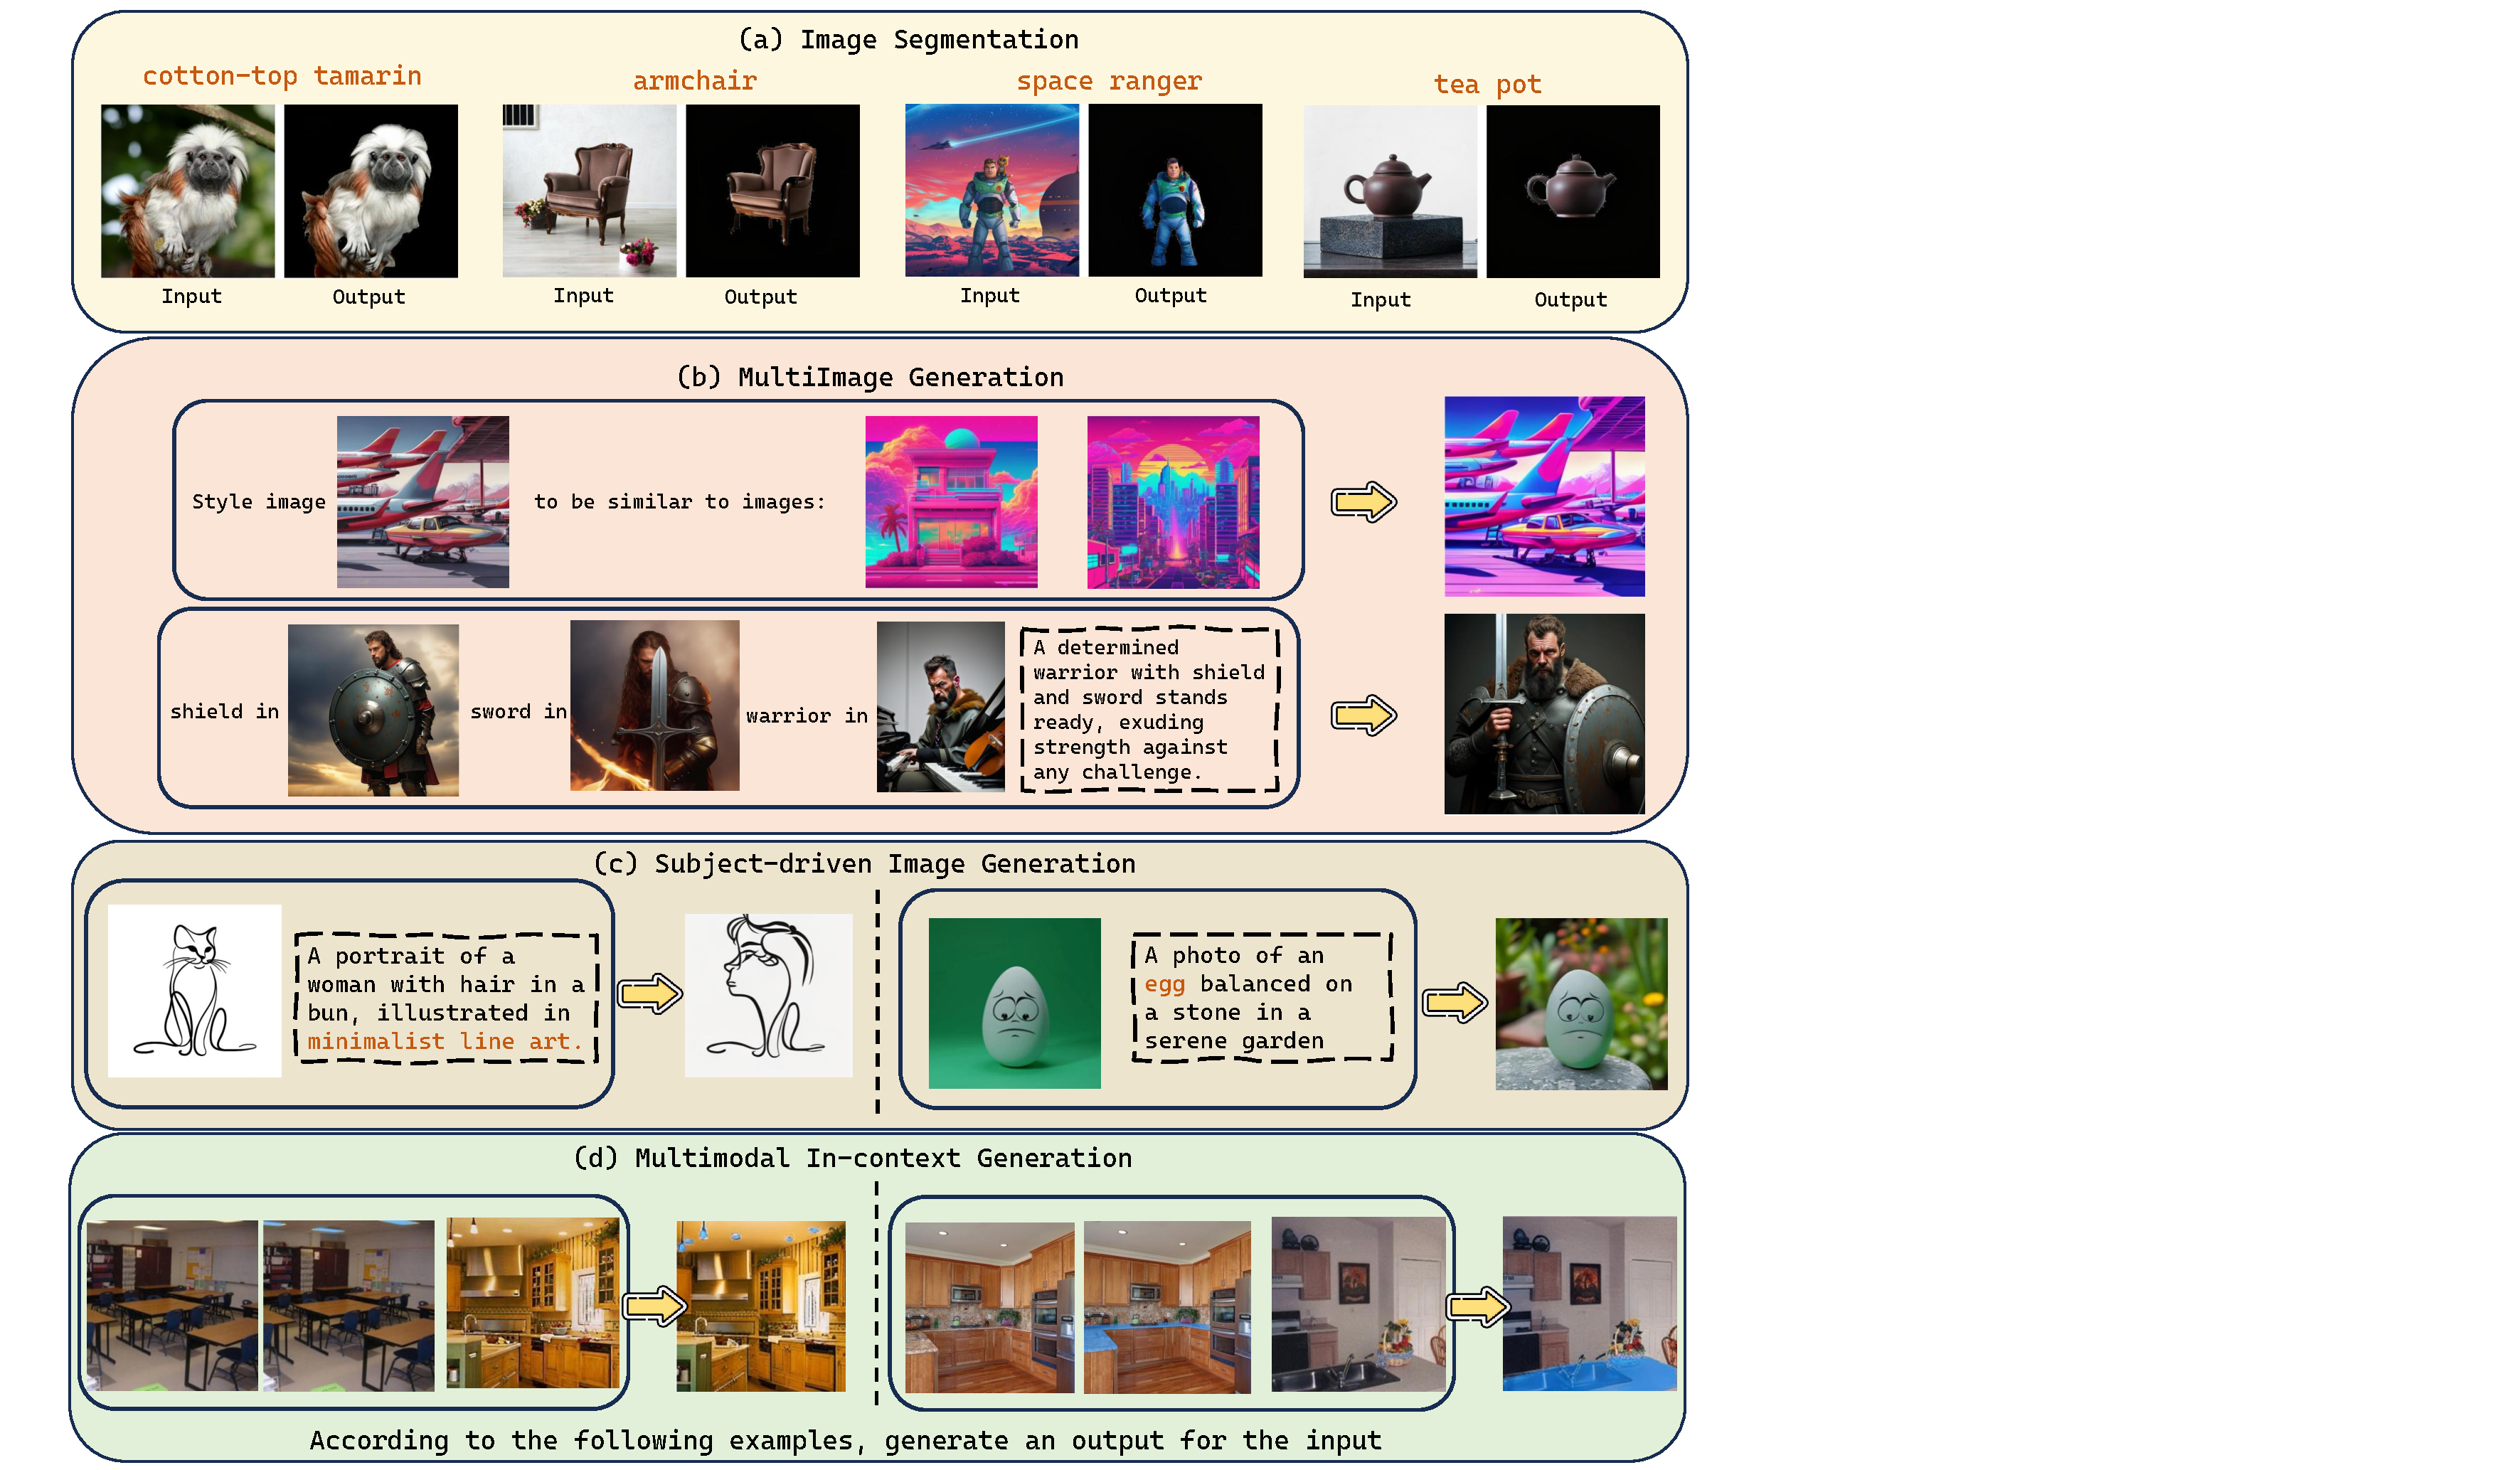
\includegraphics[width=1.0\textwidth]{figures/examples.pdf}
% 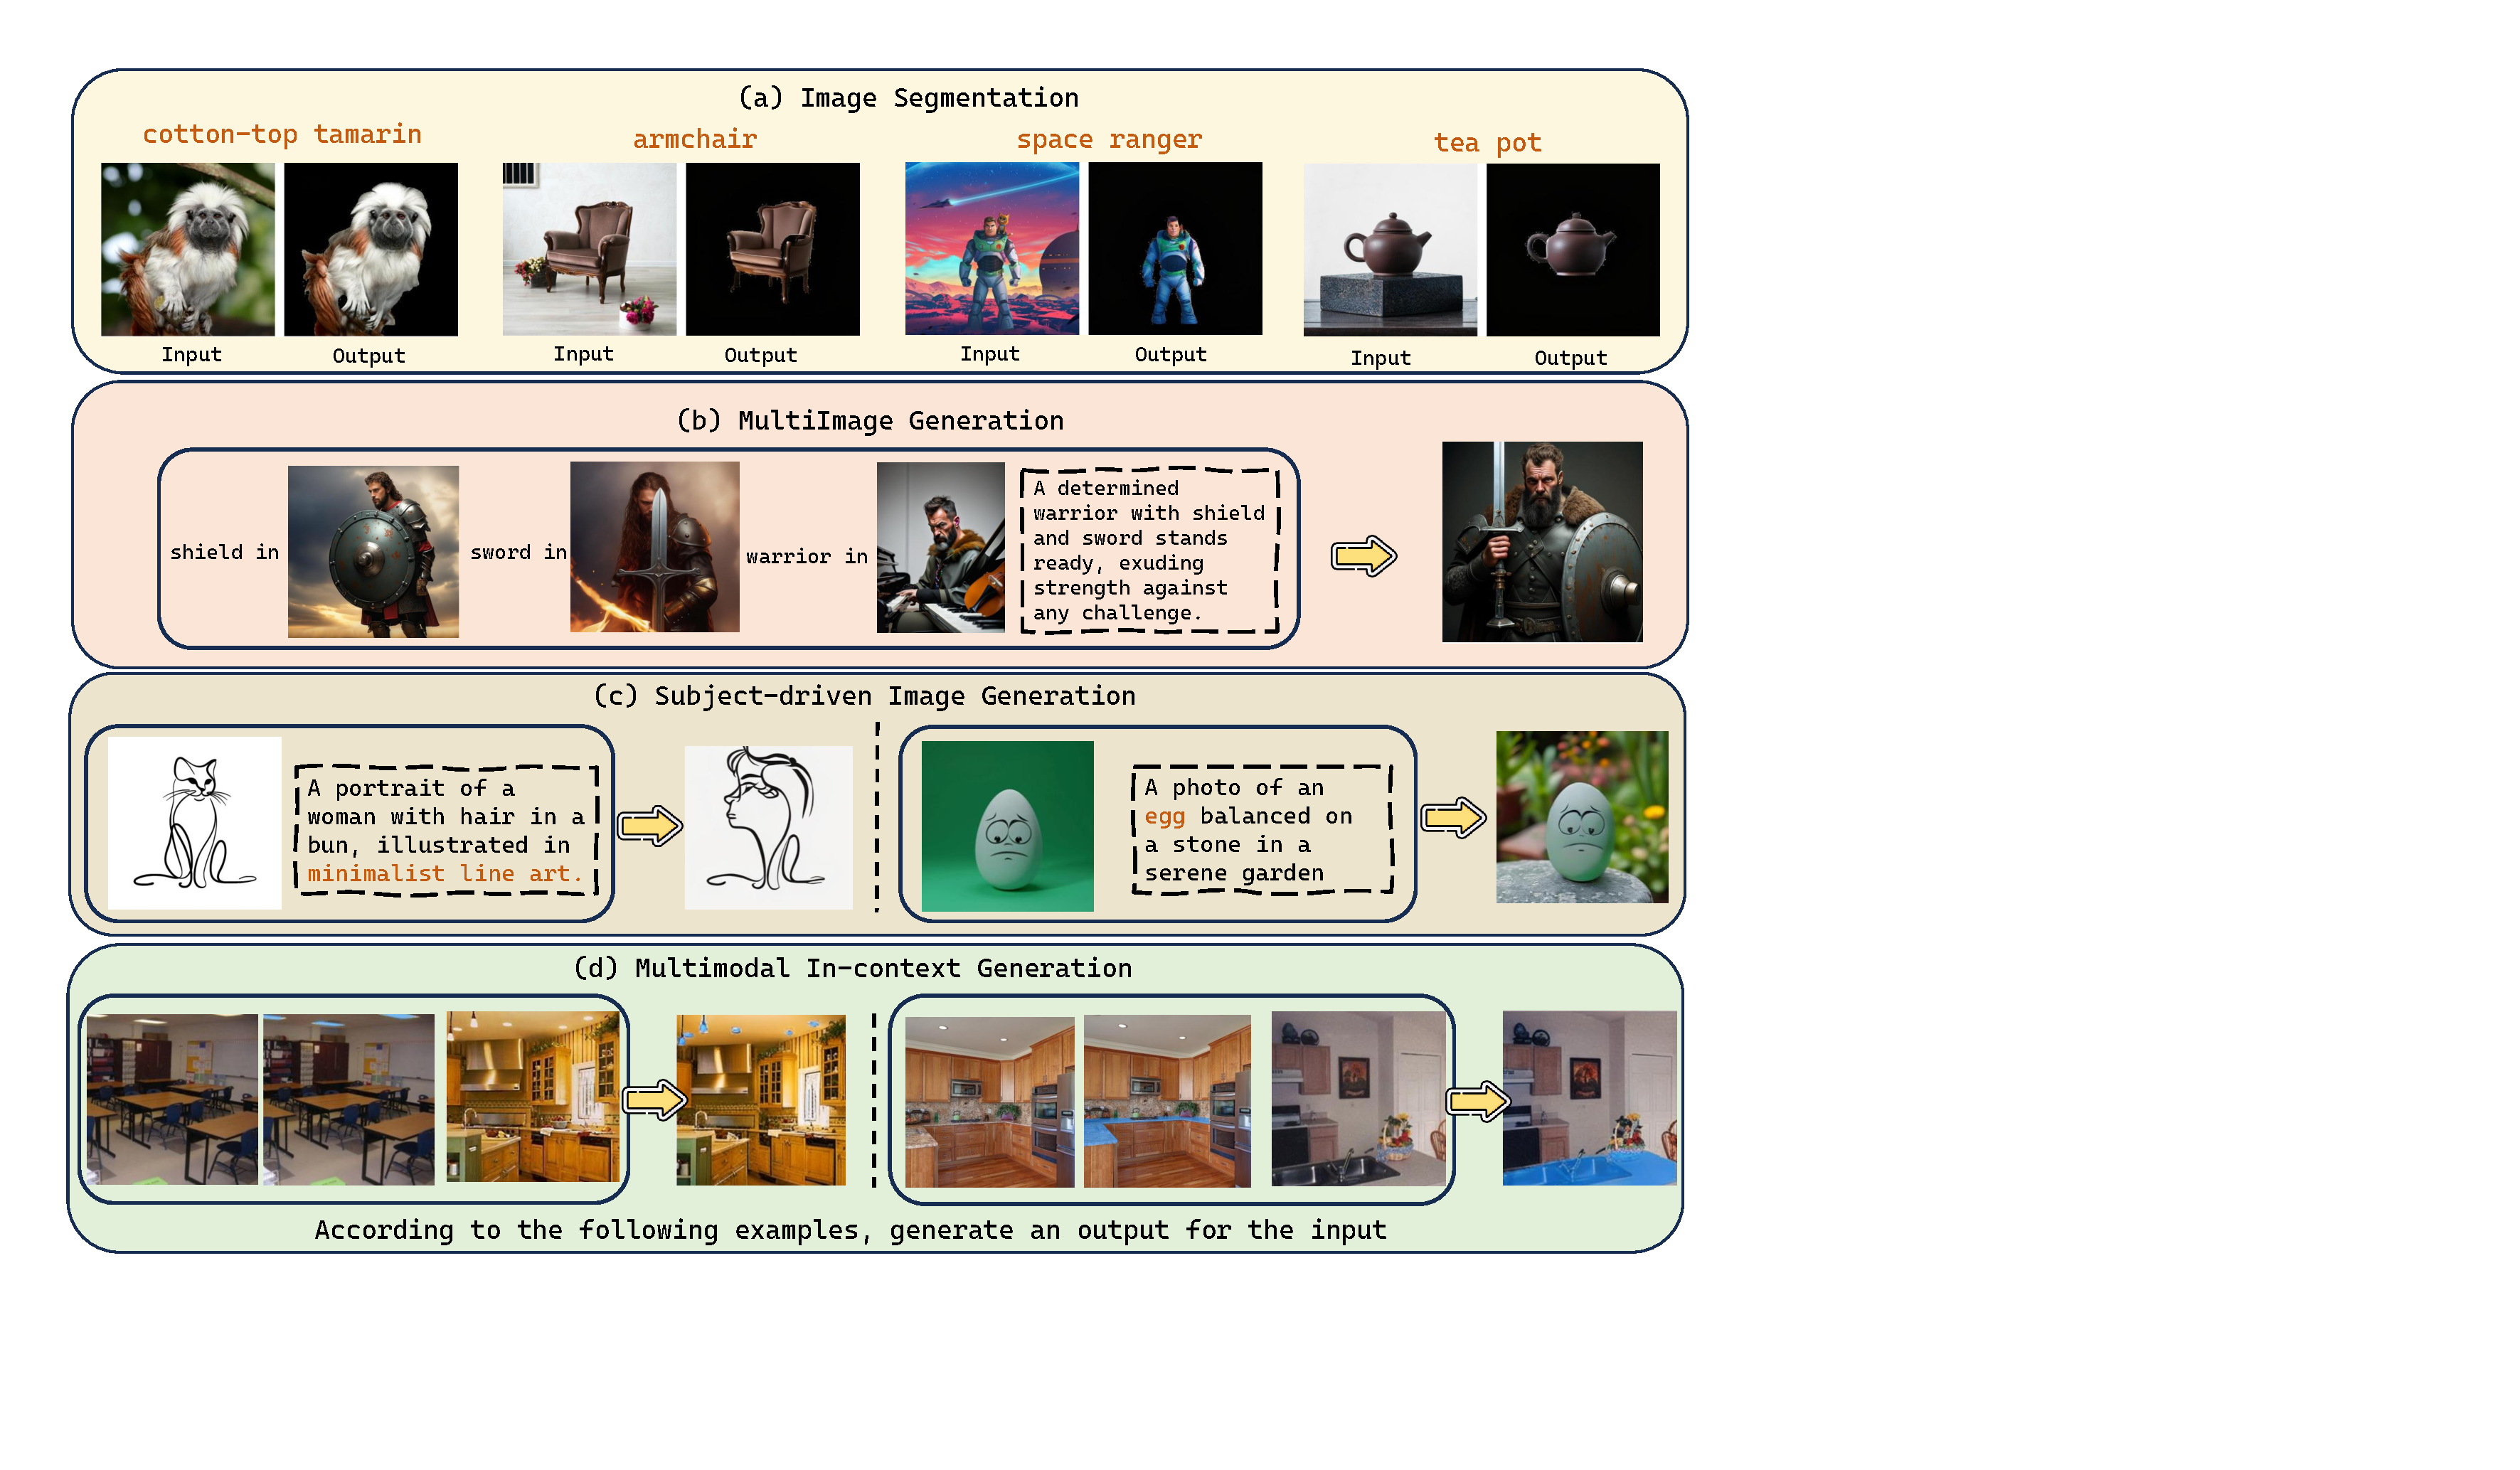
\includegraphics[width=0.7\textwidth]{figures/teasar.pdf}
% 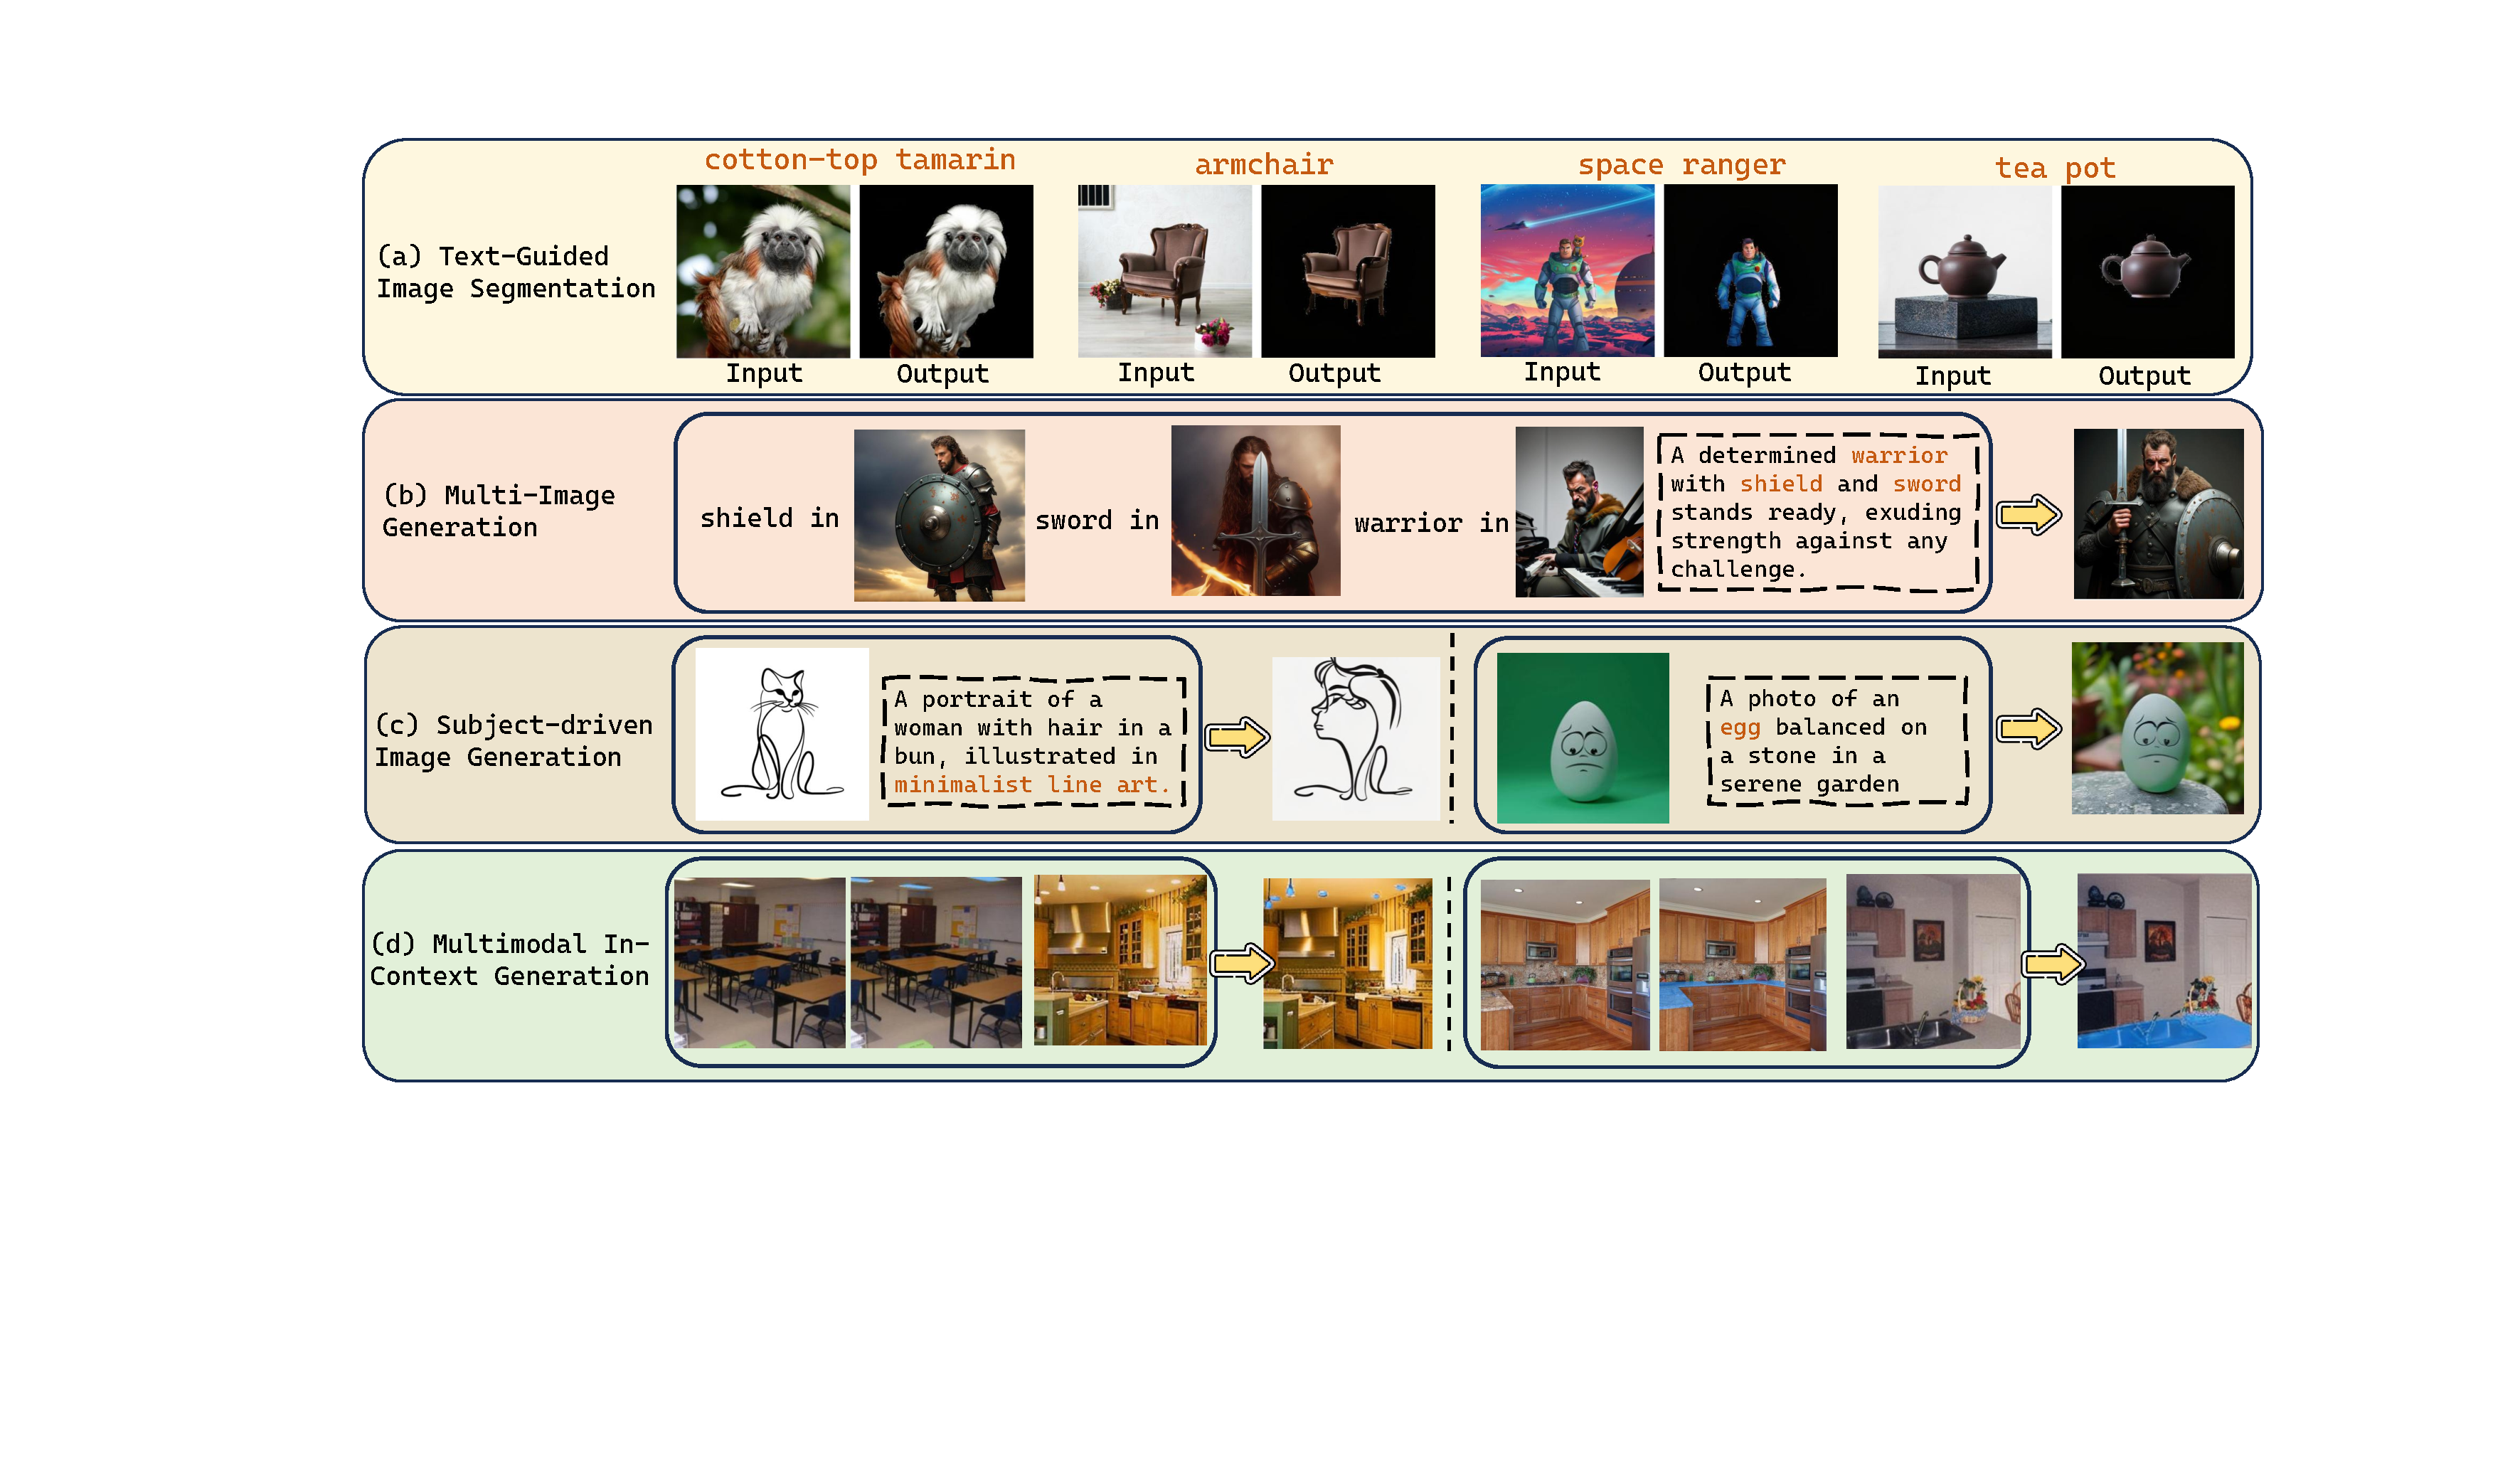
\includegraphics[width=0.9\textwidth]{figures/teasarv2.pdf}
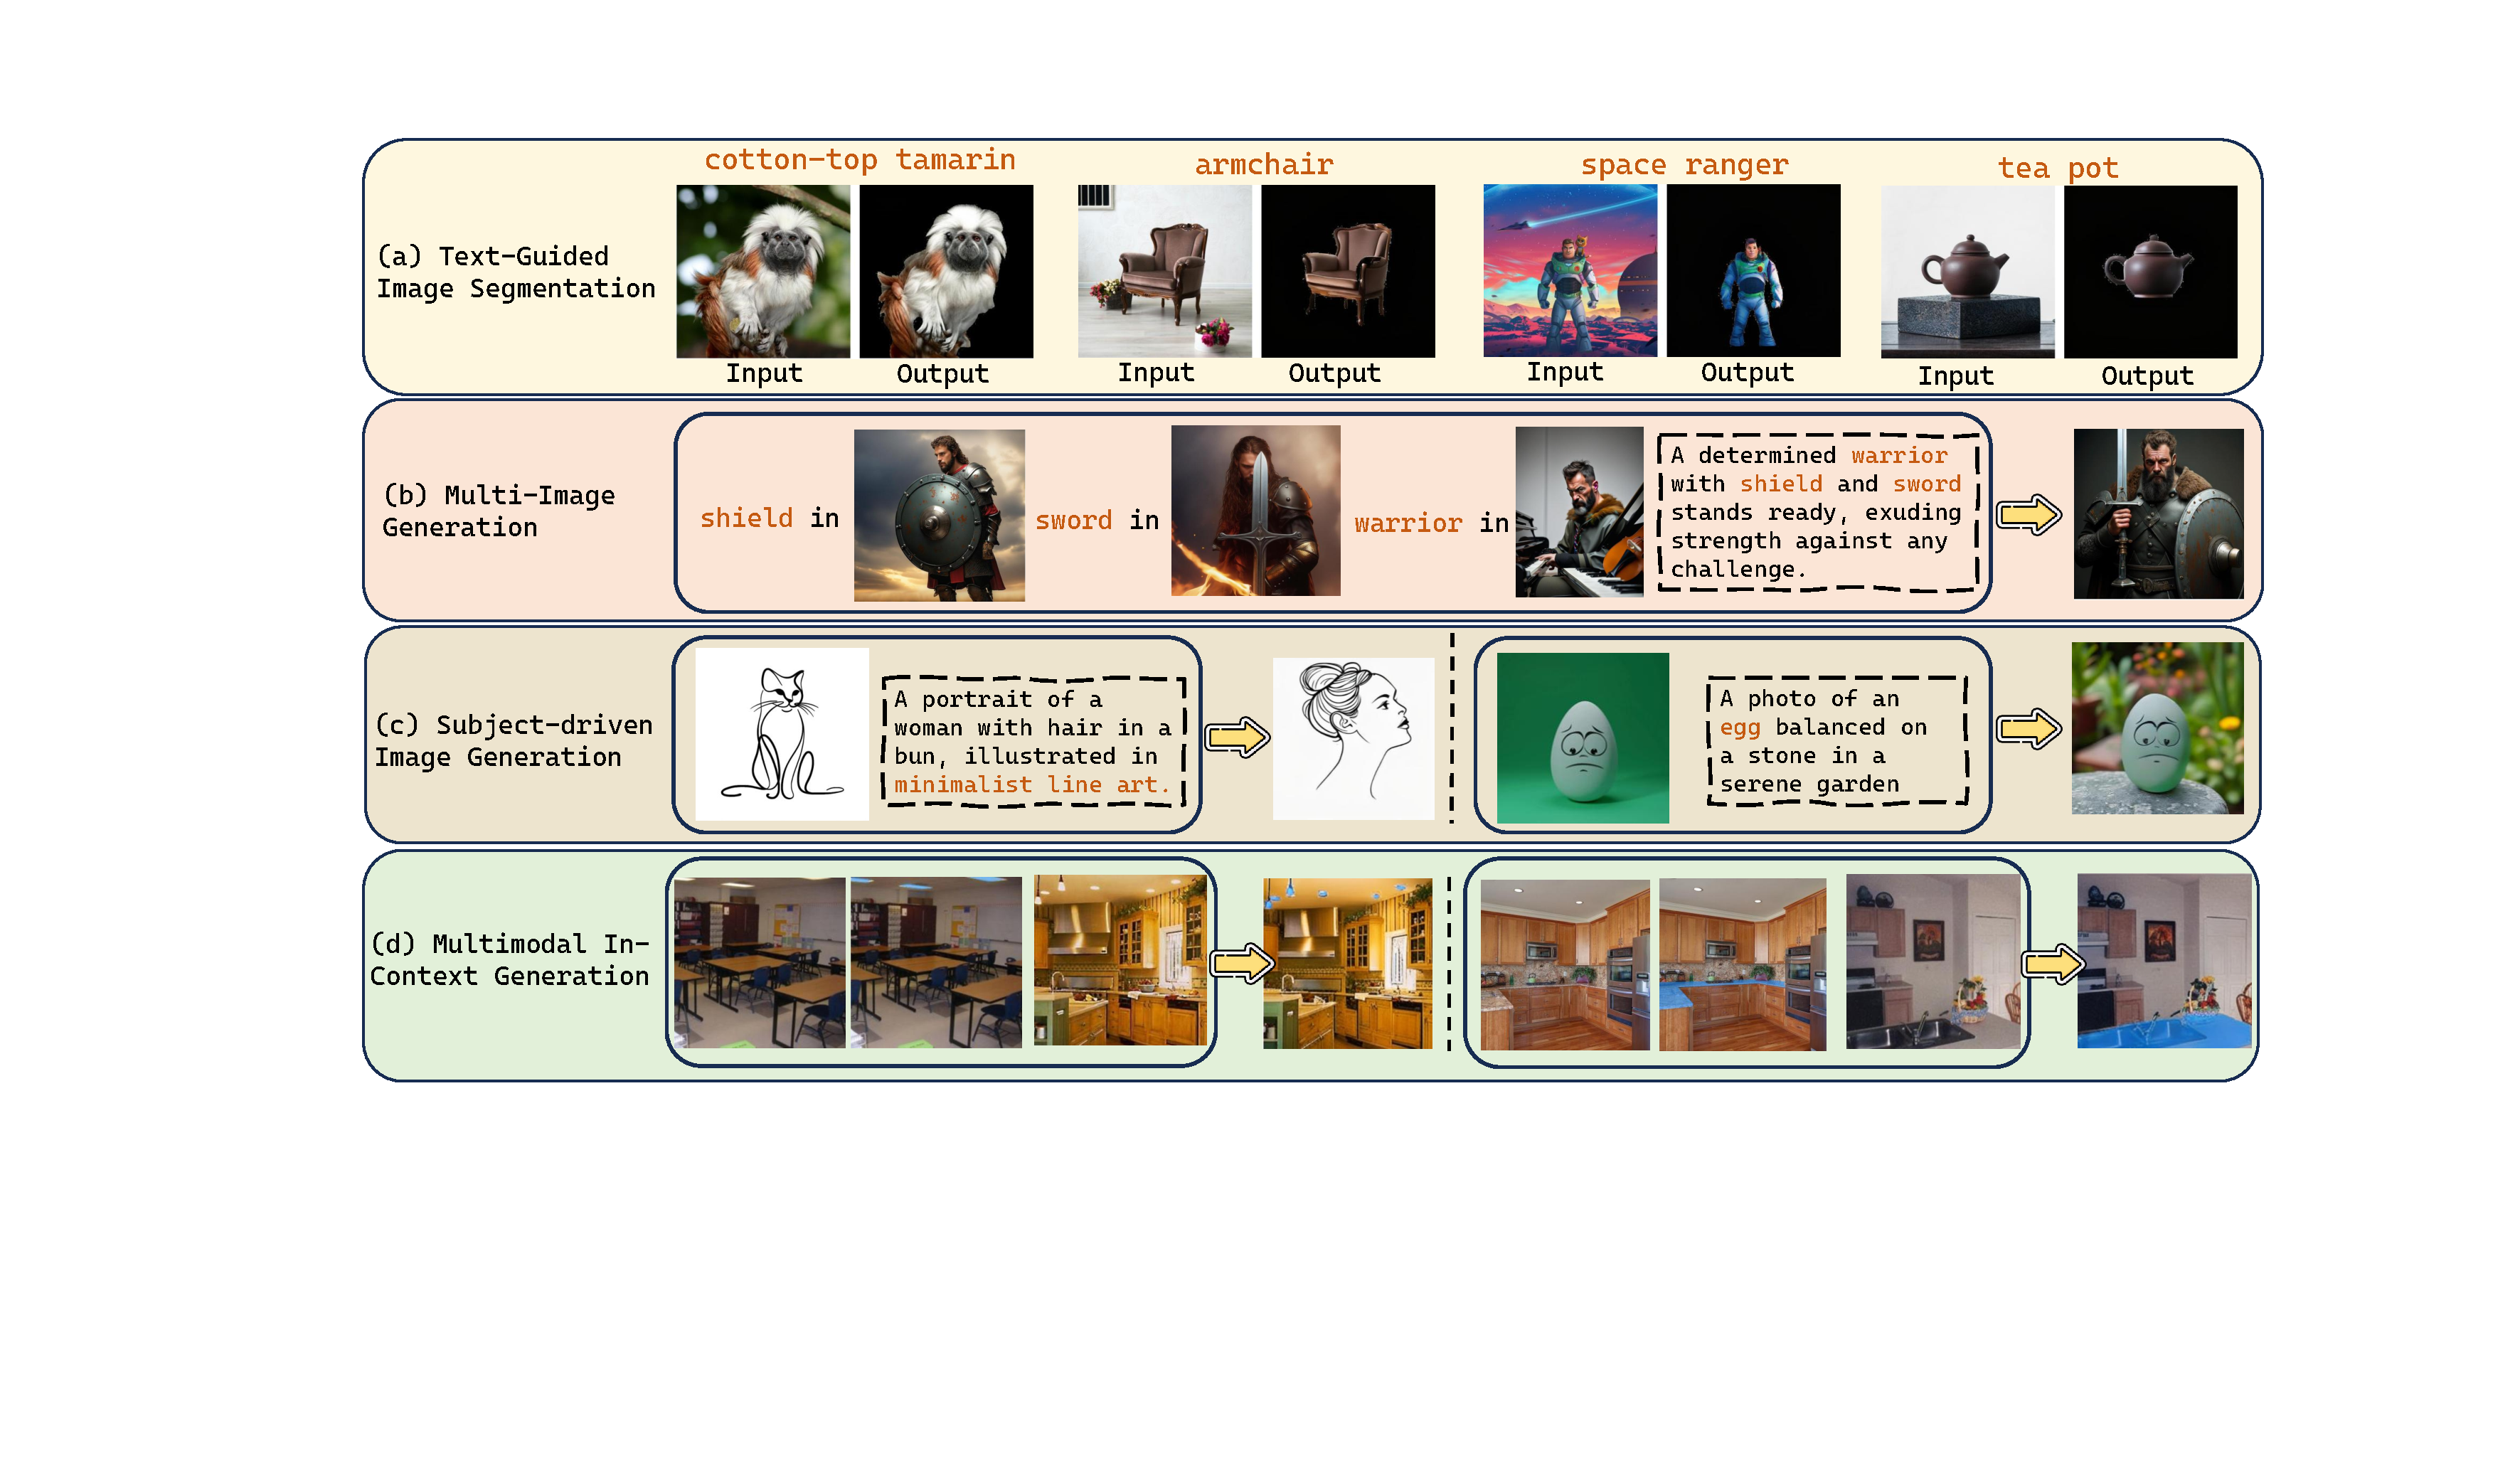
\includegraphics[width=0.9\textwidth]{figures/teasarv3.pdf}
\caption{Versatile applications built on \model after simply fine-tuning on corresponding datasets.
% , including (a) image segmentation, (b) multi-image generation, (c) subject-driven image generation, and (d) multimodal in-context learning image generation
}
\label{fig:examples}
\end{figure*}
\end{abstract}
% % 
\section{Introduction} 
\label{sec:introduction}
% \vspace{-1ex}
% \begin{figure}[t]
%     \centering
%     \begin{minipage}{0.45\textwidth}
%         \centering
%         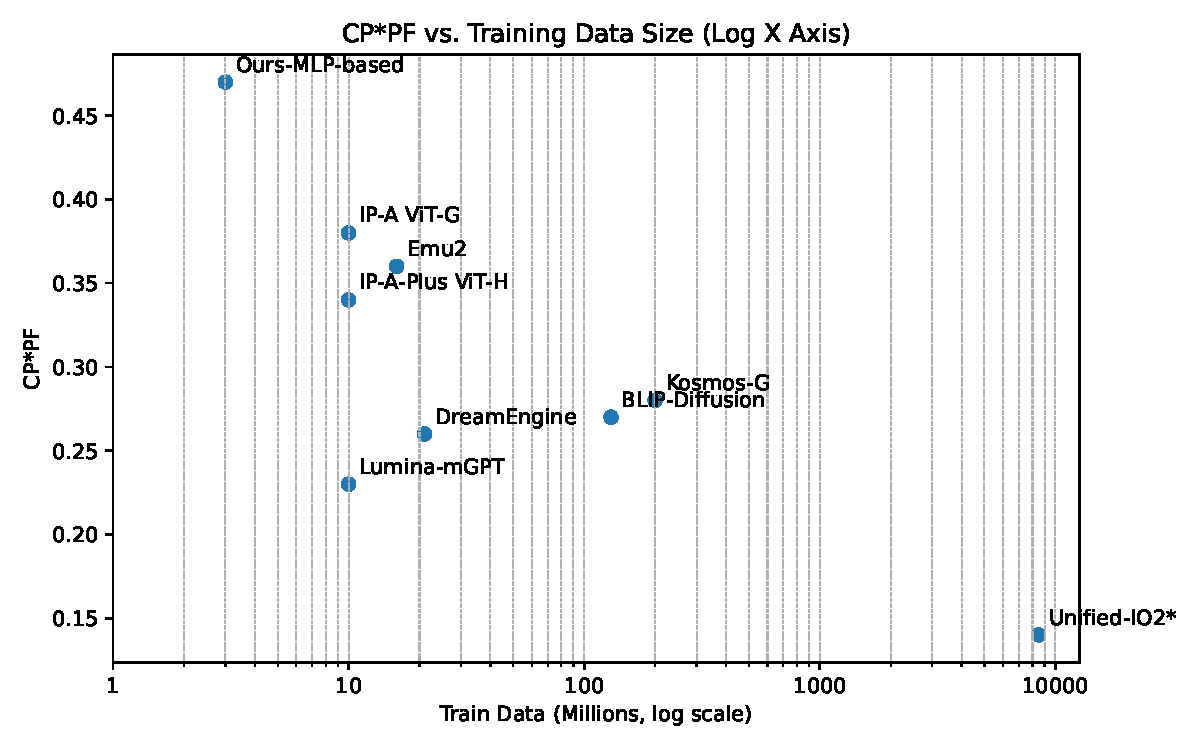
\includegraphics[width=\textwidth]{figures/data.pdf}
%         \caption{data}
%         \label{fig:data}
%     \end{minipage}
%     \hfill
%     \begin{minipage}{0.45\textwidth}
%         \centering
%         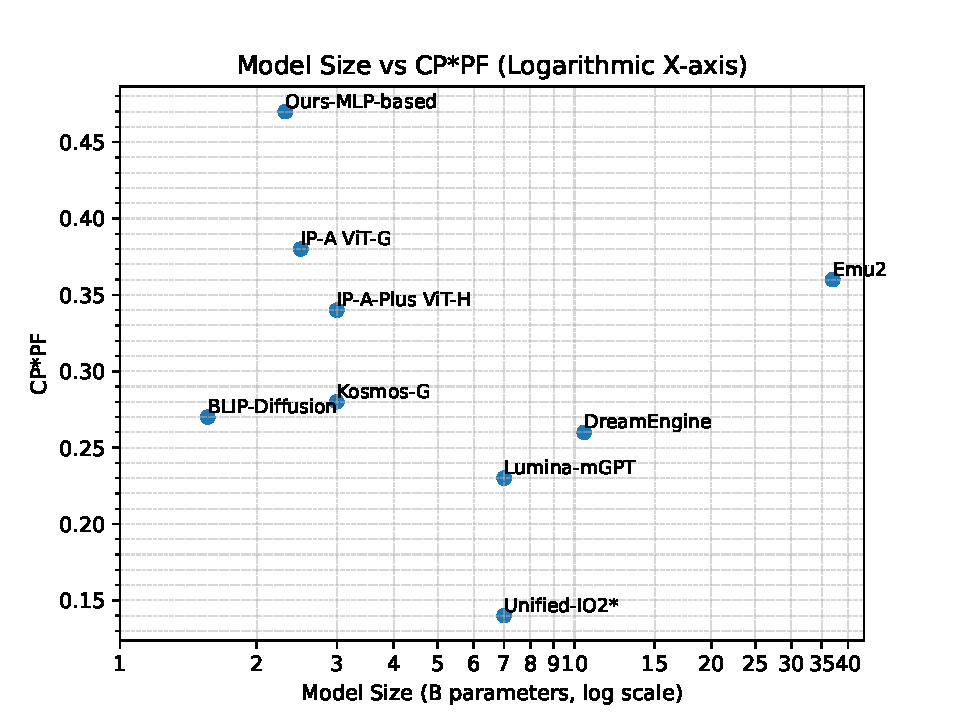
\includegraphics[width=\textwidth]{figures/size.pdf}
%         \caption{size}
%         \label{fig:size}
%     \end{minipage}
%     \caption{Caption text here}
%     \label{fig:comparison}
% \end{figure}

\begin{wrapfigure}{r}{0.50\textwidth} 
    \centering
    \vspace{-5mm}
    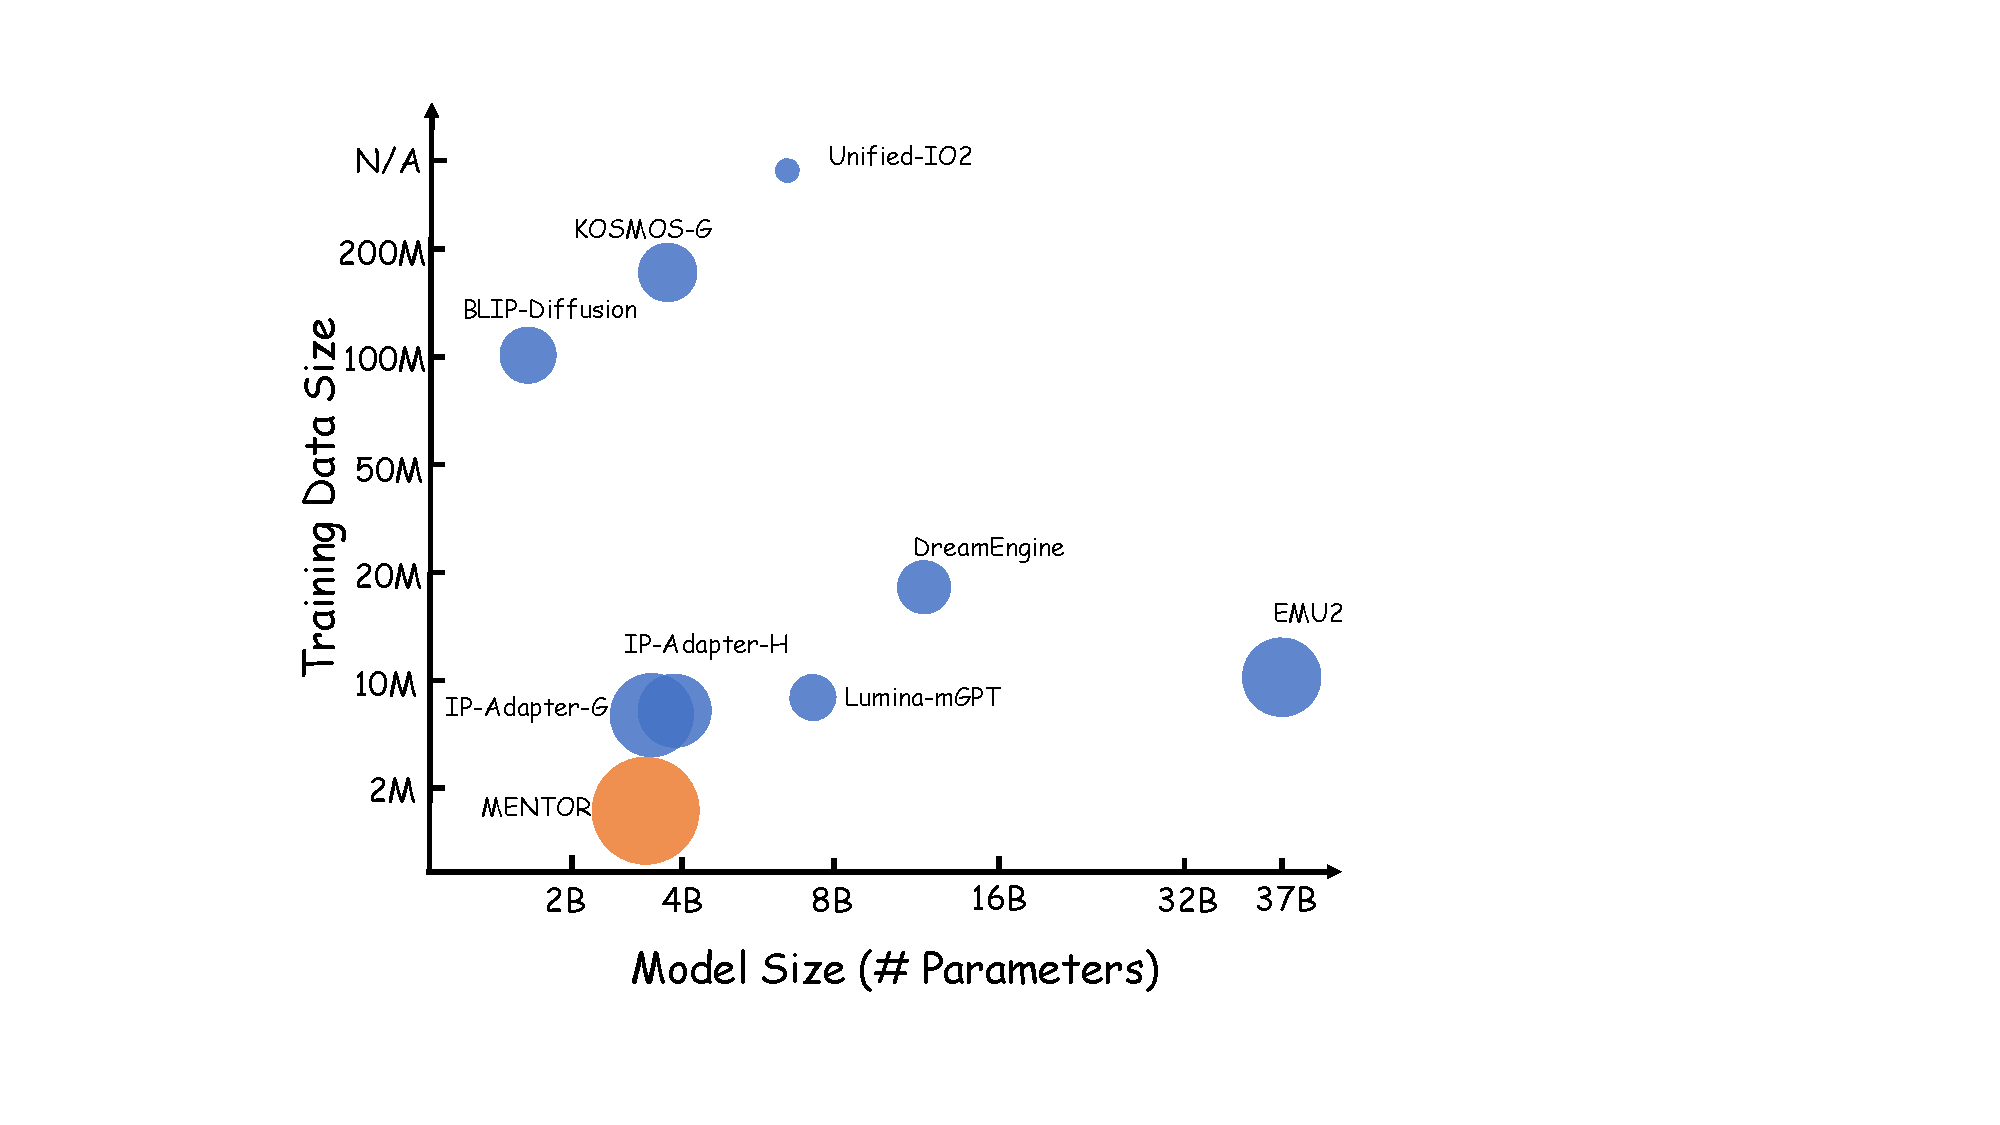
\includegraphics[width=\linewidth]{figures/Figure.pdf}
    % \caption{CP$\cdotp$PF score (circle size) of \model and other baselines on DreamBench++. Model in lower left achieves the best efficiency. }
    \caption{CP$\cdotp$PF score (circle size) of \textcolor[HTML]{ED8B50}{\textbf{\model}} and \textcolor[HTML]{5A76A9}{\textbf{other baselines}} on DreamBench++. Model in lower left achieves the best efficiency.}
    \label{fig:SnapKV}
    \vspace{-0.3cm}
\end{wrapfigure}



Recent progress in generative models has revolutionized text-to-image(T2I) generation~\citep{2020DDPM,ldm,SDXL}. However, real-world applications often require more than text-only prompts.
To achieve high-quality image generation, e.g., fine-grained control over generated images, the models need to seamlessly integrate multi-modal inputs, such as reference images with detailed instructions.
This poses significant challenges for existing diffusion models that are predominantly focused on T2I generation.
To address this, researchers have recently employed Large Multimodal Models (LMMs) to encode diverse inputs into unified embeddings compatible with diffusion models \citep{Kosmos-G, emu2}. While this approach aids in handling complex prompts for generation like interleaved image-text instructions \citep{emu2} or multimodal in-context learning \citep{Kosmos-G,2024SeedX}, several key limitations persist when scaling to complex multimodal control:

% Modern generative models have achieved remarkable success in image generation, with diffusion models leading the state-of-the-art performance in text-to-image generation~\citep{2020DDPM,ldm,SDXL}.
% Recent progress in generative models has revolutionized text-to-image generation with their remarkable capabilities\citep{2020DDPM,ldm,SDXL}.
% Along with their open-source communities, diffusion models dominate the field of visual generation up to today, particularly in text-to-image generation.
% However, real-world image generation applications often demand user interactions beyond simple text-only prompts. 
% To achieve high-quality image generation, e.g., fine-grained control over the generated images, the models need to seamlessly integrate multi-modal inputs, such as reference images, spatial layouts, stylistic exemplars, and detailed textual instructions.
% It poses significant challenges for existing diffusion models that are predominantly focused on text-to-image generation.

% Pervious methods have augmented diffusion models with auxiliary control mechanisms~\citep{controlnet, ye2023ip-adapter,ruiz2023dreamboothfinetuningtexttoimage}, enabling conditional generation guided by additional visual inputs. While effective in specific scenarios, these approaches often rely on task-specific adapters and specialized fine-tuning, which can limit their scalability and broader applicability. 
% Moreover, recent works integrate the large multimodal models (LMMs) with diffusion-based generators~\citep{Kosmos-G, emu2} to encode multimodal inputs into unified embeddings that are compatible with diffusion models, thereby supporting the multimodal conditional image generation.

% To address this challenge, early methods have augmented diffusion models with auxiliary control mechanisms.
% Approaches like ControlNet~\citep{controlnet} and DreamBooth~\citep{ye2023ip-adapter, ruiz2023dreamboothfinetuningtexttoimage} often rely on task-specific adapters and specialized fine-tuning, limiting their generalization ability.
% To address this challenge, more recently, researcher has leveraged Large Multimodal Models (LMMs) to encode diverse multimodal inputs into unified embeddings that are compatible with diffusion models~\citep{Kosmos-G, emu2}. This approach facilitates handling complex multimodal prompts, such as interleaved image-text instructions~\citep{emu2} or multimodal in-context learning~\citep{Kosmos-G,2024SeedX} for image generation.
% Nevertheless, despite their achievements, these methods still face several key limitations when scaled to complex multimodal control:





% To address this challenge, previous methods have augmented diffusion models with auxiliary control mechanisms, such as ControlNet~\citep{controlnet} and IP-Adapter~\citep{ye2023ip-adapter}~\citep{controlnet, ye2023ip-adapter,ruiz2023dreamboothfinetuningtexttoimage}, which often rely on task-specific adapters and specialized fine-tuning. 
% Moreover, others integrate Large Multimodal Models (LMMs) to encode diverse multimodal inputs into unified embeddings that are compatible with diffusion models~\citep{Kosmos-G, emu2}. These method aims to support more complex multimodal prompts, such as interleaved image-text instructions~\citep{emu2} or multimodal in-context learning~\citep{Kosmos-G,2024SeedX} for image generation.
% Despite promising in specific scenarios, these methods still face several key limitations when scaled to complex multimodal control:

% Despite these advances, existing methods still face significant challenges:
% \textbf{First}, the inherent randomness of diffusion processes complicates achieving precise and deterministic control, which is often necessary for tasks requiring high fidelity or accurate image reconstruction~\citep{wang2025imageeditingdiffusionmodels}. 
% \textbf{Second}, effectively balancing guidance of different modalities remains a persistent challenge. 
% Existing methods often struggle to integrate information harmoniously, sometimes over-emphasizing one modality while neglecting others~\citep{han2024emmatexttoimagediffusionmodel}. 
% For instance, methods like IP-Adapter~\citep{ye2023ip-adapter} and Lumina-mGPT~\citep{2024lumina}, which rely on text and image features as conditions, may predominantly be influenced by the image conditions.
% This imbalance can stem from the gap between modalities, which is further exacerbated by model architecture limitations~\citep{zhao2023mmicl,Dig2DIG,ye2023ip-adapter}, as well as suboptimal training paradigms~~\citep{Kosmos-G,han2024emmatexttoimagediffusionmodel}.
% \textbf{Third}, current diffusion-based methods~\citep{Kosmos-G,li2023blipdiffusionpretrainedsubjectrepresentation, emu2}, especially those incorporating auxiliary components for alignment(e.g., learned adapters~\citep{Kosmos-G}, regression heads~\citep{sun2023emu1,emu2}, specialized embeddings~\citep{seed-tokenizer}), typically necessitate extensive training on large-scale datasets~\citep{emu2,Kosmos-G,li2023blipdiffusionpretrainedsubjectrepresentation,2024SeedX}, incurring substantial computational costs.
% This is driven by the large parameter counts of individual components~\citep{emu2,Kosmos-G} (e.g., LLMs, diffusion backbones), auxiliary components, and the need for vast multimodal datasets.

\textbf{First,} the randomness of diffusion processes hinders precise, deterministic control, which is essential for high-fidelity tasks, like image reconstruction\citep{wang2025imageeditingdiffusionmodels}.
\textbf{Second,} balancing guidance from different modalities remains challenging. Existing methods frequently exhibit modality imbalance, often over-emphasizing one modality while neglecting others\citep{han2024emmatexttoimagediffusionmodel}. For instance, IP-Adapter \citep{ye2023ip-adapter} and Lumina-mGPT \citep{2024lumina}, conditioned on text and image features, may overly favor image inputs. This imbalance stems from modality gaps, architectural limitations \citep{zhao2023mmicl,Dig2DIG,ye2023ip-adapter}, or suboptimal training schemes \citep{Kosmos-G,han2024emmatexttoimagediffusionmodel}.
\textbf{Third,} many diffusion-based methods \citep{Kosmos-G, emu2}, particularly those with auxiliary alignment components (e.g., learned adapters \citep{Kosmos-G}, regression heads \citep{sun2023emu1,emu2}, specialized embeddings \citep{seed-tokenizer}), demand large-scale training \citep{emu2,Kosmos-G,li2023blipdiffusionpretrainedsubjectrepresentation,2024SeedX}, incurring substantial computational costs.
These challenges raise a critical question: \textit{Is there a more efficient and controllable paradigm for balancing complex multimodal conditions in image generation?}

% propose \textbf{\model}, a novel autoregressive (AR) framework for efficient \textbf{M}ultimodal g\textbf{E}neratio\textbf{N} \textbf{T}uning for aut\textbf{O}reg\textbf{R}essive multimodal image generation.
To address aforementioned limitations, we propose \textbf{\model}, a straightforward and efficient autoregressive (AR) framework for controllable multimodal image generation. Unlike diffusion models that rely on complex cross-attention layers for multimodal conditioning and demand extensive training resources \citep{2024SeedX,emu2,Kosmos-G,li2023blipdiffusionpretrainedsubjectrepresentation},  \model leverages a unified transformer architecture that directly aligns multimodal inputs with output image tokens. This design inherently simplifies architecture and training, reduces the need for auxiliary components for alignment, and significantly lowers training requirements.
Our framework employs a multimodal encoder to project multimodal inputs into a unified representation. An AR transformer decoder then generates image tokens deterministically, conditioned on this representation. To ensure effective and balanced modality integration, which is curial for multimodal image generation\citep{han2024emmatexttoimagediffusionmodel}, we adopt a two-stage training paradigm: (1) pretraining on image reconstruction and object segmentation to enable robust pixel-level and semantic alignment, followed by (2) multimodal instruction tuning with diverse tasks, such as image recovery and subject-driven generation, explicitly training the model to effectively leverage and balance varied multimodal inputs for coherent generation.

Notably, despite its simplicity and the use of suboptimal checkpoints, \model achieves state-of-the-art(SOTA) performance on the challenging DreamBench++ benchmark—using 10× less training data than leading baselines.
It outperforms resource-intensive baselines with powerful generators like SDXL \citep{SDXL} and SD3 \citep{2024SD3} by 30\% while dramatically reducing computational and data demands. 
Controlled experiments demonstrate the advantages of \model over diffusion-based methods in multimodal fidelity, training efficiency, and generation controllability.


 
% even with readily available multimodal encoders and modestly-sized autoregressive decoders, our method achieves state-of-the-art performance on the challenging DreamBench++ benchmark. It significantly surpasses resource-intensive baselines utilizing powerful generators like SDXL \citep{SDXL} and SD3 \citep{2024SD3} by 30\% while dramatically reducing computational and data demands. Extensive controlled experiments validate our AR approach's compelling advantages in multimodal fidelity, training efficiency, and generation controllability.

% In this paper, we propose a straightforward and efficient autoregressive (AR) framework explicitly designed for controllable multimodal image generation, directly addressing key limitations of prevalent diffusion-based approaches.
% including an AR generation model that suports multimodal conditions and a meticulously designed two-stage training paradigm.
% In contrast to diffusion-based methods that use cross-attention layers for multimodal conditioning and require extensive GPU resources for training, our approach directly aligns multimodal inputs with generated output tokens through unified autoregressive modeling in a simple transformer framework. It facilitates direct, token-level alignment between multimodal conditions and the generated image, providing a direct pathway for integrating diverse inputs.
% This inherent simplicity significantly reduces the reliance on task-specific adapters or extensive auxiliary components, leading to substantially lower training requirements.
% In contrast to diffusion-based methods that employ cross-attention layers for multimodal conditioning and typically necessitate extensive GPU resources for their training phases\citep{2024SeedX,emu2,Kosmos-G,li2023blipdiffusionpretrainedsubjectrepresentation}, our proposed method utilizes unified autoregressive modeling within a transformer architecture. This allows for the direct alignment of multimodal inputs with generated output tokens. 
% Such a direct pathway inherently simplifies the model architecture. 
% Consequently, it reduces the reliance on task-specific adapters or extensive auxiliary components for alignment and has significantly reduced training requirements.


% over diffusion-based counterparts.


% While pervious works like llamaGen~\citep{llamagen}, VILA-U~\citep{VILA-U}, EMU3~\citep{Emu3}, and the Janus-Series~\citep{Janus} have delved into autoregressive text-to-image generation, their capabilities for handling intricate multimodal conditions remain largely unexplored. 
% In contrast, our approach distinctively addresses multimodal conditional generation through the proposed AR framework and a carefully designed two-stage multimodal instruction tuning process. 
% By uniformly handling visual and textual inputs within a sequence-to-sequence modeling framework, our method paves the way towards more efficient, controllable, and robust multimodal generative systems.

% Through this implicit cross-modal alignment, achieved via token-level interactions, our approach substantially reduces the reliance on specialized modality adapters or extensive auxiliary components.
% This inherent simplicity translates directly into significantly reduced training requirements.
% Furthermore, to prevent the model from defaulting to a simple copy-paste function~\citep{han2024emmatexttoimagediffusionmodel} and overlooking textual conditions, our two-stage training process and diverse tasks ensure a nuanced understanding of visual input and a balanced integration of all modalities.


% Our framework utilizes a multimodal encoder to project heterogeneous inputs (visual and textual) into a unified latent space. An autoregressive transformer decoder then deterministically generates image tokens based on this unified representation. 
% To ensure robust understanding and balanced integration of diverse modalities—specifically preventing the model from defaulting to simple copy-paste function~\citep{han2024emmatexttoimagediffusionmodel} while ignoring textual instructions—we introduce a carefully designed two-stage training paradigm. In the first stage, the model is pretrained on image reconstruction and object segmentation tasks, fostering robust pixel-level and semantic-level alignment between the multimodal input and generated tokens. Subsequently, the second stage involves multimodal instruction tuning with diverse tasks, such as image recovery and subject-driven generation. This stage explicitly trains the model to leverage varied multimodal inputs effectively while balancing its focus across different modalities for coherent image generation.



% Specifically, our method employs a multimodal encoder to project heterogeneous inputs—visual and textual data—into a unified latent embedding space, creating a comprehensive multimodal representation. An autoregressive transformer-based decoder subsequently generates images based on this representation, producing deterministic outputs that accurately reflect the provided conditions.
% Building upon this architecture, we introduce a meticulously designed two-stage training paradigm. In the first stage, the model is pretrained on image reconstruction and object segmentation tasks, fostering robust pixel-level and semantic-level alignment and encouraging effective exploitation of visual information for image synthesis. 
% Subsequently, we perform the multimodal instruction tuning that incorporates additional training tasks, such as image recovery and subject-driven image generation. The second stage empowers the model to leverage varied multimodal inputs for image generation while explicitly balancing its focus across different modalities, enabling an efficient and robust fusion of multimodal information into coherent image outputs.

% Remarkably, even when employing readily available multimodal encoders and modestly-sized autoregressive decoders, our method achieves state-of-the-art performance on the challenging DreamBench++ benchmark. It surpasses the resource-intensive baselines, which utilize much more power generators like SDXL~\citep{SDXL} and SD3~\citep{2024SD3}, by xx\% while dramatically reducing computational and data resource demands. Through extensive controlled experiments, we directly compare our AR approach with diffusion-based counterparts and demonstrate compelling advantages in multimodal fidelity, training efficiency, and generation controllability.

% our method surpasses other baselines and achieves state-of-the-art performance on the challenging DreamBench++ benchmark by xx\%, while dramatically reducing computational and data resource demands. We also conduct extensive controlled experiments comparing our autoregressive approach directly with diffusion-based paradigms. 
% Our findings demonstrate that autoregressive models offer significant advantages in multimodal fidelity, generation controllability, and consistency.


% Our contributions are summarized as follows:
% \begin{itemize}[left=2pt]
% \item We propose a novel autoregressive framework for efficient multimodal image generation tuning, demonstrating state-of-the-art performance with substantially reduced training resources.
% \item We introduce a two-stage training strategy to align multimodal embeddings effectively, enabling balanced multimodal attention and precise conditional adherence.
% \item Extensive experiments validate the superior efficiency and multimodal capabilities of our AR framework, highlighting its potential as a scalable alternative to existing diffusion-based methods.
% \end{itemize}
Overall, our contributions are as follows: (1) A novel autoregressive framework for efficient multimodal generation, achieving, achieving SOTA performance; (2) A two-stage training strategy for multimodal-conditioned tuning, enabling robust alignment and balanced modality integration with significantly reduced training cost; (3) Extensive experiments demonstrating the superior efficiency, controllability, and fidelity of \model as a compelling alternative to diffusion-based methods.



% Our contributions are:
% \begin{itemize}[left=2pt]
%     % \setlength\itemsep{0.1em}
%     \item A novel autoregressive framework for efficient and controllable multimodal  generation, achieving state-of-the-art performance with substantially reduced training resources.
%     \item A two-stage training strategy to ensure robust multimodal alignment and balanced integration of diverse modalities for controllable multimodal image generation.
%     \item Extensive experiments validating the superior efficiency, controllability and multimodal fidelity of \model, highlighting its potential as a scalable alternative to the diffusion-based methods.
% \end{itemize}



% The proposed model integrates a multimodal encoder with a unified transformer decoder. The multimodal encoder is responsible for processing and fusing multimodal inputs into a coherent conditioning representation. It converts each input into combined latent token sequence for generation. This encoded sequence of tokens serves as deterministic context for the decoder. The unified transformer decoder then autoregressively generates the output image token-by-token. 

% Thanks to this design, our model can seamlessly integrate information from multimodal conditions and synthesize a new image that precisely reflects all these inputs, leading to three key advantages:

% \begin{itemize} 
% \item \textbf{Deterministic Control.} The absence of stochastic sampling enables consistent and interpretable outputs, supporting precise image reconstruction and fine-grained editing.
% \item \textbf{Multimodal Instruction Following.} Both language and vision are treated uniformly as token sequences, enabling seamless cross-modal attention and better instruction following for image generation. 
% \item \textbf{Training Efficiency.} Unified autoregressive modeling facilitates the direct alignment of multimodal inputs with output sequences. This implicit shortcut reduces reliance on modality-specific alignment modules, and also significantly lowers training costs.
% \end{itemize}



% Our AR model achieves state-of-the-art performance on the DreamBench++ benchmark, outperforming prior diffusion-based methods. Notably, our approach attains this strong performance with far fewer resources. In fact, even with sub-optimal large multimodal modules as the encoder and a relatively low-capacity image decoder, our AR framework matches surpasses other baselines. This highlights the training efficiency and effectiveness of our proposed paradigm – by treating generation as a discrete sequence prediction, we sidestep the need for large training data and lengthy training schedules, yet still capture the complex relationships between multimodal inputs and outputs.

% Furthermore, we conduct extensive controlled experiments to directly compare the AR and diffusion paradigms in multimodal conditional generation scenarios
% Our findings reveal that autoregressive models offer a promising and underexplored alternative for conditional image generation, particularly in multimodal settings requiring fine-grained control and interpretability. By unifying visual and text inputs in a sequence-to-sequence formulation, our approach paves the way toward more controllable and efficient generative systems.



% efficiency : model size training data

% % % \section{Preliminary}
\label{sec:preliminary}

\subsection{Model Design}


% % \section{Method}
\label{sec:method}


% This section details our proposed autoregressive framework for multimodal conditional image generation, its core components, two-stage training paradigm, and the data construction pipeline. 
This section details an efficient autoregressive framework for controllable multimodal image generation, achieving precise image control and balancing guidance across multiple modalities with minimal cost.
\Cref{sec:Preliminary} describes the autoregressive training objective for our framework. Next, \Cref{sec:model} presents a straightforward yet efficient model architecture, detailing how the framework accommodates multimodal inputs and supports autoregressive generation.
Crucially, \Cref{sec:traing_stages} introduces a two-stage training paradigm aimed at balancing the influences of different modalities during image generation.
Finally, \Cref{sec:data_construct} describes our automated pipeline for scalable multimodal data curation.

\subsection{Preliminary}
\label{sec:Preliminary}
\textbf{Training Objective}
Our model employs \emph{teacher forcing} to predict image tokens, conditioned on (i) previously generated tokens and (ii) multimodal context $\mathbf{h}$. 
Given the multimodal condition: $\mathbf{c}^{(0)} = \{\mathcal{I}, \mathcal{T}\}$ (visual and textual inputs),
a multimodal encoder~\(\phi\) first encodes $\mathbf{c}^{(0)}$ and subsequently uses an MLP layer to project them into space of the image decoder to form a unified representation $\mathbf{h}$:
\begin{equation}
    \mathbf{H} = \text{MLP}(\phi\bigl(\mathbf{c}^{(0)}\bigr))
    = (\mathbf{h}_1, \dots, \mathbf{h}_{M}) \in \mathbb{R}^{M\times d}, \qquad \mathbf{h}_j \in \mathbb{R}^{d}.
    \label{eq:enc}
\end{equation}
where $M$ is the number of conditioning tokens, and $d$ is the dimension of the latent embeddings.
% The autoregressive decoder $\theta$, conditioned on $\mathbf{h}$, generates an image token sequence $\mathbf{y} = (y_1, \dots, y_{L})$ of length $L$. Its conditional distribution factorizes as:
Then, the AR decoder $\theta$, conditioned on $\mathbf{h}$, generates image sequence $\mathbf{y} = (y_1, \dots, y_L)$ as follows:
\begin{equation}
    \small
    \theta(\mathbf{y} \mid \mathbf{H}) = \prod_{i=1}^{L} \theta\bigl(y_i \mid y_{<i}, \mathbf{H}\bigr).
    \label{eq:factor}
\end{equation}
% where $y_{<i} = (y_1, \dots, y_{i-1})$ are the preceding tokens.
The training objective is to minimize the token-level cross-entropy loss by \emph{teacher forcing} on data $\mathcal{D}$:
\begin{equation}
\small
    \mathcal{L}_{\text{CE}}(\theta, \phi)
    = -\mathbb{E}_{(\mathbf{y}, \mathbf{c}^{(0)}) \sim \mathcal{D}}
    \left[
        \sum_{i=1}^{L}
        \log \theta\bigl(y_i \mid y_{<i}, \mathbf{H} \bigr)
    \right].
    \label{eq:ce}
\end{equation}
% Our model is trained using \emph{teacher forcing} to predict image tokens, conditioned on (i) previously generated tokens and (ii) multimodal context provided by multimodal encoder.

% Formally, given the initial multimodal condition: $\mathbf{c}^{(0)} = \{\mathcal{I}, \mathcal{T}\}$, where $\mathcal{I}$ and $\mathcal{T}$ represent visual and textual inputs, respectively. To transform the multimodal inputs $\mathbf{c}^{(0)}$ into a unified representation $\mathbf{h}$, the multimodal encoder~\(\phi\) first encodes the input into conditioning hidden states and subsequently projects them into the latent embedding space of the decoder via a MLP projection layer:

% \begin{equation}
%    \mathbf{h} = \text{MLP}(\phi\bigl(\mathbf{c}^{(0)}\bigr))
%    = (h_1, \dots, h_{M}), \qquad h_j \in \mathbb{R}^{d},
%    \label{eq:enc}
% \end{equation}
% where $M$ is the number of conditioning tokens, and $d$ is the dimensionality of the latent embeddings. 

% The autoregressive decoder $\theta$ receives the sequence $\mathbf{h}$ as a prefix and generates an output sequence of image tokens $\mathbf{y} = (y_1, \dots, y_{L})$, where $L$ is the length of the target image-token sequence. The conditional distribution modeled by the decoder factorizes autoregressively as:
% \begin{equation}
%    \theta(\mathbf{y} \mid \mathbf{h})
%    = \prod_{i=1}^{L}
%    \theta\bigl(y_i \mid y_{<i}, \mathbf{h}\bigr),
%    \label{eq:factor}
% \end{equation}
% where $y_{<i} = (y_1, \dots, y_{i-1})$ denotes the previously generated tokens.

% Training is performed using \emph{teacher forcing}, where ground-truth prefix tokens are provided at each step. The objective is to minimize the token-level cross-entropy loss over the data distribution $\mathcal{D}$:
% \begin{equation}
%    \mathcal{L}_{\text{CE}}(\theta, \phi)
%    = -\mathbb{E}_{(\mathbf{y}, \mathbf{c}^{(0)}) \sim \mathcal{D}}
%    \left[
%       \sum_{i=1}^{L}
%       \log \theta\bigl(y_i \mid y_{<i}, \phi(\mathbf{c}^{(0)})\bigr)
%    \right].
%    \label{eq:ce}
% \end{equation}
\textbf{Classifier-free Guidance} 
To enhance multimodal generation controllability, we apply Classifier-Free Guidance (CFG)~\citep{llamagen}. During training, multimodal conditioning \(\mathbf{H}\) is replaced by a learned unconditional embedding \(\mathbf{H}_u\) with probability \(p\). At inference time, token logits \(\ell_g\) are recalculated by interpolating between the conditional logits \(\ell_c\) (from \(\mathbf{H}\)) and unconditional logits \(\ell_u\) (from \(\mathbf{H}_u\)), controlled by a scaling parameter \(\lambda\):
\(\ell_g = \ell_u + (\ell_c - \ell_u) \times \lambda\).





% To enhance the multimodal conditional generation capabilities of the model, following pervious methods~\citep{llamagen}, we integrate \emph{classifier-free guidance} (CFG) during both training and inference phases. 
% Specifically, during training, we randomly replace the original multimodal inputs $c$ with learnable conditional embeddings $u$ with the possibility $p$. 
% % to encourage the model to generalize beyond strict reliance on provided conditions. 
% At inference time, the logits for each predicted token are recalculated by interpolating between the conditional logits $\ell_{c}$ obtained from original multimodal conditions $c$ and unconditional logits $\ell_{u}$ derived from the learned conditional embeddings $u$, controlled by a scaling parameter $\lambda$:
% \begin{equation}  
% \ell_{g} = \ell_{u} + (\ell_{c} - \ell_{u}) \times \lambda.
% \end{equation}  

% To enhance the controllability and guidance strength of multimodal generation, we integrate Classifier-Free Guidance (CFG) for multimodal conditional generation following pervious methods~\citep{llamagen}.
% During training, we randomly drop the multimodal conditions (e.g., replacing $\mathbf{h}$ with a learned unconditional embedding $\mathbf{h}_u$) with a certain probability $p$. 
% At inference time, the logits for the next token prediction are computed by interpolating between the conditional logits $\ell_c$ and unconditional logits $\ell_u$ using a guidance scale parameter $\lambda$:
% \begin{equation}
% \ell_{g} = \ell_{u} + (\ell_{c} - \ell_{u}) \times \lambda,
% \label{eq:cfg}
% \end{equation}
% where $\ell_c$ are derived from the model conditioned on the full multimodal input $\mathbf{h}$, $\ell_u$ are derived from the model conditioned on the learned unconditional embedding $\mathbf{h}_u$.


% Through this formulation, CFG provides flexible control over conditional strength, enabling the model to achieve a balance between coherence and diversity in the generated outputs.


\subsection{Model Design}
\label{sec:model}
As illustrated in \Cref{fig:structure}, \model architecture comprises two core components: a multimodal encoder and an autoregressive generation decoder. These components are designed to unify multimodal inputs into a shared embedding and generate image tokens sequentially conditioned on the unified embedding, respectively. 
A lightweight projection layer bridges the encoder's output to the decoder's input embedding space, enabling seamless integration between the two components.
% The multimodal encoder is responsible for unifying heterogeneous modalities (e.g., text and vision) into a shared latent space, providing conditional signals to guide the autoregressive image generator. These components are bridged via a lightweight multi-layer perceptron (MLP) projection layer, enabling seamless integration between the encoder’s output and the decoder’s input embedding space.


\textbf{Multimodal Encoder}
The multimodal encoder integrates multimodal inputs from frozen pretrained vision ($\phi_V$) and language ($\phi_L$) encoders into a shared latent space. This module projects visual features from $\phi_V$ into $\phi_L$'s embedding space using a lightweight connector module ($\psi$), yielding a unified multimodal representation $\mathbf{H} = (\mathbf{h}_1, \dots, \mathbf{h}_{M})$, where $\mathbf{h}_j \in \mathbb{R}^{d}$. 
% To address the computational demands of extensive visual tokens from $\phi_V$ while preserving detail, two architectures for $\psi$ are investigated:
Meanwhile, a critical challenge arises from the visual tokenization, where a vision encoder produces hundreds of tokens per image. It inflates the context length and leads to substantial computational costs, especially in multi-image scenarios. Compressing visual tokens can mitigate costs,  but may risk losing fine-grained visual information. To navigate this trade-off, two architectures for $\psi$ are investigated:

\begin{itemize}[left=2pt, itemsep=0.5pt,topsep=0.5pt]
    \item \textbf{MLP-based Projection}: Inspired by~\cite{liu2023llava}, we adopt a multi-layer perceptron that directly projects visual tokens to maintain detailed visual semantics with minimal information loss.
\item \textbf{Query-based Token Distillation}: We use a Query-Former~\cite{li2023blip2} to compress lengthy visual token sequences into a fixed-size representation. To guide the distillation, we condition the Query-Former on textual queries\citep{li2023blipdiffusionpretrainedsubjectrepresentation,2023instructblip} that highlight important concepts in images. It aims to guide the model to selectively extract semantically relevant visual features based on textual queries.
\end{itemize}

% The resulting multimodal encoder serves as the foundation for subsequent image generation.

% The multimodal encoder is designed to integrate vision and language inputs into a shared latent space that serves as the conditional input for the decoder. It is constructed by combining a frozen vision encoder($\phi_V$) and a frozen language model encoder ($\phi_L$), connected via a lightweight connector module ($\psi$). This connector is trained to project the features from the vision encoder into the language model's embedding space, yielding a unified multimodal representation $\mathbf{h}$.

% The multimodal encoder integrates vision ($\phi_V$) and language ($\phi_L$) inputs—both processed by frozen pretrained encoders—into a shared latent space. A lightweight connector module ($\psi$) projects visual features from $\phi_V$ into the embedding space of $\phi_L$, yielding a unified multimodal representation $\mathbf{h}$.

% To manage the computational burden of extensive visual tokens from $\phi_V$ (especially with multiple images) while retaining detail, we investigate two architectures for $\psi$:


% A critical challenge arises from the tokenization of visual inputs, where a standard vision encoder can produce hundreds of tokens per image. This inflates the context length for the decoder, especially in multi-image scenarios, leading to substantial computational costs. While visual token compression can mitigate the cost, it risks losing fine-grained visual information crucial for high-fidelity image generation. To navigate this trade-off between efficiency and information preservation, we explore two architectural designs for the connector module $\psi$:


% Through this design, the model acquires the capacity to effectively encode multimodal inputs and produce semantically coherent outputs for downstream generative decoder. Since both the decoder and the multimodal encoder operate within a shared embedding space, the model is naturally capable of producing meaningful images conditioned on the encoder's outputs. 
% As a result, this preliminary alignment phase successfully extends a text-only autoregressive image generator into one capable of handling multimodal inputs with minium cost.

% A critical challenge in this design arises from the tokenization of visual inputs. The vision encoder typically maps an image into hundreds of tokens, which significantly inflates the context length for the decoder—particularly in multi-image settings—leading to prohibitive computational overhead.
% While compressing visual tokens can alleviate this cost, it often comes at the expense of losing fine-grained visual information, which is critical for image generation.
% To navigate the trade-off between efficiency and information preservation, we explore two architectural designs for the connector module:


% \textbf{MLP-based Projection}: Following~\cite{liu2023llava}, a multi-layer perceptron directly projects visual tokens, aiming to preserve detailed visual semantics with minimal information loss.

% \textbf{Query-based Token Distillation}: Adapted from~\cite{li2023blip2}, a Query-Former compresses lengthy visual token sequences into a fixed-size representation. Textual queries guide this distillation to focus on semantically relevant visual features.

% The multimodal encoder outputs a sequence of conditioning tokens $\mathbf{h} = (h_1, \dots, h_{M})$, where $h_j \in \mathbb{R}^{d}$.


% \textbf{MLP-based Projection~\cite{liu2023llava}}. A simple multi-layer perceptron directly projects the visual tokens into the language encoder’s embedding space. This design minimizes information loss and preserves detailed visual semantics, ensuring fidelity in downstream tasks.

% \textbf{Query-based Token Distillation~\citep{li2023blip2}}. We also explore a Query-Former architecture, which compresses lengthy visual tokens sequences into a fixed-size representation. To guide this distillation process, we condition the Query-Former on textual queries that highlight semantically important concepts in input images.  It aims to guide the connector to selectively extract semantically relevant visual features by promoting interaction between visual and textual modalities.

% The resulting multimodal encoder serves as the foundation for subsequent alignment and instruction tuning stages.

% The output of the multimodal encoder, after the MLP projection layer, is a sequence of conditioning tokens $\mathbf{h} = (h_1, \dots, h_{M})$, where $h_j \in \mathbb{R}^{d}$ and $M$ is the number of conditioning tokens.
% \paragraph{Autoregressive Generation Decoder}
% The decoder is a transformer-based autoregressive generator that has the same vocabulary as the VQGAN. It is trained to synthesize images by generating image tokens autoregressively, conditioned on the multimodal encoder's outputs, and uses the VQGAN decoder to decode the generated token sequences into images. 
% Operating in a shared embedding space with the encoder's output, the decoder can naturally leverages the unified representations produced by the encoder to generate images and support the unified training via next-token prediction.

% The decoder is a transformer-based autoregressive model operating in a shared embedding space with the multimodal encoder's output. It is trained to generate images by generating a sequence of image tokens $\mathbf{y} = (y_1, \dots, y_{L})$ autoregressively, conditioned on the prefix $\mathbf{h}$ and previously generated tokens $y_{<i}$. The decoder shares the same vocabulary as the VQGAN used to encode target images into discrete tokens. The generated token sequences are subsequently decoded into images using the VQGAN decoder. This shared embedding space and autoregressive structure naturally leverage the unified multimodal representations for image generation and support unified training via next-token prediction.
\begin{figure*}[t]
\centering
\vspace{-8ex}
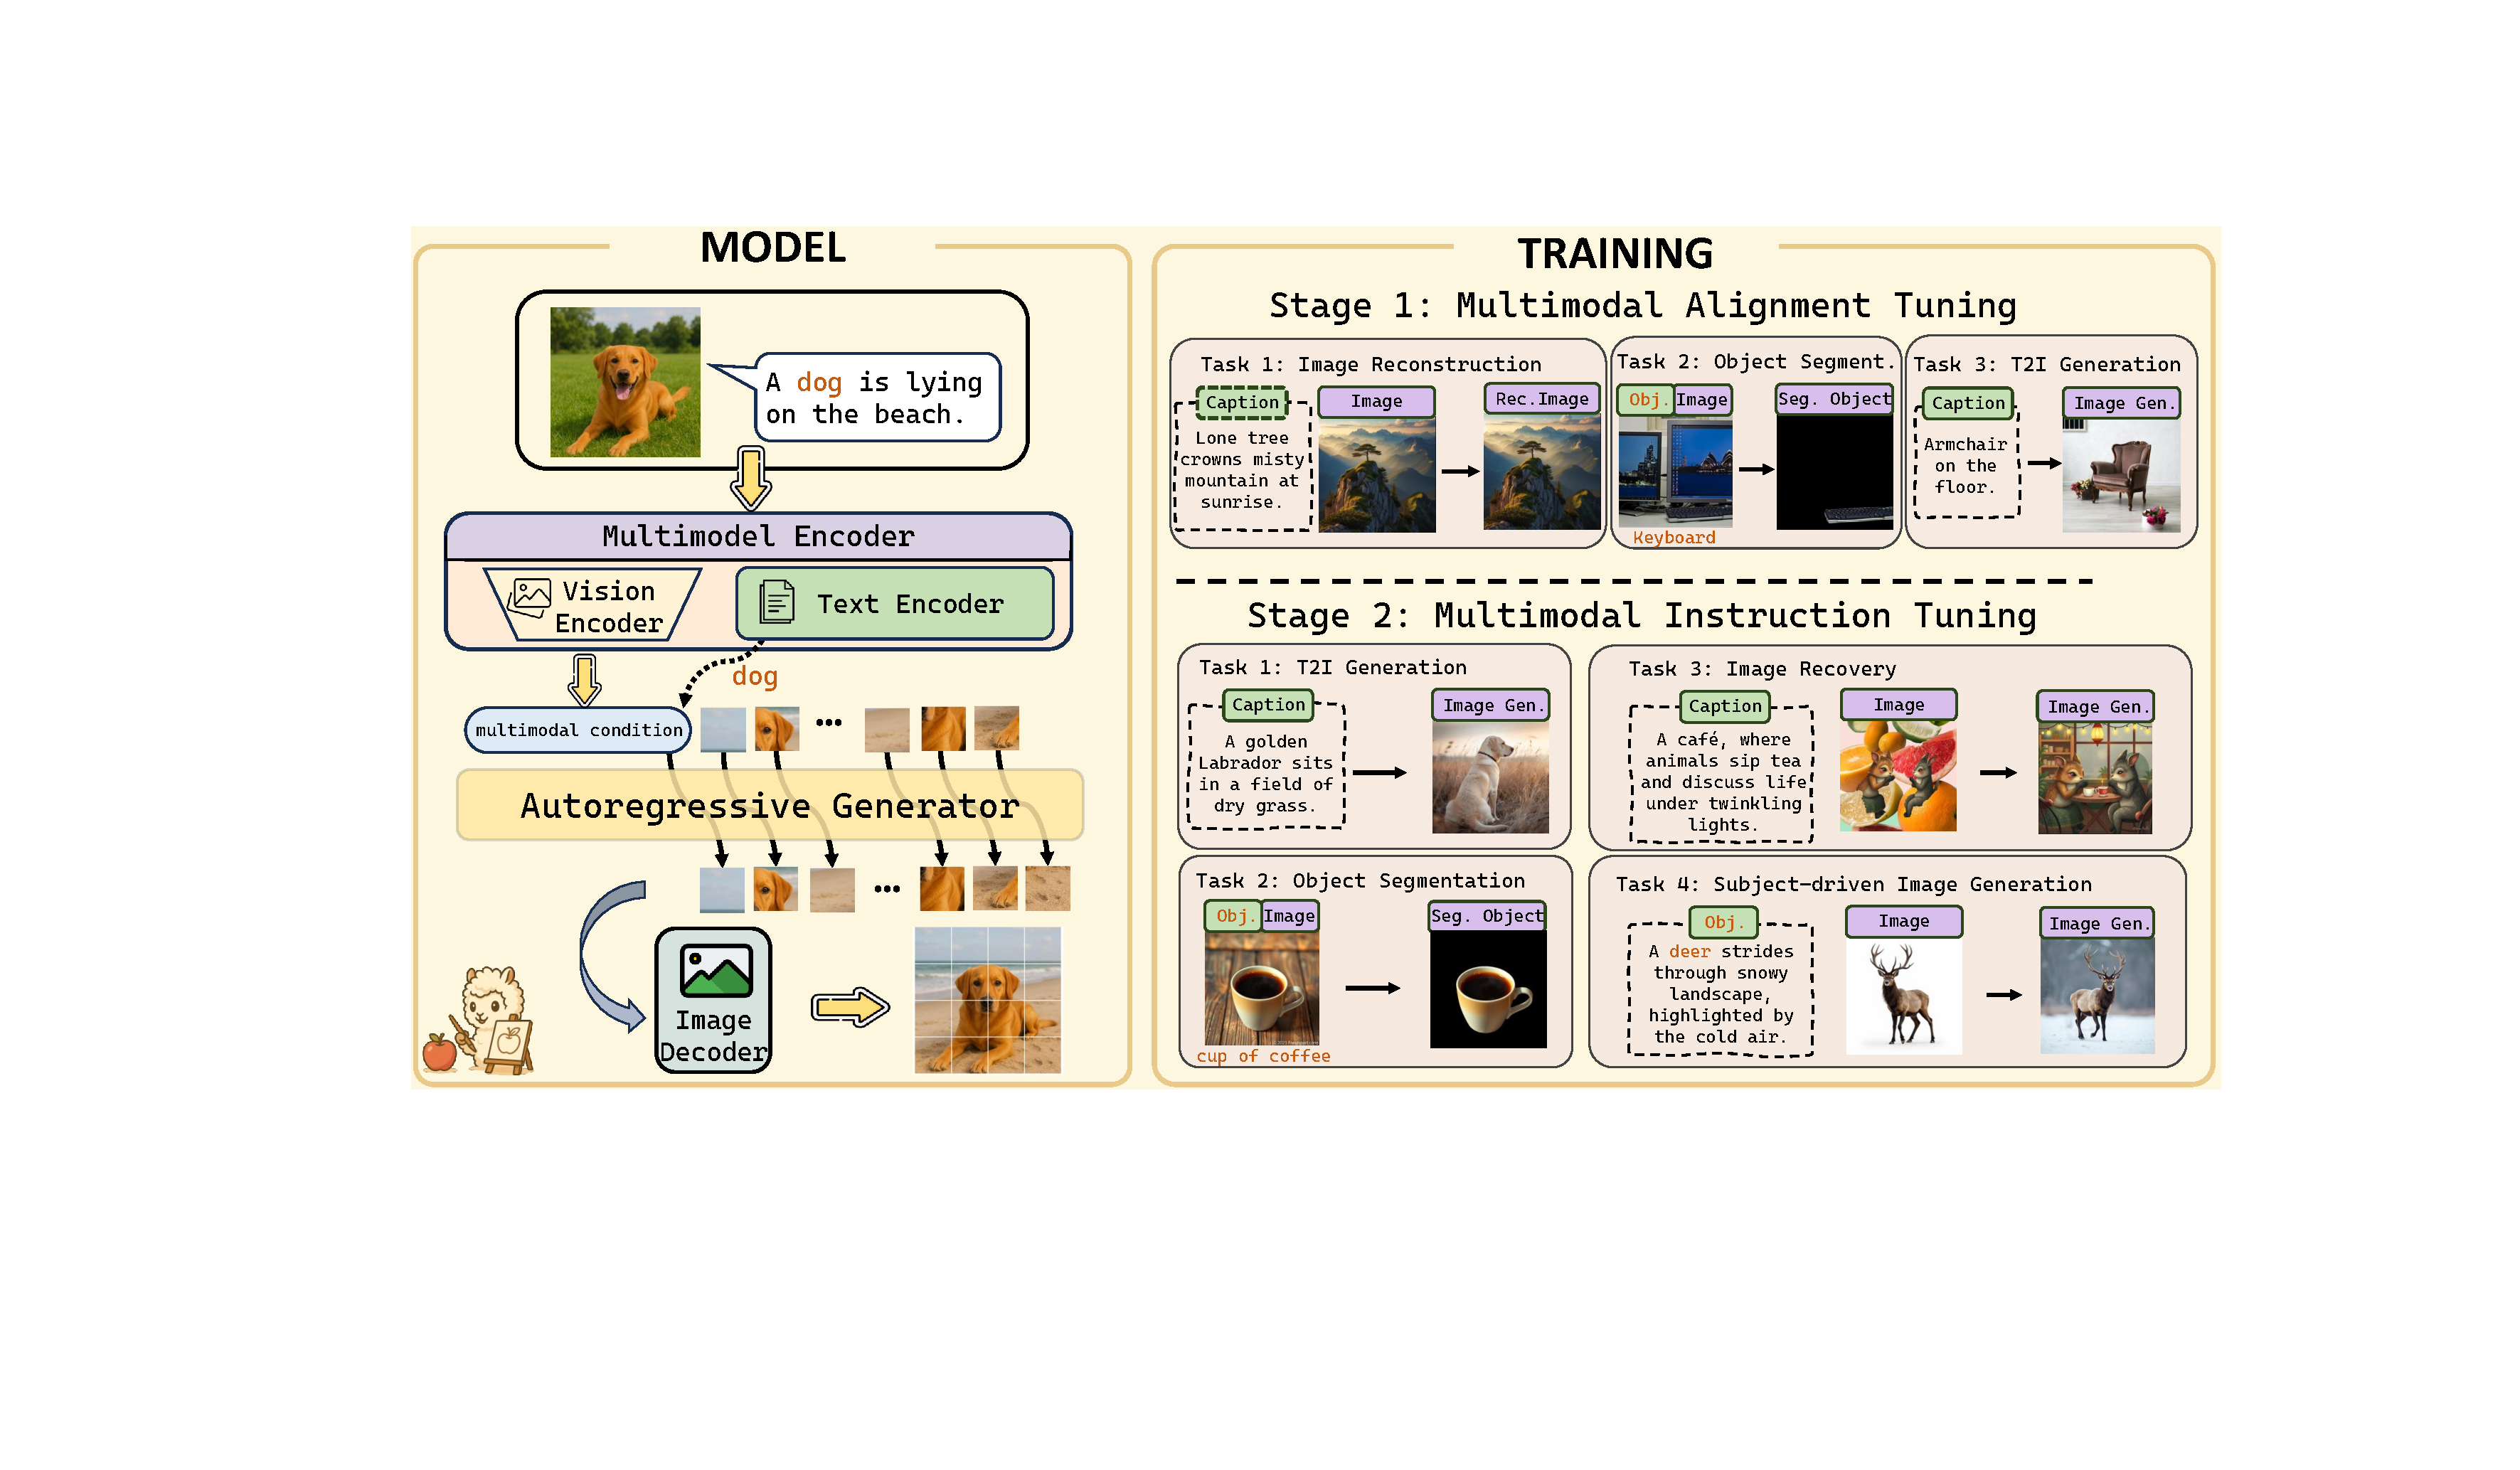
\includegraphics[width=1.0\textwidth]{figures/model_stagev2.pdf}
\caption{Overview of \model. \textbf{Left} panel illustrates the model structure, where visual and textual inputs are encoded into a unified latent to guide autoregressive image generation. \textbf{Right} panel highlights the two-stage training paradigm: (1) \textbf{Multimodal Alignment Tuning}, enabling pixel and semantic-level alignment between inputs and output tokens; and (2) \textbf{Multimodal Instruction Tuning}, compels model to effectively balance influence of different modalities.}
\label{fig:structure}
\vspace{-3ex}
\end{figure*}
\textbf{Autoregressive Generation Decoder}
A transformer-based autoregressive decoder generates a image token sequence $\mathbf{y} = (y_1, \dots, y_{L})$ conditioned on the prefix $\mathbf{H}$ generated by the multimodal encoder and previously generated tokens $y_{<i}$. It operates in a shared embedding space with the encoder's output and shares the same vocabulary as the VQGAN~\citep{Esser2020TamingTF} that is used for image tokenization.
The generated token sequences are subsequently decoded into images using the VQGAN decoder. This unified autoregressive structure facilitates unified training via next-token prediction.

% The decoder, a transformer-based autoregressive model, generates a sequence of image tokens $\mathbf{y} = (y_1, \dots, y_{L})$ conditioned on the prefix $\mathbf{h}$ and previously generated tokens $y_{<i}$. It operates in a shared embedding space with the encoder's output and uses the same discrete token vocabulary as the VQGAN employed for target image tokenization and final image synthesis from $\mathbf{y}$. This structure supports unified training via next-token prediction.

\subsection{Two-Stage Training Paradigm}
\label{sec:traing_stages}
As highlighted in the introduction, effectively aligning disparate modalities and balancing their influence are crucial challenges for multimodal conditional generation. Our carefully designed two-stage training paradigm directly addresses these issues, moving beyond initial coarse alignment to foster robust understanding and balanced integration of diverse inputs, as illustrated in \Cref{fig:structure}. 

\textbf{Stage 1: Multimodal Alignment Tuning}
While the initial connector training provides preliminary semantic alignment, we observed that the model primarily interprets visual inputs semantically like text captions, neglecting crucial visual and spatial details necessary for precise image generation. This stage is dedicated to explicitly enhancing both pixel and semantic-level modality alignment and promoting the utilization of visual information.
In Stage 1, we employ three complementary tasks:
\begin{itemize}[left=2pt, itemsep=0.5pt,topsep=0.5pt]
    \item \emph{\textbf{Image reconstruction}}, where models must faithfully reconstruct an input image conditioned on itself, with the corresponding caption randomly provided or omitted, reinforcing pixel-level fidelity.
    \item \emph{\textbf{Object segmentation}}, where models are given an input image and a target object label and must generate an end‐to‐end segmented figure for that object. This task compels the model to explicitly capture fine-grained visual details and spatial structures associated with specific semantic concepts.
    \item \emph{\textbf{T2I generation}}, using image-caption pairs to preserve and reinforce foundational generative capabilities learned during pretraining of the decoder.
\end{itemize}
Importantly, incorporating the segmentation task alongside image reconstruction mitigates the risk of the model degenerating into a trivial copy-paste behavior, such as simply replicating the input. The segmentation objective compels the model to produce semantically meaningful and spatially precise visual outputs. This complementary effect has been further analyzed and validated in \Cref{abl:stage1}.

% In Stage 1, we employ two complementary pretraining tasks:  

% \begin{itemize}[left=2pt]
% \item \emph{\textbf{image reconstruction}}, where the model must faithfully reconstruct the input image conditioned on itself, reinforcing pixel-level fidelity.
% \item \emph{\textbf{Object segmentation}}: Given an image and a target label, the model outputs an end‑to‑end segmentation of that target, cultivating fine spatial understanding and visual attention essential for visual grounding and controllable image generation.
% \item \emph{\textbf{Text-to-image generation}}: Training with image–caption pairs preserves and refines the model’s capacity to turn textual descriptions into coherent images, ensuring outputs remain firmly grounded in the input text.
% \end{itemize}

% Importantly, employing the segmentation task alongside reconstruction helps prevent from solutions—such as merely copying inputs—by requiring the model to generate semantically meaningful and spatially precise visual outputs based on multimodal conditions.

% While the preliminary alignment phase achieves coarse semantic alignment for the model, we observe that the decoder tends to treat visual inputs as text‐like captions, which predominantly captures semantic-level information, neglecting crucial pixel-level visual details necessary for precise image generation. To address this, we introduce a dedicated first stage of training designed explicitly to enhance both semantic-level and pixel-level modality alignment.

% 需要的宏包
% \usepackage{booktabs}
% \usepackage{siunitx}      % 千位分隔可选
% \sisetup{group-separator = {,}}

% %-------------------------------------------
% \begin{table}[t]
% \small
%   \begin{flushright}              % 靠右
%   \begin{minipage}{0.48\textwidth}% 右半页(≈0.5\textwidth)
%     \centering
%     \caption{Pipeline statistics}
%     \resizebox{\textwidth}{!}{%
%     \begin{tabular}{@{}l S@{}}
%       \toprule
%       \textbf{Category}       & \textbf{Value} \\
%       \midrule
%       Total                   & 3\,058\,356 \\[2pt]

%       \textbf{Stage 1}        & \textbf{2\,494\,674} \\
%       \quad t2i               & 7\,000\,000 \\
%       \quad segment           & 1\,614\,674 \\
%       \quad recover           &   180\,000 \\[2pt]

%       \textbf{Stage 2}        & \textbf{1\,313\,682} \\
%       \quad t2i               &   600\,000 \\
%       \quad segment           &   150\,000 \\
%       \quad recover           &   150\,000 \\
%       \quad subject-driven    &   413\,682 \\
%       \bottomrule
%     \end{tabular}}
%   \end{minipage}
%   \end{flushright}
% \end{table}
%-------------------------------------------


% \begin{figure*}[htbp]
%     \centering
%     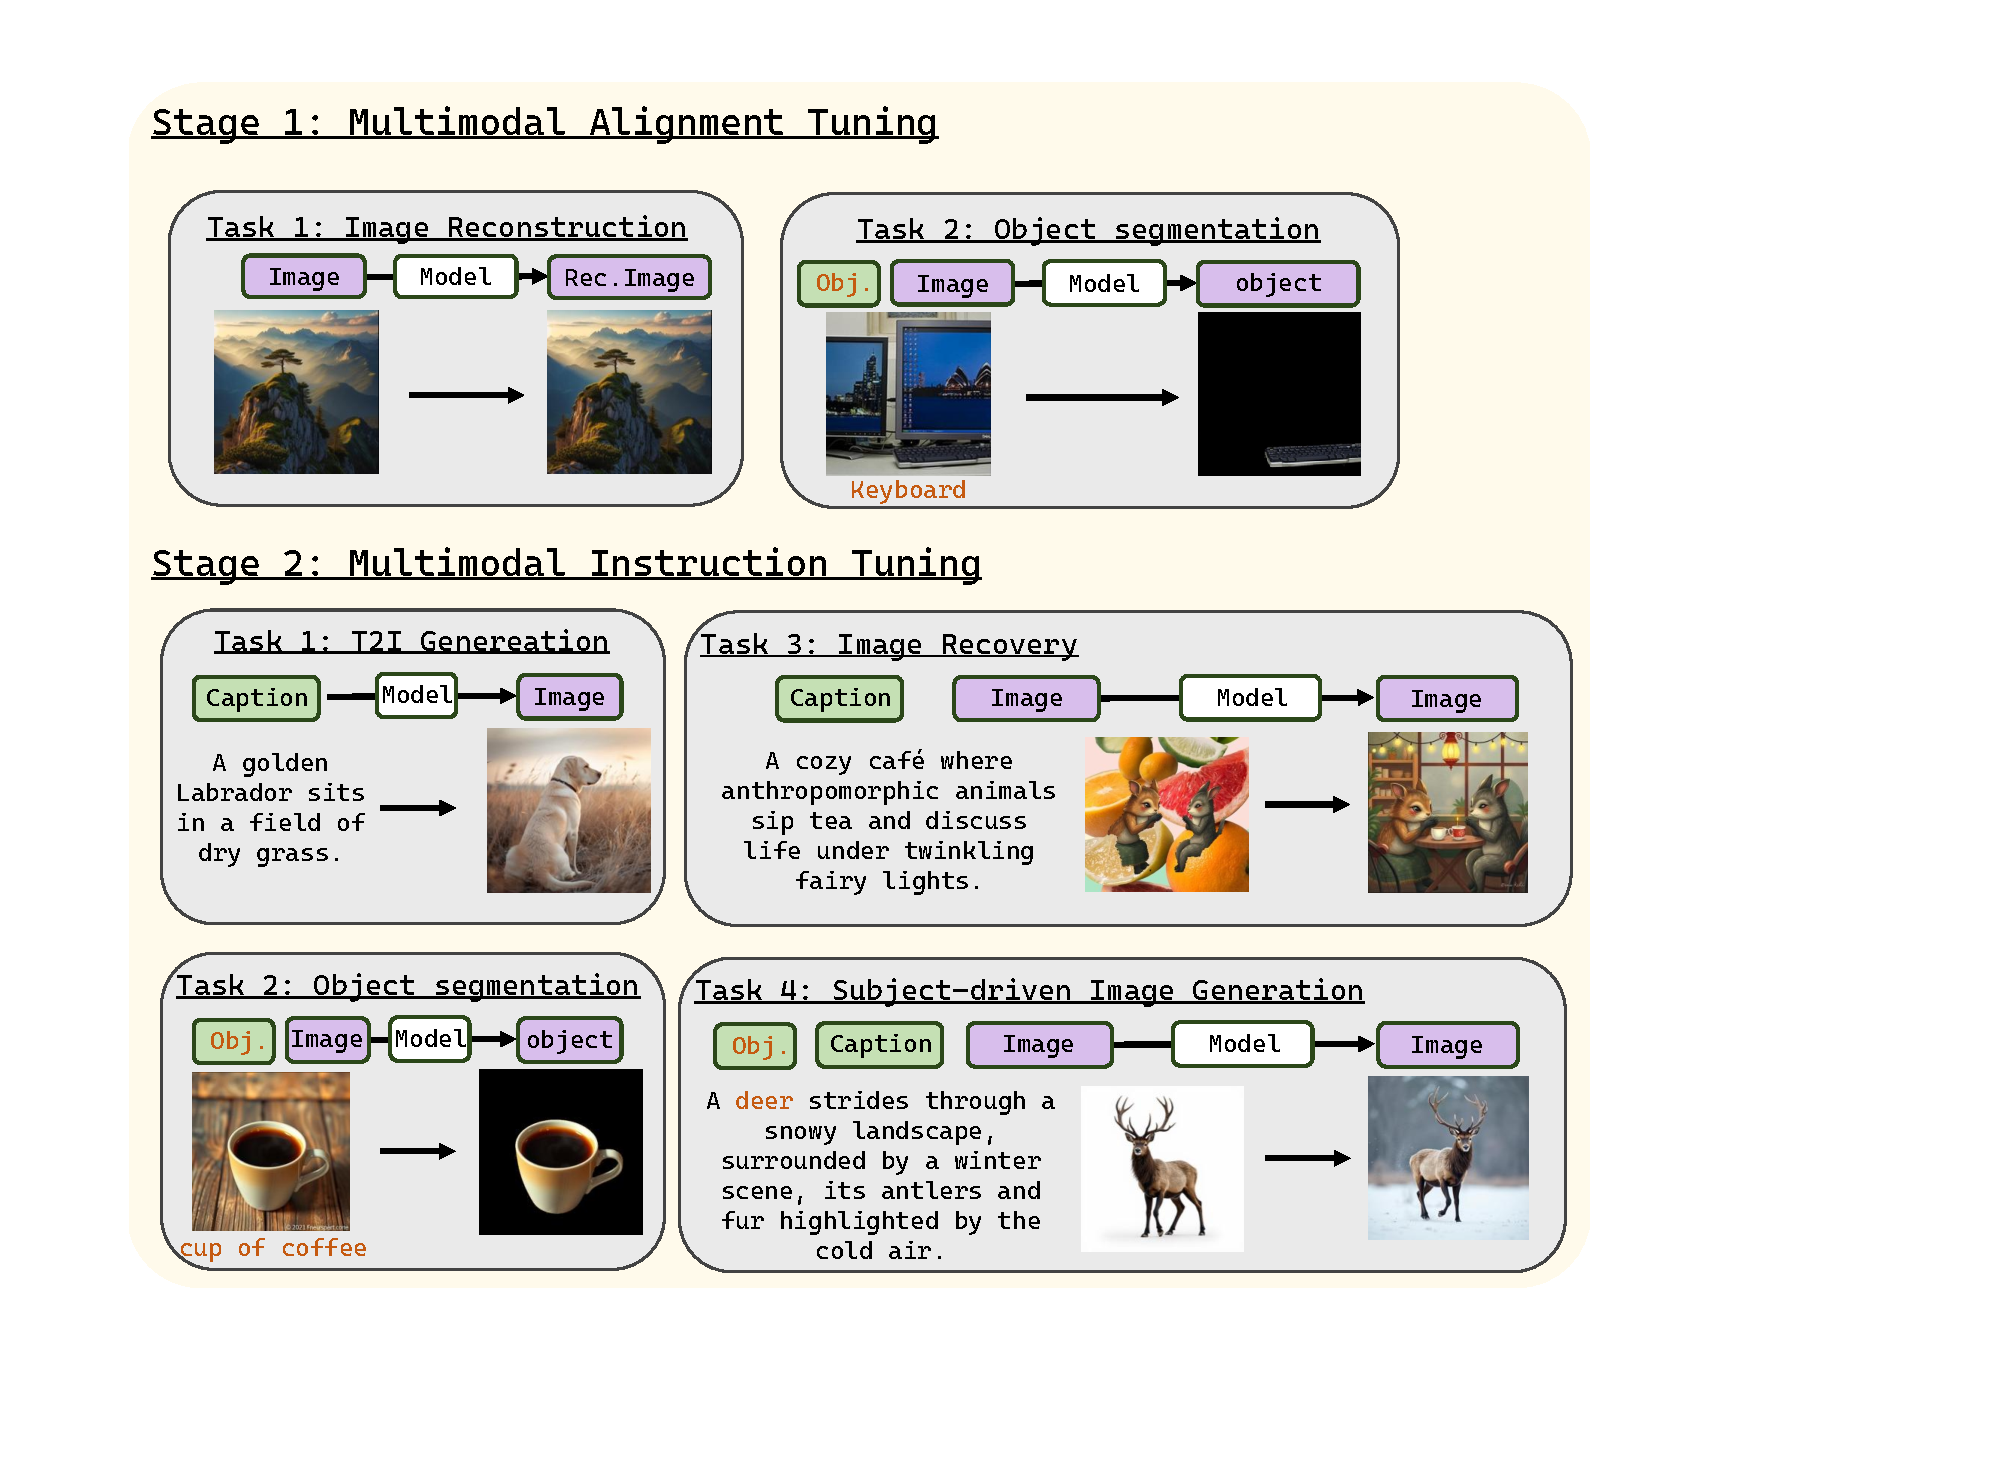
\includegraphics[width=1.0\textwidth]{figures/stages.pdf} 
%     \caption{Training Stage Placeholder
%     }
%     \label{fig:structure}
% \end{figure*}





% \begin{itemize}[left=2pt]
%     \item \emph{\textbf{Image reconstruction}}, where the model must faithfully reconstruct the input image conditioned on itself, reinforcing pixel-level fidelity.
%     \item \emph{\textbf{Object segmentation}}, where the model is given an input image and a target object label and must generate an end‐to‐end segmented figure for that object. This task compels the model to explicitly capture fine-grained visual details and spatial structures associated with specific semantic concepts.
%     \item \emph{\textbf{Text-to-image generation}}, using image-caption pairs to preserve and reinforce foundational generative capabilities learned during pretraining of the decoder.
% \end{itemize}
% Importantly, employing the segmentation task alongside reconstruction helps prevent trivial solutions—such as merely copying inputs—by requiring the model to generate semantically meaningful and spatially precise visual outputs based on the provided conditions.
% e visual outputs based on the provided conditions.


% \item \emph{\textbf{text-to-image generation}} training using image-caption pairs to preserve and reinforce foundational generative capabilities learned during pretraining of the decoder.
% \item \emph{\textbf{object segmentation}}, where the model is given an input image and a target object label and must generate an end‐to‐end segmented figure for that object. It further compels the model to explicitly capture fine-grained visual details and spatial structures associated with specific semantic concepts.
% (i)  \emph{image reconstruction}, where the model must faithfully reconstruct the input image conditioned on itself, reinforcing pixel-level fidelity; and (ii) \emph{object segmentation}, where the model is given an input image and a target object label and must generate an end‐to‐end segmented figure for that object. It further compels the model to explicitly capture fine-grained visual details and spatial structures associated with specific semantic concepts.
% Additionally, we integrate standard text-to-image generation training using image-caption pairs to preserve and reinforce foundational generative capabilities learned during pretraining of the decoder.
% Importantly, employing the segmentation task alongside reconstruction helps prevent from solutions—such as merely copying inputs—by requiring the model to generate semantically meaningful and spatially precise visual outputs based on multimodal conditions.

% Importantly, employing the segmentation task alongside reconstruction helps prevents shortcut solutions—such as directly copying inputs—by compelling the model to focus on semantically meaningful yet spatially precise visual information. Additionally, we integrate standard text-to-image generation training using image-caption pairs to preserve and reinforce foundational generative capabilities.







% The second stage of training is designed to address a central challenge in multimodal generation: ensuring the model can jointly attend to and integrate diverse input modalities in a balanced and controllable manner. 
% While the first stage focuses on aligning modalities and reinforcing the visual fidelity, Stage 2 aims to endow the model with the instruction-following ability and cross-modal reasoning capacity necessary for robust and nuanced image generation.
% Beside object segmentation and text-to-image generation, we use two additional tasks.
% To this end we adopt the multimodal instruction tuning with carefully–chosen training task. Training samples are drawn from a mixture of four complementary tasks, each targeting a distinct aspect of multimodal image generation:
% This is achieved through instruction tuning with diverse tasks designed to encourage comprehensive multimodal proficiency:

% The second stage targets enhancing the model’s capacity to jointly leverage multimodal conditions effectively during image generation, emphasizing balanced integration across modalities. 
% Specifically, we design this stage around four core training tasks to ensure comprehensive multimodal proficiency:
% \begin{itemize}[left=2pt]
% \item \emph{\textbf{Image recovery}}: Synthetically augmenting data by rotating, resizing, and compositing segmented object masks onto random backgrounds paired with original captions. This process requires the model to reconstruct the full original image, compelling it to effectively extract and integrate essential visual details from distorted contexts while relying on textual instructions to infer and restore missing components. It compels the model to fuse noisy or incomplete visual cues with textual guidance, promoting robust multimodal inference and error correction.
% \item \emph{\textbf{Subject-driven image generation}}: Conditioning on both reference images and textual instructions to serve as a final end-to-end task, fully exercising cross-modal fusion.
% \end{itemize}

% This balanced, multi-task instruction tuning ensures that the model learns to implicitly attend to and integrate both visual and textual signals harmoniously, preventing over-reliance on any single modality and yielding precise, controllable multimodal conditional generation.

\textbf{Stage 2: Multimodal Instruction Tuning}
Stage 2 aims to endow the model with robust instruction-following and cross-modal reasoning capabilities for nuanced and controllable multimodal generation, building upon the alignment and visual fidelity established in Stage 1. The model is expected to jointly attend to and integrate diverse input modalities in a balanced and controllable manner.
To achieve this, we employ a multimodal instruction tuning strategy based on a carefully curated mixture of training tasks. Specifically, we reuse the \emph{\textbf{T2I generation}} and \emph{\textbf{object segmentation}} tasks from Stage 1, maintaining identical data and formulations. These tasks respectively reinforce the model’s ability to adhere to and utilize textual and visual modalities, helping preserve foundational skills and stabilize the training process.
In addition, we introduce two novel tasks specifically designed to enhance instruction adherence and foster a balanced integration of multimodal inputs, preventing the model from over-emphasizing a single modality while neglecting others:
\begin{itemize}[left=2pt, itemsep=0.5pt,topsep=0.5pt]
    \item \emph{\textbf{Image recovery}}, where we synthetically distort images by rotating, resizing, and compositing segmented objects onto random backgrounds, then pair synthetic images with their original captions to create inputs. The model is then required to reconstruct the original image from the distorted input and corresponding caption. 
    It compels the model to extract and integrate essential visual details from noisy or incomplete visual inputs while leveraging textual cues to infer and restore missing components, promoting robust multimodal reasoning and error-correction performance.
    \item \emph{\textbf{Subject-driven image generation}}, where the model is conditioned on reference image, subject label and textual instruction to generate images. 
    It require the model to actively preserve the subject’s visual identity from the reference image while strictly adhering to the textual instructions for image generation. This task serves as a comprehensive end-to-end objective, fully exercising model’s cross-modal fusion and instruction-following abilities.
\end{itemize}
Overall, this training strategy—combining continued refinement of core capabilities with targeted instruction-based tasks—ensures the model to learn to integrate visual and textual information in a harmonious and controllable way. It mitigates over-reliance on certain modality and enables precise, controllable multimodal conditional generation, which are further discussed in \Cref{abl:stage2}. 

% \begin{figure*}[htbp]
%     \centering
%     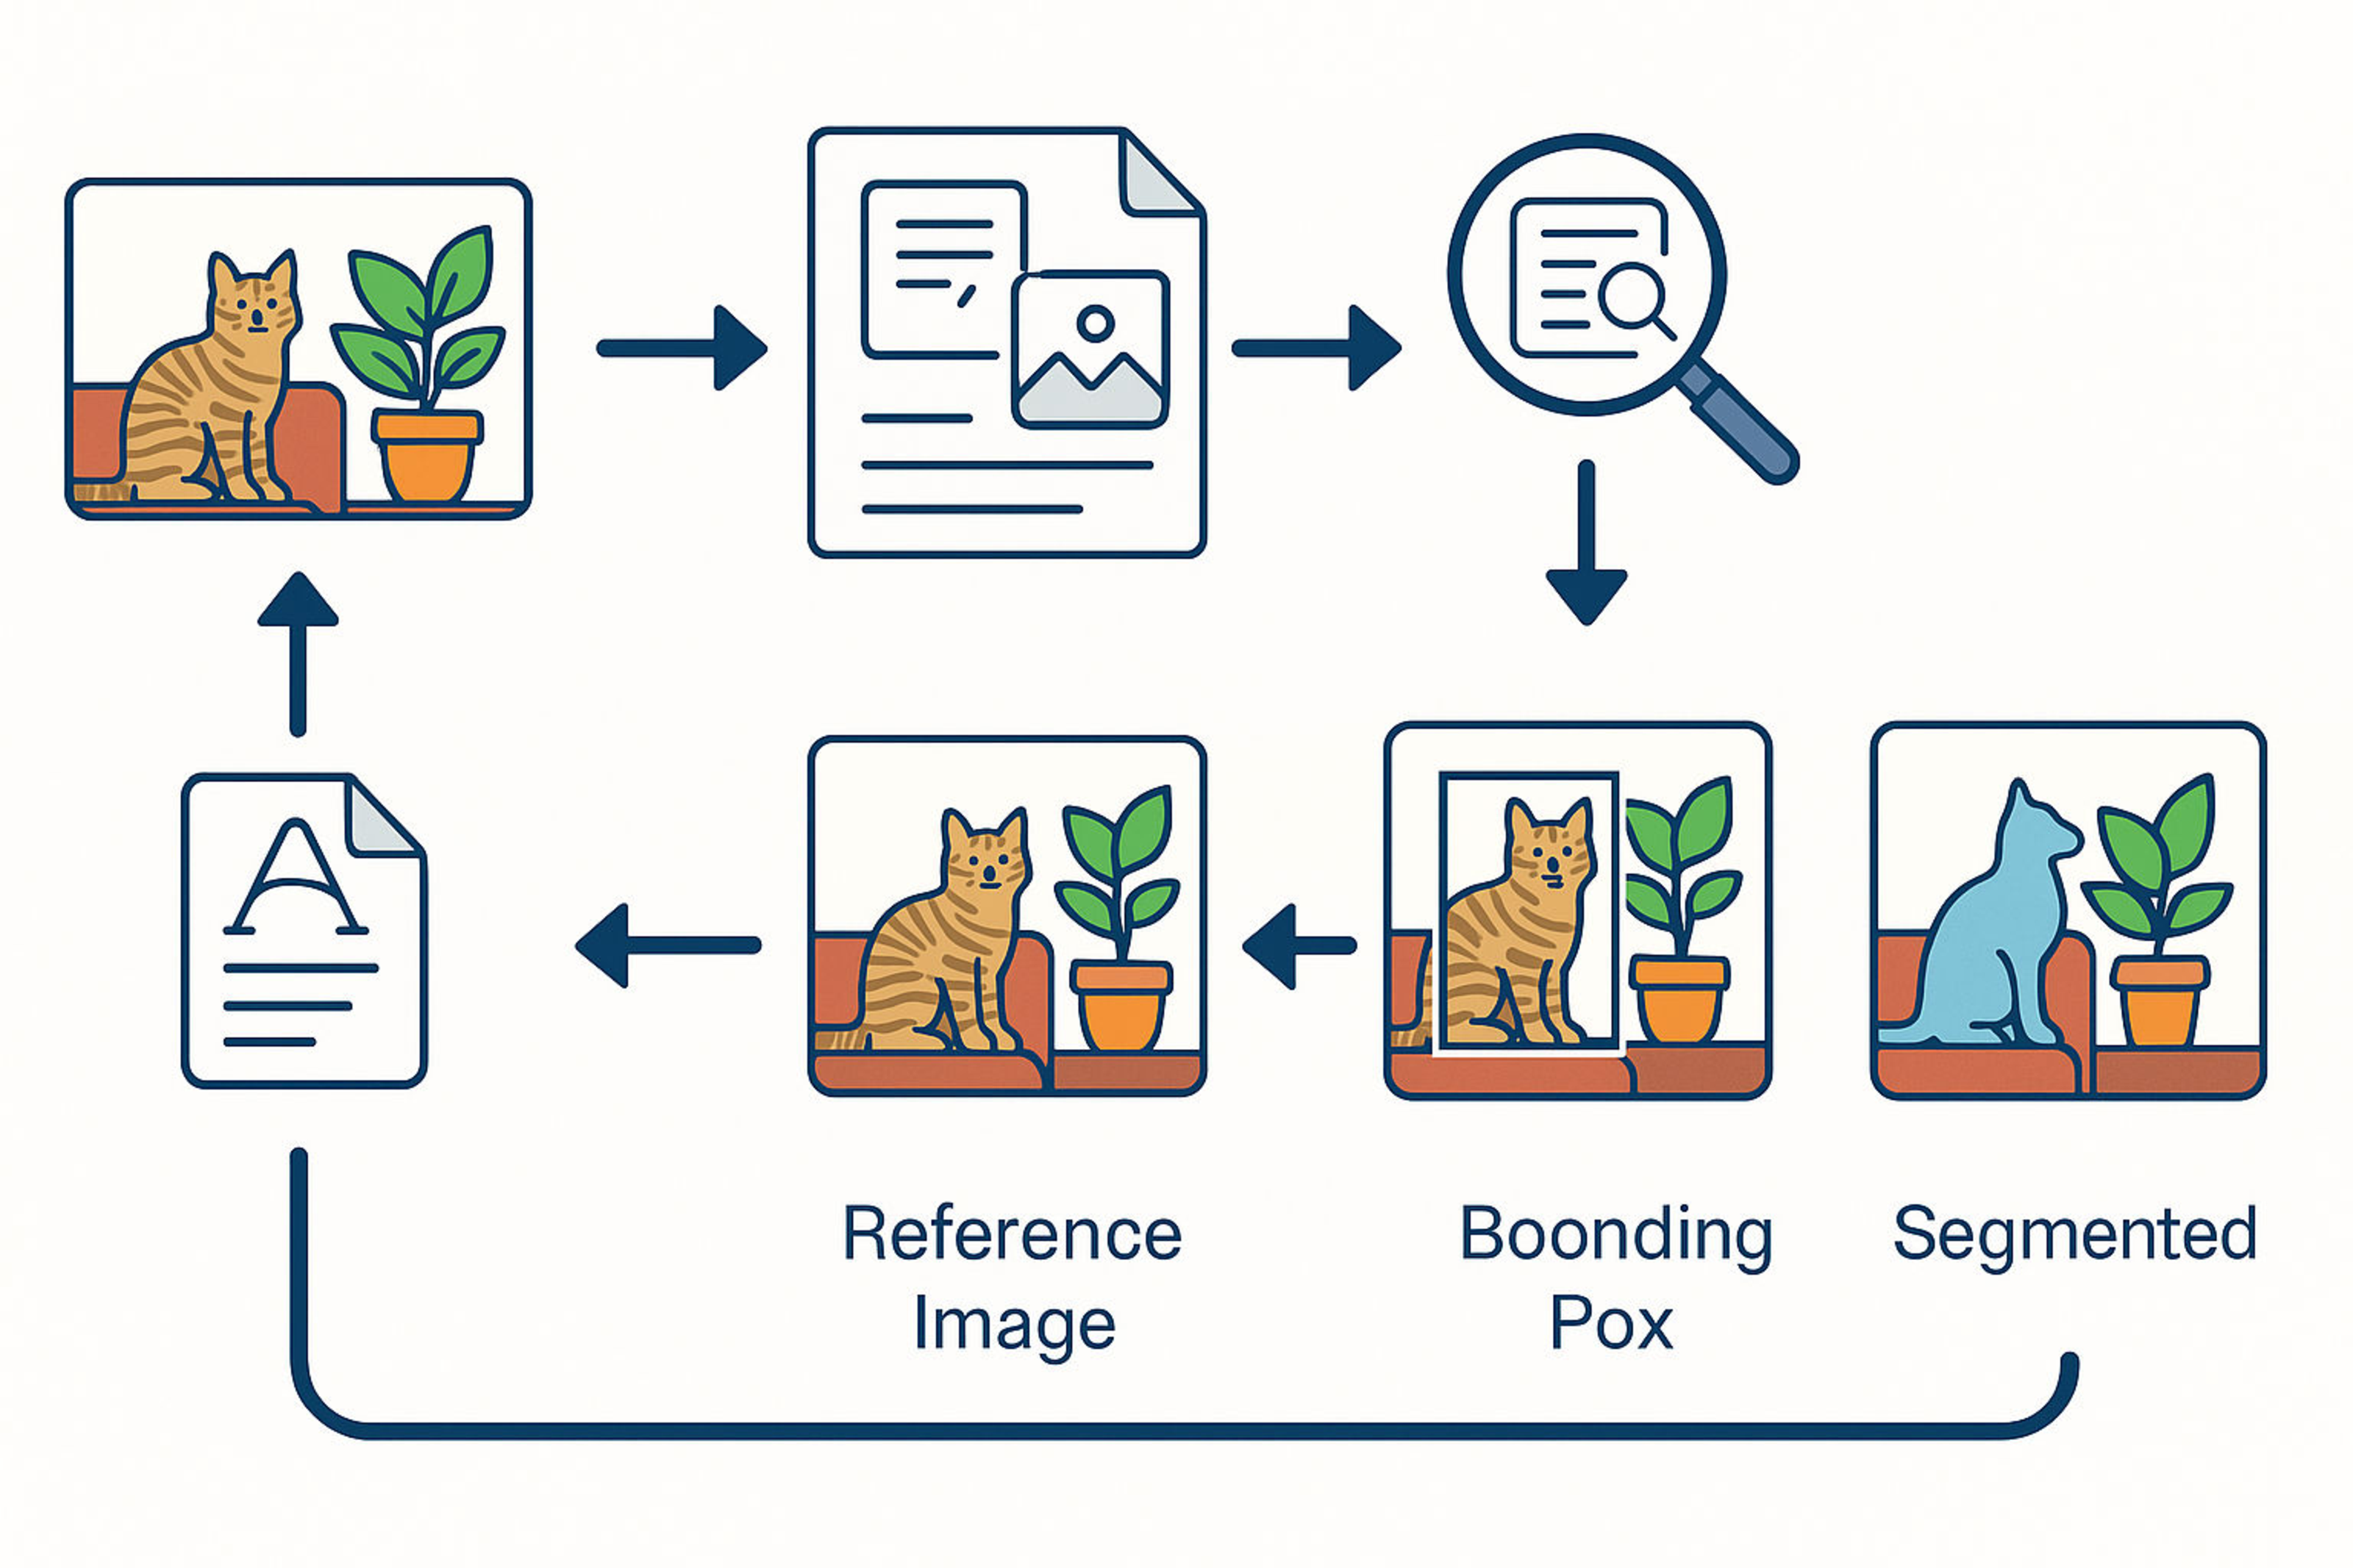
\includegraphics[width=0.8\textwidth]{figures/segment.pdf} 
%     \caption{Data construction pipeline Placeholder
%     }
%     \label{fig:structure}
% \end{figure*}


\subsection{Data Construction}
\label{sec:data_construct}

To support our two-stage training paradigm, we construct a large-scale multimodal dataset comprising approximately \textbf{3 million samples} across all training tasks. It integrates open-source resources, synthetic data, and automated annotations to ensure scalability, diversity, and strong task alignment.
For \textbf{image reconstruction} and \textbf{T2I generation}, we collect image-text pairs from datasets like CC12M~\citep{changpinyo2021cc12m} and Midjourney-Niji~\citep{midjourney-niji-1m-llavanext}.  To broaden domain coverage (e.g., human subjects, artistic scenes), we generate additional samples using T2I models like Flux.1~\citep{flux} and Stable Diffusion v3.5~\citep{2024SD3}, with prompts generated by advanced LLMs~\citep{gpt4o} to enhance semantic and visual diversity.
For \textbf{segmentation} and \textbf{image recovery}, which require fine-grained object-level annotations, we design an automated pipeline that combines state-of-the-art LMMs~\citep{Qwen2vl} with segmentation models\citep{sam}. Given an image, LMMs are queried to produce a comprehensive caption and extract a list of concrete, segmentable objects. For each object, LMMs predicts its spatial location, providing a bounding box and a set of 2D keypoints, which guide the segmentation model in producing high-quality, semantically consistent masks.
For \textbf{subject-driven image generation}, we leverage the OminiControl dataset~\citep{OminiControl}, re-captioned using LMMs to accurately extract subject-relevant descriptions. Additionally, we reverse image pairs to effectively double the usable data.
% The resulting dataset supports a wide range of multimodal tasks, including image reconstruction, T2I generation, object segmentation, and image recovery.
Data construction and formation are detailed in \Cref{sec:data_const}.




% To enable large-scale training, we design an automated pipeline that generates high-quality multimodal training data by combining open-source image datasets with the state-of-the-art vision–language models (VLMs) and segmentation models. This pipeline allows us to construct richly annotated image–text pairs containing multiple segmented foreground objects, without requiring manual labeling.

% The pipeline begins by querying a VLM to generate detailed captions and extract concrete object categories based on the image and generated caption. For each input image, we prompt the model to (1) generate a comprehensive caption that describes all visible, prominent, and foreground elements, and (2) extract a list of distinct, segmentable object names that are tangible and visually present in the image. This step ensures that only concrete and semantically meaningful visual elements are retained for downstream segmentation.

% Given the extracted object list, we then prompt the VLM again—once per object—to identify its spatial location within the image. Specifically, the model is asked to return both a tight bounding box and several representative 2D keypoints for each object. These spatial cues serve two critical roles: they constrain the region of interest for segmentation, and they reduce the likelihood of including irrelevant or overlapping background content. 

% Finally, we employ a high-performance segmentation model to extract object masks from the image, using the generated bounding boxes and keypoints. It eventually produces high-quality masks that are both semantically aligned and spatially accurate.

% By applying this pipeline to a large corpus of open-source images, we construct a multimodal dataset comprising captioned images annotated with multiple precisely segmented objects, which forms a key component of our training setup.



% % \section{Experiments}
\label{sec:experiments}

\subsection{Experimental Setup}
\label{sec:details}

% \textbf{Dataset Formation} 
% Approximately 3 million samples are used: Stage 1 comprises around 2.5 million, and Stage 2 has 1.3 million, with 800K overlapping. Data comes from a mix of open-source datasets like Midjourney~\citep{midjourney-niji-1m-llavanext} and CC12M~\citep{changpinyo2021cc12m}, and synthetic data created with publicly available T2I models, including Flux.1 dev~\citep{flux} and Stable Diffusion v3.5 Large~\citep{2024SD3}. More details are in \Cref{app:data_form} and \Cref{tab:dataset}.


\textbf{Implementation Details} 
The multimodal encoder is initialized using CLIP-Large-Patch14~\citep{Radford2021LearningTV} and Flant5-XL~\citep{flant5}, with a 224×224 image receptive field. 
The generator is initialized from LlamaGen-XL~\citep{llamagen}(775M). A two-layer MLP serves as the projector.
We freeze the encoder, training only the projector and generator for one epoch in Stage 1, then fine-tune the full model (except the vision encoder) for two more epochs in Stage 2.
Training on 8 A100 GPUs (80 GB each) takes about 1.5 days. More details are in \Cref{sec:Exp_Details}.
% To implement the MLP-based Projection, we train the MLP Projector on LLaVA-CC3M-Pretrain-595K data~\citep{liu2023llava}, keeping the vision and text encode frozen following the setting of LLAVA alignment training. For the Query-based Token Distillation, the model is initialized with BLIP2-Flant5-XL~\citep{li2023blip2}.

% \paragraph{Training Details}
% \label{sec:setup}


% To further investigate the effect of multi-image conditioning in multimodal generation, we continue training the model using a mixture of Stage 2 data and additional multi-subject samples generated via our data construction pipeline. In this setting, the model is tasked with reconstructing the original image based on segmented object crops and the corresponding image caption. Training is conducted for one additional epoch with a learning rate of 5e-5. Due to context length constraints, we limit each example to a maximum of three sub-images, resulting in a total sequence length of 888 tokens.

% \subsection{Evaluation Setup}


\textbf{Benchmark \& Metric.} We evaluate \model on \textbf{DreamBench}~\citep{ruiz2023dreamboothfinetuningtexttoimage} and \textbf{DreamBench\texttt{++}}~\citep{peng2025dreambenchpp} benchmarks.
\textbf{DreamBench} employs CLIP and DINO scores to measure the fidelity to images and prompts.
\textbf{DreamBench\texttt{++}} offers a scaled and diverse evaluation dataset and introduces a human-aligned automatic evaluation protocol using GPT-4o, addressing limitations of DreamBench evaluation.
GPT-4o evaluator scores generations on two axes: \textbf{Concept Preservation (CP)}, measuring the retention of the subject's visual identity, and \textbf{Prompt Following (PF)}, evaluating how accurately the image reflects the text prompt.
% Performance on DreamBench\texttt{++} is summarized by the combined CP$\cdotp$PF score, reflecting a balanced overall generation capability.
Details can be found in the \Cref{app:DreamBench_Plus}.

% \textbf{DreamBench} includes 30 subjects and 25 prompts, evaluating subject-driven generation via image–image and image–text similarity. It uses CLIP and DINO embeddings to compute subject fidelity (between the generated and reference image) and prompt fidelity (between the generated image and the prompt).

% \textbf{DreamBench\texttt{++}} significantly scales up the evaluation with 150 subjects and 1,350 prompts spanning photorealistic, stylistic, and imaginative settings. It uses GPT-4o as an automatic evaluator, scoring each image on two axes:

% \begin{itemize}
%     \item \textbf{Concept Preservation (CP):} Measures how well the generated image retains the visual identity of the reference subject (e.g., shape, color, texture, and facial details).
%     \item \textbf{Prompt Following (PF):} Evaluates how accurately the image reflects the semantics and context of the text prompt, including relevance, accuracy, and completeness.
% \end{itemize}


\textbf{Baselines.}
We compare our method against various baselines, categorized as follows:
\begin{itemize}[left=2pt, itemsep=0.5pt,topsep=0.5pt]
    \item \textbf{Fine-tuning-based methods:} Textual Inversion~\citep{gal2022imageworthwordpersonalizing}, and DreamBooth~\citep{peng2025dreambenchpp}, which fine-tune models with auxiliary control mechanisms on a subset of benchmark data.
    \item \textbf{Test Time Tuning-Free Methods:} Models pretrained on large-scale data and evaluated in a zero-shot. Diffusion-based models like BLIP-Diffusion~\citep{li2023blipdiffusionpretrainedsubjectrepresentation}, Emu2~\citep{emu2}, variants of IP-Adapter~\citep{ye2023ip-adapter}, and DreamEngine~\citep{dreamengine}, as well as autoregressive models like Unified-IO 2~\citep{lu2023unifiedio2} and Lumina-mGPT~\citep{2024lumina}. 
\end{itemize}

% \textbf{Baselines.} We compare our method against a range of baselines, categorized as follows:

% \noindent\makebox[2pt][l]{•}~\textbf{Fine-tuning-based methods.} Textual Inversion~\citep{gal2022imageworthwordpersonalizing} and DreamBooth~\citep{peng2025dreambenchpp}, which fine-tune models with auxiliary control mechanisms on subsets of benchmark data.

% \noindent\makebox[2pt][l]{•}~\textbf{Test-time tuning-free methods.} These models are pretrained on large-scale multimodal data and evaluated in a zero-shot setting without subject-specific fine-tuning. This category includes diffusion-based models such as BLIP-Diffusion~\citep{li2023blipdiffusionpretrainedsubjectrepresentation}, Emu2~\citep{emu2}, variants of IP-Adapter~\citep{ye2023ip-adapter}, and DreamEngine~\citep{dreamengine}, as well as autoregressive models like Unified-IO 2~\citep{lu2023unifiedio2} and Lumina-mGPT~\citep{2024lumina}.



\subsection{Main results}
\label{sec:main}
\Cref{tab:comparison} comprehensively evaluates our proposed autoregressive (AR) framework on the DreamBench++ benchmark, comparing it with diffusion-based and autoregressive-based baselines.
\model demonstrates highly competitive performance, particularly in achieving a strong balance between the guidance of both input modalities. Notably, this is achieved despite utilizing significantly fewer training resources and suboptimal model components compared to the state-of-the-art baselines.
% We assess performance along two key axes: Concept Preservation (CP)—measuring fidelity to the reference subject—and Prompt Following (PF)—evaluating semantic alignment with the textual prompt.

\textbf{Overall Performance.}
\model achieves a strong balance between concept fidelity and prompt alignment, resulting in the high \textbf{CP$\cdotp$PF} score. 
% Notably, even without task-specific fine-tuning and using a modest model size and training data, 
\model rivals fine-tuned methods like DreamBooth-LoRA, while significantly outperforming test-time tuning-free baselines such as Emu2 and DreamEngine. For instance, \model surpasses Emu2 in CP$\cdotp$PF score by approximately 30\%. 
% While fine-tuning methods like DreamBooth LoRA (0.52) achieve a higher CP$\cdotp$PF score, they benefit from training directly on the test set subjects, whereas our method operates in a test-time tuning-free manner.
A key strength of \model is its ability to harmoniously integrate multimodal inputs. Several strong baselines, including some AR methods like Lumina-mGPT and Unified-IO2, exhibit very high Concept Preservation (CP) but suffer from extremely low Prompt Following (PF), resulting in high \textbf{CP/PF} scores. This indicates a tendency to over-rely on the reference image while neglecting textual instructions. In contrast, \model delivers lowest CP/PF scores compared to all test-time tuning-free baselines, demonstrating effective and controlled integration of both visual and textual guidance.


\begin{table}[t]
\vspace{-8ex}
\centering
\small
\caption{
Comparison on DreamBench++. Models are ranked by \textbf{CP$\cdotp$PF}, indicating balanced overall multimodal image generation performance. \textbf{CP/PF} ratio reflects overfitting issue toward certain modality. ``*'' denotes model trained \textbf{from scratch}; others are adapted from pre-trained T2I models.
}

\label{tab:comparison}
\resizebox{\textwidth}{!}{%
\begin{tabular}{@{}l@{\hspace{1ex}}c@{\hspace{1ex}}c@{\hspace{1ex}}c@{\hspace{1ex}}c@{\hspace{1ex}}c@{\hspace{1ex}}c@{\hspace{1ex}}c@{\hspace{1ex}}c@{\hspace{1ex}}c@{\hspace{1ex}}c@{\hspace{1ex}}c@{\hspace{1ex}}c@{\hspace{1ex}}c@{\hspace{1ex}}c@{}}
\toprule
\textbf{Method} & \textbf{T2I Model} & \textbf{Train Data} & \textbf{Model Size} 
& \multicolumn{5}{c}{\textbf{Concept Preservation (CP)}} 
& \multicolumn{4}{c}{\textbf{Prompt Following (PF)}} 
& \textbf{CP$\cdotp$PF} & \textbf{CP/PF} \\
\cmidrule(lr){5-9} \cmidrule(lr){10-13}
& & & & \textbf{Animal} & \textbf{Human} & \textbf{Object} & \textbf{Style} & \textbf{Overall} 
& \textbf{Photo.} & \textbf{Style.} & \textbf{Imag.} & \textbf{Overall} & & \\
\midrule
\multicolumn{15}{c}{\textbf{Finetuned on Test Set}} \\
\midrule
Textual Inv.         & SD v1.5      & -     & 860M    & 0.50 & 0.36 & 0.31 & 0.36 & 0.38 & 0.67 & 0.69 & 0.44 & 0.62 & 0.24 & 0.61 \\
DreamBooth           & SD v1.5      & -     & 860M    & 0.64 & 0.20 & 0.49 & 0.48 & 0.49 & 0.79 & 0.78 & 0.50 & 0.72 & 0.36 & 0.68 \\
DreamBooth-L         & SDXL v1.0    & -     & 2.60B   & 0.75 & 0.31 & 0.54 & 0.72 & 0.60 & 0.90 & 0.90 & 0.75 & 0.87 & 0.52 & 0.69 \\

\midrule
\multicolumn{15}{c}{\textbf{Test-Time Tuning-Free Methods}} \\
\midrule
Unified-IO2*         & Unified-IO2  & 8.5B    & 7.00B   & 0.77 & 0.80 & 0.64 & 0.82 & 0.72 & 0.24 & 0.18 & 0.11 & 0.19 & 0.14 & 3.79 \\
Lumina-mGPT          & Chameleon    & 10M     & 7.00B   & 0.95 & 0.97 & 0.89 & 0.85 & 0.91 & 0.31 & 0.25 & 0.15 & 0.25 & 0.23 & 3.64 \\

DreamEngine          & SD3.5        & 21M     & 10.50B  & 0.76 & 0.72 & 0.61 & 0.73 & 0.68 & 0.44 & 0.37 & 0.25 & 0.37 & 0.26 & 1.84 \\

BLIP-Diffusion       & SD v1.5      & 130M    & 1.56B   & 0.67 & 0.56 & 0.47 & 0.51 & 0.55 & 0.58 & 0.51 & 0.30 & 0.50 & 0.27 & 1.10 \\

Kosmos-G             & SD v1.5      & 200M    & 3.00B   & 0.62 & 0.63 & 0.46 & 0.57 & 0.54 & 0.48 & 0.62 & 0.41 & 0.51 & 0.28 & 1.06 \\

IP-A-Plus ViT-H      & SDXL v1.0    & 10M     & 3.00B   & 0.90 & 0.85 & 0.76 & 0.91 & 0.83 & 0.50 & 0.38 & 0.28 & 0.41 & 0.34 & 2.02 \\

Emu2                 & SDXL v1.0    & 16M     & 37.00B  & 0.67 & 0.55 & 0.45 & 0.45 & 0.53 & 0.73 & 0.72 & 0.56 & 0.69 & 0.36 & 0.77 \\

IP-A ViT-G           & SDXL v1.0    & 10M     & 2.50B   & 0.67 & 0.56 & 0.50 & 0.75 & 0.59 & 0.74 & 0.63 & 0.45 & 0.64 & 0.38 & 0.92 \\
\rowcolor{gray!20} \model & LlamaGen & 3M      & 2.31B   & 0.65 & 0.36 & 0.57 & 0.47 & 0.55 & 0.86 & 0.85 & 0.80 & 0.84 & \textbf{0.47} & \textbf{0.65} \\
\bottomrule
\end{tabular}%
}
\end{table}



% Importantly, despite relying on a relatively low-quality image generator and sub-optimal encoders, our method excels in multimodal conditioning tasks. This suggests that the improved alignment and interaction between modalities enabled by our autoregressive design outweigh the limitations in token-level reconstruction quality inherent to discrete AR generation. As further shown in \Cref{tab:fid_comparison}, our model underperforms in traditional text-to-image metrics due to reconstruction loss and limited training data and model size; however, it excels in multimodal guidance, highlighting the core strength of our framework.
\textbf{Training Efficiency.}
A notable advantage of \model lies in its training efficiency. It is trained on only 3 million image-text pairs across two stages, substantially less than leading baselines, such as Emu2 (16M), Kosmos-G (200M), and DreamEngine (21M).
Beyond the reduced data requirements, the training process is highly resource-efficient: the entire training process completes in 1.5 days with 8 GPUs. This contrasts sharply with other baselines, such as Kosmos-G, which necessitates 256 GPUs over three days.
Despite this dramatically reduced computational and data budgets, \model achieves SOTA performance with balanced performance, highlighting its efficiency and effectiveness.
Furthermore, \model remains highly competitive in size compared to larger counterparts like Emu2 (37B parameters) and DreamEngine (10.5B parameters), highlighting our framework's effectiveness.


% These findings demonstrate that exposure to diverse object views during training improves the model’s ability to generalize visual identity under limited test conditions. Moreover, unlike many diffusion models that exhibit modality dominance (e.g., overemphasizing style or text), our AR framework integrates multiple inputs without sacrificing textual adherence—highlighting its scalability in complex multimodal scenarios.

% 

\textbf{Discussion and Connection to Methodology.}
The strong performance of \model — particularly its balanced multimodal generation and training efficiency — stems from its \textbf{autoregressive nature} and \textbf{two-stage training paradigm}.
The \textbf{autoregressive design}, which generates image tokens sequentially conditioned on a unified multimodal prefix, enables fine-grained, token-level alignment between inputs and outputs. This direct alignment significantly enhances prompt following, ensuring generated images accurately reflect both text and visual guidance.
The \textbf{two-stage training paradigm} is also critical for balanced multimodal control. It mitigates the common issue of over-reliance on one modality while ignoring others, resulting in significantly improved CP$\cdotp$PF scores compared to baselines.
Notably, \model achieves strong results despite using \textbf{relatively suboptimal components}.
While other baselines rely on advanced models such as Qwen-2.5 and SD3, we use Flan-T5 as the encoder and LlamaGen as the generator — both of which greatly underperform stronger counterparts, as shown in \Cref{tab:fid_comparison} and \Cref{tab:exp-geneval}. 
This highlights that our performance gains are driven by methodological strength, not from scaling up model capacity.
While performance on out-of-distribution or fine-grained categories remains limited due to the suboptimal components, \model maintains strong overall results by effectively integrate multimodal inputs for generation.




% The strong performance of our AR framework, especially its balanced CP and PF scores and high training efficiency, can be attributed to several key aspects of our methodology.
% The autoregressive nature of our method, which generates image tokens sequentially conditioned on a unified multimodal prefix, facilitates precise, token-level integration between the conditions and generated images. This direct alignment likely contributes to the high Prompt Following scores.
% Furthermore, our proposed two-stage training paradigm is crucial for achieving balanced multimodal control. 
% The first stage aims to enhances both pixel-level and semantic-level alignment, fostering better Concept Preservation. Stage 2 explicitly trains the model to effectively leverage and balance varied multimodal inputs
% It prevents the model from overemphasizing one modality (e.g., the reference image) at the expense of others (e.g., the text prompt), a common pitfall observed in other methods, and outperforms other baselines in CP$\cdotp$PF score.

% It is particularly noteworthy that our framework achieves impressive results despite using suboptimal components compared to others. For instance, we use a Flan-T5-XL as encoder, while others use more advanced models like Vicuna and Qwen-2.5. Additionally, our autoregressive generator (LlamaGen-XL) underperforms against advanced large scale diffusion models such as SDXL or SD3.5, and even earlier models like SD1.5. 
% This highlights the strength of our proposed framework. The direct multimodal alignment from the AR framework, and the significant impact of our two-stage training strategy in optimizing multimodal conditional image generation.

% Nevertheless, we acknowledge current limitations: due to the sub-optimal quality of our multimodal encoder and AR generator, performance on out-of-distribution or fine-grained human categories remains less robust. As shown in \Cref{tab:fid_comparison}, the text-to-image quality of our generation model lags behind SOTA diffusion models. However, the ability of our model to leverage multimodal inputs more effectively enables it to compensate for these weaknesses and maintain strong overall performance.

% Our results clearly demonstrate that the proposed autoregressive framework, even with modest data and compute resources, achieves state-of-the-art multimodal generation performance. Through architectural simplicity, efficient training, and balanced attention across modalities, our method offers a scalable and controllable alternative to diffusion-based approaches, setting a new standard for autoregressive multimodal image generation.








\subsection{Ablation Study}
\label{sec:ablation}

We conduct a ablation study on DreamBench++ and DreamBench focusing on two central questions: (1) How critical is Stage 1 for robust multimodal alignment? and (2) What role does each Stage 2 training task play in shaping model’s multimodal generation behavior?
Following prior work~\citep{peng2025dreambenchpp}, we report \textbf{CP$\cdot$PF} as a primary measure of multimodal image generation ability.
% We conduct the ablation study on both DreamBench++ and DreamBench benchmarks. Following prior work, we report the harmonic mean of Concept Preservation (CP) and Prompt Following (PF)—denoted as \textbf{CP$\cdotp$PF}—as a primary measure of multimodal generation quality. For all settings, we train for two epochs with consistent hyperparameters and average results over three random seeds. The results are presented in \Cref{tab:ablation_combined}.

\textbf{Importance of Stage 1: Foundational Multimodal Alignment.} \label{abl:stage1}
As shown in \Cref{tab:ablation_combined}, removing Stage 1 leads to the most severe performance drop, underscoring its foundational role. On DreamBench++, the CP score drops from 0.555 to 0.179, indicating a major loss in visual identity preservation, with PF also significantly reduced. Similar trends appear on DreamBench.
Ablating only \textbf{object segmentation task} in Stage 1 (\textit{w/o Obj. Seg. in Stage 1}) also hampers model performance.
While the remaining image reconstruction task supports pixel-level alignment, allowing for reconstruction of input images, it inadvertently leads the model to exhibit a copy-paste behavior, failing to capture semantic and visual information of input images. It confirms that reconstruction alone is insufficient for robust multimodal alignment.
Overall, these results highlight Stage 1 as critical for aligning multimodal inputs with output images.
Without such alignment, the model struggles to ground visual concepts from images, severely impairing its visual preservation ability.


\textbf{Contributions of Different Training tasks in Stage 2.} \label{abl:stage2} 
The distinct contributions of different Stage 2 tasks are also evident in \Cref{tab:ablation_combined}.
Excluding the \textit{Image Recovery} task leads to a sharp imbalance: while visual preservation metrics (CP, DINOv1, CLIP-I) show a notable increase, instruction following ability (PF and CLIP-T score) critically drops, showing an overfitting to visual features. This underscores that image recovery acts as a critical regularizer, encouraging the model to reconstruct incomplete visual contexts guided by text prompt, thereby fostering a balanced use of different modalities.
Conversely, ablating either the \textit{Object Segmentation} or the \textit{Subject-Driven Image generation} significantly degrades visual preservation ability, as these tasks prompt the model to utilize the visual features of the input image effectively to generate images.
Without these tasks, the model tends to over-rely on textual prompts, resulting in a regression towards a standard T2I model that neglects the reference image. 
These results highlight the importance of all Stage 2 tasks: image recovery ensures cross-modal balance, while object segmentation and subject-driven generation enhance the model’s ability to extract and utilize detailed visual information for image generation.
% It highlights the importance of object segmentation and subject-driven image generation in refining the model's ability to capture fine-grained visual details
% Although the instruction following ability seems slightly enhanced, it comes at the expense of neglecting visual features, resulting in generated images that often misaligned with the intended visual appearance from the input image. 
% Thus, object segmentation and subject-driven image generation are essential for enforcing spatial awareness and enhancing pixel-level subject integrity.

% \paragraph{Summary.}
% In essence, the ablation results confirm that all examined components of our two-stage training are vital. Stage 1 provides essential multimodal grounding, while each task in Stage 2 uniquely contributes to enhancing concept fidelity, ensuring textual adherence, or promoting a harmonious balance between them. Our model's superior performance is a direct outcome of this carefully orchestrated training strategy.



\begin{table}[t]
\vspace{-8ex}
\centering
\small
\caption{Ablation results on DreamBench++ and DreamBench.
% CP$\cdotp$PF denotes the harmonic mean between Concept Preservation (CP) and Prompt Following (PF). Our full model achieves the best trade-off across both benchmarks.
}
\label{tab:ablation_combined}
\resizebox{\linewidth}{!}{%
\begin{tabular}{lcccccc}
\toprule
\multirow{2}{*}{\textbf{Method}} &
\multicolumn{3}{c}{\textbf{DreamBench++}} &
\multicolumn{3}{c}{\textbf{DreamBench}} \\
\cmidrule(lr){2-4} \cmidrule(lr){5-7}
 & \textbf{CP} & \textbf{PF} & \textbf{CP$\cdotp$PF} 
 & \textbf{DINOv1} & \textbf{CLIP-I} & \textbf{CLIP-T} \\
\midrule
\textit{w/o Obj. Seg. in Stage 1}   
& $0.252 \pm 0.004$ & $0.479 \pm 0.005$ & $0.121$ 
& $56.113 \pm 0.082$  & $74.384 \pm 0.071$  & $23.965 \pm 0.038$ \\

\textit{w/o Stage 1 Alignment}     
& $0.179 \pm 0.002$ & $0.673 \pm 0.012$ & $0.120$ 
& $33.523 \pm 0.111$  & $67.705 \pm 0.101$  & $28.263 \pm 0.155$ \\

\textit{w/o Image Recovery}        
& $0.661 \pm 0.007$ & $0.284 \pm 0.004$ & $0.188$ 
& $74.471 \pm 0.321$ & $81.280 \pm 0.094$ & $24.210 \pm 0.022$ \\

\textit{w/o Object Segmentation}   
& $0.412 \pm 0.002$ & $0.918 \pm 0.003$ & $0.378$ 
& $57.221 \pm 0.119$  & $76.269 \pm 0.084$  & $31.078 \pm 0.050$ \\

\textit{w/o Multimodal T2I Task}   
& $0.407 \pm 0.004$ & $0.910 \pm 0.004$ & $0.370$ 
& $58.880 \pm 0.143$  & $76.529 \pm 0.102$  & $30.483 \pm 0.002$ \\

\rowcolor{gray!10}
\textbf{\model}         
& $0.555 \pm 0.006$ & $0.839 \pm 0.002$ & $\mathbf{0.466}$ 
& $70.853 \pm 0.327$  & $80.911 \pm 0.053$  & $29.071 \pm 0.080$ \\
\bottomrule
\end{tabular}%
}
\end{table}

\subsection{Analysis}
\label{sec:Analysis}

\textbf{Efficiency and Effectiveness: AR vs. Diffusion.}
To evaluate the efficiency of our AR framework against diffusion-based approaches, we conducted a controlled comparison with \textbf{Kosmos-G}~\citep{Kosmos-G}, a representative LMM-augmented diffusion model.Both models were trained from similar initializations on the same training data to ensure a fair comparison. Despite Kosmos-G employing a superior SD1.5 generator and Kosmos-1 as encoder, \model, which utilizes a underperformed LlamaGen generator and a FlanT5 based encoder, demonstrated significantly better performance on DreamBench++ as shown in \Cref{tab:comparison}.
It highlights the effectiveness of \model in fostering efficient multimodal learning and strong multimodal conditional generation.




\textbf{Comparison of Proposed Architecture Variants. }
As shown in \Cref{tab:ablation_combined}, we compare two architectural variants of \model: the MLP-based connector (\model) and a Query-based connector for the multimodal encoder. It reveals that an MLP-based connector significantly outperforms the query-based variant in CP scores, especially for humans and objects. It suggests that after visual token compression, the query-based approach struggles to retain fine-grained visual details, which are crucial for generative fidelity, even when guided by textual queries.
Nevertheless, due to effective token distillation, the Query-based variant facilitates training with multiple contextual images with minimal computational resources.
Despite these differences, both variants exhibit competitive performance compared to other baselines in \Cref{tab:comparison}. This demonstrates that our simple and coherent architecture can effectively propagate visual features, whether or not perform aggressive visual token compression, highlighting the flexibility and robustness of our framework.




% The MLP-based variant demonstrates superior performance, particularly in Concept Preservation. The Query-based variant suffers from a significant drop in CP, particularly for humans and objects. It suggests that after visual token compression, even when guided by textual queries, the model still loses fine-grained visual details crucial for generation fidelity.
% However, the Query-based variant, through token distillation, efficiently supports multi-image generation, enabling the training of a dozen of images for generation with the same computational resources. 
% \Cref{} illustrates examples of this multi-image generation using the Query-based variant.
% The MLP-based variant, designed to minimize information loss, effectively preserves visual details of reference images within our AR generation process.
% Despite these differences, both variants perform competitively compared to other baselines in \Cref{tab:comparison}. This confirms that our simple and coherent architecture allows for effective propagation of visual features throughout the generation process, with or without aggressive compression, enabling robust adaptation to various input formats.


% \begin{figure*}[tbhp]
% \centering
% \begin{minipage}[c]{0.42\textwidth}  % 改为 [c],垂直居中对齐
%     \centering
%     \captionof{table}{Image reconstruction performance (L2 distance) on COCO and JourneyDB datasets.}
%     \label{tab:reconstruct_l2}
%     \vspace{1ex}  % 可调整,增加表格与标题间距
%     \resizebox{\textwidth}{!}{
%     \begin{tabular}{@{}lcc@{}}
%     \toprule
%     \textbf{Method} & \textbf{COCO ($\downarrow$)} & \textbf{JourneyDB ($\downarrow$)} \\
%     \midrule
%     SeedTokenizer   & 0.5102 & 0.5291 \\
%     SEED-X          & 0.4317 & 0.4352 \\
%     EMU2-Gen        & 0.3828 & 0.2869 \\
%     DreamEngine     & \underline{0.2065} & \underline{0.2052} \\
%     \midrule
%     \textbf{Ours}   & \textbf{0.1008} & \textbf{0.0867} \\
%     \bottomrule
%     \end{tabular}
%     }
% \end{minipage}%
% \hfill
% \begin{minipage}[c]{0.56\textwidth}  % 同样改为 [c]
%     \centering
%     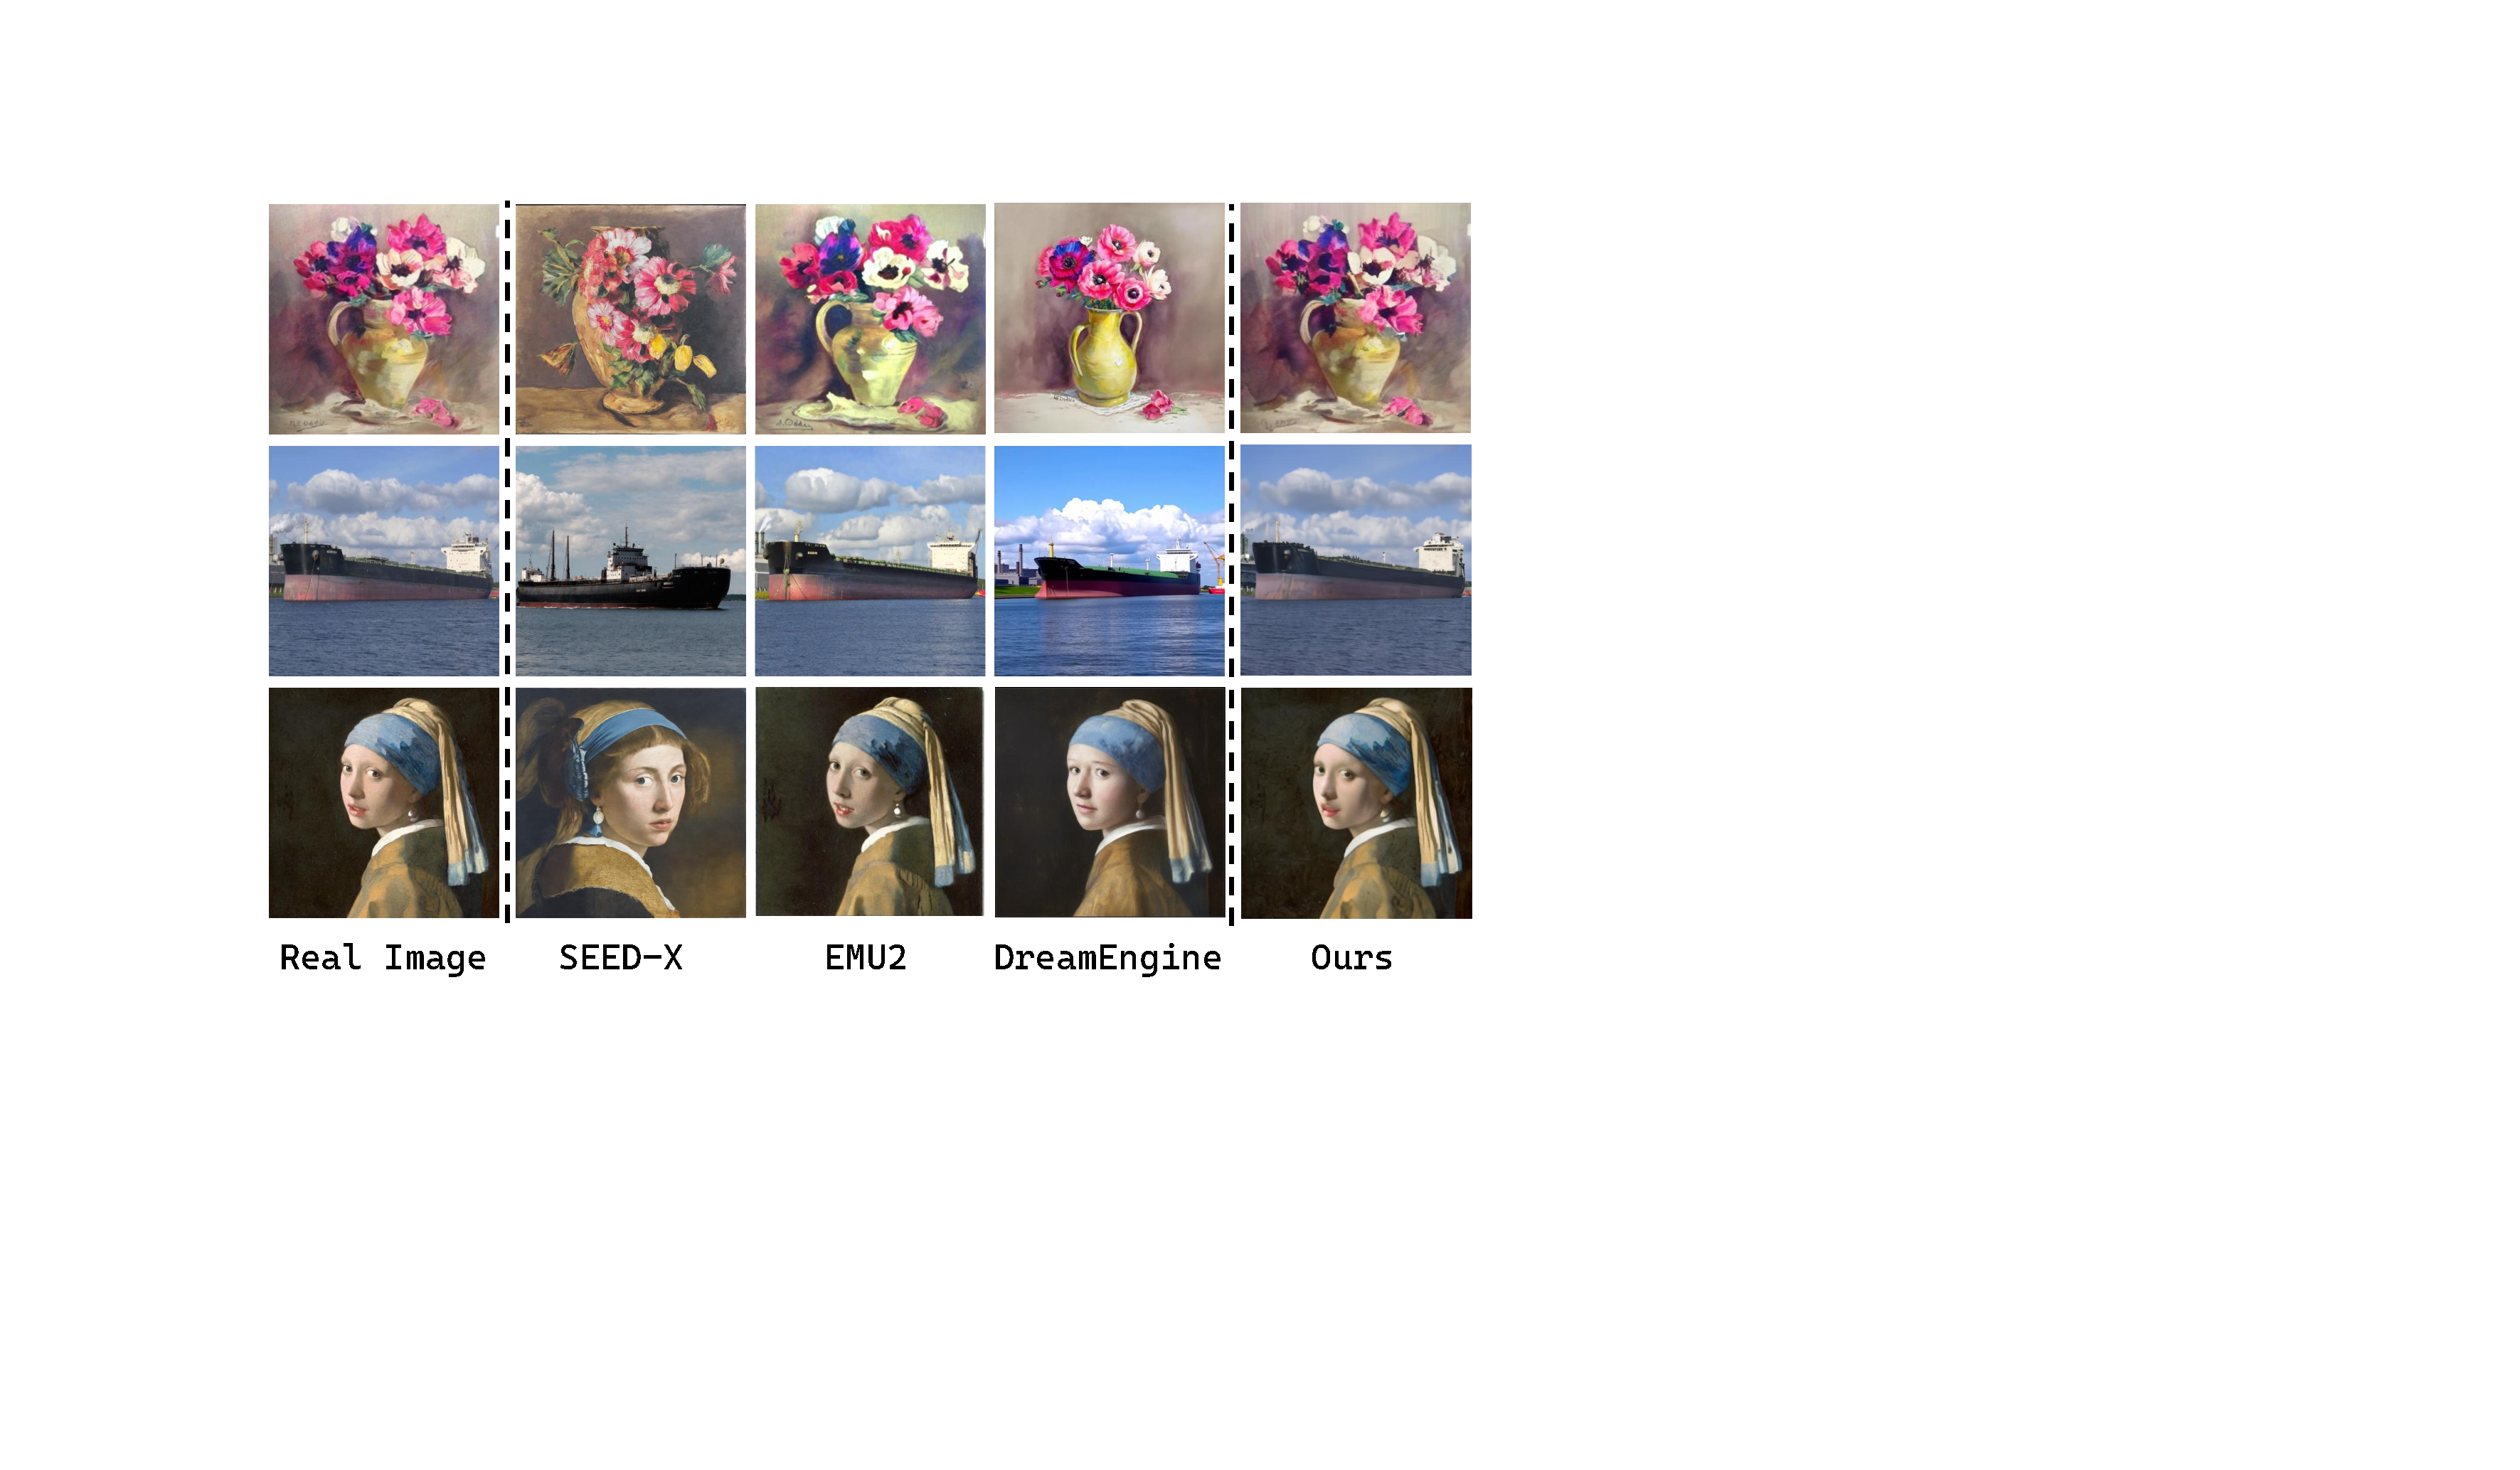
\includegraphics[width=\textwidth]{figures/reconstruction_exp.pdf}
%     \captionof{figure}{Image reconstruction results of various methods~\citep{dreamengine,2024SeedX,emu2}.}
%     \label{fig:reconstruction}
% \end{minipage}
% \end{figure*}



\begin{table}[t]
\vspace{-8ex}
\centering
\caption{Controllable experiments between \model and Kosmos-G in DreamBench++ benchmark.}
\label{tab:comparison}
\resizebox{\textwidth}{!}{%
\begin{tabular}{@{}lcccccccccc@{}}
\toprule
\textbf{Method} & \multicolumn{5}{c}{\textbf{Concept Preservation (CP)}} & \multicolumn{4}{c}{\textbf{Prompt Following (PF)}} & \textbf{CP$\cdotp$PF} \\ 
\cmidrule(lr){2-6} \cmidrule(lr){7-10}
 & \textbf{Animal} & \textbf{Human} & \textbf{Object} & \textbf{Style} & \textbf{Overall} & \textbf{Photorealistic} & \textbf{Style Transfer} & \textbf{Imaginative} & \textbf{Overall} & \\ 
\midrule
Kosmos-G  & 0.17 & 0.08 & 0.14 & 0.18 & 0.15 & 0.72 & 0.71 & 0.68 & 0.71 & 0.11 \\
\model     & 0.65 & 0.36 & 0.57 & 0.47 & \textbf{0.55} & 0.86 & 0.85 & 0.80 &\textbf{0.84} & \textbf{0.47} \\ 
\bottomrule
\end{tabular}%
}
\vspace{-2ex}
\end{table}


\begin{table}[t]
\centering
\vspace{-2ex}
\small
\caption{Ablation studies on architecture design and multi-image training}
\label{tab:ablation_combined}
\resizebox{\linewidth}{!}{%
\begin{tabular}{lcccccc}
\toprule
\multirow{2}{*}{\textbf{Method}} &
\multicolumn{3}{c}{\textbf{DreamBench++}} &
\multicolumn{3}{c}{\textbf{DreamBench}} \\
\cmidrule(lr){2-4} \cmidrule(lr){5-7}
 & \textbf{CP} & \textbf{PF} & \textbf{CP$\cdotp$PF} 
 & \textbf{DINOv1} & \textbf{CLIP-I} & \textbf{CLIP-T} \\
\midrule

\rowcolor{gray!10}
\textbf{\model}   
& $0.555 \pm 0.006$ & $0.839 \pm 0.002$ & $0.466$ 
& $70.853 \pm 0.327$  & $80.911 \pm 0.053$  & $29.071 \pm 0.080$ \\

\textit{w. Query-Variants}        
& $0.421 \pm 0.002$ & $0.882 \pm 0.000$ & $0.371$ 
& $54.518 \pm 0.317$  & $76.306 \pm 0.114$  & $30.792 \pm 0.040$ \\


\textit{w. Multi-image}         
& $0.586 \pm 0.006$ & $0.829 \pm 0.005$ & $\mathbf{0.486}$ 
& $72.487 \pm 0.147$ & $81.857 \pm 0.152$ & $28.545 \pm 0.043$ \\
\bottomrule
\end{tabular}%
}
\vspace{-2ex}
\end{table}


\textbf{Effect of Multi-Image Training.}
To assess the benefits of richer visual context, we further trained the model using a mix of Stage 2 data and additional multi-subject task(reconstructing images based on segmented objects and image caption) generated via our data construction pipeline. As shown in \Cref{tab:ablation_combined}, \textit{w. MultiImage Training} achieves a higher CP$\cdotp$PF score (0.49), improving CP to 0.60 while maintaining a strong PF score.
This emphasizes the advantage of enhanced visual context in training, prompting the model to efficiently handle and integrate information from multiple visual inputs, thereby improving its ability to preserve visual details in complex multimodal scenarios.

% To further investigate the effect of multi-image conditioning in multimodal generation, we continue training the model using a mixture of Stage 2 data and additional multi-subject samples generated via our data construction pipeline. In this setting, the model is tasked with reconstructing the original image based on segmented object crops and the corresponding image caption. Training is conducted for one additional epoch with a learning rate of 5e-5. Due to context length constraints, we limit each example to a maximum of three sub-images, resulting in a total sequence length of 888 tokens.



% \begin{table}[t]
% \centering
% \small
% \caption{Comparison of proposed variants across the DreamBench++ benchmark.}
% \label{tab:comparison}
% \resizebox{\textwidth}{!}{%
% \begin{tabular}{@{}lcccccccccc@{}}
% \toprule
% \textbf{Method} 
% & \multicolumn{5}{c}{\textbf{Concept Preservation (CP)}} 
% & \multicolumn{4}{c}{\textbf{Prompt Following (PF)}} 
% & \textbf{CP$\cdotp$PF} \\
% \cmidrule(lr){2-6} \cmidrule(lr){7-10}
% & \textbf{Animal} & \textbf{Human} & \textbf{Object} & \textbf{Style} & \textbf{Overall} 
% & \textbf{Photorealistic} & \textbf{Style Transfer} & \textbf{Imaginative} & \textbf{Overall} 
% & \\
% \midrule
% \rowcolor{gray!10} \textbf{Ours-MLP-based}       & 0.65 & 0.36 & 0.57 & 0.47 & 0.55 & 0.86 & 0.85 & 0.80 & 0.84 & \textbf{0.47} \\
% \rowcolor{gray!10} \textbf{Ours-Query-based}     & 0.54 & 0.32 & 0.38 & 0.38 & 0.42 & 0.91 & 0.91 & 0.78 & 0.88 & 0.37 \\
% \rowcolor{gray!10} \textbf{Ours-MultiImage}      & 0.71 & 0.40 & 0.60 & 0.52 & 0.60 & 0.86 & 0.85 & 0.80 & 0.83 & 0.49 \\
% \bottomrule
% \end{tabular}%
% }
% \end{table}


\begin{wrapfigure}{r}{0.52\textwidth}  % r 表示靠右,宽度根据内容调整
    \centering
    \vspace{-3ex}
    \begin{minipage}{0.9\linewidth}
        \centering
        \footnotesize
        \captionof{table}{Image reconstruction performance.}
        \vspace{-1ex}
        \label{tab:reconstruct_l2}
        \resizebox{\linewidth}{!}{
        \begin{tabular}{@{}lcc@{}}
        \toprule
        \textbf{Method} & \textbf{COCO ($\downarrow$)} & \textbf{JourneyDB ($\downarrow$)} \\
        \midrule
        SeedTokenizer   & 0.5102 & 0.5291 \\
        SEED-X          & 0.4317 & 0.4352 \\
        EMU2-Gen        & 0.3828 & 0.2869 \\
        DreamEngine     & \underline{0.2065} & \underline{0.2052} \\
        \midrule
        \textbf{\model}   & \textbf{0.1008} & \textbf{0.0867} \\
        \bottomrule
        \end{tabular}
        }
    \end{minipage}
    \vspace{1ex}
    
    \begin{minipage}{\linewidth}
        \centering
        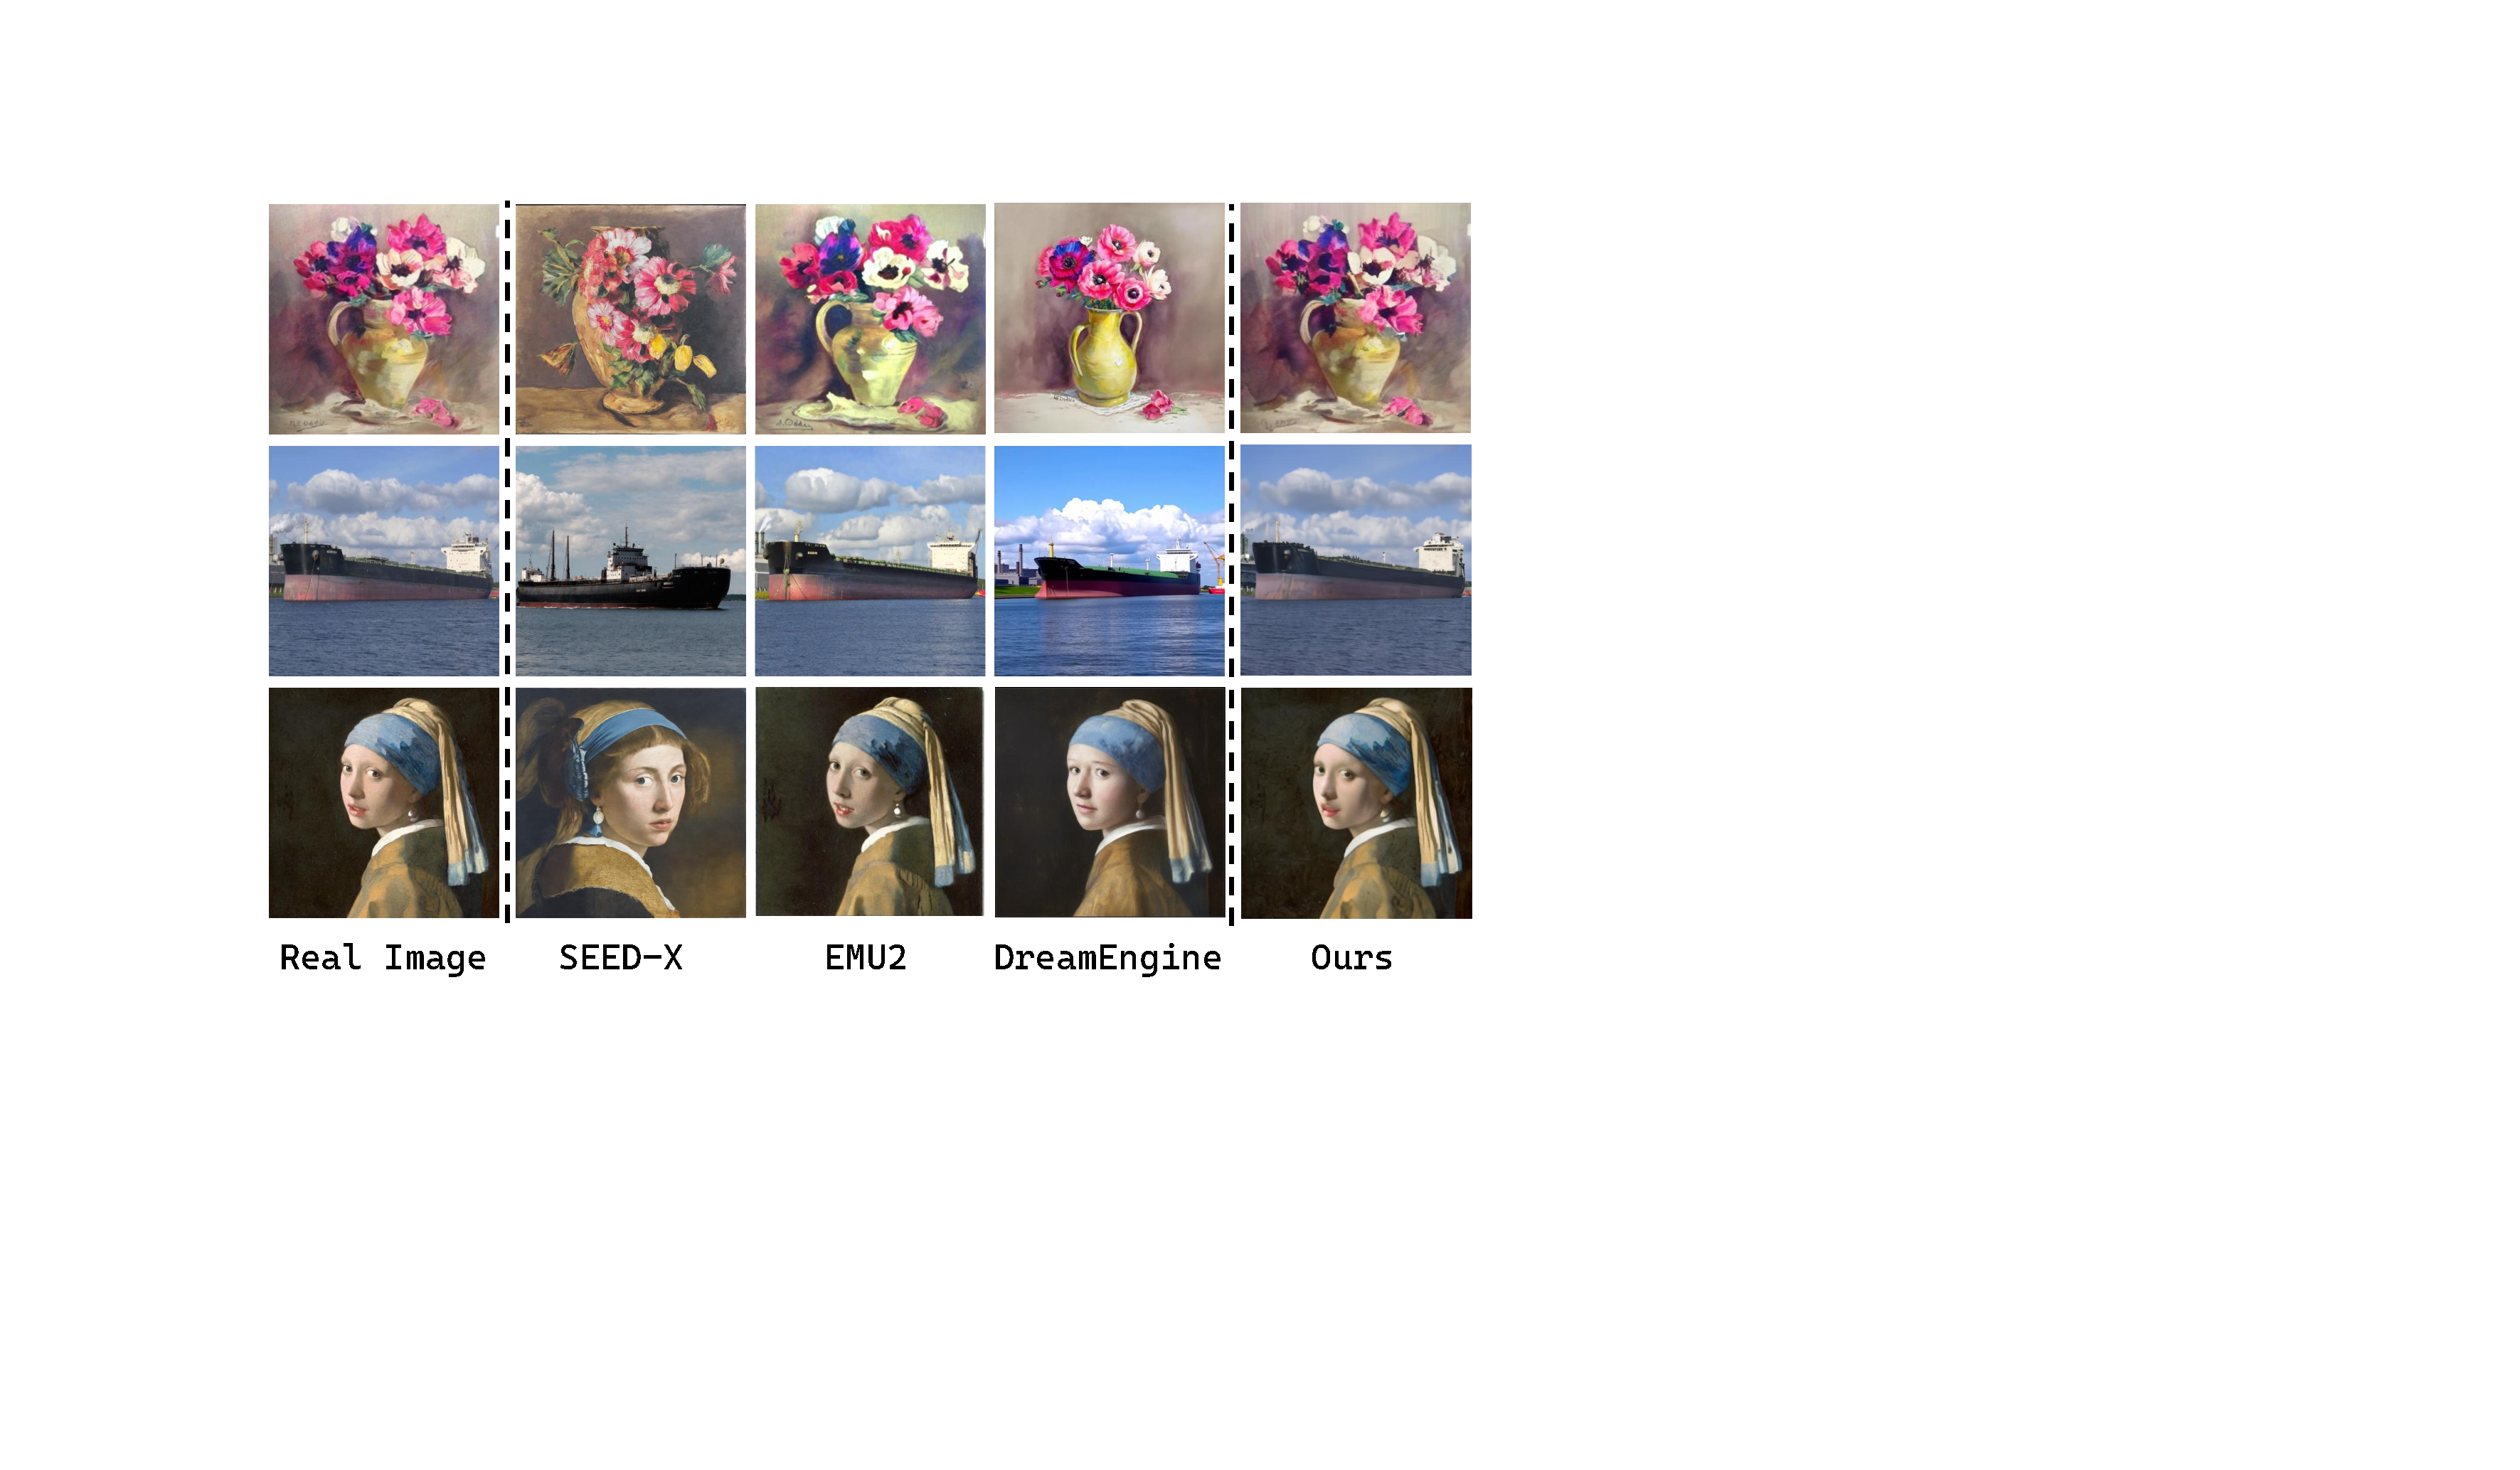
\includegraphics[width=\linewidth]{figures/reconstruction_exp.pdf}
        \vspace{-3ex}
        \captionof{figure}{Qualitative study on Image Reconstruction.}
        \label{fig:reconstruction}
    \end{minipage}
    \vspace{-5ex}

\end{wrapfigure}

\textbf{Image Reconstruction Fidelity.}
To quantify visual detail preservation in our framework, we evaluate \model on the Image Reconstruction Benchmark~\citep{dreamengine}, which measures similarity between input and reconstructed images. After fine‑tuning on reconstruction task for 1{,}000 steps, we compare the generated outputs with their originals using pixel‑space $\ell_2$ distance, following pervious work~\citep{dreamengine}. As shown in \Cref{tab:reconstruct_l2}, \model outperforms strong baselines with comparable architectures—SeedTokenizer~\citep{seed-tokenizer}, EMU2~\citep{emu2}, SeedX~\citep{2024SeedX}, and DreamEngine~\citep{dreamengine}—all of which couple LMMs with diffusion backbones.
\model achieves the best reconstruction quality, exceeding the second-best by 50\%, even with a $224{\times}224$ receptive field, while others varied from 384x384 to 512x512.
% In particular, it improves upon the second‑best approach by 51.2\% (COCO) and 57.7\%(JourneyDB) in $\ell_2$ distance, demonstrating superior pixel-level fidelity even with a $224{\times}224$ receptive field, while others range from 384x384 to 512x512. 
These gains confirm our model’s effectiveness at conditioning on—and faithfully reproducing—visual inputs.




% We introduce an  to evaluate the preservation of visual features in our Image-to-Image alignment task. This capability is essential for generating images conditioned on input images. 
% Afte finetuning on image reconstrction task for 1000 steps, we assess the similarity between the original and reconstructed images generatd by our model using the CLIP~\citep{radford2021clip} score and L2-Distance from the images in JourneyDB and COCO dataset. As shown in \Cref{tab:reconstruct}, we compare the performance of our model against several baselines with similar architectures, including SeedTokenizer~\citep{seed-tokenizer}, EMU-2~\citep{emu2}, SeedX~\citep{2024SeedX}, and DreamEngine~\citep{dreamengine}, which also integrate LMMs and diffusion models for generation. The results demonstrate that our model achieves the best average image reconstruction performance across both subsets of the benchmark. It notably surpasses the second-best by xx on the COCO and xx on the JourneyDB subsets in terms of L2 distance, highlighting its pixel-level consistency, albeit at an image receptive field of 224×224, while others varied from 384x384 to 512x512.


\textbf{Versatility Across Different Multimodal Tasks.}
To explore broader applicabilities of our framework, we evaluate its adaptability across diverse generation tasks, including image segmentation,  multi-image generation and multimodal in-context image generation. This was achieved with brief fine-tuning on relevant datasets, as detailed in~\Cref{app:applications}. Qualitative results in \Cref{fig:examples} show that the \model produces coherent, high-quality outputs that adhere to the provided constraints without requiring any architectural modifications. While achieving  performance in each specific domain would necessitate more specialized training and potentially more powerful multimodal encoder and generator components, these initial results underscore our framework's versatility and its potential as an effective foundation for a variety of multimodal conditional image generation applications.
 

% \paragraph{\mbox{Text-to-Image Generation}}

% We evaluate the text-to-image generation capability of our model on the COCO-40K benchmark. The results are presented in Table \ref{tab:fid_comparison}. Built upon the LlamaGen model~\citep{llamagen}, limited by the performance of the generator, our model shows much lower text-image generation ability than other baselines. However, thanks to the effective understanding of multimodal input, our model can balance these two different modalities, and with high-quality instruction following ability, ultimately further exceed other baselines in multimodal conditional image generation.
%  image segmentation set where? show cases additional task, editing; 



% \begin{table}[t]
% \centering
% \caption{Image reconstruction performance (L2 distance) on COCO and JourneyDB datasets.}
% \label{tab:reconstruct_l2}
% \resizebox{0.5\textwidth}{!}{
% \begin{tabular}{@{}lcc@{}}
% \toprule
% \textbf{Method} & \textbf{COCO ($\downarrow$)} & \textbf{JourneyDB ($\downarrow$)} \\
% \midrule
% SeedTokenizer              & 0.5102          & 0.5291          \\
% EMU2-Gen                  & 0.3828 & 0.2869 \\
% SEED-X                    & 0.4317          & 0.4352          \\
% DreamEngine               & \underline{0.2065}          & \underline{0.2052}          \\
% \midrule
% \textbf{Ours}             & \textbf{0.1008} & \textbf{0.0867} \\
% \bottomrule
% \end{tabular}
% }
% \end{table}



% \begin{figure*}[htbp]
% \centering
% 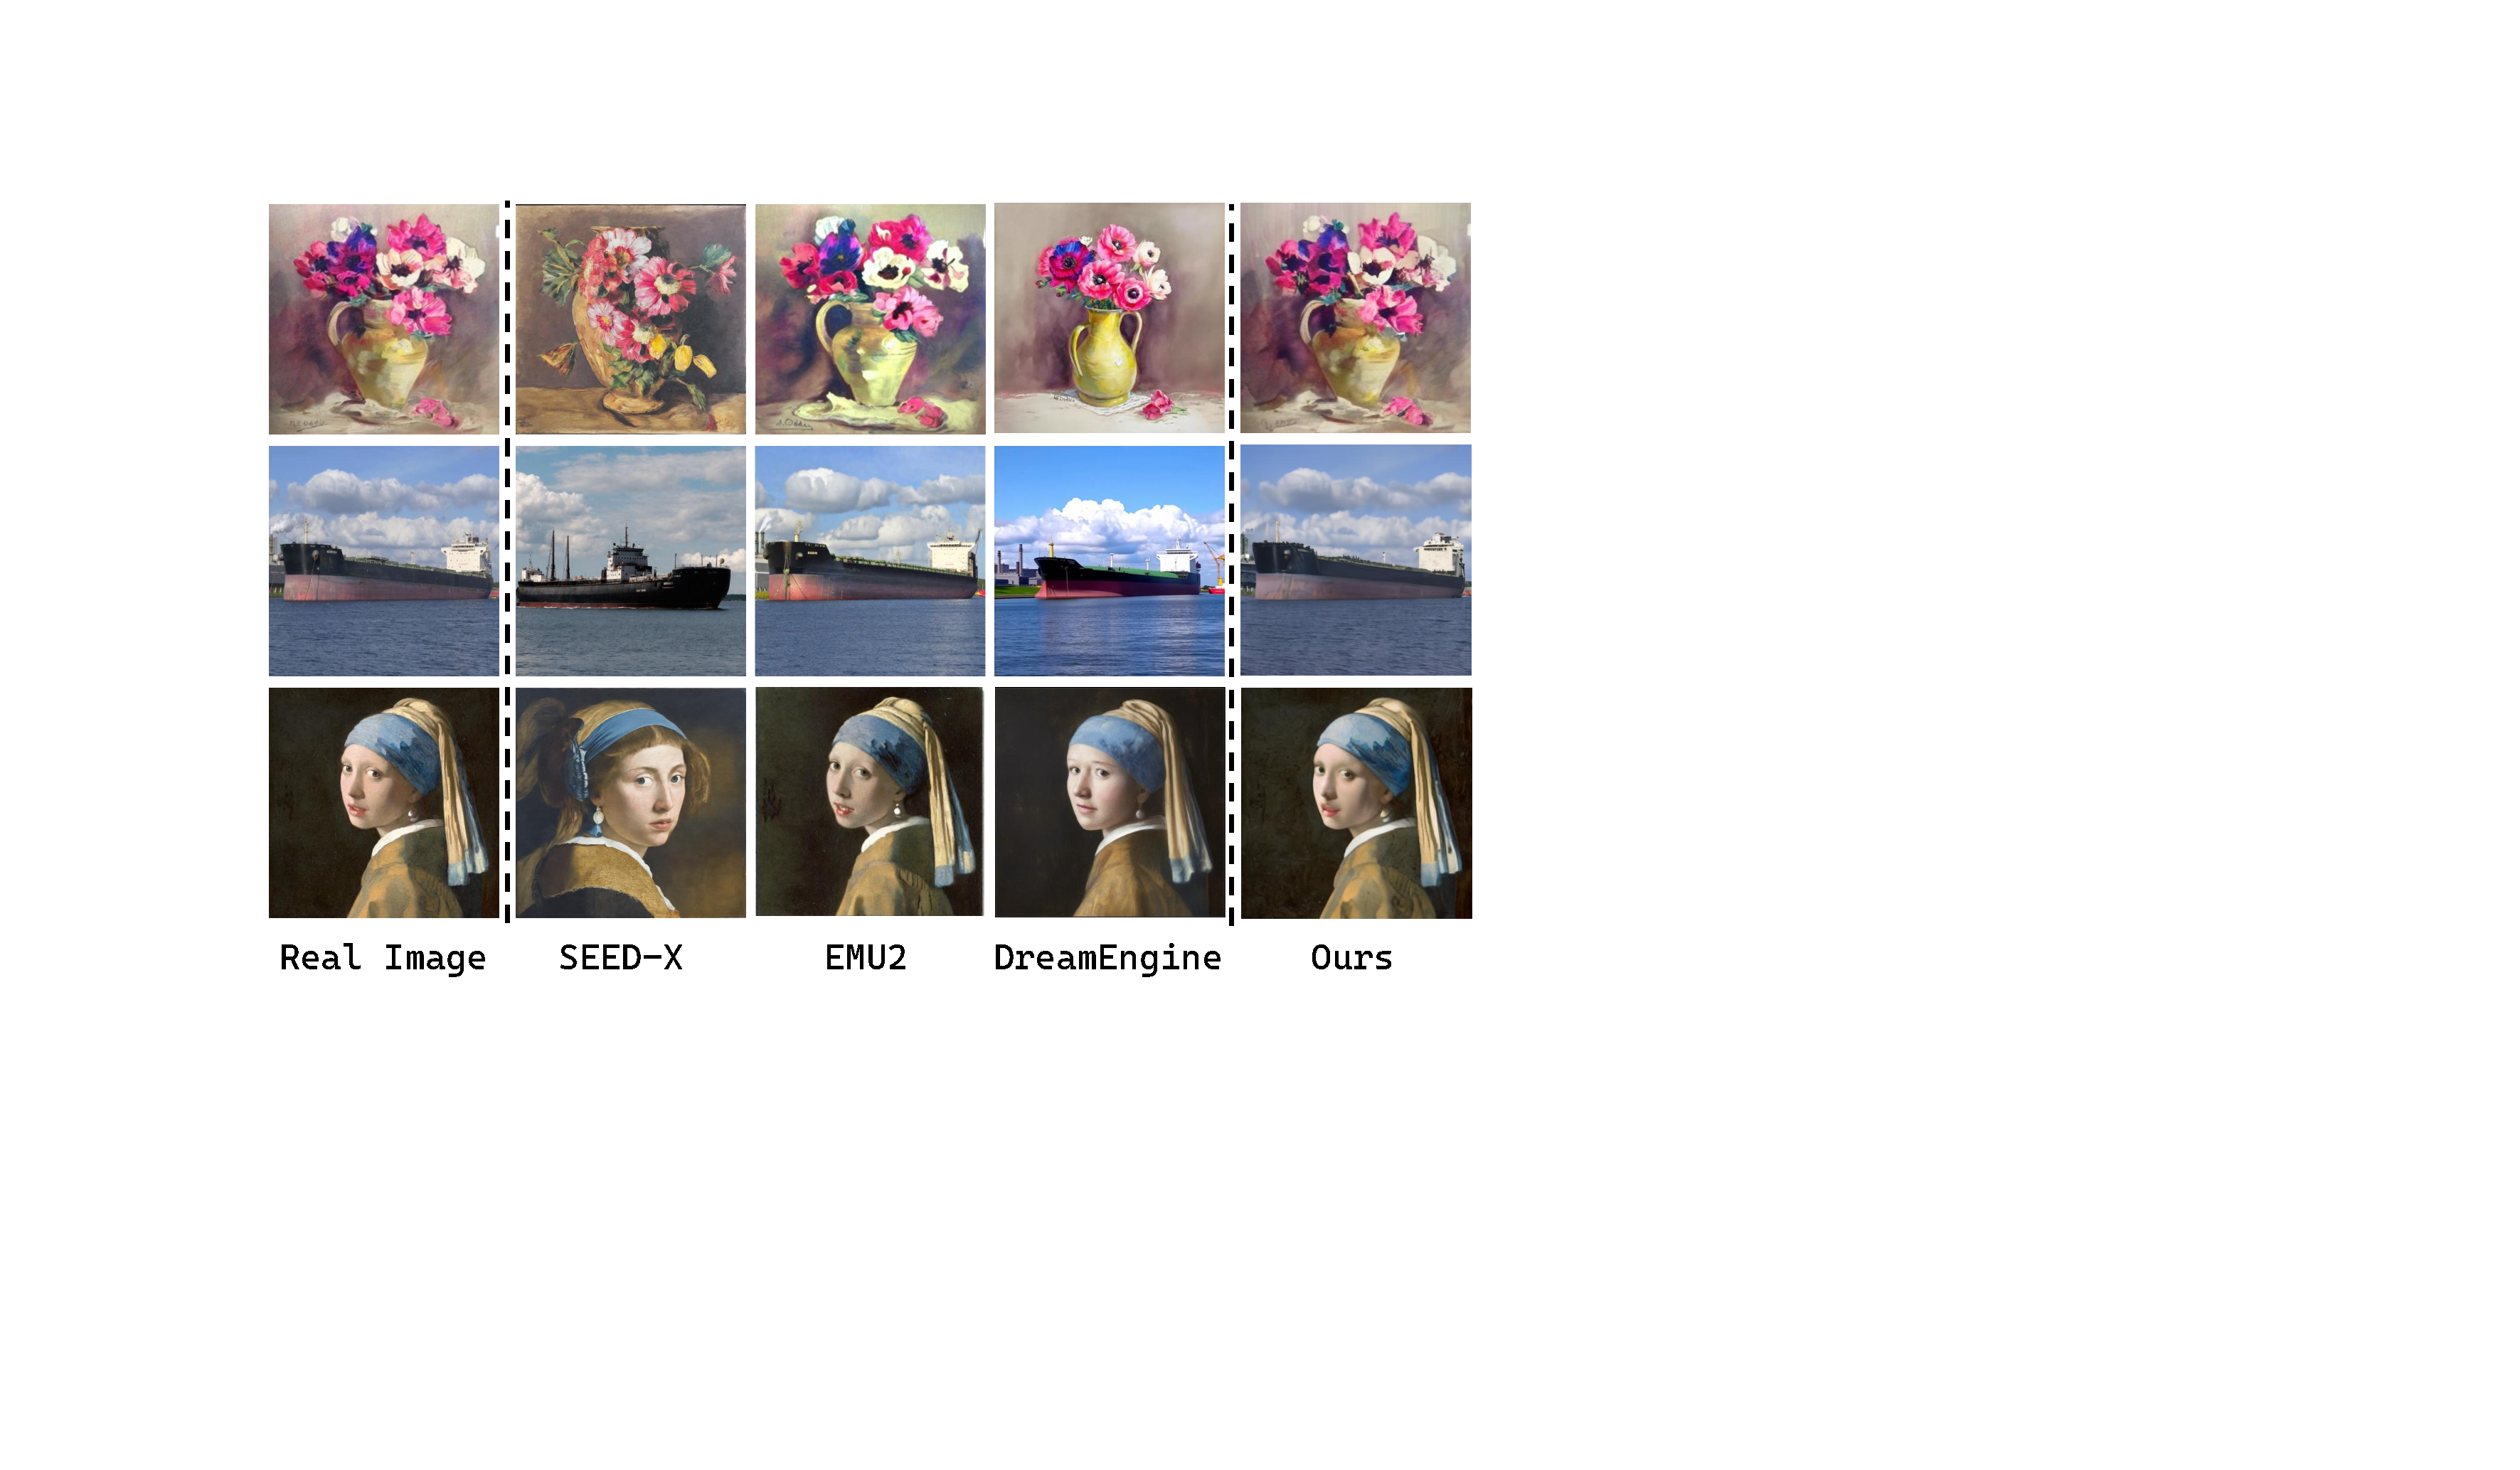
\includegraphics[width=1.0\textwidth]{figures/reconstruction_exp.pdf}
% \caption{Comparison of image reconstruction results among different methods~\citep{dreamengine,2024SeedX,emu2}.}
% \label{fig:reconstruction}
% \end{figure*}


% \begin{table}[t]
% \centering
% \caption{Image reconstruction performance comparison on COCO and JourneyDB datasets.}
% \label{tab:reconstruct}
% \resizebox{0.47\textwidth}{!}{
% \begin{tabular}{@{}lcccc@{}}
% \toprule
% \multirow{2}{*}{\textbf{Method}} & \multicolumn{2}{c}{\textbf{COCO}} & \multicolumn{2}{c}{\textbf{JourneyDB}} \\
% \cmidrule(lr){2-3} \cmidrule(lr){4-5}
%  & CLIP~($\uparrow$) & L2~($\downarrow$) & CLIP~($\uparrow$) & L2~($\downarrow$) \\
% \midrule
% SeedTokenizer              & 0.7760          & 0.5102          & 0.7921          & 0.5291 \\
% EMU2-Gen                  & 0.8537          & \underline{0.3828} & \textbf{0.9299} & \underline{0.2869} \\
% SEED-X                    & \underline{0.8595} & 0.4317          & 0.9017          & 0.4352 \\
% DreamEngine               & \textbf{0.8714} & 0.2065          & 0.9221          & 0.2052 \\

% \midrule
% Ours & 0.8335          & \textbf{0.1008}    & \underline{0.9062}   & \textbf{0.0867} \\
% \bottomrule
% \end{tabular}
% }
% \end{table}







% \paragraph{Image Segmentation}


% BLIP

% Llava

% Diffusion (Kosmos-G with our 1 stage training)


% \paragraph{Generation with Text-Image Interleaved Control}

% Upon completing Stage 2 training, our model gains the ability to integrate multimodal control within the image generation process. To assess our proposed paradigm of image generation capability under text-image interleaved control, we further train the model using a mixture of multi-image data. 

% In this paper, we demonstrate several applications of the model and evaluate its performance against Emu-2~\citep{emu2}, the most pertinent baseline which also facilitates text-image interleaved control.



% % \section{Related Work}
\label{sec:relatedwork}



% \begin{table}[htbp]
%   \centering
%   \setlength{\tabcolsep}{5pt}
%   \renewcommand{\arraystretch}{1.25}
%   \begin{tabular}{lccccccc}
%     \toprule
%     \textbf{Model} &
%     T$\Rightarrow$I &
%     I+T$\Rightarrow$T &
%     T+I$\Rightarrow$T+I &
%     Open-source &
%     Available &
%     \makecell[c]{Actual\\Support\\T+I$\Rightarrow$I} &
%     \makecell[c]{Within\\3 Month} \\
%     \midrule
%     EMU3              & \cmark & \cmark &        & \cmark & \cmark &        &        \\
%     LWM               & \cmark & \cmark &        & \cmark & \cmark & no train   &        \\
%     Unified-IO2       & \cmark & \cmark & ?      & \cmark & \cmark & \cmark &        \\
%     Lumina-mGPT       & \cmark & \cmark & \cmark & \cmark & \cmark & \cmark &        \\
%     Lumina-mGPT 2.0   & \cmark & \cmark & \cmark & \cmark &        &  no train   & \cmark \\
%     Liquid            & \cmark & \cmark &        & \cmark & \cmark & \cmark &        \\
%     vargpt            & \cmark & \cmark & ?      & \cmark & \cmark & ?      &        \\
%     vargpt-1.1        & \cmark & \cmark & \cmark & \cmark & \cmark & \cmark & \cmark \\
%     VILA-U            & \cmark &        & no train   & \cmark & \cmark & no train   &        \\
%     Janus             & \cmark & \cmark &        & \cmark & \cmark &        &        \\
%     MUSE-VL           & \cmark & \cmark &        &        &        &        &        \\
%     X-Prompt          & \cmark & \cmark & \cmark &        &        & \cmark &        \\
%     \bottomrule
%   \end{tabular}
%   \caption{Multimodal model capability and availability overview.}
%   \label{tab:model_overview}
% \end{table}



% \subsection{Image Generation with Complex Control}
% % blipdiffusion, kosmos-g, emu2, subject-diffusion, suti, control net
% Recent progress in controlled image generation using diffusion models has been significant. Researchers have explored various conditioning strategies—ranging from low-level cues like canny edges and depth maps~\citep{ye2023ip-adapter, controlnet} to higher-level guidance provided by reference images~\citep{SDEdit}—to steer the generative process. For instance, methods such as IP-Adapter~\citep{ye2023ip-adapter} and ControlNet~\citep{controlnet} incorporate additional control signals into standard text-to-image frameworks, thereby allowing more precise manipulation of generated content.
% In parallel, several works have leveraged visual elements from input images to further guide the generation process. DreamBooth~\citep{ruiz2023dreamboothfinetuningtexttoimage} and Textual Inversion~\citep{gal2022imageworthwordpersonalizing}, for example, adopt optimization-based approaches to adapt models to specific reference images. Although effective, these methods typically require extensive fine-tuning for each new input, limiting their practicality. To address these limitations, approaches like SuTI~\citep{suti} and Subject-diffusion~\citep{ma2024subjectdiffusionopendomainpersonalizedtexttoimage} have aimed to scale the fine-tuning process so that models can generalize across diverse reference images. However, these strategies still tend to be both time- and resource-intensive, highlighting the ongoing need for more efficient mechanisms for image generation with complex controls.

\subsection{Image Generation with Complex Multimodal Control}
Researchers have developed image generation via diffusion models conditioned on multimodal inputs like canny edges~\citep{controlnet} and reference images~\citep{ultraEdit,SDEdit}. ControlNet~\citep{controlnet} uses auxiliary parameters, while Mix-of-Show~\citep{Mix-of-Show} and FLUXSynID~\citep{FLUXSynID} use LoRA modules for multi-concept control and identity preservation.
DreamBooth~\citep{ruiz2023dreamboothfinetuningtexttoimage} enable subject-specific fine-tuning but limit generalization. SuTI~\citep{suti} address it with scalable data and training.
To enhance flexibility, recent work integrates LMMs with diffusion models by mapping LMM embedding into diffusion spaces~\citep{koh2023GILL,sun2023emu1,dreamllm,unimo}. Approaches like Kosmos-G~\citep{Kosmos-G}, Emu-2~\citep{emu2}, Seed-X~\citep{2024SeedX}, and DreamEngine~\citep{dreamengine} explore more complex multimodal prompt and fine-grained multimodal control. Yet, balancing guidance from diverse modalities remains a core challenge~\citep{han2024emmatexttoimagediffusionmodel,ye2023ip-adapter,RealCustom++}. 
EMMA~\citep{han2024emmatexttoimagediffusionmodel} employs a gated perceiver resampler for dynamic signal integration, while RealCustom++\citep{RealCustom++} disentangles subject identity and textual fidelity via cross-layer projectors. OmniControl~\citep{OminiControl} introduces a bias term into multimodal attention. 
Nonetheless, these method often require substantial computational resources, and achieving efficient, robust, and scalable multimodal integration remains an open problem.



\subsection{Autoregressive Multimodal Image Generation}
Autoregressive models have driven progress in T2I generation, from DALL·E~\cite{DALLE} and Parti~\citep{parti} to LlamaGen~\citep{llamagen} and GPT4O~\citep{gpt4o}.
Recent work extends it to multimodal settings: Models like Chameleon~\citep{chameleonteam2024chameleon}, LWM~\cite{LWM}, AnyGPT~\citep{Zhan2024AnyGPT}, and EMU3~\citep{Emu3} treat text and images as unified token sequences via early-fusion transformers, yet still emphasize text-to-image generation with limited support for multimodal conditioning.
Janus~\citep{Janus} decouples visual understanding and generation via distinct pathways, lacks support for multimodal image generation. MUSE-VL~\cite{musevl} and VILA-U~\citep{VILA-U}  align discrete visual tokens with text to improve perception, but remain oriented toward understanding tasks rather than image generation.
Unified-IO2~\citep{lu2023unifiedio2} is trained autoregressively from scratch for both understanding and generation across modalities, while Lumina-mGPT~\cite{2024lumina} enhances Chameleon with omnipotent supervised fine-tuning for broader multimodal tasks. Nonetheless, these models often over-rely on visual inputs while ignoring textual prompts.
Overall, while models like VILA-U~\cite{VILA-U}, EMU3~\cite{Emu3}, and Janus~\cite{Janus} have advanced text-to-image generation, robust multimodal conditional image generation remains an open and underexplored challenge.


% % \section{Conclusion}
\label{sec:conclusion}

In this work, we introduced a controllable and efficient autoregressive framework for complex multimodal image generation, offering a compelling alternative to diffusion-based methods.
By unifying multimodal inputs within an AR model and leveraging a two-stage training paradigm, our method achieves state-of-the-art performance on challenging benchmarks—despite a modest model size, suboptimal base component, and limited training resources.
These results underscore efficiency, scalability, and controllability of our method, establishing it as a efficient foundation for building versatile, fine-grained visual generation systems capable of handling complex multimodal prompts.

% By unifying multimodal inputs within AR framework and employing a two-stage training paradigm, our framework achieves state-of-the-art performance on complex benchmarks, demonstrating its efficiency, scalability, and controllability, even with a modest model size and significantly reduced training resources. This work establishes autoregressive models as a practical and scalable solution for multimodal image generation, laying a solid foundation for building versatile and controllable systems capable of nuanced visual generation from complex prompts.




% In this work, we have introduced an efficient and controllable autoregressive framework for complex multimodal image generation, effectively addressing the limitations inherent to diffusion-based methods. Our approach leverages a unified autoregressive transformer architecture that integrates visual and textual inputs into a shared latent representation, enabling precise token-level control and alignment without auxiliary adapters or cross-attention blocks. Crucially, our novel two-stage training paradigm—comprising a multimodal alignment stage and a multimodal instruction tuning stage—ensures robust multimodal alignment and balanced modality conditioning, achieving substantial improvements in generation fidelity and instruction adherence.
% Extensive experiments demonstrate our framework's superior performance, surpassing state-of-the-art diffusion models despite employing significantly smaller architectures and reduced training resources. Our results highlight the effectiveness and scalability of autoregressive models in multimodal image generation tasks, establishing them as viable alternatives to diffusion-based counterparts. 
% Moving forward, our methodology offers a promising foundation for developing efficient, versatile, and controllable multimodal generative systems, paving the way for broader applications requiring precise and nuanced visual generation from complex multimodal prompts.





% \clearpage
\appendix
\section{Technical Appendices and Supplementary Material}
\noindent This Supplementary Material is organized as follows.  

\begin{itemize}[left=0pt]
    \item In \Cref{sec:Exp_Details}, we provide the training details of \model, including initialization (\Cref{sec:init_Details}), training procedures (\Cref{sec:tra_Details}), and multi-image training strategy(\Cref{sub:multi_init_Details}).
    \item In \Cref{sup:t2i}, we show quantitative evaluations of our method on text-to-image generation benchmarks.
    \item In \Cref{sec:data_const}, we detail our data construction pipeline and the dataset details used across the two-stage training.
    \item In \Cref{sec:Experiment_Details}, we elaborate on the experimental setup, including datasets and metrics (\Cref{sec:Benchmark_Details}), as well as detailed descriptions of baseline methods(\Cref{sec:Baselines_Details}).
    \item In \Cref{sec:Qualitative_Study}, we present qualitative results that demonstrate the capabilities of \model in various settings, such as image reconstruction(\Cref{sec:Reconstruction}), segmentation(\Cref{sec:Segmentation}), multi-image generation(\Cref{sec:Multi-Image}), and in-context image generation(\Cref{sec:mmicl}).
    \item In \Cref{app:applications}, we demonstrate the versatility of \model across diverse multimodal generation tasks, including segmentation, subject-driven generation, and multimodal in-context learning.
    \item In \Cref{app:limitation}, we discuss the current limitations of our method, such as its dependence on autoregressive generators, generation fidelity, and safety considerations.
\end{itemize}


\section{Training Details}
\label{sec:Exp_Details}

\subsection{Initialization Details}
\label{sec:init_Details}

The multimodal encoder is initialized using the vision encoder from CLIP-Large-Patch14~\citep{Radford2021LearningTV}, with an image receptive field of $224 \times 224$, and the FlanT5-XL encoder~\citep{flant5}, with a context length of 512 tokens. This encoder converts each image into 256 tokens for use as context in the generator.

To implement the MLP-based projection, we train the MLP projector on the LLaVA-CC3M-Pretrain-595K dataset~\citep{liu2023llava}, following the alignment training setup used by LLaVA. Specifically, we freeze both the vision and text encoders (CLIP-Large-Patch14 and FlanT5-XL, respectively) and train only the MLP layers. The resulting pretrained MLP layers are then directly incorporated into the multimodal encoder of \model.


\begin{figure*}[htbp]
\centering
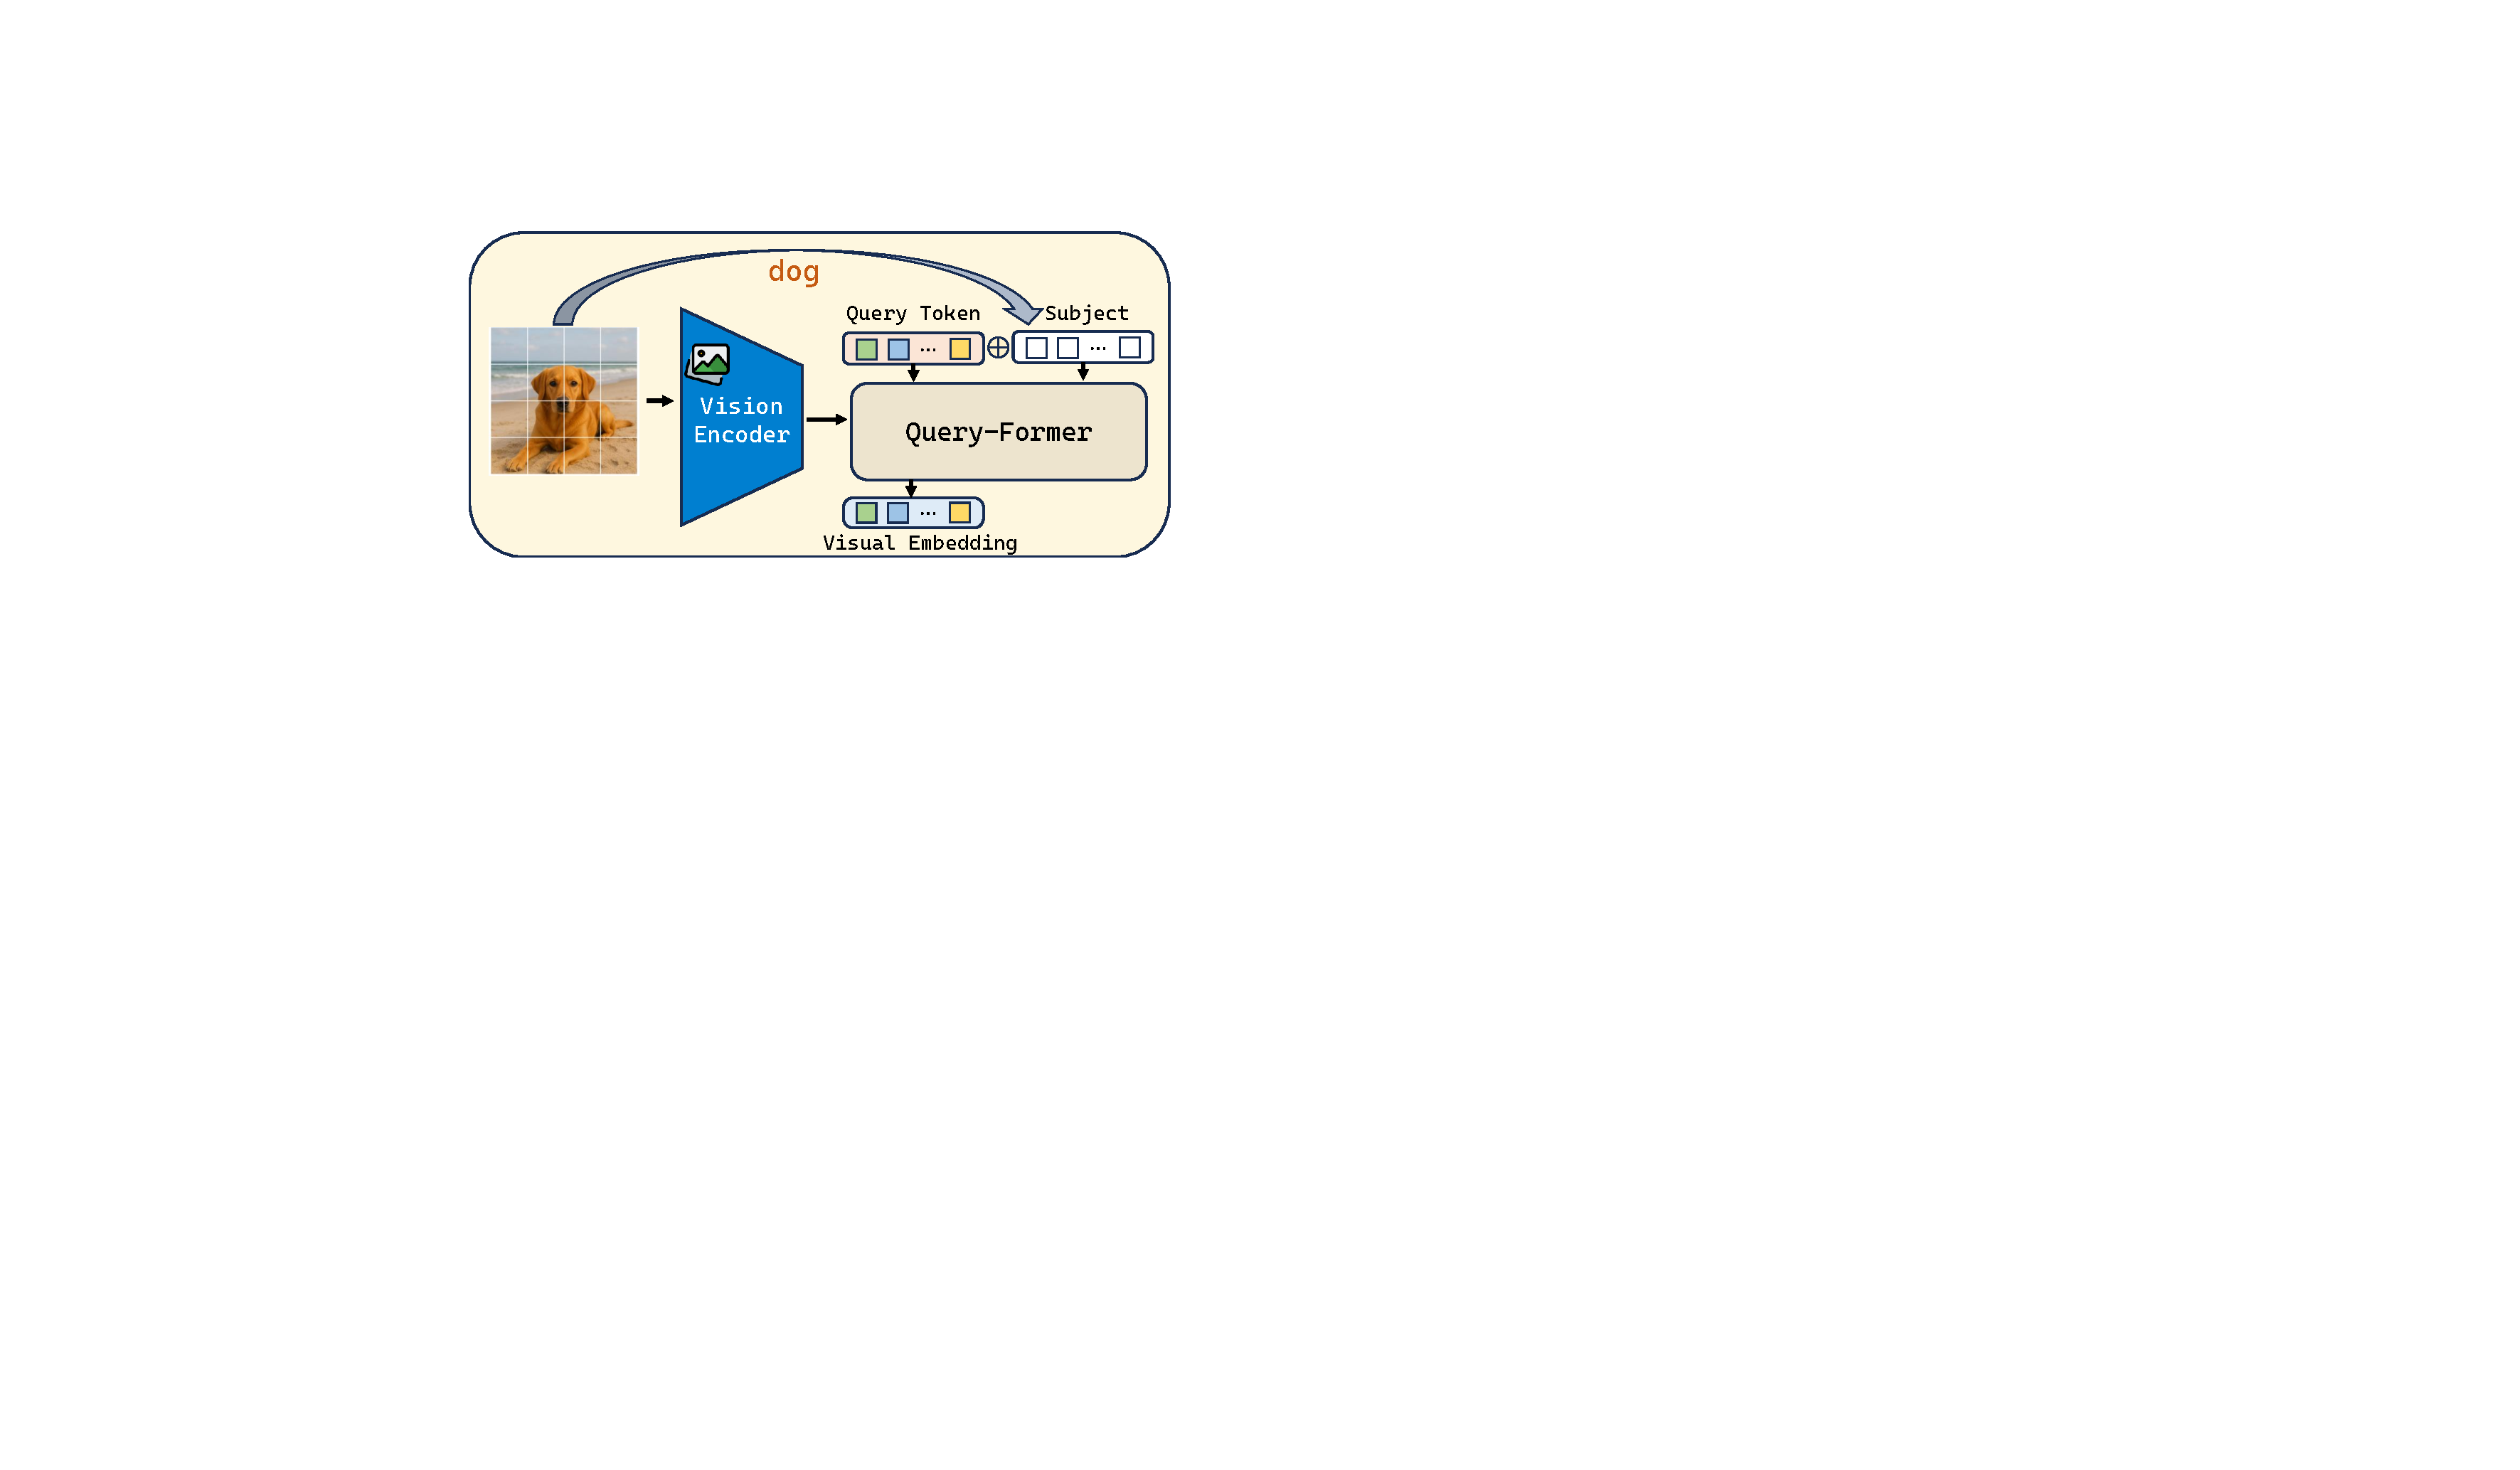
\includegraphics[width=0.8\textwidth]{figures/qformer.pdf}
\caption{Overview of text-guided visual distillation using the Query-based variant of \model.}
\label{fig:qformer}
\end{figure*}

The projector consists of a two-layer MLP with an intermediate dimension of 4,096, employing SiLU activation functions.
The autoregressive generator is initialized from LlamaGen-XL~\citep{llamagen} with 775 million parameters. 
However, the original LlamaGen implementation contains a fundamental error in its 2D Rotary Positional Embedding\citep{lu2023unifiedio2,EVA-02} (ROPE) mechanism\footnote{\url{https://github.com/FoundationVision/LlamaGen/issues/54}}, which leads to a loss of information in the query and key vectors during attention computation. To address this, we correct the ROPE implementation in our code and continue training the revised model on both the Midjourney dataset~\citep{midjourney-niji-1m-llavanext} and the LAION-COCO dataset used in LlamaGen pretraining, effectively replicating the original pretraining conditions. This continued training enables the model to adapt to the corrected ROPE mechanism. The resulting model is then used to initialize our autoregressive generator.

\subsection{Training Procedure}
\label{sec:tra_Details}

The model training comprises two distinct stages:

\textbf{Stage 1}: We freeze the multimodal encoder and train only the projector and generator modules for one epoch, using a global batch size of 128. Optimization employs the Adam optimizer with an initial learning rate of $5 \times 10^{-4}$, a linear warm-up over the initial 5% of steps, and a subsequent cosine decay schedule.

\textbf{Stage 2}: We fine-tune the entire model, excluding the vision encoder, for two epochs. The learning rate is reduced to $1 \times 10^{-4}$, with all other optimization settings remaining consistent with Stage 1. This phase primarily enhances cross-modal interactions and improves conditional image generation capabilities from combined visual and textual inputs.

Training is conducted across 8 NVIDIA A100 GPUs, each equipped with 80 GB memory, taking approximately 1.5 days. Specifically, Stage 1 training involves 2.48 million data points over a single epoch, completed in roughly 14 hours. Stage 2 training utilizes 1.3 million data points over two epochs, taking approximately 20 hours in total.

Ablation studies follow the same training schedule, with one epoch of training on Stage 1 data, followed by two epochs on Stage 2 data.

\subsection{Multi-Image Training}
\label{sub:multi_init_Details}
In \textbf{multi-image training} scenario, the context length of \model is expanded to 1,280 tokens to accommodate up to 4 images per context. For the Query-based variant of \model, token compression techniques enable processing up to 14 images per context with 512 context length.

We utilize 1.5 million multi-image samples, each comprising segmented sub-images accompanied by textual descriptions. The model is trained to reconstruct original images based on these segmented inputs and their corresponding captions. Training incorporates a mixture of Stage 2 data and multi-image samples for an additional epoch.

Qualitative assessments, presented in \Cref{fig:multi}, demonstrate that multi-image training significantly enhances the model's capability to preserve detailed visual information in complex multimodal contexts.

\begin{figure*}[t]
\centering
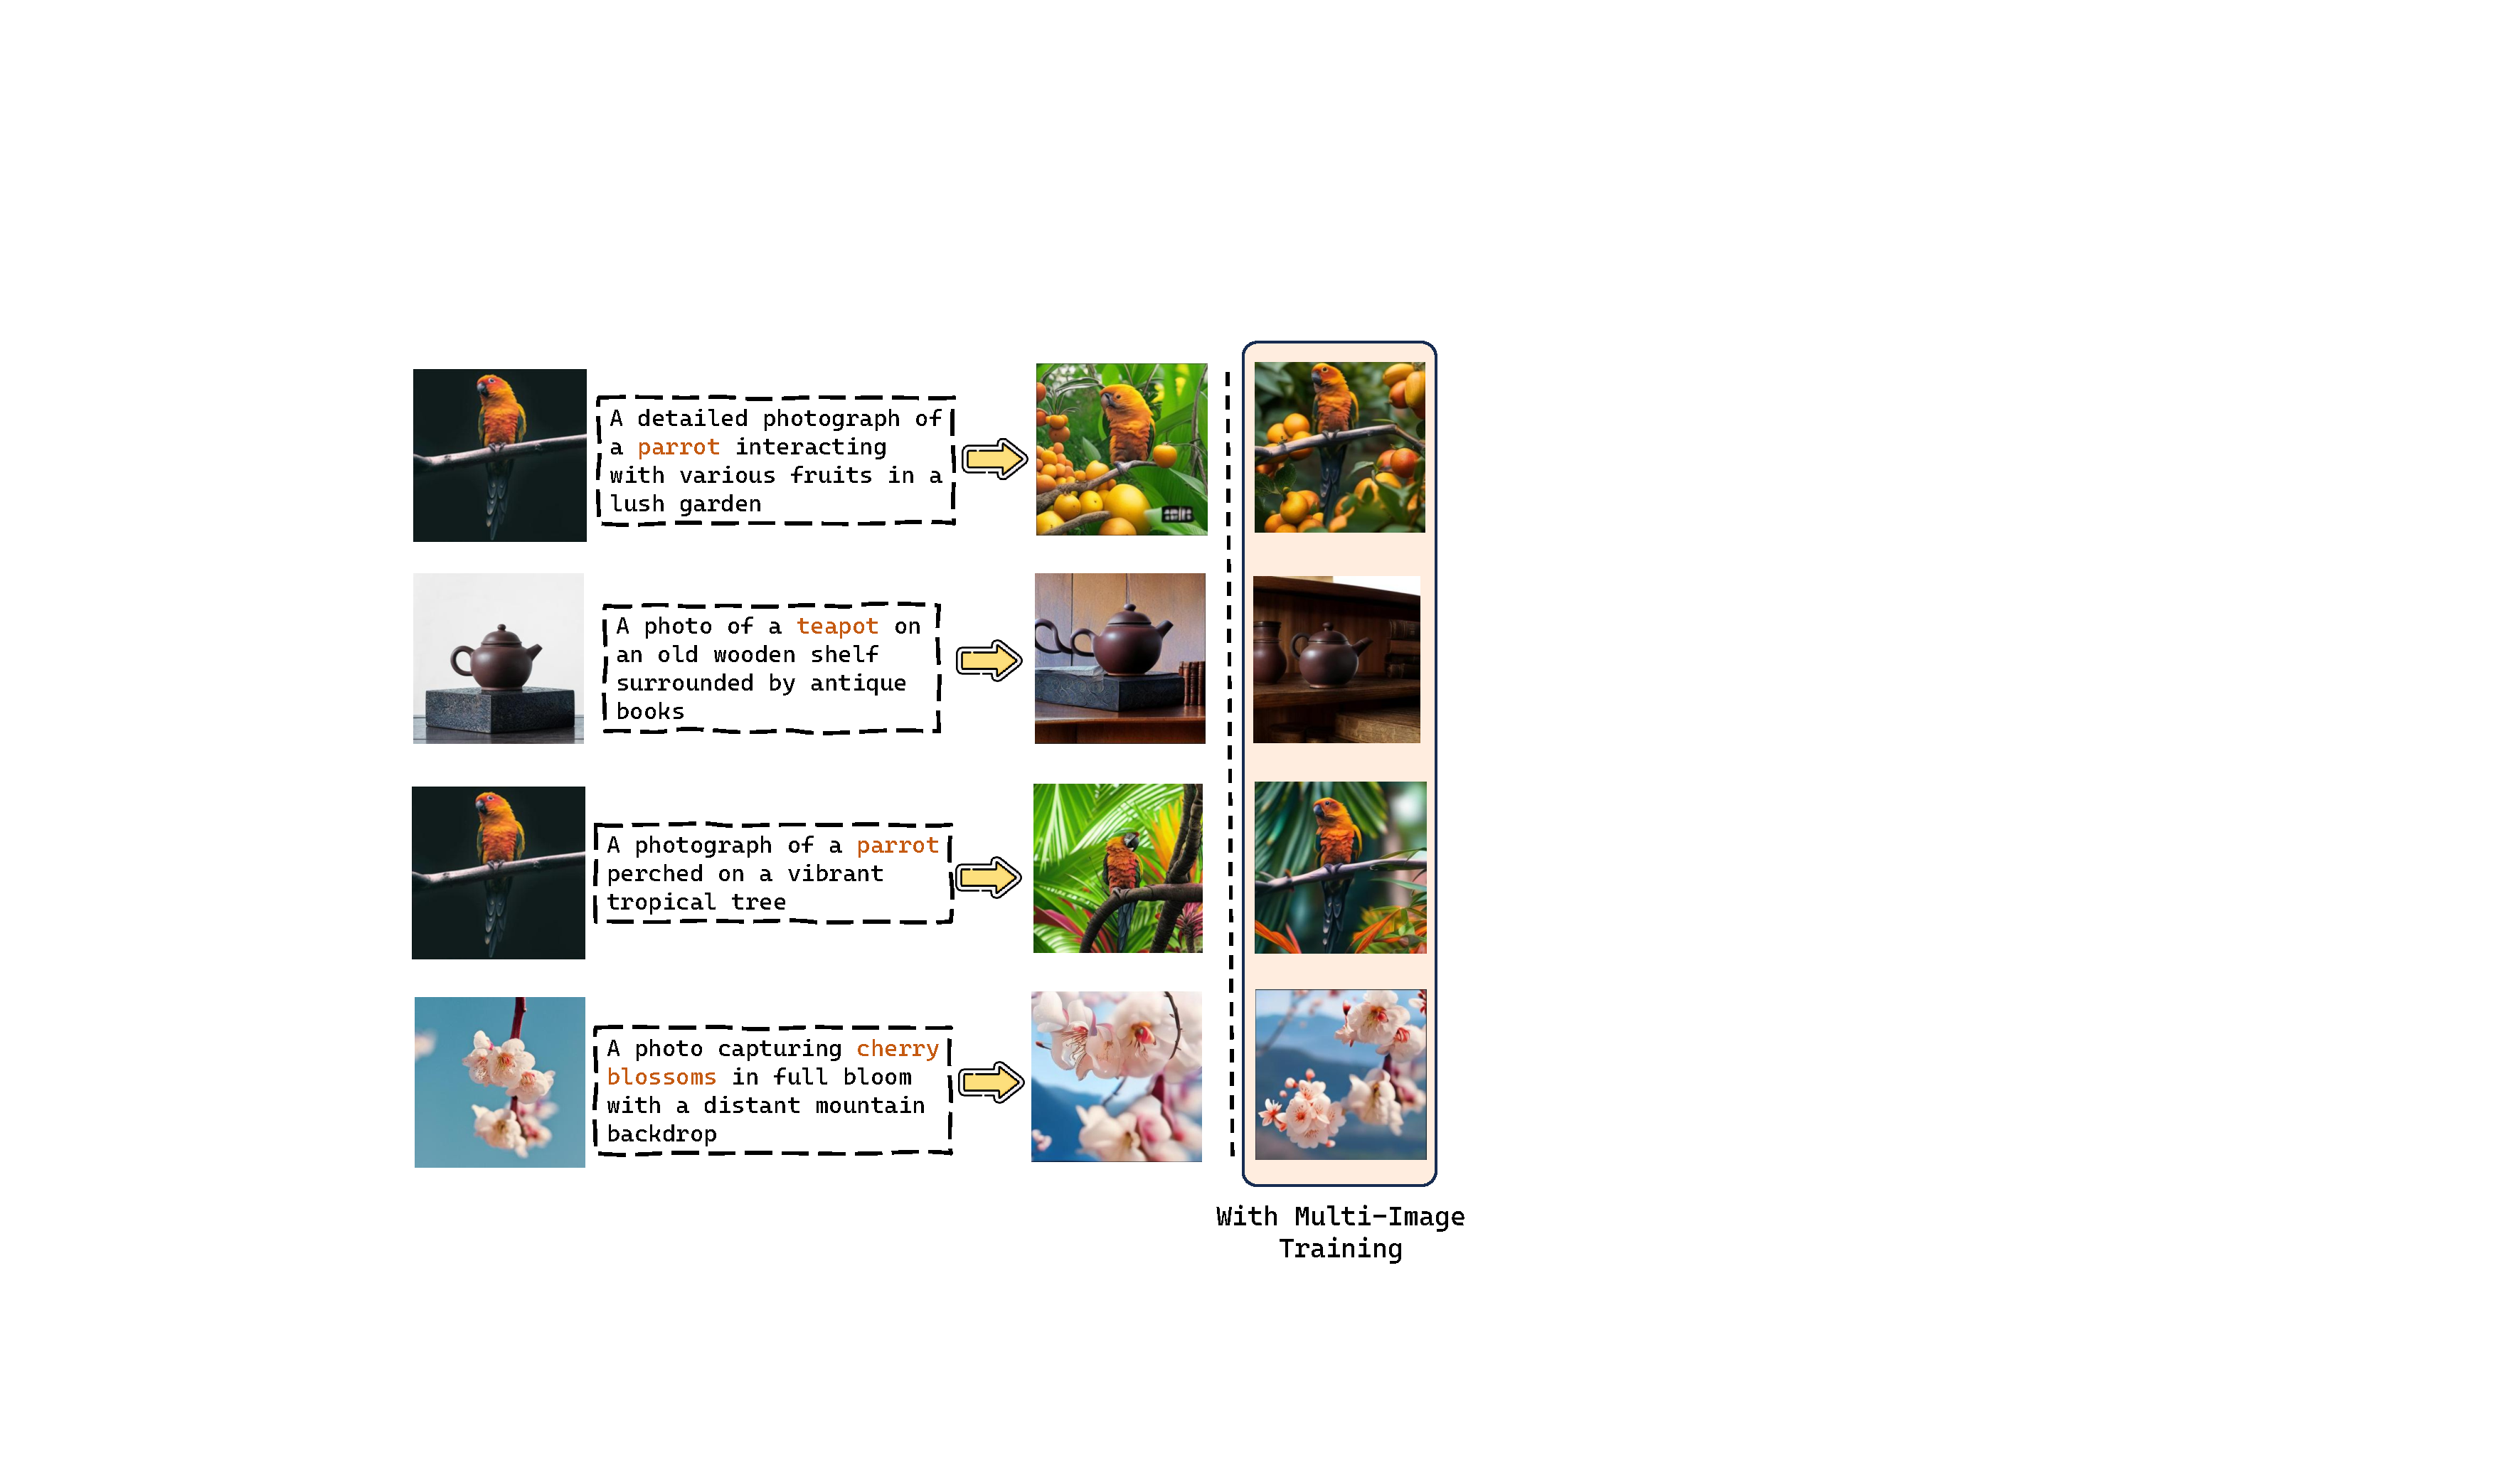
\includegraphics[width=1.0\textwidth]{figures/multi_exp.pdf}
\caption{Qualitative assessment demonstrating improved preservation of visual details by \model following multi-image training.}
\label{fig:multi}
\end{figure*}

\section{Text-to-Image Generation Evaluation}
\label{sup:t2i}
\begin{table*}[t]
    \centering
    \caption{GenEval benchmark results for text-to-image generation, classifying methods as either autoregressive or diffusion-based models. Due to our method's model size and suboptimal generators, we experience poor performance in text-to-image generation.}
    \resizebox{\textwidth}{!}{
    \begin{tabular}{@{}cl
        >{\centering\arraybackslash}m{1.4cm}
        >{\centering\arraybackslash}m{1.4cm}
        >{\centering\arraybackslash}m{1.4cm}
        >{\centering\arraybackslash}m{1.4cm}
        >{\centering\arraybackslash}m{1.4cm}
        >{\centering\arraybackslash}m{1.4cm}
        >{\centering\arraybackslash}m{1.4cm}
        @{}}
        \toprule
         & \textbf{Method} & \textbf{Single Object} & \textbf{Two Object} & \textbf{Counting} & \textbf{Colors} & \textbf{Position} & \textbf{Attribute Binding} & \textbf{Overall} \\
        \midrule

        \multirow{7}{*}{\rotatebox{90}{\textit{Autoregressive}}}
        & Chameleon~\cite{2024Chameleon}  & - & - & - & - & - & - & $0.39$ \\
        & LWM~\cite{2024LWM}  & $0.93$ & $0.41$ & $0.46$ & $0.79$ & $0.09$ & $0.15$ & $0.47$ \\
        & LlamaGen~\cite{2024llamagen} & $0.71$ & $0.34$ & $0.21$ & $0.58$ & $0.07$ & $0.04$ & $0.32$ \\
        & Show-o~\cite{2024Showo}  & $0.95$ & $0.52$ & $0.49$ & $0.82$ & $0.11$ & $0.28$ & $0.53$ \\
        & Emu$3$-Gen~\cite{2024emu3} & $0.98$ & $0.71$ & $0.34$ & $0.81$ & $0.17$ & $0.21$ & $0.54$ \\
        & Janus~\cite{2024Janus} & $0.97$ & $0.68$ & $0.30$ & $0.84$ & $0.46$ & $0.42$ & $0.61$ \\ 
        & \model & $0.87$ & $0.38$ & $0.18$ & $0.67$ & $0.08$ & $0.13$ & $0.38$ \\
        
        \midrule
        
        \multirow{12}{*}{\rotatebox{90}{\textit{Diffusion}}} 
        & LDM~\cite{2022LDM}  & $0.92$ & $0.29$ & $0.23$ & $0.70$ & $0.02$ & $0.05$ & $0.37$ \\
        & SDv$1.5$~\cite{2022LDM}  & $0.97$ & $0.38$ & $0.35$ & $0.76$ & $0.04$ & $0.06$ & $0.43$ \\
        & PixArt-$\alpha$~\cite{2023Pixelartalpha} & $0.98$ & $0.50$ & $0.44$ & $0.80$ & $0.08$ & $0.07$ & $0.48$ \\
        & SDv$2.1$~\cite{2022LDM} & $0.98$ & $0.51$ & $0.44$ & $0.85$ & $0.07$ & $0.17$ & $0.50$ \\
        & DALL-E~2~\cite{2022DALLE2} & $0.94$ & $0.66$ & $0.49$ & $0.77$ & $0.10$ & $0.19$ & $0.52$ \\
        & SDXL~\cite{2023SDXL} & $0.98$ & $0.74$ & $0.39$ & $0.85$ & $0.15$ & $0.23$ & $0.55$ \\
        & DALL-E~3~\cite{2023dalle3} & $0.96$ & $0.87$ & $0.47$ & $0.83$ & $0.43$ & $0.45$ & $0.67$ \\
        & SDv3 Medium~\cite{2024SD3} & $0.98$ & $0.74$ & $0.63$ & $0.67$ & $0.34$ & $0.36$ & $0.62$ \\
        & Flux.1 Dev~\citep{flux} & $0.98$ & $0.81$ & $0.74$ & $0.79$ & $0.22$ & $0.45$ & $0.66$ \\
        & Dream Engine~\citep{dreamengine} & $1.00$ & $0.94$ & $0.64$ & $0.81$ & $0.27$ & $0.49$ & $0.69$ \\
        & SDv3.5 Large~\cite{2024SD3} & $0.98$ & $0.89$ & $0.73$ & $0.83$ & $0.34$ & $0.47$ & $0.71$ \\

        \bottomrule
    \end{tabular}}
    \label{tab:exp-geneval}
\end{table*}

We evaluate the performance of our model on text-to-image (T2I) generation using the MS-COCO~\citep{lin2014mscoco} and GenEval~\citep{2024Geneval} benchmarks. Results are reported in \Cref{tab:fid_comparison} and \Cref{tab:exp-geneval}.

Since \model is built upon LLaMaGen—a relatively weaker autoregressive generator—its standalone T2I performance is inferior to earlier diffusion-based models such as LDM and SDv1.5. This is expected, as models based on more advanced generators (e.g., SDXL, SD3) such as KOSMOS-G and Dream Engine consistently outperform ours in conventional T2I metrics.

Nevertheless, \model demonstrates strong performance in multimodal image generation tasks. Thanks to our proposed autoregressive architecture and a two-stage multimodal-conditioned tuning strategy, \model effectively integrates both visual and textual modalities during generation. This synergistic design compensates for its weaker generation core, enabling \model to surpass more powerful T2I models in multimodal settings, as shown in \Cref{tab:comparison}. We anticipate that incorporating stronger base generators will further improve performance. Despite its current limitations, our results suggest that \model presents a promising and efficient alternative to diffusion-based methods in multimodal scenarios.

\begin{table}[t]
    \centering
    \caption{Zero-shot FID scores on the MS-COCO benchmark. Lower is better.}
    \label{tab:fid_comparison}
    \resizebox{0.35\textwidth}{!}{%
    \begin{tabular}{@{}lc@{}}
        \toprule
        \textbf{Model} & \textbf{FID} $\downarrow$ \\
        \midrule
        \multicolumn{2}{l}{\textit{T2I Models}} \\
        GLIDE~\citep{GLIDE}            & 12.24 \\
        Make-A-Scene~\citep{Make-a-Scene}     & 11.84 \\
        DALL-E 2~\citep{2022DALLE2}         & 10.39 \\
        SD v1.5~\citep{sd}             & 9.34  \\
        Imagen~\citep{2022Imagen}        & 7.27  \\
        \midrule
        \multicolumn{2}{l}{\textit{CLIP-Aligned VL2I Models}} \\
        GILL~\citep{koh2023GILL}           & 12.20 \\
        Emu~\citep{sun2023emu1}           & 11.66 \\
        KOSMOS-G~\citep{Kosmos-G}         & 10.99 \\
        \midrule
        \model                             & 19.92 \\
        \bottomrule
    \end{tabular}%
    }
\end{table}


\section{Data Construction and Formation}
\label{sec:data_const}

\begin{table}[!htbp]
\centering
\caption{Details on dataset used in the two-stage training.}
\label{tab:dataset1}
\small % Reduce font size
\begin{tabular}{@{}cllc@{}}
\toprule
\textbf{Stage} & \textbf{Data Source} & \textbf{Task} & \textbf{Number of Samples} \\ 
\midrule
\multirow{3}{*}{1} 
    & Midjourney\citep{midjourney-niji-1m-llavanext} & Text to Image Generation & 700k \\ 
    & Midjourney\citep{midjourney-niji-1m-llavanext} & Image Reconstruction & 180k \\ 
    & Synthetic Data & Object Segmentation & 1.6M \\ 
\midrule
\multirow{4}{*}{2} 
    & Midjourney\citep{midjourney-niji-1m-llavanext}, Synthetic Data & Text to Image Generation & 600k \\ 
    & Synthetic Data & Object Segmentation & 150k \\ 
    & Synthetic Data, CC12M\citep{changpinyo2021cc12m} & Image Recovery & 150k \\ 
    & Subject200k\citep{OminiControl} & Subject-driven Generation & 400k \\ 
\bottomrule
\end{tabular}
\end{table}


\paragraph{Data Formation}
Table~\ref{tab:dataset1} summarizes the datasets utilized in our two-stage training framework. Each stage is designed to progressively enhance distinct capabilities of the model using a diverse collection of multimodal data sources. In total, approximately 3 million samples are employed, with Stage 1 comprising around 2.5 million samples and Stage 2 involving 1.3 million samples, including an overlap of roughly 800k examples.

The dataset is constructed from a combination of open-source resources, such as Midjourney~\citep{midjourney-niji-1m-llavanext} and CC12M~\citep{changpinyo2021cc12m}, along with synthetic data generated via publicly available text-to-image (T2I) models, including Flux.1~\citep{flux} and Stable Diffusion v3.5~\citep{2024SD3}.

\textbf{Stage 1} focuses on establishing foundational multimodal alignment capabilities. Specifically, it includes 700k T2I samples from Midjourney~\citep{midjourney-niji-1m-llavanext}, 180k image reconstruction samples also from Midjourney, and 1.6M object segmentation samples generated through our pipeline.

\textbf{Stage 2} fine-tunes the model with 1.3 million samples. This includes 600k T2I samples—200k from Midjourney and 400k synthesized using open-source T2I models such as Flux.1~\citep{flux} and Stable Diffusion v3.5~\citep{2024SD3}. Additionally, we include 150k object segmentation samples and 150k image recovery samples, all derived from synthetic data using segmentation masks. Background images for the image recovery task are randomly selected from CC12M~\citep{changpinyo2021cc12m}.

We further incorporate 400k subject-driven image generation samples from Subject200k~\citep{OminiControl}. These samples are re-captioned using Qwen2-VL~\citep{Qwen2vl} to extract subject-relevant text and generate comprehensive image descriptions. To enrich the training set, we reverse the input-output image pairs, effectively doubling the usable data to 400k samples.


\begin{figure*}[t]
\centering
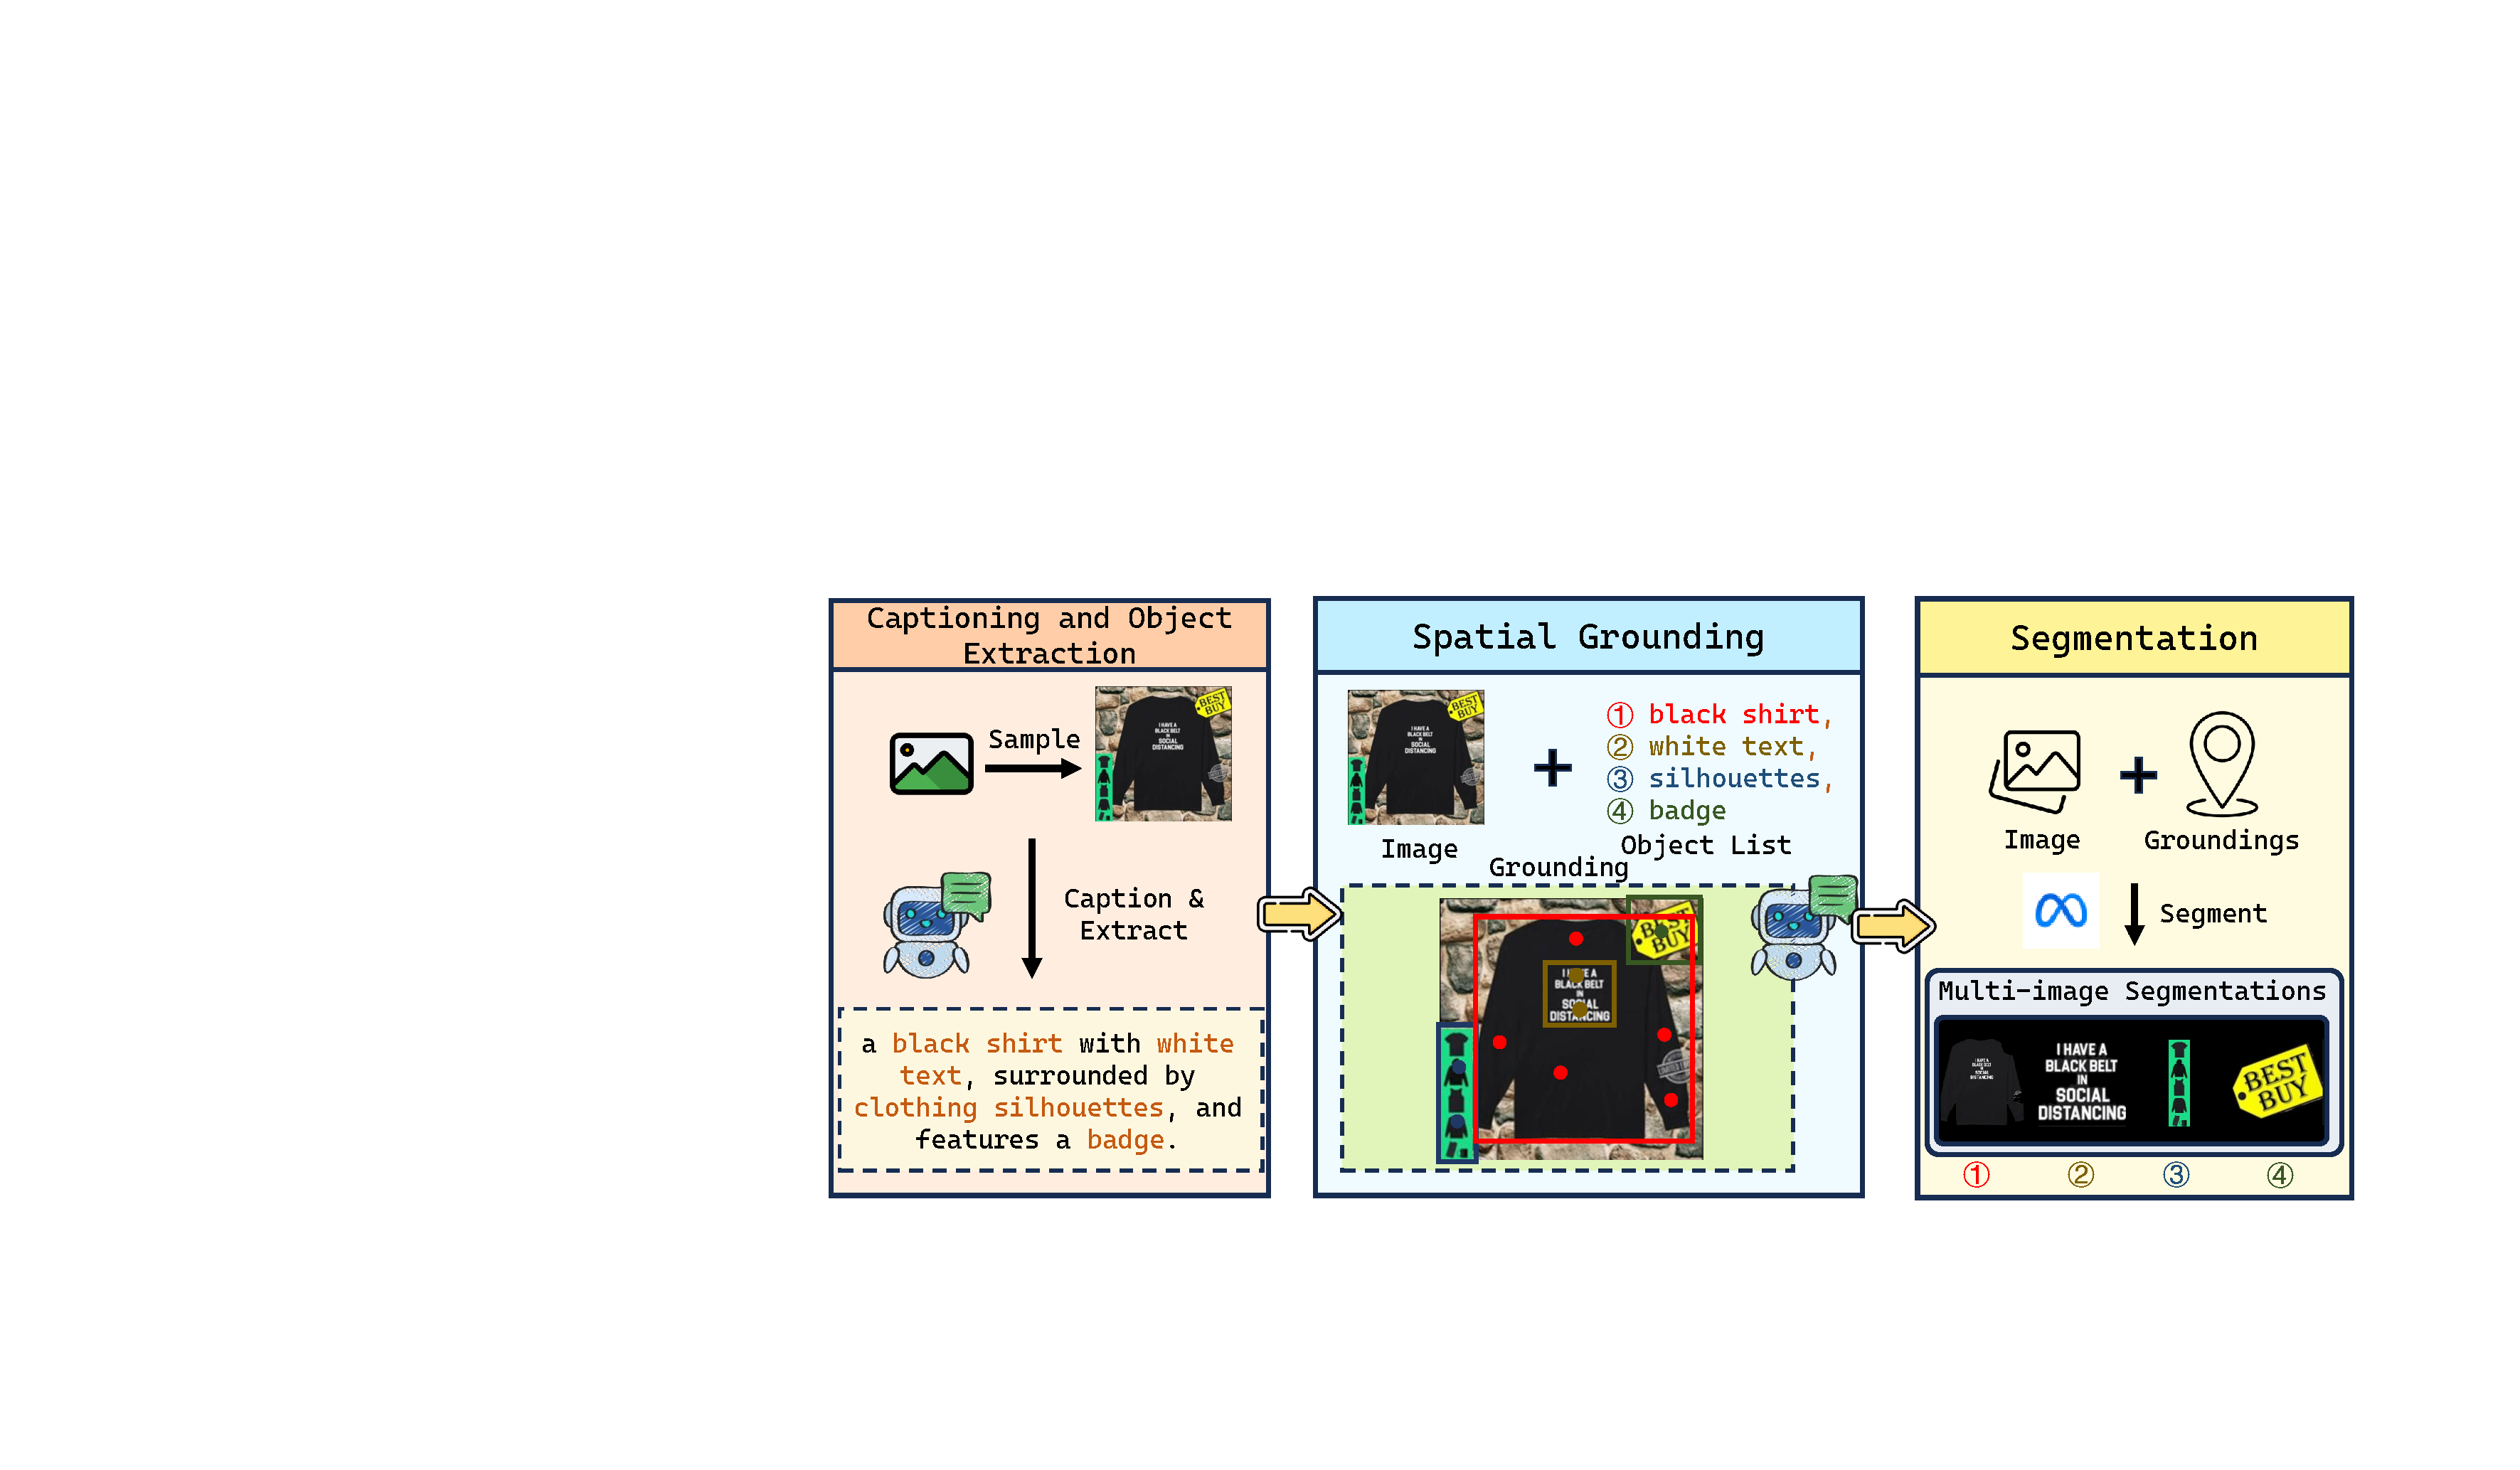
\includegraphics[width=1.0\textwidth]{figures/data_construct.pdf}
\caption{Illustration of the automatic data generation pipeline.}
\label{fig:construction}
\end{figure*}

\paragraph{Data Construction}
To support the large-scale training required for our two-stage paradigm, we developed an automated pipeline for generating high-quality multimodal training data, as shown in Figure~\ref{fig:construction}. This pipeline combines open-source image datasets with state-of-the-art vision-language models (VLMs) and segmentation models, enabling the construction of richly annotated image-text pairs with multiple segmented foreground objects without manual labeling:

\begin{itemize}[left=2pt]
\item \textbf{Captioning and Object Extraction:} A VLM is queried to generate a comprehensive caption describing prominent elements in the image, followed by extracting a list of concrete, distinct, and segmentable objects. This ensures that the generated data focus on tangible visual entities.
\item \textbf{Spatial Grounding:} For each extracted object, the VLM is queried again to identify its spatial location within the image, returning both a tight bounding box and several representative 2D keypoints. These spatial cues constrain the region of interest for subsequent segmentation, improving accuracy and reducing background noise.
\item \textbf{Segmentation:} A segmentation model is employed to extract object masks from the image, guided by the generated bounding boxes and keypoints. This step produces high-quality masks that are both semantically aligned with the object labels and spatially accurate.
\end{itemize}

By applying this automated process to a large corpus of open-source images, we construct a diverse multimodal dataset comprising captioned images annotated with multiple precisely segmented objects. This dataset forms a critical component of our training setup, particularly enabling the object segmentation and image recovery tasks in our training paradigm.


\section{Experiment Details}
\label{sec:Experiment_Details}

\subsection{Benchmark Details}
\label{sec:Benchmark_Details}

\paragraph{DreamBench++}
\label{app:DreamBench_Plus}

\textbf{Data Organization.}
DreamBench++~\citep{peng2025dreambenchpp} comprises 150 high-quality reference images, sourced from Unsplash, Rawpixel, and Google Images, encompassing a balanced mix of subjects. These are evenly divided into three broad categories: \textit{objects}, \textit{living subjects} (humans and animals), and \textit{styles} (illustrative, painterly, etc.), ensuring visual and conceptual diversity.

In total, DreamBench++ offers \textbf{1,350 prompts} ($150 \times 9$), representing a substantial scale-up over the original DreamBench (30 subjects $\times$ 25 prompts). Relative to DreamBench, the dataset is \textbf{5$\times$ larger in subjects} and \textbf{54$\times$ larger in prompts}, enabling broader evaluation of generative performance.

\textbf{Evaluation Metric.}
DreamBench++ adopts an automatic, GPT-4o-based evaluation protocol designed to closely mirror human judgment. Each generated image is assessed against both its reference image and its corresponding prompt, using two complementary axes:

\begin{itemize}[left=2pt, itemsep=0.5pt,topsep=0.5pt]
\item \textbf{Concept Preservation (CP):} Measures fidelity between the generated image and the reference. Key attributes include shape, color, texture, and facial details.
\item \textbf{Prompt Following (PF):} Evaluates how well the generation aligns with the prompt in terms of relevance, accuracy, completeness, and contextual appropriateness.
\end{itemize}

Each axis is scored on a \textbf{five-level ordinal scale} from 0 (Very Poor) to 4 (Excellent), avoiding the complexity and bias of pairwise comparisons.

\paragraph{DreamBench}
The original DreamBench~\citep{ruiz2023dreamboothfinetuningtexttoimage} dataset consists of 30 subjects, each paired with 25 prompts, totaling 750 prompt-image pairs. It serves as a foundational benchmark for evaluating personalized image generation models, focusing on the model's ability to maintain subject identity across diverse prompts.


\subsection{Baselines}
\label{sec:Baselines_Details}

We compare our method against various baselines, categorized as follows:

\begin{itemize}[left=2pt, itemsep=0.5pt,topsep=0.5pt]
\item \textbf{Textual Inversion}~\citep{gal2022imageworthwordpersonalizing} learns a new word embedding to represent a specific concept, enabling personalized image generation by incorporating the new token into prompts. It requires a few images of the subject and fine-tunes the embedding without altering the base model weights.
\item \textbf{DreamBooth}~\citep{ruiz2023dreamboothfinetuningtexttoimage}: DreamBooth fine-tunes a pre-trained text-to-image model to bind a unique identifier with the subject's visual concept, allowing for personalized generation. It requires several images of subject and modifies model weights to capture subject-specific details.

\item \textbf{BLIP-Diffusion}~\citep{li2023blipdiffusionpretrainedsubjectrepresentation}: This approach introduces a pre-trained multimodal encoder to provide subject representations for the diffusion generator, enabling controllable multimodal image generation. 

\item \textbf{KOSMOS-G}~\citep{Kosmos-G}: KOSMOS-G is a multimodal large language model designed for zero-shot image generation from interleaved vision-language inputs, including multiple images and text. It aligns the output space of a transformer-based causal language model with a diffusion-based image decoder using a lightweight AlignerNet and compositional instruction tuning. This architecture enables KOSMOS-G to perceive complex multimodal prompts and generate coherent, subject-driven images without modifying the base image decoder.

\item \textbf{Emu2}~\citep{emu2}: Emu2 is a 37-billion-parameter generative multimodal model trained on large-scale multimodal sequences with a unified autoregressive objective. It exhibits strong in-context learning abilities for various multimodal tasks, including visual prompting and object-grounded generation.

\item \textbf{IP-Adapter}~\citep{ye2023ip-adapter}: IP-Adapter is a lightweight adapter that enables image prompt capability for pre-trained text-to-image diffusion models. It integrates image features into the generation process without modifying the base model, supporting flexible and efficient image-to-image generation.

\item \textbf{DreamEngine}~\citep{dreamengine}: DreamEngine is a unified framework that integrates multimodal encoders with diffusion models through a two-stage training approach, enabling advanced text-image interleaved control and achieving state-of-the-art performance in generating images with complex, concept-merged inputs.

\item \textbf{Unified-IO 2}~\citep{lu2023unifiedio2}: Unified-IO 2 is an autoregressive multimodal model capable of understanding and generating images, text, audio, and actions. It tokenizes various modalities into a shared semantic space and processes them with a single encoder-decoder transformer. Trained from scratch on a large multimodal pre-training corpus and fine-tuned on an ensemble of 120 datasets, Unified-IO 2 achieves state-of-the-art performance on the GRIT benchmark and strong results across more than 35 benchmarks. 

\item \textbf{Lumina-mGPT}~\citep{2024lumina}: Lumina-mGPT is a multimodal autoregressive models designed for flexible photorealistic text-to-image generation. It employs a pretrained decoder-only transformer as a unified framework for modeling multimodal token sequences. Through multimodal Generative PreTraining (mGPT) and subsequent Flexible Progressive Supervised Finetuning (FP-SFT) and Omnipotent Supervised Finetuning (Omni-SFT), Lumina-mGPT demonstrates versatile multimodal capabilities, including visual generation tasks, controllable generation tasks and vision-language tasks. 

\end{itemize}



\section{Qualitative Study}
\label{sec:Qualitative_Study}

\subsection{Image Reconstruction}
\label{sec:Reconstruction}

\begin{figure*}[t]
\centering
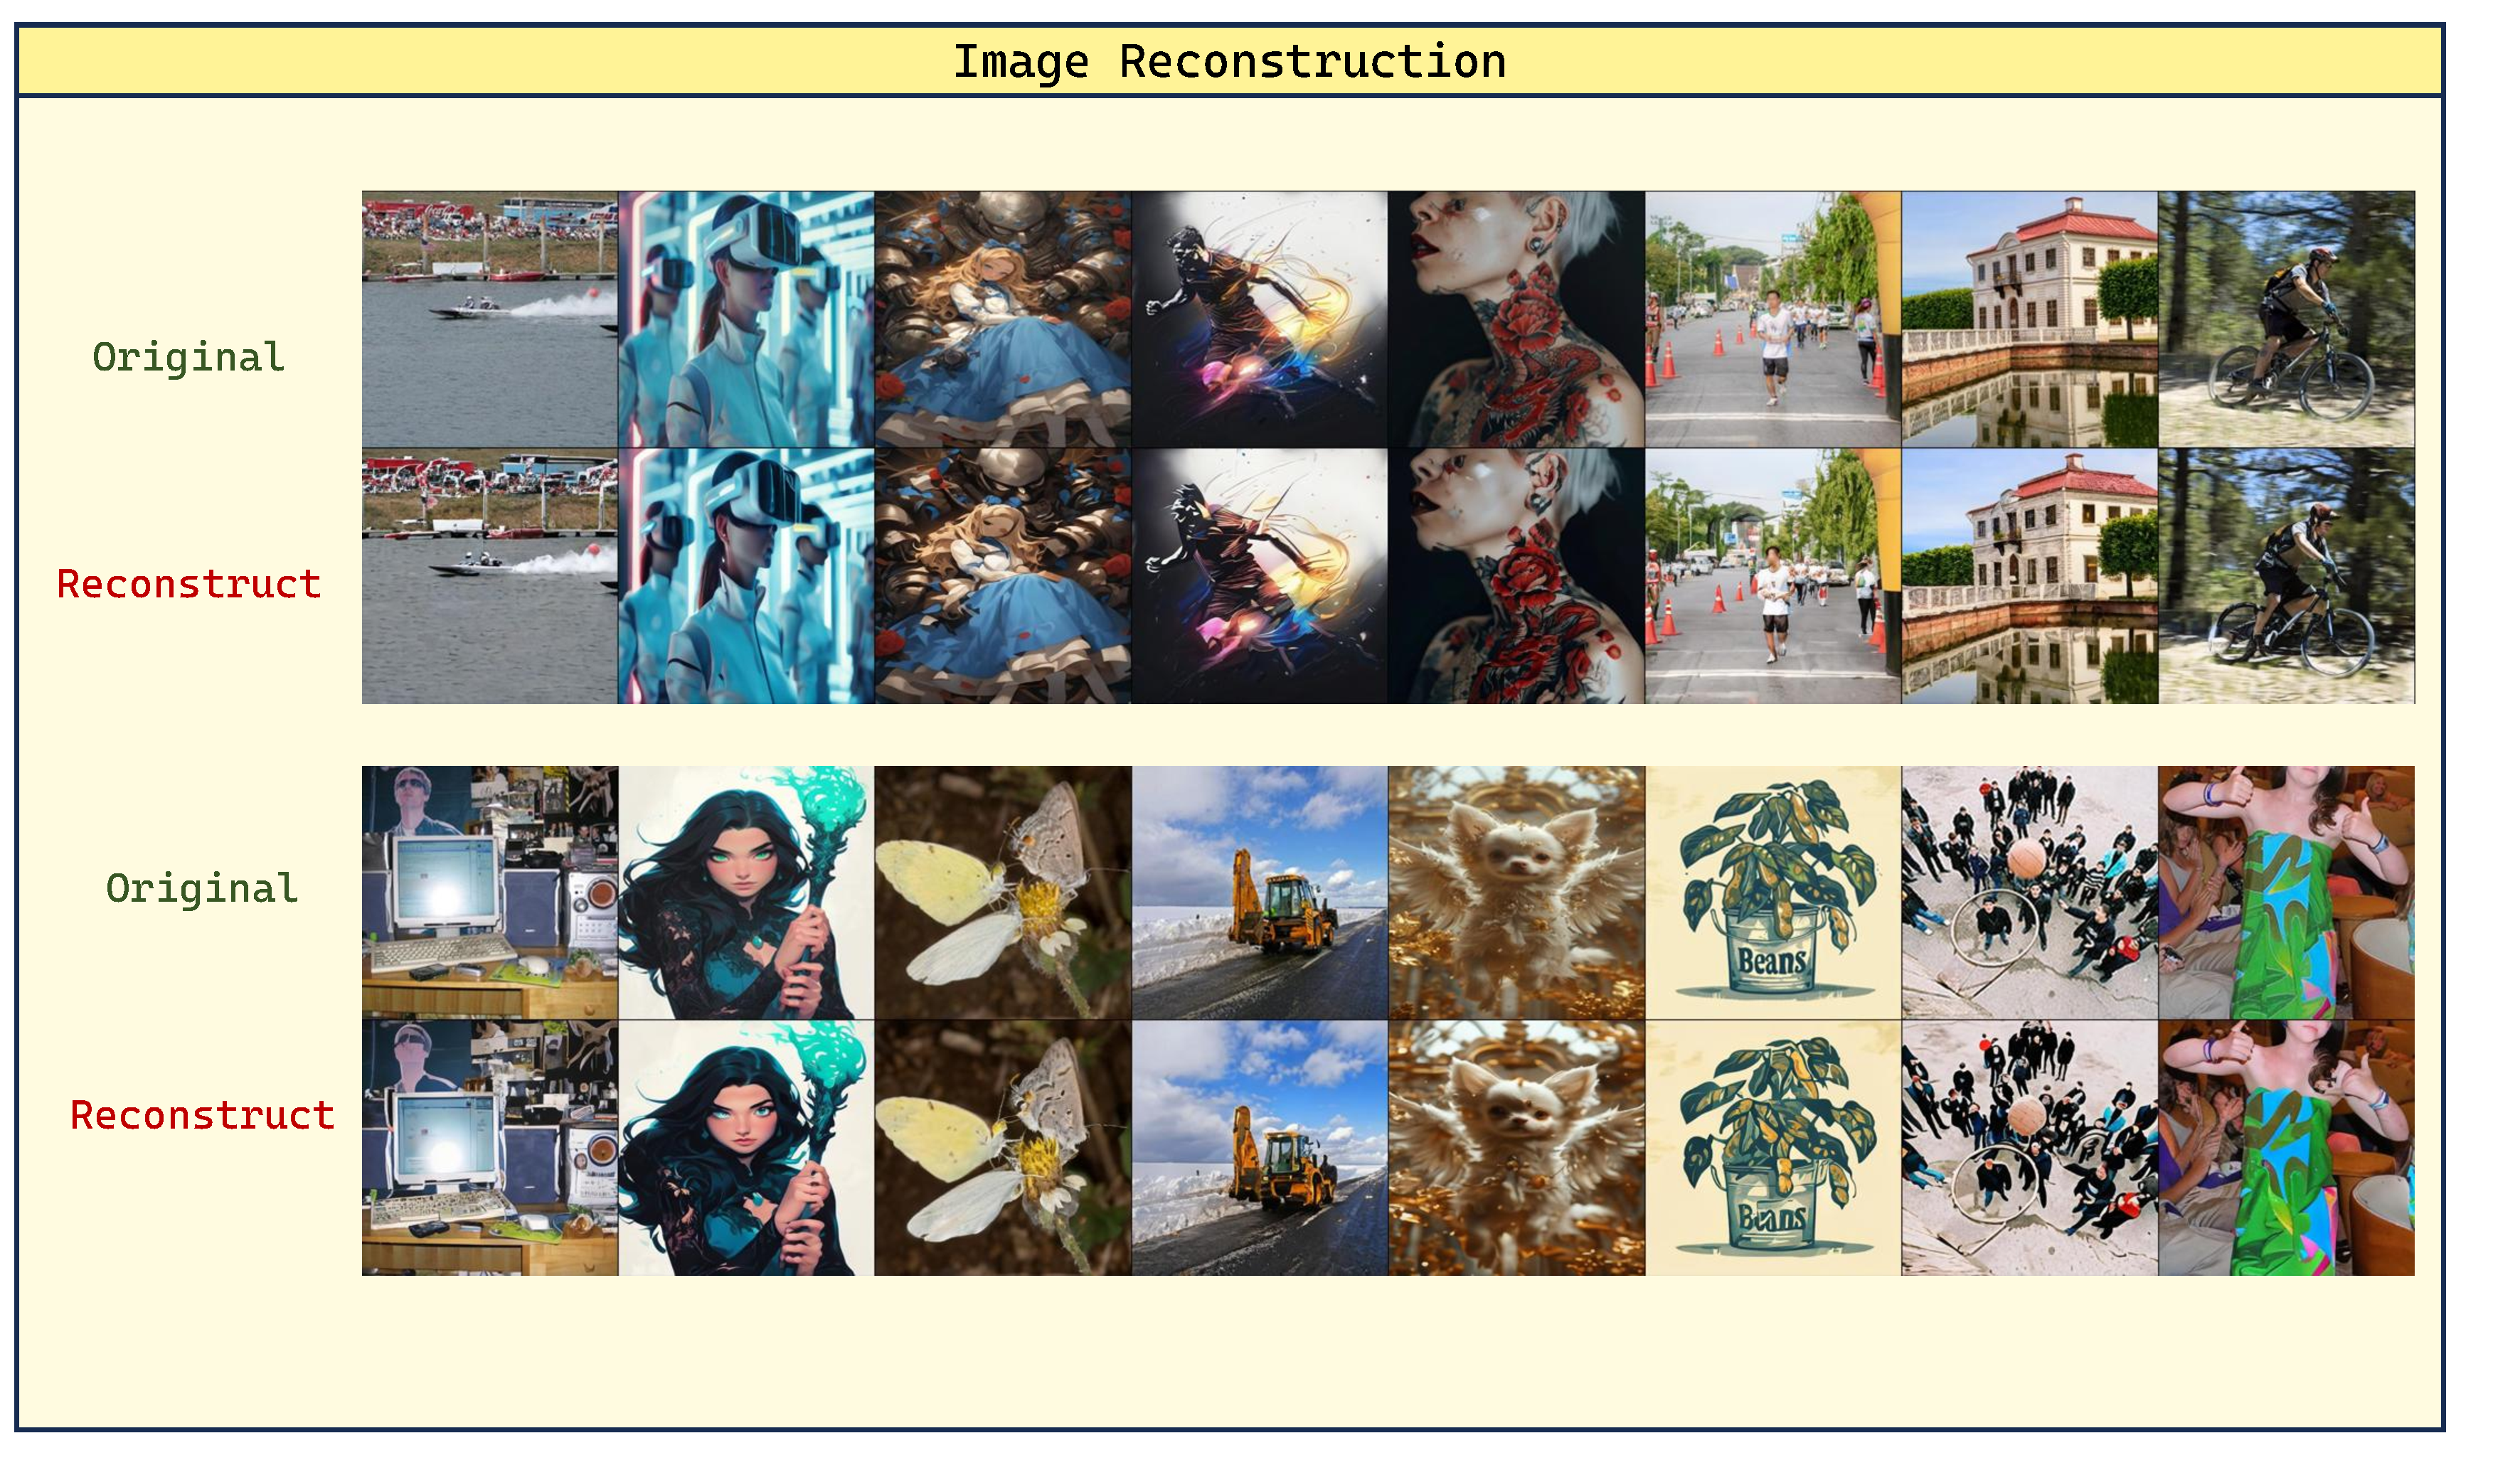
\includegraphics[width=0.85\textwidth]{figures/reconstrucion.pdf}
\caption{Qualitative comparison of image reconstruction results using \model.}
\label{fig:reconstruction}
\end{figure*}

\begin{figure*}[t]
\centering
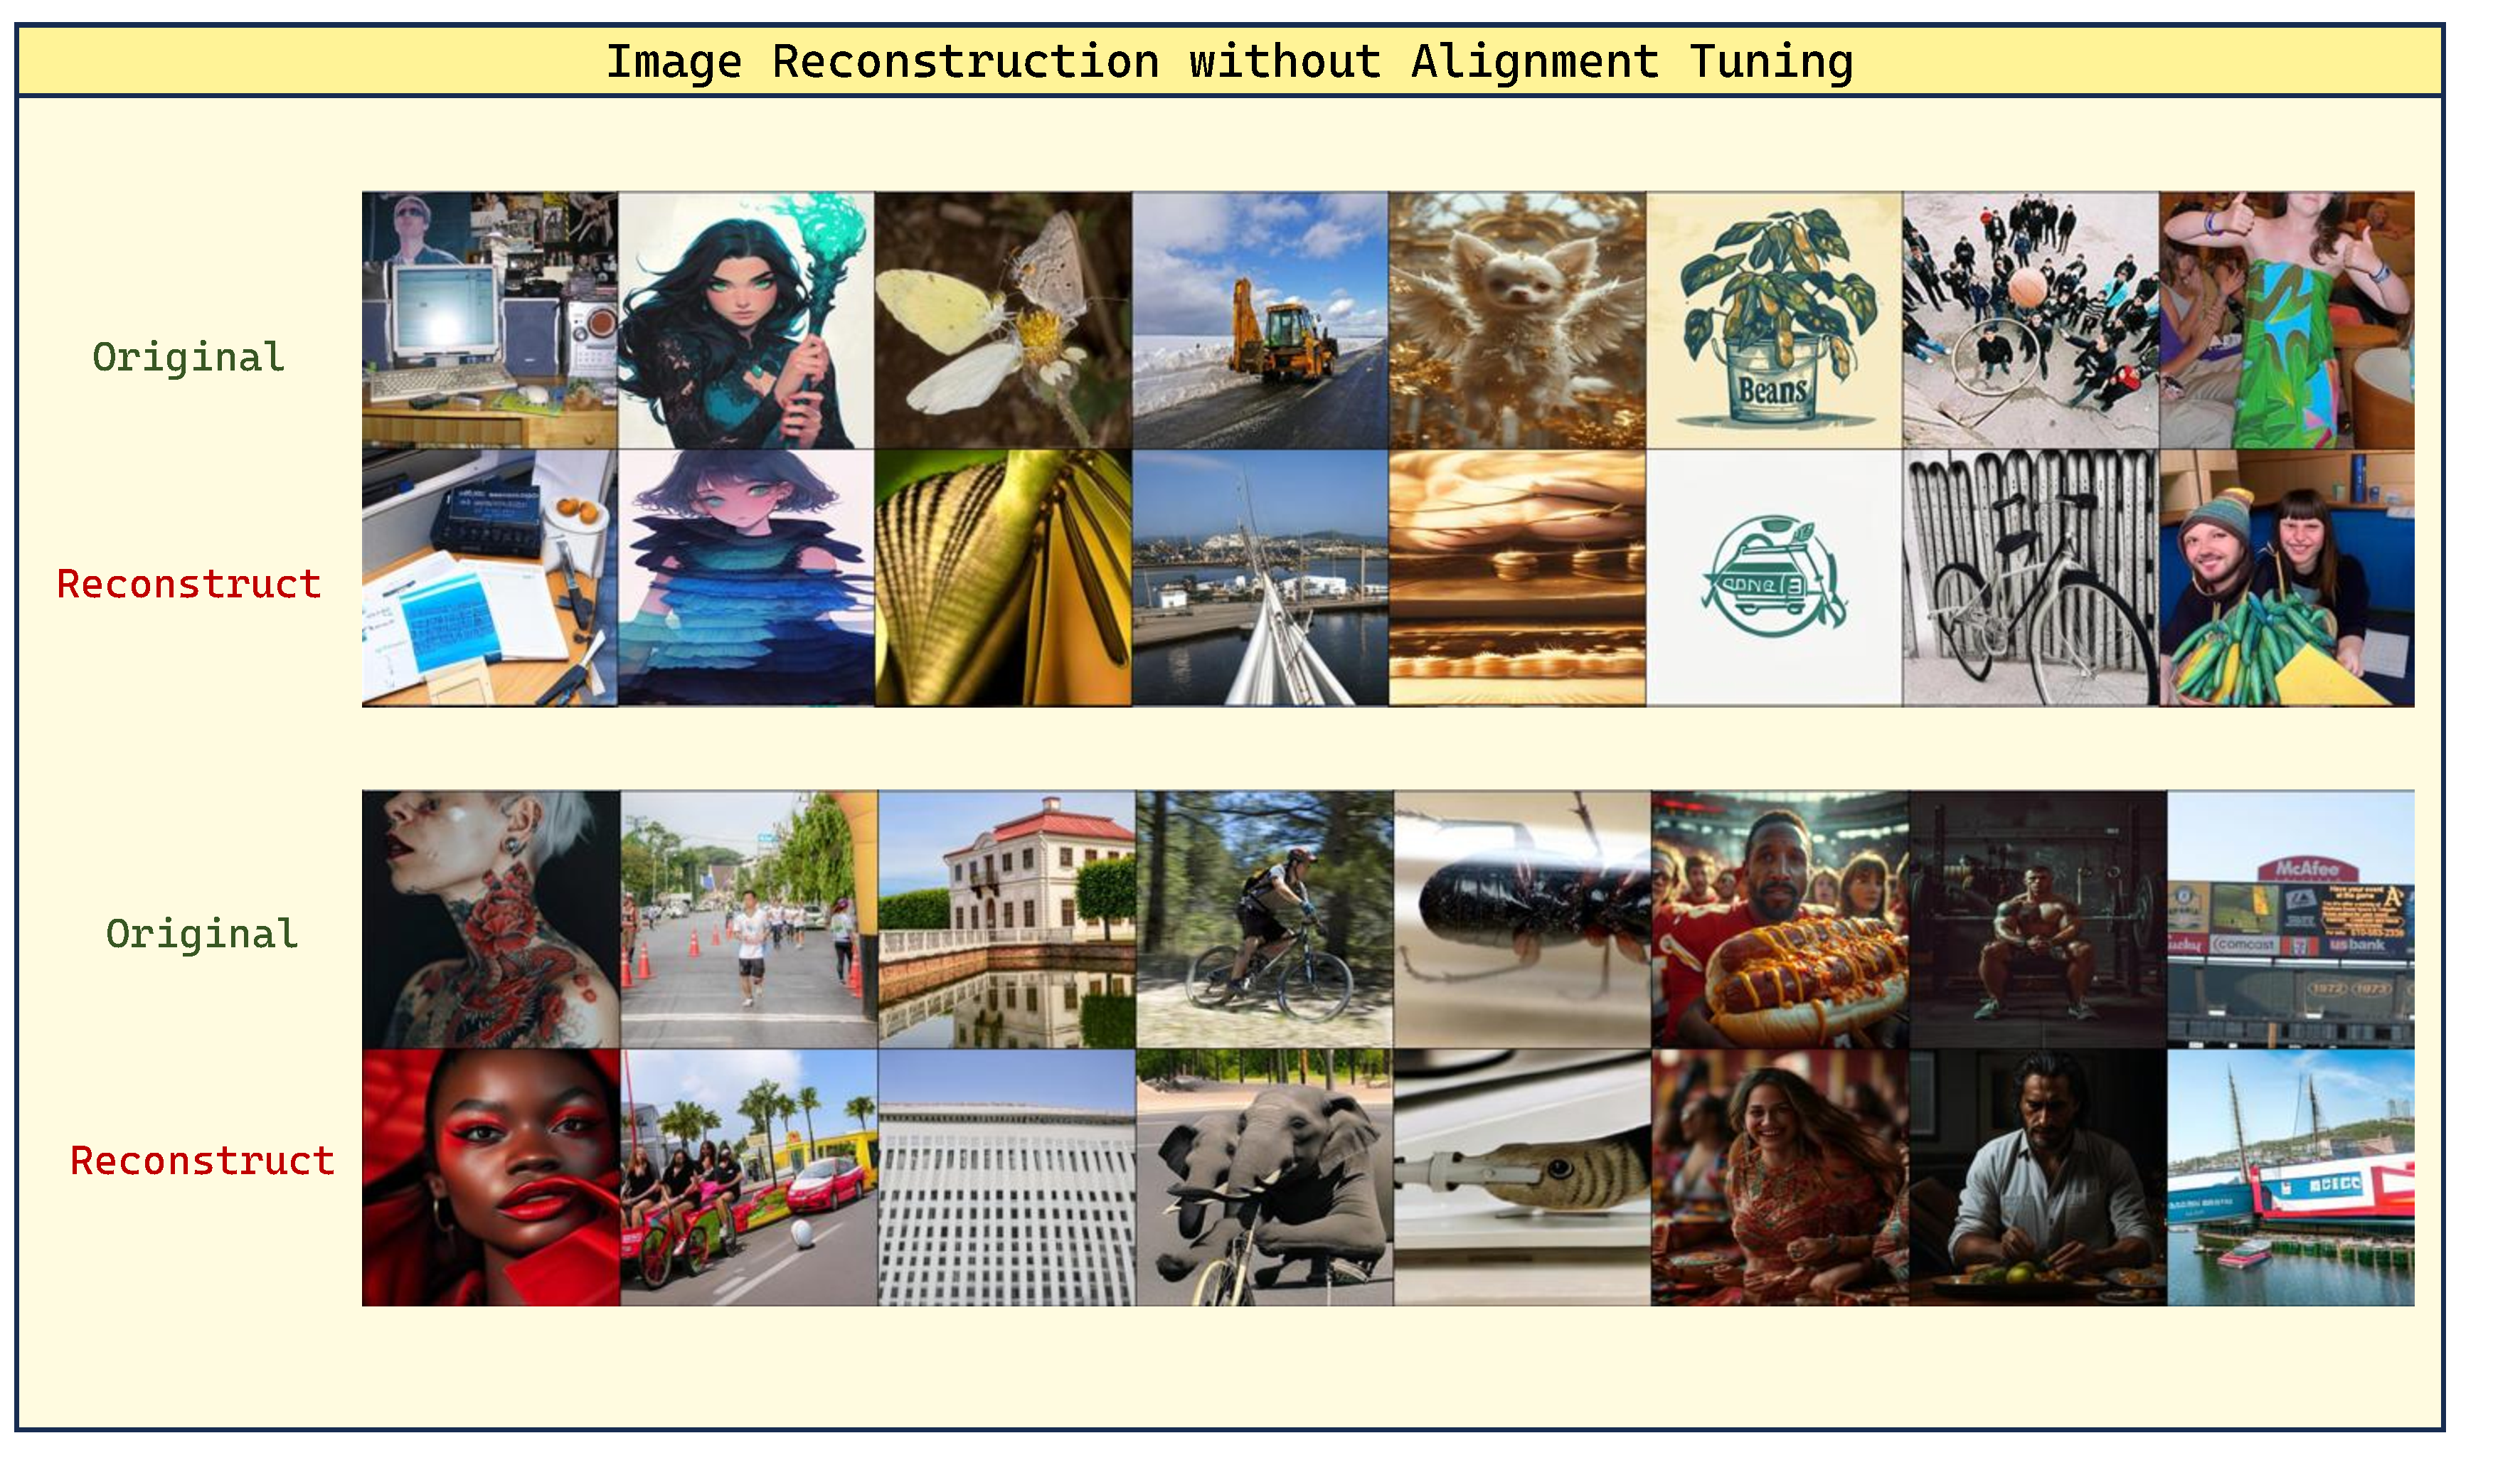
\includegraphics[width=0.85\textwidth]{figures/reconstrucion_wo_alignment.pdf}
\caption{Image reconstruction results of \model \textit{without} alignment tuning.}
\label{fig:reconstruction_wo_align}
\end{figure*}

As illustrated in Figures~\ref{fig:reconstruction} and \ref{fig:reconstruction_wo_align}, \model demonstrates strong image reconstruction capabilities following two-stage training. Notably, it is able to effectively reconstruct input images and preserve fine-grained visual details, even when input images are of low resolution (224×224) and outputs are generated at 512×512 resolution.

In contrast, when alignment tuning is omitted, although the model benefits from the pretrained multimodal encoder and the proposed architecture, it tends to treat the input image as a visual prompt akin to a caption. As shown in Figure~\ref{fig:reconstruction_wo_align}, this leads to outputs that resemble descriptive interpretations of the input rather than faithful reconstructions. Consequently, visual fidelity and spatial consistency degrade significantly without alignment tuning.

\subsection{Text-guided Image Segmentation}
\label{sec:Segmentation}


\begin{figure*}[t]
\centering
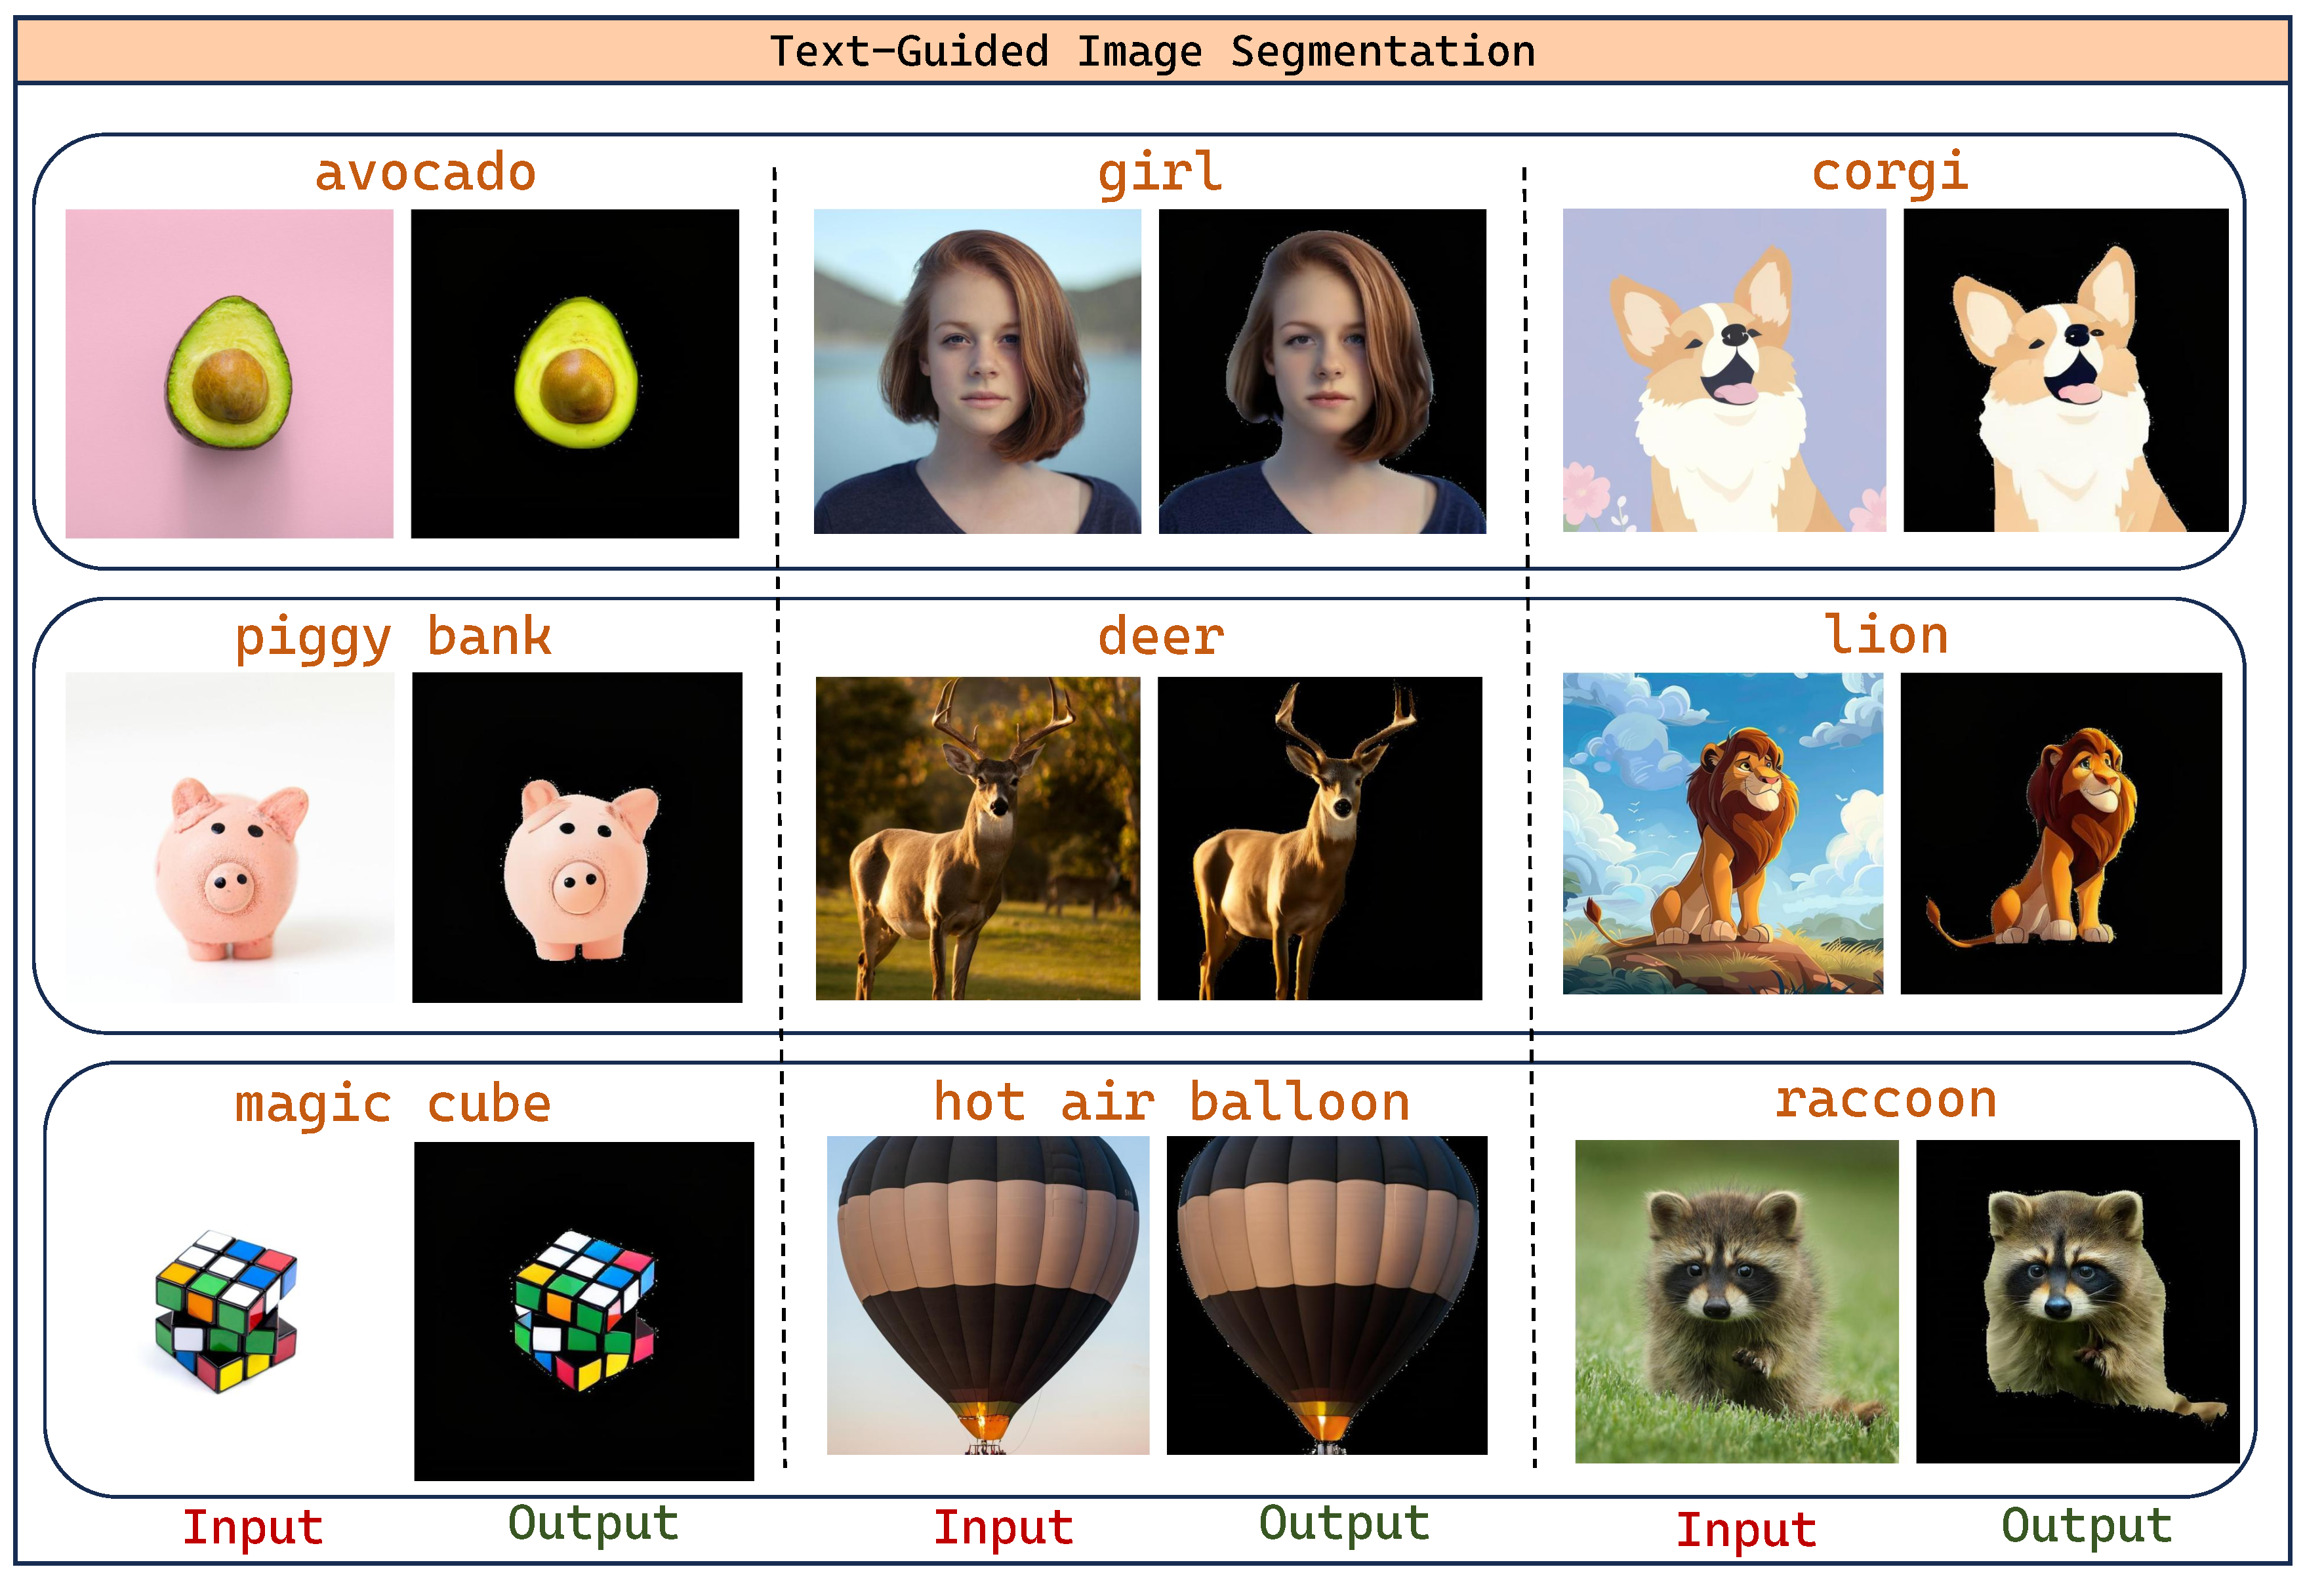
\includegraphics[width=1.0\textwidth]{figures/segmentation_example.pdf}
\caption{Qualitative results of text-guided image segmentation using \model.}
\label{fig:segmentation_example}
\end{figure*}

We evaluate \model on the DreamBench\texttt{++} benchmark to assess its performance in text-guided image segmentation. As demonstrated in Figure~\ref{fig:segmentation_example}, \model successfully identifies and segments visual concepts corresponding to the given textual prompts. These results highlight the model's ability to generalize across tasks and showcase its robust multimodal understanding and generation.

\subsection{Multi-Image Generation}
\label{sec:Multi-Image}

\begin{figure*}[t]
\centering
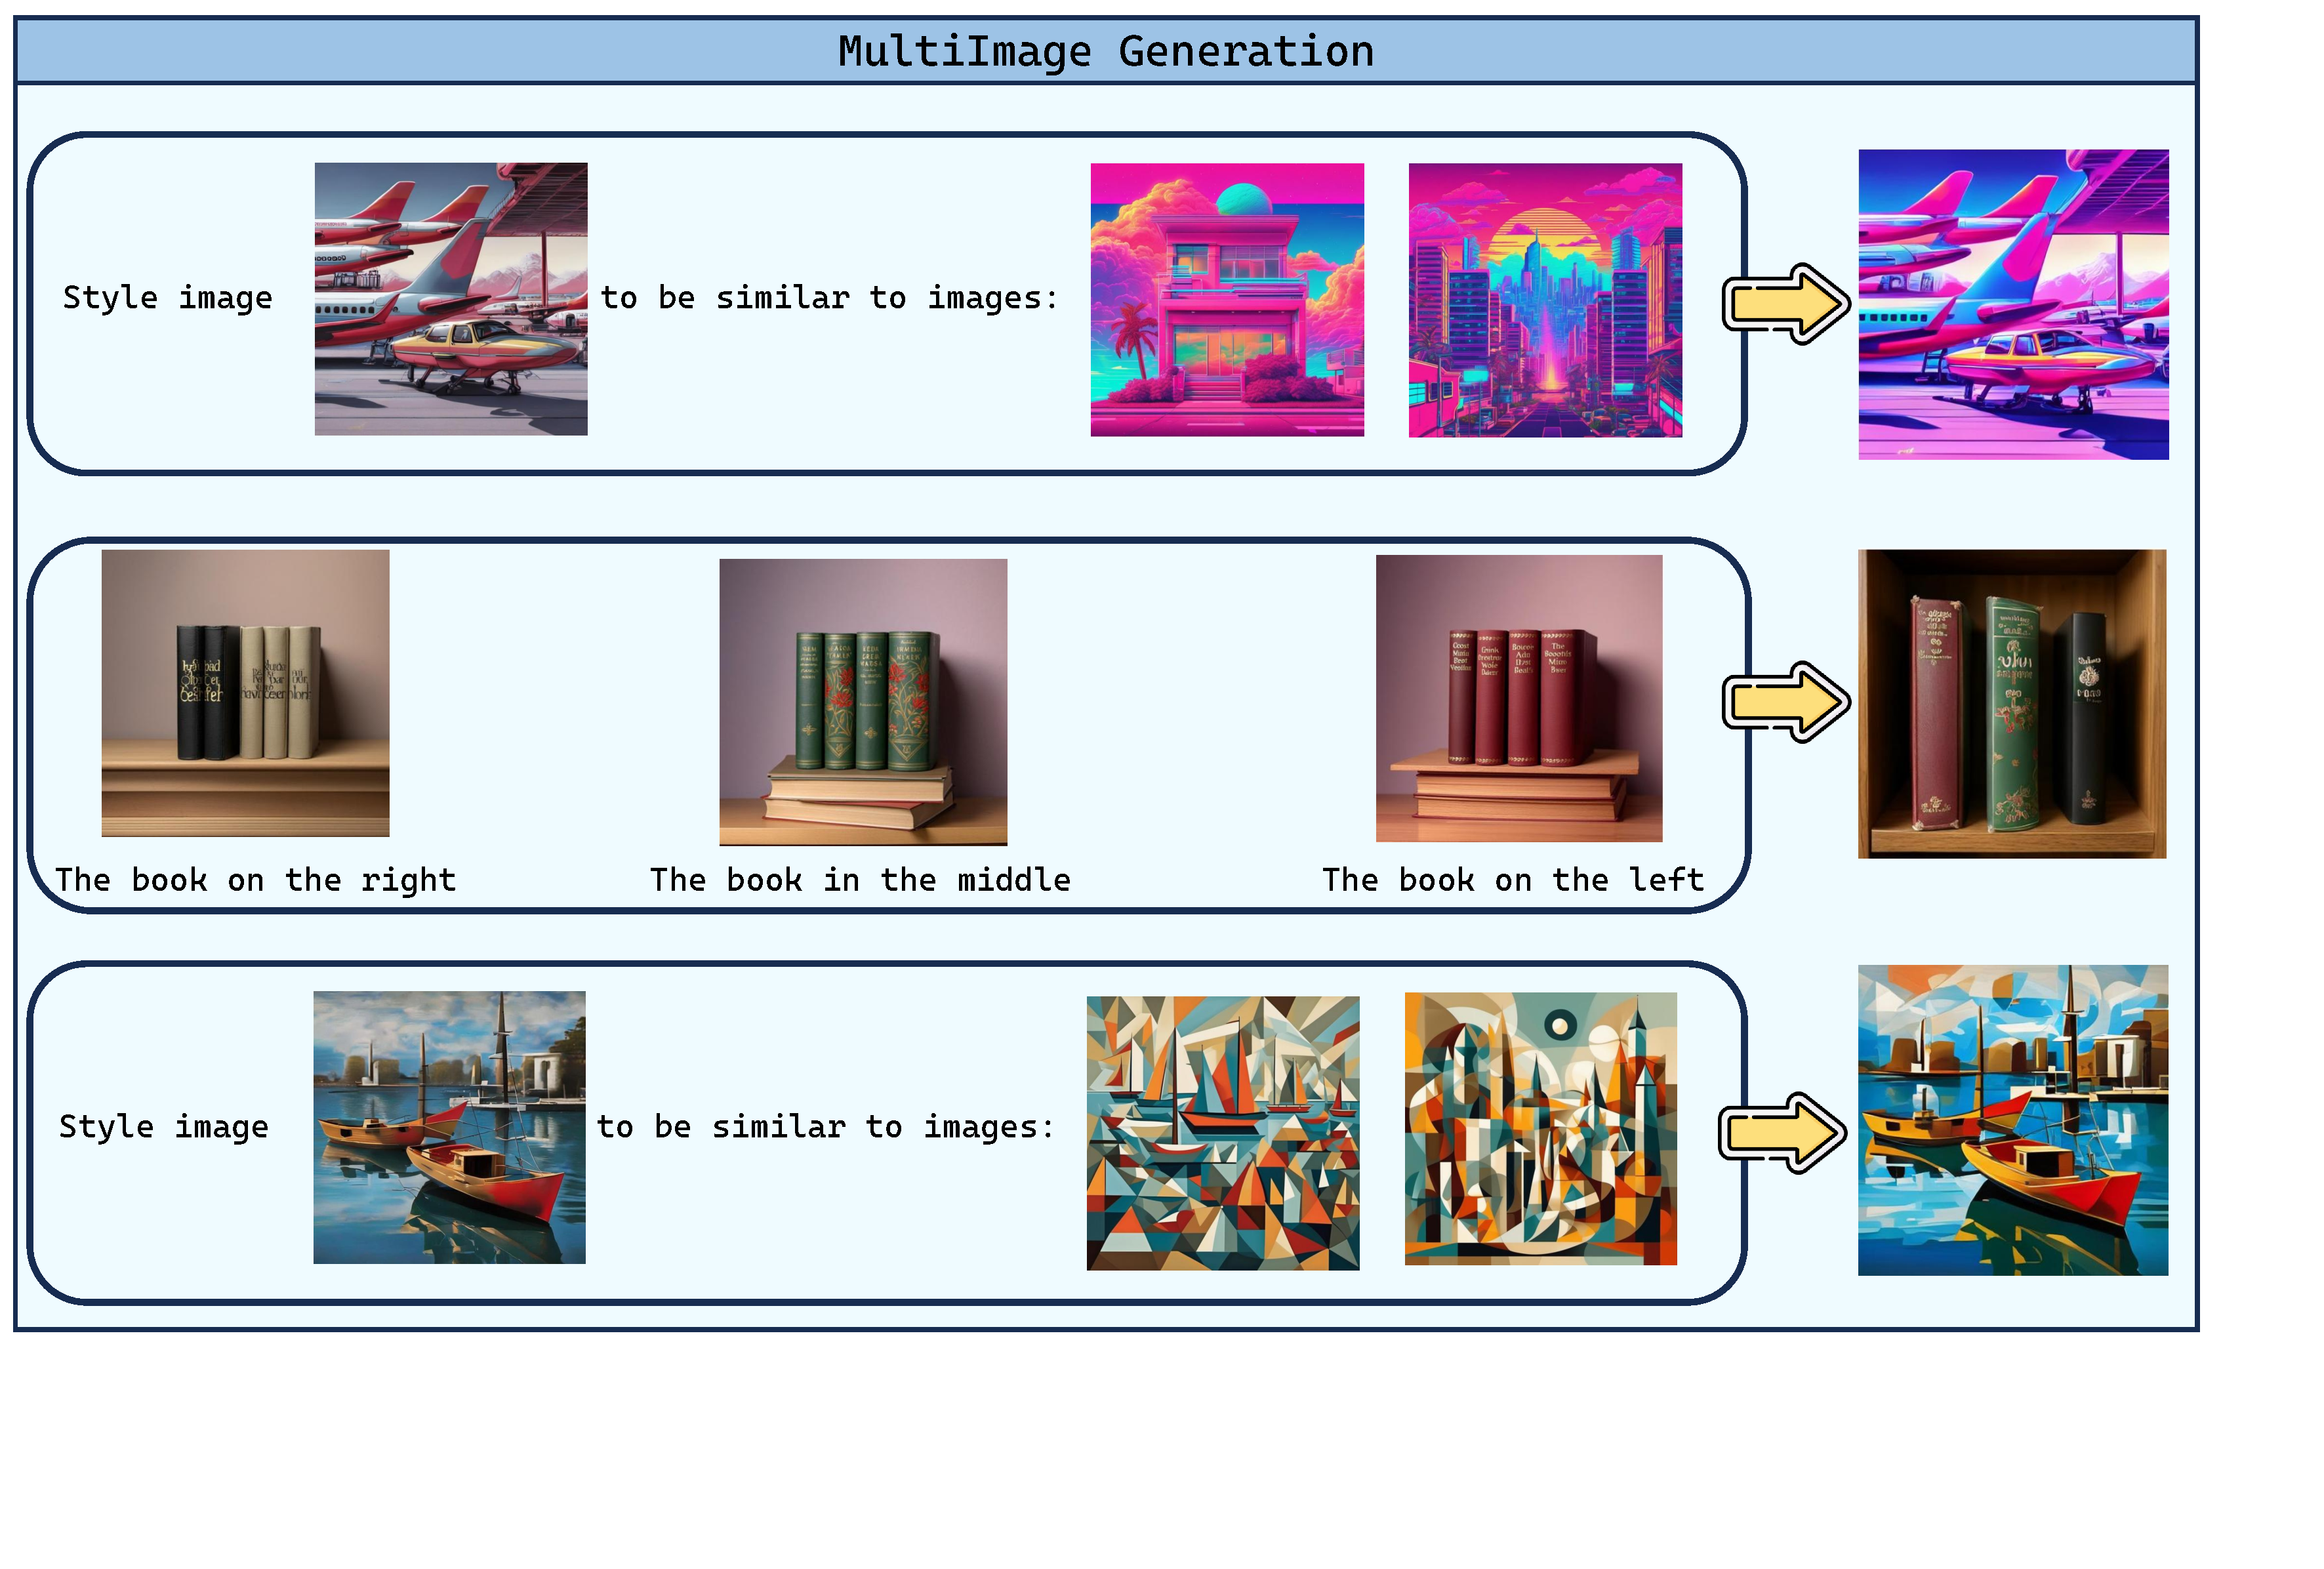
\includegraphics[width=0.85\textwidth]{figures/multi_img.pdf}
\caption{Qualitative results for multi-image generation.}
\label{fig:multi_image}
\end{figure*}

We evaluate \model on multi-image generation tasks using the X2I dataset~\citep{OmniGen}. As shown in Figure~\ref{fig:multi_image}, the model is capable of generating visually consistent outputs conditioned the multi-image inputs. The generated images reflect coherent semantics, style, and layout across the samples.

\subsection{Multimodal In-Context Image Generation}
\label{sec:mmicl}

\begin{figure*}[t]
\centering
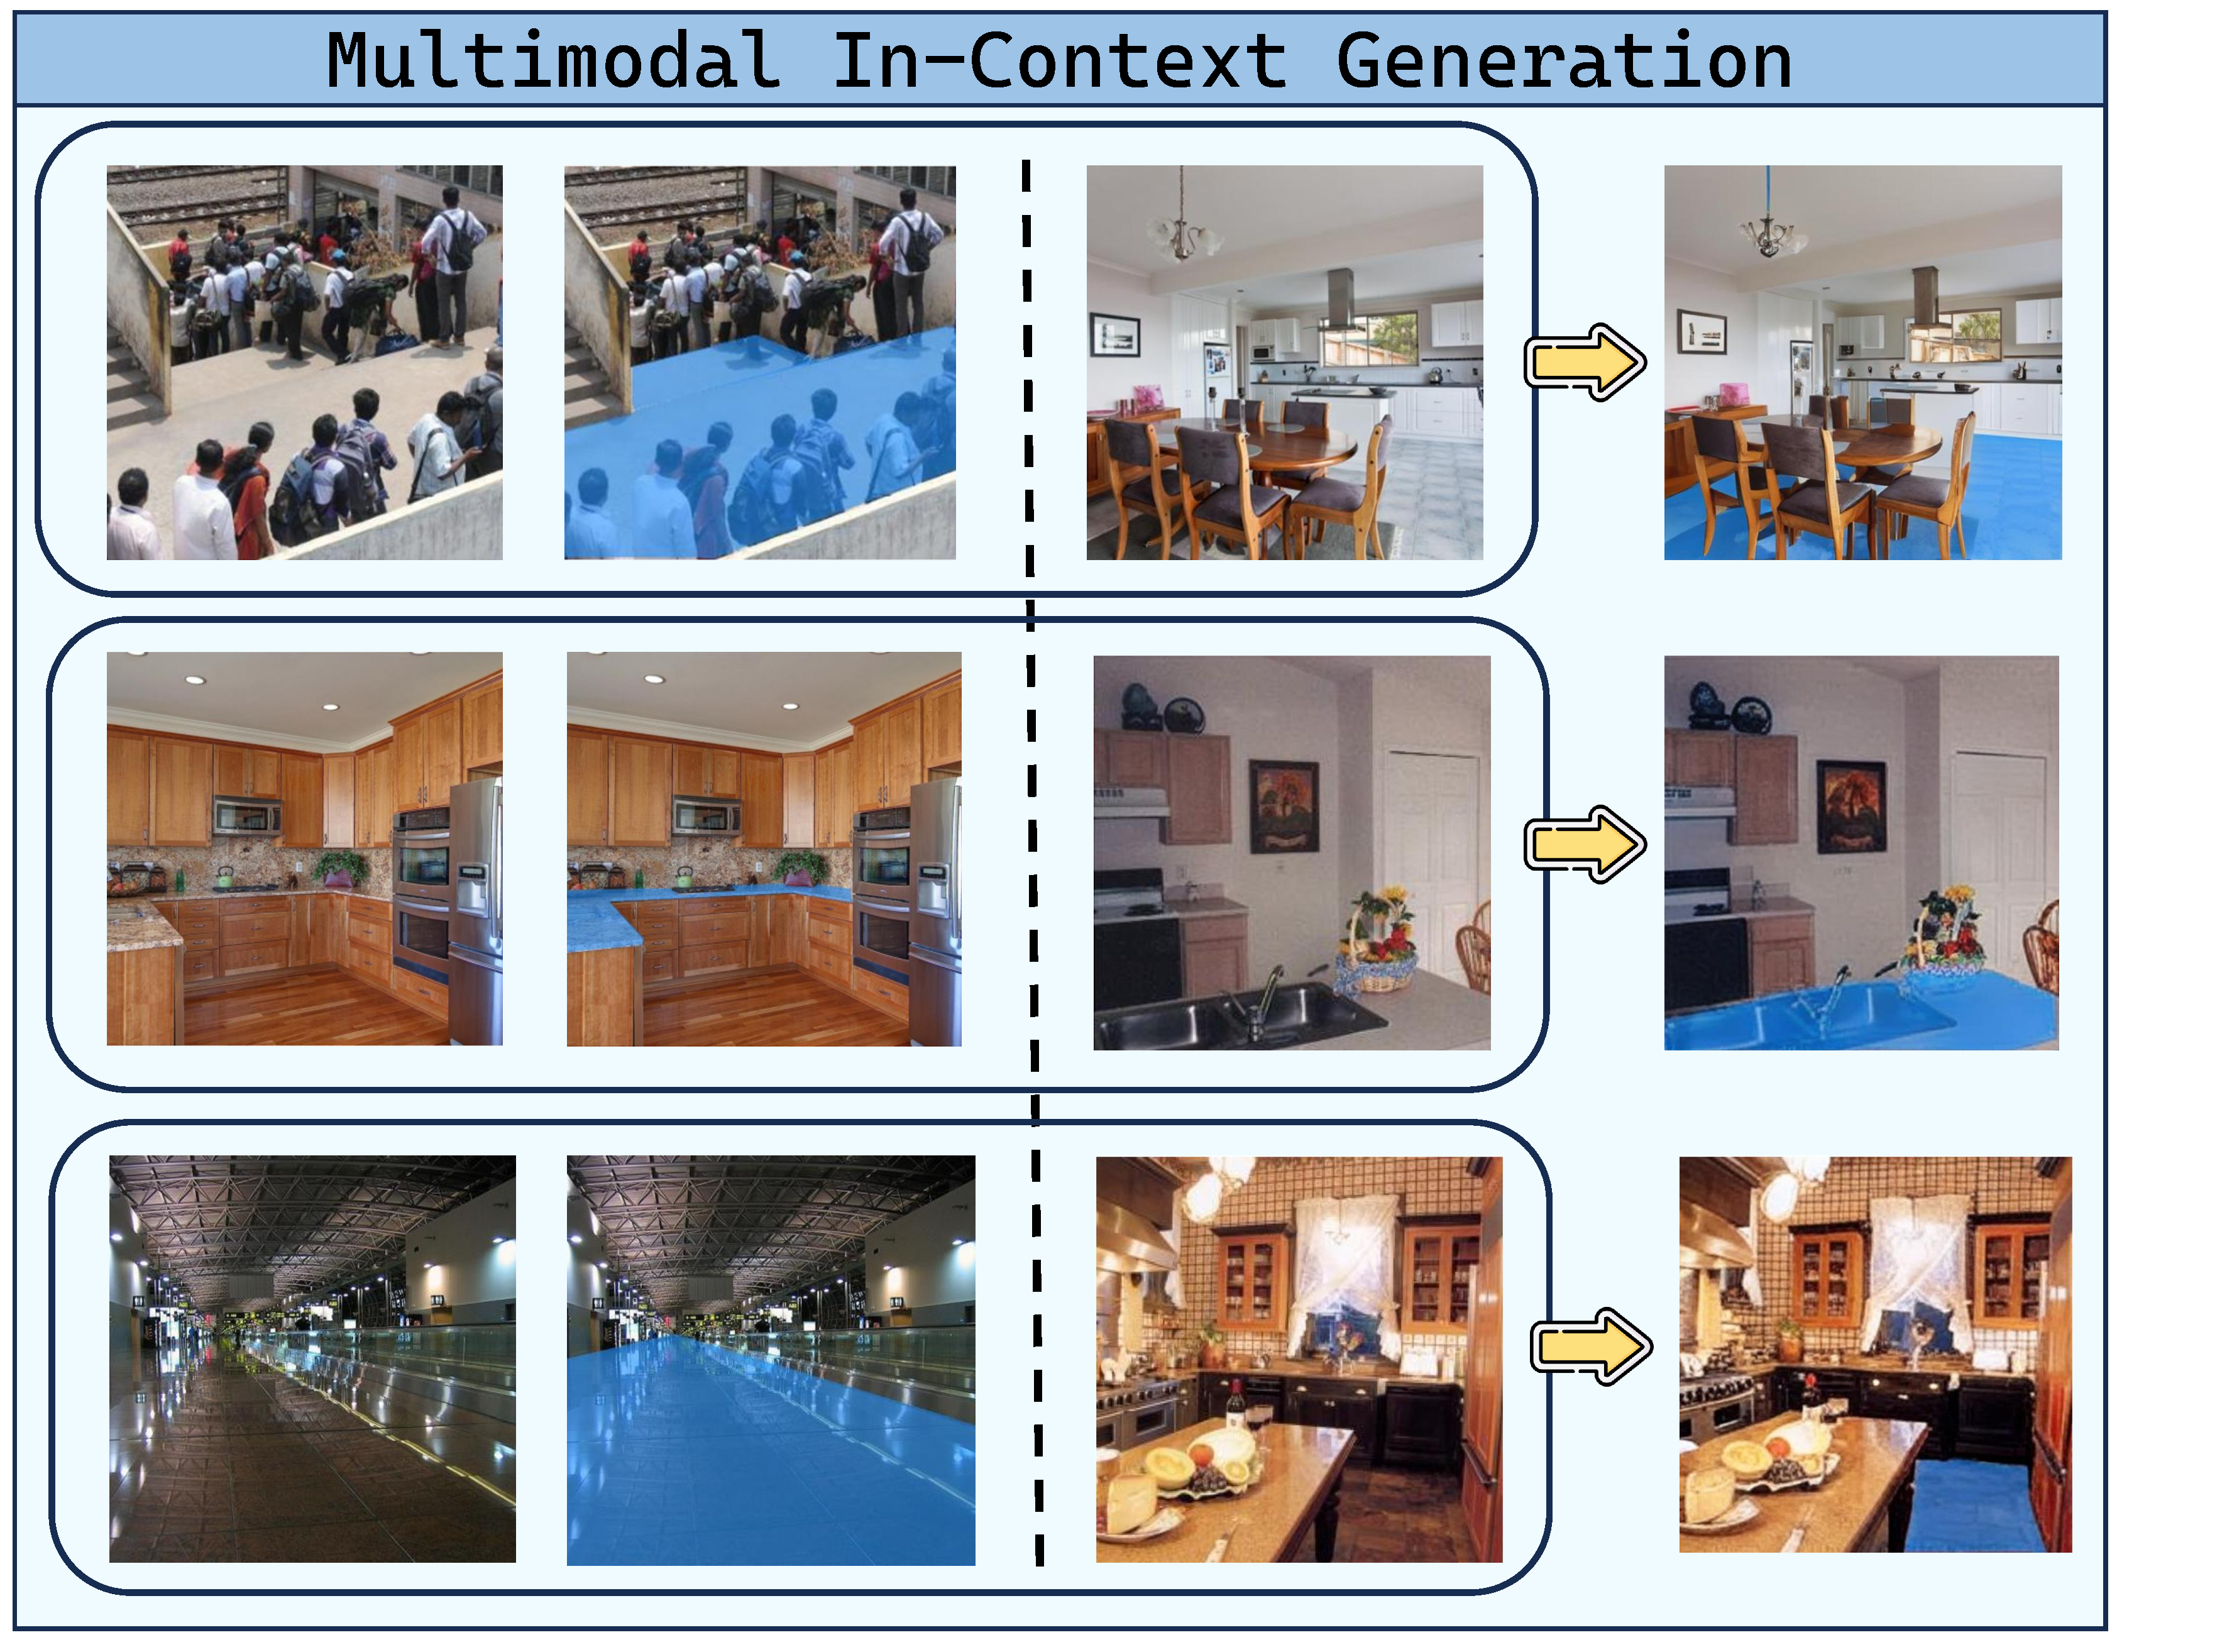
\includegraphics[width=0.75\textwidth]{figures/icl_exp.pdf}
\caption{Qualitative examples from multimodal in-context image generation. The model adapts to patterns in the visual context.}
\label{fig:icl_example}
\end{figure*}

To assess \model's few-shot generalization capabilities, we evaluate it on the multimodal in-context image generation task using the X2I-ICL dataset~\citep{OmniGen}. As illustrated in Figure~\ref{fig:icl_example}, \model learns to synthesize images that follow the stylistic patterns demonstrated in the in-context examples. This indicates its capability to infer complex visual trends and align generation with image context.

\section{Versatility Across Different Multimodal Tasks}
\label{app:applications}

To assess the broad applicability of our proposed framework, we evaluate \model across a diverse set of multimodal generation tasks, including text-guided image segmentation, subject-driven image generation, multi-image generation, and multimodal in-context learning. For each task, we apply supervised fine-tuning where necessary, ensuring robust generalization while maintaining architectural consistency.

\paragraph{Image Segmentation.}
We evaluate this task directly after Stage 1 training, without additional fine-tuning. The model demonstrates strong object localization and mask precision from prompt-aligned inputs, confirming the effectiveness of the proposed training pipeline and segmentation-aware data construction process.

\paragraph{Subject-driven Image Generation.}
This task is evaluated using the model at the end of Stage 2. No additional task-specific tuning is applied. The model successfully generates high-fidelity, identity-preserving images consistent with subject descriptors.

\paragraph{Multi-Image Generation.}
We fine-tune the Stage 2 model on a subset of X2I-subject-driven~\citep{OmniGen} dataset for two additional epochs using a reduced learning rate of $5 \times 10^{-5}$. All other optimization settings remain consistent with Stage 2. The dataset is split into disjoint training and test sets, and quantitative results are reported on the test split. The model learns to generate visually diverse yet semantically aligned images for the same input.

\paragraph{Multimodal In-Context Learning.}
We fine-tune the model for 10 epochs on the X2I-ICL dataset~\citep{OmniGen}, which features sequences of input-output pairs for in-context generalization. We use a learning rate of $5 \times 10^{-5}$ and ensure a strict train-test separation. The model adapts to context examples and generates new samples following the observed patterns, showing strong in-context learning performance without explicit prompting engineering.

\paragraph{Conclusion.}
The qualitative results presented in Section~\ref{sec:Qualitative_Study} confirm the versatility of \model across a wide range of tasks. Notably, the model adapts to each task without architectural modifications, requiring only lightweight fine-tuning.

\section{Limitations}
\label{app:limitation}

Our work presents a promising alternative to diffusion-based methods for multimodal-conditioned image generation. As such, our focus is on evaluating performance under comparable conditions—i.e., with similar model capacities and training paradigms.
However, the effectiveness of our approach is currently constrained by the limitations of available autoregressive (AR) backbone models. Due to the lack of high-performance AR generators, \model exhibits shortcomings in several aspects of image generation, including spatial reasoning, object counting, fine-grained human rendering, and stylization. These limitations reflect the current gap between current SOTA diffusion and autoregressive architectures in terms of generation fidelity and domain generalization.
Additionally, while our training data is sourced from publicly available datasets and our synthetic data pipeline includes NSFW safeguards, a comprehensive evaluation of safety, fairness, and potential misuse remains lacking. Future work should incorporate thorough assessments of model biases and unintended behaviors.
Finally, while our framework demonstrates strong versatility across diverse multimodal tasks, achieving competitive performance in specific domains may require more specialized training and the integration of more powerful multimodal encoders and generators. These initial findings nonetheless highlight the framework's potential as a unified and efficient foundation for conditional multimodal image generation.


% \bibliography{ref}
% \bibliographystyle{plainnat}

%%%%%%%%%%%%%%%%%%%%%%%%%%%%%%%%%%%%%%%%%%%%%%%%%%%%%%%%%%%%

\end{document}